\chapter{مقدمه}
	به «راهنمای استفاده از قالب \lr{\texttt{vruthesis}} جهت نگارش پایان‌نامه/رساله‌های دانشگاه ولی‌عصر (عج) رفسنجان» خوش‌آمدید. در صورتی که با \gls{typeset} با \lr{\LaTeX} و \lr{\XePersian} آشنایی دارید؛ پس از مطالعه‌ی فصل حاضر، می‌توانید به سرعت به \gls{typeset} رساله‌ی دکتری یا پایان‌نامه‌ی کارشناسی ارشد خود بپردازید. در کنار این راهنما، مجموعه‌ای از \glspl{file}ی نمونه نیز برای تسریع در فرایند آماده‌سازی رساله یا پایان‌نامه‌ی شما، قرار دارند.
	\section{شروعی سریع!}
	برای شروع، فرض می‌کنیم که شما قصد \gls{typeset} رساله یا پایان‌نامه‌ی خود را دارید و \glspl{file}ی نمونه را از \gls{site} علوم‌ریاضی، \gls{download} نموده‌اید. ابتدا، \gls{file} \lr{\texttt{thesis.tex}} را در ویرایشگر مورد علاقه‌ی خود، باز کنید. محتویات این \gls{file} برای \gls{typeset} یک پایان‌نامه‌ی کارشناسی ارشد، در شکل \ref{fig:ch1:thesis} نمایش داده‌ شده است. 
	
	\cite{Amintoosi09regional,Amintoosi09video,Amintoosi09precise,Amintoosi87afzayesh}
	
	\begin{figure}
		\centering\footnotesize
		\begin{mynewverbatim}
\documentclass[withpage,printonlyused,alg]{vruthesis}
% +rl|لطفا خطوط زیر را تغییر ندهید.$
\usepackage[extrafootnotefeatures]{xepersian}
\settextfont[Scale=1.3]{B Nazanin}
\defpersianfont\minutesfont[Scale=1.2]{B Nazanin}
\setlatintextfont{Times New Roman}
\setdigitfont[Scale=1]{Yas}
% لطفا هیچ تغییری در این فایل صورت ندهید.

\usepackage{subfig}
\usepackage{hyperref} % PDF links
\hypersetup{
	colorlinks = true, %Colours links instead of ugly boxes
	urlcolor = blue, %Colour for external hyperlinks
	linkcolor = blue, %Colour of internal links
	citecolor = red %Colour of citations
}
\usepackage[sanitizesort=false,sanitize={name=false},nomain,xindy,acronym,nonumberlist=true]{glossaries}
\usepackage[extrafootnotefeatures]{xepersian}
\usepackage[font={small},labelfont={normalsize,it}]{caption}
\settextfont[Scale=1.2]{B Nazanin}
\defpersianfont\minutesfont[Scale=1.2]{B Nazanin}
\setlatintextfont{Times New Roman}
\setdigitfont[Scale=1]{Yas}

\SepMark{-}
\newglossarystyle{fatoen}{%
	\renewenvironment{theglossary}{}{}
	\renewcommand*{\glsgroupskip}{\vskip \baselineskip}
	\renewcommand*{\glsgroupheading}[1]{\subsection*{\glsgetgrouptitle{##1}}}
	\renewcommand*{\glossentry}[2]{\noindent\glsentryname{##1}\dotfill\space \glsentrytext{##1}\par}
}
\newglossarystyle{entofa}{%
	\renewenvironment{theglossary}{}{}
	\renewcommand*{\glsgroupskip}{\vskip \baselineskip}
	\renewcommand*{\glsgroupheading}[1]{\begin{LTR} \subsection*{\lr{\glsgetgrouptitle{##1}}} \end{LTR}}
	\renewcommand*{\glossentry}[2]{\noindent\glsentrytext{##1}\dotfill\space \glsentryname{##1}\par}
}
\newglossarystyle{abbr}{%
	\renewenvironment{theglossary}{}{}
	\renewcommand*{\glsgroupskip}{\vskip \baselineskip}
	\renewcommand*{\glsgroupheading}[1]{}
	\renewcommand*{\glossentry}[2]{\noindent\glsentrytext{##1}\dotfill\space\Glsentrylong{##1}\par}
	\renewcommand*{\acronymname}{\hfill\rl{اختصارات و نمادها}\hfill}
}
\newglossary[glg]{english}{gls}{glo}{\rl{واژه‌نامه انگلیسی به فارسی}}
\newglossary[blg]{persian}{bls}{blo}{\rl{واژه‌نامه فارسی به انگلیسی}}
%\newglossary[glg]{english}{gls}{glo}{\hfill\rl{واژه‌نامه انگلیسی به فارسی}\hfill}
%\newglossary[blg]{persian}{bls}{blo}{\hfill\rl{واژه‌نامه فارسی به انگلیسی}\hfill}
\makeglossaries
\let\oldgls\gls
\let\oldglspl\glspl
\makeatletter
\renewrobustcmd*{\gls}{\@ifstar\@msgls\@mgls}
\newcommand*{\@mgls}[1] {\ifthenelse{\equal{\glsentrytype{#1}}{english}}{\oldgls{#1}\glsuseri{f-#1}}{\lr{\oldgls{#1}}}}
\newcommand*{\@msgls}[1]{\ifthenelse{\equal{\glsentrytype{#1}}{english}}{\glstext{#1}\glsuseri{f-#1}}{\lr{\glsentryname{#1}}}}
\renewrobustcmd*{\glspl}{\@ifstar\@msglspl\@mglspl}
\newcommand*{\@mglspl}[1] {\ifthenelse{\equal{\glsentrytype{#1}}{english}}{\oldglspl{#1}\glsuseri{f-#1}}{\oldglspl{#1}}}
\newcommand*{\@msglspl}[1]{\ifthenelse{\equal{\glsentrytype{#1}}{english}}{\glsplural{#1}\glsuseri{f-#1}}{\glsentryplural{#1}}}
\makeatother
\newcommand{\newword}[4]{
	\newglossaryentry{#1}     {type={english},name={\lr{#2}},plural={#4},text={#3},description={}}
	\newglossaryentry{f-#1} {type={persian},name={#3},text={\lr{#2}},description={}}
}
\defglsentryfmt[english]{\glsgenentryfmt\ifglsused{\glslabel}{}{\LTRfootnote{\glsentryname{\glslabel}}}}
\defglsentryfmt[acronym]{\glsentryname{\glslabel}\ifglsused{\glslabel}{}{\LTRfootnote{\glsentrydesc{\glslabel}}}}
\newcommand{\printabbreviation}{
	\cleardoublepage
	\pagestyle{empty}
	\phantomsection
	\baselineskip=.75cm
	\setglossarystyle{abbr}
	\begin{LTR}
		\Oldprintglossary[type=acronym]	
	\end{LTR}
	\clearpage
}
\newcommand{\printacronyms}{\printabbreviation}
\let\Oldprintglossary\printglossary
\renewcommand{\printglossary}{
	\let\appendix\relax
	\clearpage
	\phantomsection
	\addcontentsline{toc}{chapter}{واژه نامه انگلیسی به فارسی}
	\setglossarystyle{entofa}
	\Oldprintglossary[type=english]
	\clearpage
	\phantomsection
	\addcontentsline{toc}{chapter}{واژه نامه فارسی به انگلیسی}
	\setglossarystyle{fatoen}
	\Oldprintglossary[type=persian]
}
\newword{smallest}{\lr{Smallest Vertex Cover}}{\rl{کوچک‌ترین پوشش رأسی}}{\rl{}}
\newword{typeset}{\lr{Typesetting}}{\rl{حروف‌چینی}}{}
\newword{RandomVariable}{\lr{Random Variable}}{متغیر تصادفی}{متغیرهای تصادفی}
\newword{Action}{\lr{Action}}{کنش}{کنش‌ها} 
\newword{Optimization}{\lr{Optimization}}{بهینه‌سازی}{}
\newword{linked}{\lr{Linked List}}{\rl{لیست پیوندی}}{\rl{لیست‌های پیوندی}}
\newword{formatting}{\lr{Formatting}}{\rl{قالب‌بندی}}{}
\newword{file}{\lr{File}}{\rl{پرونده}}{\rl{پرونده‌ها}}
\newword{printer}{\lr{Printer}}{\rl{چاپگر}}{\rl{چاپگرها}}
\newword{site}{\lr{Web Site}}{\rl{وب‌گاه}}{\rl{وب‌گاه‌ها}}
\newword{flowchart}{\lr{Flow Chart}}{\rl{روندنما}}{\rl{روندنماها}}
\newword{inline}{\lr{Inline}}{\rl{داخلی}}{\rl{}}
\newword{lmatch}{\lr{Largest Matching}}{\rl{بزرگ‌ترین تطبیق}}{\rl{}}
\newword{bandwidth}{\lr{Bandwidth}}{\rl{پهنای‌باند}}{\rl{}}
\newword{download}{\lr{Download}}{\rl{دریافت}}{}

\newacronym{DFT}{\lr{DFT}}{\lr{Discrete Fourier Transform}}
\newacronym{QFT}{\lr{QFT}}{\lr{Quantum Fourier Transform}}
\newacronym[sort=alpha]{tensor}{\lr{$\otimes$}}{\rl{ضرب تانسوری}}
\newacronym{CDMA}{\lr{CDMA}}{\lr{Code Division Multiplexing Access}}
\newacronym{BAN}{\lr{BAN}}{\lr{Body Area Network}}
\newacronym{pdf}{\lr{PDF}}{\lr{Portable Document Format}}
\newacronym{gcd}{\rl{ب.م.م.}}{\rl{بزرگترین مقسوم‌علیه مشترک}}


\DefineVerbatimEnvironment{myverbatim}{Verbatim}{commandchars=+\[\]}
\DefineVerbatimEnvironment{mynewverbatim}{Verbatim}{commandchars=+|\$}

\makeatletter
	\newcommand*{\@thechapapp}{\@tartibi\c@chapter}
	\bidi@appto\appendix{\gdef\@thechapapp{\@harfi\c@chapter}}

	% ترتیبی کردن شماره فصل‌ها در فهرست مطالب در صورت استفاده از بسته hyperref
	\bidi@patchcmd{\Hy@org@chapter}{%
		\addcontentsline{toc}{chapter}%
		{\protect\numberline{\thechapter}#1}%
	}{%
		\addcontentsline{toc}{chapter}%
		{\protect\numberline{\@chapapp~\@thechapapp:}#1}%
	}{\typeout{We succeded in redefining \string\@chapter}}
	{\typeout{We failed in redefining \string\@chapter}}
	% اضافه کردن خط تیره بعد از شماره‌ فصل و بخش در متن
	%\renewcommand{\thesection}{\arabic{chapter}\@SepMark\arabic{section}\@SepMark}
	%\renewcommand{\thesubsection}{\arabic{chapter}\@SepMark\arabic{section}\@SepMark\arabic{subsection}\@SepMark}
	% اضافه کردن خط تیره بعد از شماره‌ها در فهرست مطالب و فهرست شکل ها و فهرست جدول ها
	\renewcommand{\cftsecaftersnum}{\@SepMark}%
	\renewcommand{\cftsubsecaftersnum}{\@SepMark}%
	\renewcommand{\cftfigaftersnum}{\@SepMark}%
	\renewcommand{\cfttabaftersnum}{\@SepMark}%
\makeatother

%%%%%%%%%%%%%%%%%%%%%%%%%%%%%%%
% زیاد کردن فاصله بین شماره‌ها و عنوان‌ها در فهرست مطالب
\setlength\cftchapnumwidth{4.5em}
\setlength\cftfignumwidth{3em}
\setlength\cfttabnumwidth{3em}
\setlength\cftsecnumwidth{2.5em}
\setlength\cftsubsecnumwidth{3.5em}
% زیاد کردن تورفتگی شماره‌ها و عنوان‌ها در فهرست مطالب
\setlength\cftsecindent{1.5em}
\setlength\cftsubsecindent{2.5em}

\renewcommand{\cfttoctitlefont}{\hspace*{\fill}\large\bfseries}
\renewcommand{\cftaftertoctitle}{\hspace*{\fill}}
\renewcommand{\cftlottitlefont}{\hspace*{\fill}\large\bfseries}
\renewcommand{\cftafterlottitle}{\hspace*{\fill}}
\renewcommand{\cftloftitlefont}{\hspace*{\fill}\large\bfseries}
\renewcommand{\cftafterloftitle}{\hspace*{\fill}}

%%%%%%%%%%%%%%%%%%%%%%%%%%%%%%%%%%%%%%%
% حروفی کردن شماره فصول و تغییر اندازه فونت فصول و بخش ها و زیر بخش ها
\titleformat{\chapter}[display]
  {\normalfont\large\bfseries}{\raggedright\chaptertitlename\ \tartibi{chapter}}{0pt}{\large\raggedright}
\titlespacing{\chapter}{2pc}{4cm}{1cm}[2pc]
\titleformat{\section}[block]{\bf{\normalfont\normalsize\bfseries}}{\thesection}{1em}{}
\titleformat{\subsection}[block]{\bf{\normalfont\small\bfseries}}{\thesubsection}{1em}{}
%%%%%%%%%%%%%%%%%%%%%%%%%%%%%%%%%%%%%%%
%حذف سطر اضافی بین دو مرجع متوالی در قسمت مراجع
\let\OLDthebibliography\thebibliography
\renewcommand\thebibliography[1]{
	\OLDthebibliography{#1}
	\setlength{\parskip}{0pt}
	\setlength{\itemsep}{0pt plus 0.3ex}
}
% ترتیبی کردن شماره فصل در سربرگ صفحات فرد
\renewcommand{\chaptermark}[1]{%
	\markboth{
		فصل \tartibi{chapter}~:~#1
	}{}
}
\makeatletter
	\bidi@patchcmd{\@harfi}{آ}{الف}
	{\typeout{Succeeded in changing `آ` into `الف`}}
	{\typeout{Failed in changing `آ` into `الف`}}
	\bidi@patchcmd{\@harfi}{ه}{هـ}
	{\typeout{Succeeded in changing `ه` into `هـ`}}
	{\typeout{Failed in changing `ه` into `هـ`}}
\makeatother

\let\oldAppendix\appendix
\renewcommand{\appendix}{
	\titleformat{\chapter}[display]
	{\normalfont\large\bfseries\flushleft}{\chaptertitlename\ \harfi{chapter}}{0pt}{\large}
	\oldAppendix
	\ifnofigures\else 
		\renewcommand{\thefigure}{\harfi{chapter}-\arabic{figure}} 
	\fi 
	\ifnotables\else 
		\renewcommand{\thetable}{\harfi{chapter}-\arabic{table}} 
	\fi
	\if@alg
		\renewcommand{\thealgorithm}{\harfi{chapter}-\arabic{algorithm}} 
	\fi
}

\setlength{\parskip}{0cm}

\renewcommand\citedash{\lr{--}}


% +rl|برای تعیین قالب ارجاع‌دهی؛ خط زیر را طبق راهنما، تغییر دهید.$
\bibliographystyle{ieeetr-fa-vru}
\begin{document}
% % % % % % % % % % % % % % % % % % % % %
	% % % % % % % % % % %
% نام دانشکده به همراه عنوان «دانشکده»
\faculty{دانشکده علوم‌ریاضی}
\facultyen{Mathematical Sciences}
% نام گروه آموزشی
\department{علوم کامپیوتر}
\departmenten{Computer Science}
% عنوان رشته‌ی تحصیلی
\subject{علوم کامپیوتر}
\subjecten{Computer Science}
% عنوان گرایش
\field{سیستم‌های هوشمند}
\fielden{Intelligent Systems}
% عنوان پایان‌نامه
\title{راهنمای استفاده از قالب \lr{\texttt{vruthesis}} جهت نگارش پایان‌نامه/رساله‌های دانشگاه ولی‌عصر (عج) رفسنجان}
\titleen{A Guide on how to use the \texttt{vruthesis} class to write Theses/Dissertations for Vali-e-Asr University of Rafsanjan}
\runtitle{عنوان کوتاه شده‌ی پایان‌نامه ...}
% نام و نام‌خانوادگی استاد راهنمای اول با پیشوند «دکتر»
\firstsupervisor{دکتر علی ...}
\firstsupervisoren{Dr. Ali ...}
% مرتبه‌ی علمی استاد راهنمای اول
\firstsupervisorrank{استادیار}
\firstsupervisorranken{Assistant Professor}
% اطلاعات استاد راهنمای دوم، در صورت وجود
\secondsupervisor{دکتر رضا ...}
\secondsupervisoren{Dr. Reza ...}
\secondsupervisorrank{استادیار}
\secondsupervisorranken{Assistant Professor}
% اطلاعات مشاور اول
\firstadvisor{دکتر محمد ...}
\firstadvisoren{Dr. Mohammad ...}
\firstadvisorrank{استادیار}
\firstadvisorranken{Assistant Professor}
% اطلاعات مشاور اول در صورت وجود
%\secondadvisor{دکتر حسین ...}
%\secondadvisoren{Dr. Hosein ...}
%\secondadvisorrank{استادیار}
%\secondadvisorranken{Assistant Professor}
% نام دانشجو
\name{علی}
\nameen{Ali}
% نام خانوادگی دانشجو
\surname{شکیبا}
\surnameen{Shakiba}
% ماه و سال دفاع - پس از ماه، عبارت «ماه» ذکر شود.
\thesisdate{آذر ماه ۱۳۹۶}
\thesisdateen{December 2017}
% تعداد واحد پایان‌نامه
\credit{۶}
\crediten{6}
% تاریخ دفاع
\defensedate{۱۳۹۶/۰۹/۳۰}
\defensedateen{December 21${}^{\text{st}}$, 2017}
% نمره‌ی دفاع
\grade{19.75}
\gradeen{19.75}
\letgrade{نوزده و هفتاد و پنج صدم}
\letgradeen{Ninteen and three quarters}
% درجه‌ی دفاع
\degree{عالی}
\degreeen{Excellent}
% اطلاعات داور داخلی اول
\firstinternalreferee{دکتر حسن ...}
\firstinternalrefereeen{Dr. Hasan ...}
\firstinternalrefereerank{استادیار}
\firstinternalrefereeranken{Assistant Professor}
% اطلاعات داور داخلی دوم
\secondinternalreferee{دکتر سجّاد ...}
\secondinternalrefereeen{Dr. Sajjad ...}
\secondinternalrefereerank{استادیار}
\secondinternalrefereeranken{Assistant Professor}
% اطلاعات داور خارجی اول
\firstexternalreferee{دکتر صادق ...}
\firstexternalrefereeen{Dr. Sadegh ...}
\firstexternalrefereerank{استادیار}
\firstexternalrefereeranken{Assistant Professor}
% اطلاعات داور خارجی دوم
\secondexternalreferee{دکتر باقر ...}
\secondexternalrefereeen{Dr. Bagher ...}
\secondexternalrefereerank{استادیار}
\secondexternalrefereeranken{Assistant Professor}
% اطلاعات ناظر تحصیلات تکمیلی
\viewer{دکتر کاظم ...}
\vieweren{Dr. Kazem ...}
\viewerrank{استادیار}
\viewerranken{Assistant Professor}
% متن تقدیم‌به
\totext{متن تقدیم به را در اینجا درج کنید}
% متن سپاسگزاری
\ack{متن سپاسگزاری را در اینجا درج کنید}
% متن چکیده فارسی
\abstractfa{چکیده‌ی خود را در اینجا قرار دهید}
% متن چکیده انگلیسی
\abstracten{Put your English abstract here.}
% واژگان کلیدی فارسی و انگلیسی که با «،» از هم جدا شده‌اند.
\keywordsfa{کلمه‌ی کلیدی اول، کلمه‌ی کلیدی دوم، کلمه‌ی کلیدی سوم.}
\keywordsen{First Keyword, Second Keyword, Third Keyword.}
% متن پیشگفتار
\preface{متن پیشگفتار را در اینجا قرار دهید.}
% % % % % % % % % % %
% این دستور را تغییر ندهید.
\vrutitle % +rl|اطلاعات مرتبط با پایان‌نامه در این فایل قرار می‌گیرند.$
	\chapter{مقدمه}
	به «راهنمای استفاده از قالب \lr{\texttt{vruthesis}} جهت نگارش پایان‌نامه/رساله‌های دانشگاه ولی‌عصر (عج) رفسنجان» خوش‌آمدید. در صورتی که با \gls{typeset} با \lr{\LaTeX} و \lr{\XePersian} آشنایی دارید؛ پس از مطالعه‌ی فصل حاضر، می‌توانید به سرعت به \gls{typeset} رساله‌ی دکتری یا پایان‌نامه‌ی کارشناسی ارشد خود بپردازید. در کنار این راهنما، مجموعه‌ای از \glspl{file}ی نمونه نیز برای تسریع در فرایند آماده‌سازی رساله یا پایان‌نامه‌ی شما، قرار دارند.
	\section{شروعی سریع!}
	برای شروع، فرض می‌کنیم که شما قصد \gls{typeset} رساله یا پایان‌نامه‌ی خود را دارید و \glspl{file}ی نمونه را از \gls{site} علوم‌ریاضی، \gls{download} نموده‌اید. ابتدا، \gls{file} \lr{\texttt{thesis.tex}} را در ویرایشگر مورد علاقه‌ی خود، باز کنید. محتویات این \gls{file} برای \gls{typeset} یک پایان‌نامه‌ی کارشناسی ارشد، در شکل \ref{fig:ch1:thesis} نمایش داده‌ شده است. 
	
	\cite{Amintoosi09regional,Amintoosi09video,Amintoosi09precise,Amintoosi87afzayesh}
	
	\begin{figure}
		\centering\footnotesize
		\begin{mynewverbatim}
\documentclass[withpage,printonlyused,alg]{vruthesis}
% +rl|لطفا خطوط زیر را تغییر ندهید.$
\usepackage[extrafootnotefeatures]{xepersian}
\settextfont[Scale=1.3]{B Nazanin}
\defpersianfont\minutesfont[Scale=1.2]{B Nazanin}
\setlatintextfont{Times New Roman}
\setdigitfont[Scale=1]{Yas}
% لطفا هیچ تغییری در این فایل صورت ندهید.

\usepackage{subfig}
\usepackage{hyperref} % PDF links
\hypersetup{
	colorlinks = true, %Colours links instead of ugly boxes
	urlcolor = blue, %Colour for external hyperlinks
	linkcolor = blue, %Colour of internal links
	citecolor = red %Colour of citations
}
\usepackage[sanitizesort=false,sanitize={name=false},nomain,xindy,acronym,nonumberlist=true]{glossaries}
\usepackage[extrafootnotefeatures]{xepersian}
\usepackage[font={small},labelfont={normalsize,it}]{caption}
\settextfont[Scale=1.2]{B Nazanin}
\defpersianfont\minutesfont[Scale=1.2]{B Nazanin}
\setlatintextfont{Times New Roman}
\setdigitfont[Scale=1]{Yas}

\SepMark{-}
\newglossarystyle{fatoen}{%
	\renewenvironment{theglossary}{}{}
	\renewcommand*{\glsgroupskip}{\vskip \baselineskip}
	\renewcommand*{\glsgroupheading}[1]{\subsection*{\glsgetgrouptitle{##1}}}
	\renewcommand*{\glossentry}[2]{\noindent\glsentryname{##1}\dotfill\space \glsentrytext{##1}\par}
}
\newglossarystyle{entofa}{%
	\renewenvironment{theglossary}{}{}
	\renewcommand*{\glsgroupskip}{\vskip \baselineskip}
	\renewcommand*{\glsgroupheading}[1]{\begin{LTR} \subsection*{\lr{\glsgetgrouptitle{##1}}} \end{LTR}}
	\renewcommand*{\glossentry}[2]{\noindent\glsentrytext{##1}\dotfill\space \glsentryname{##1}\par}
}
\newglossarystyle{abbr}{%
	\renewenvironment{theglossary}{}{}
	\renewcommand*{\glsgroupskip}{\vskip \baselineskip}
	\renewcommand*{\glsgroupheading}[1]{}
	\renewcommand*{\glossentry}[2]{\noindent\glsentrytext{##1}\dotfill\space\Glsentrylong{##1}\par}
	\renewcommand*{\acronymname}{\hfill\rl{اختصارات و نمادها}\hfill}
}
\newglossary[glg]{english}{gls}{glo}{\rl{واژه‌نامه انگلیسی به فارسی}}
\newglossary[blg]{persian}{bls}{blo}{\rl{واژه‌نامه فارسی به انگلیسی}}
%\newglossary[glg]{english}{gls}{glo}{\hfill\rl{واژه‌نامه انگلیسی به فارسی}\hfill}
%\newglossary[blg]{persian}{bls}{blo}{\hfill\rl{واژه‌نامه فارسی به انگلیسی}\hfill}
\makeglossaries
\let\oldgls\gls
\let\oldglspl\glspl
\makeatletter
\renewrobustcmd*{\gls}{\@ifstar\@msgls\@mgls}
\newcommand*{\@mgls}[1] {\ifthenelse{\equal{\glsentrytype{#1}}{english}}{\oldgls{#1}\glsuseri{f-#1}}{\lr{\oldgls{#1}}}}
\newcommand*{\@msgls}[1]{\ifthenelse{\equal{\glsentrytype{#1}}{english}}{\glstext{#1}\glsuseri{f-#1}}{\lr{\glsentryname{#1}}}}
\renewrobustcmd*{\glspl}{\@ifstar\@msglspl\@mglspl}
\newcommand*{\@mglspl}[1] {\ifthenelse{\equal{\glsentrytype{#1}}{english}}{\oldglspl{#1}\glsuseri{f-#1}}{\oldglspl{#1}}}
\newcommand*{\@msglspl}[1]{\ifthenelse{\equal{\glsentrytype{#1}}{english}}{\glsplural{#1}\glsuseri{f-#1}}{\glsentryplural{#1}}}
\makeatother
\newcommand{\newword}[4]{
	\newglossaryentry{#1}     {type={english},name={\lr{#2}},plural={#4},text={#3},description={}}
	\newglossaryentry{f-#1} {type={persian},name={#3},text={\lr{#2}},description={}}
}
\defglsentryfmt[english]{\glsgenentryfmt\ifglsused{\glslabel}{}{\LTRfootnote{\glsentryname{\glslabel}}}}
\defglsentryfmt[acronym]{\glsentryname{\glslabel}\ifglsused{\glslabel}{}{\LTRfootnote{\glsentrydesc{\glslabel}}}}
\newcommand{\printabbreviation}{
	\cleardoublepage
	\pagestyle{empty}
	\phantomsection
	\baselineskip=.75cm
	\setglossarystyle{abbr}
	\begin{LTR}
		\Oldprintglossary[type=acronym]	
	\end{LTR}
	\clearpage
}
\newcommand{\printacronyms}{\printabbreviation}
\let\Oldprintglossary\printglossary
\renewcommand{\printglossary}{
	\let\appendix\relax
	\clearpage
	\phantomsection
	\addcontentsline{toc}{chapter}{واژه نامه انگلیسی به فارسی}
	\setglossarystyle{entofa}
	\Oldprintglossary[type=english]
	\clearpage
	\phantomsection
	\addcontentsline{toc}{chapter}{واژه نامه فارسی به انگلیسی}
	\setglossarystyle{fatoen}
	\Oldprintglossary[type=persian]
}
\newword{smallest}{\lr{Smallest Vertex Cover}}{\rl{کوچک‌ترین پوشش رأسی}}{\rl{}}
\newword{typeset}{\lr{Typesetting}}{\rl{حروف‌چینی}}{}
\newword{RandomVariable}{\lr{Random Variable}}{متغیر تصادفی}{متغیرهای تصادفی}
\newword{Action}{\lr{Action}}{کنش}{کنش‌ها} 
\newword{Optimization}{\lr{Optimization}}{بهینه‌سازی}{}
\newword{linked}{\lr{Linked List}}{\rl{لیست پیوندی}}{\rl{لیست‌های پیوندی}}
\newword{formatting}{\lr{Formatting}}{\rl{قالب‌بندی}}{}
\newword{file}{\lr{File}}{\rl{پرونده}}{\rl{پرونده‌ها}}
\newword{printer}{\lr{Printer}}{\rl{چاپگر}}{\rl{چاپگرها}}
\newword{site}{\lr{Web Site}}{\rl{وب‌گاه}}{\rl{وب‌گاه‌ها}}
\newword{flowchart}{\lr{Flow Chart}}{\rl{روندنما}}{\rl{روندنماها}}
\newword{inline}{\lr{Inline}}{\rl{داخلی}}{\rl{}}
\newword{lmatch}{\lr{Largest Matching}}{\rl{بزرگ‌ترین تطبیق}}{\rl{}}
\newword{bandwidth}{\lr{Bandwidth}}{\rl{پهنای‌باند}}{\rl{}}
\newword{download}{\lr{Download}}{\rl{دریافت}}{}

\newacronym{DFT}{\lr{DFT}}{\lr{Discrete Fourier Transform}}
\newacronym{QFT}{\lr{QFT}}{\lr{Quantum Fourier Transform}}
\newacronym[sort=alpha]{tensor}{\lr{$\otimes$}}{\rl{ضرب تانسوری}}
\newacronym{CDMA}{\lr{CDMA}}{\lr{Code Division Multiplexing Access}}
\newacronym{BAN}{\lr{BAN}}{\lr{Body Area Network}}
\newacronym{pdf}{\lr{PDF}}{\lr{Portable Document Format}}
\newacronym{gcd}{\rl{ب.م.م.}}{\rl{بزرگترین مقسوم‌علیه مشترک}}


\DefineVerbatimEnvironment{myverbatim}{Verbatim}{commandchars=+\[\]}
\DefineVerbatimEnvironment{mynewverbatim}{Verbatim}{commandchars=+|\$}

\makeatletter
	\newcommand*{\@thechapapp}{\@tartibi\c@chapter}
	\bidi@appto\appendix{\gdef\@thechapapp{\@harfi\c@chapter}}

	% ترتیبی کردن شماره فصل‌ها در فهرست مطالب در صورت استفاده از بسته hyperref
	\bidi@patchcmd{\Hy@org@chapter}{%
		\addcontentsline{toc}{chapter}%
		{\protect\numberline{\thechapter}#1}%
	}{%
		\addcontentsline{toc}{chapter}%
		{\protect\numberline{\@chapapp~\@thechapapp:}#1}%
	}{\typeout{We succeded in redefining \string\@chapter}}
	{\typeout{We failed in redefining \string\@chapter}}
	% اضافه کردن خط تیره بعد از شماره‌ فصل و بخش در متن
	%\renewcommand{\thesection}{\arabic{chapter}\@SepMark\arabic{section}\@SepMark}
	%\renewcommand{\thesubsection}{\arabic{chapter}\@SepMark\arabic{section}\@SepMark\arabic{subsection}\@SepMark}
	% اضافه کردن خط تیره بعد از شماره‌ها در فهرست مطالب و فهرست شکل ها و فهرست جدول ها
	\renewcommand{\cftsecaftersnum}{\@SepMark}%
	\renewcommand{\cftsubsecaftersnum}{\@SepMark}%
	\renewcommand{\cftfigaftersnum}{\@SepMark}%
	\renewcommand{\cfttabaftersnum}{\@SepMark}%
\makeatother

%%%%%%%%%%%%%%%%%%%%%%%%%%%%%%%
% زیاد کردن فاصله بین شماره‌ها و عنوان‌ها در فهرست مطالب
\setlength\cftchapnumwidth{4.5em}
\setlength\cftfignumwidth{3em}
\setlength\cfttabnumwidth{3em}
\setlength\cftsecnumwidth{2.5em}
\setlength\cftsubsecnumwidth{3.5em}
% زیاد کردن تورفتگی شماره‌ها و عنوان‌ها در فهرست مطالب
\setlength\cftsecindent{1.5em}
\setlength\cftsubsecindent{2.5em}

\renewcommand{\cfttoctitlefont}{\hspace*{\fill}\large\bfseries}
\renewcommand{\cftaftertoctitle}{\hspace*{\fill}}
\renewcommand{\cftlottitlefont}{\hspace*{\fill}\large\bfseries}
\renewcommand{\cftafterlottitle}{\hspace*{\fill}}
\renewcommand{\cftloftitlefont}{\hspace*{\fill}\large\bfseries}
\renewcommand{\cftafterloftitle}{\hspace*{\fill}}

%%%%%%%%%%%%%%%%%%%%%%%%%%%%%%%%%%%%%%%
% حروفی کردن شماره فصول و تغییر اندازه فونت فصول و بخش ها و زیر بخش ها
\titleformat{\chapter}[display]
  {\normalfont\large\bfseries}{\raggedright\chaptertitlename\ \tartibi{chapter}}{0pt}{\large\raggedright}
\titlespacing{\chapter}{2pc}{4cm}{1cm}[2pc]
\titleformat{\section}[block]{\bf{\normalfont\normalsize\bfseries}}{\thesection}{1em}{}
\titleformat{\subsection}[block]{\bf{\normalfont\small\bfseries}}{\thesubsection}{1em}{}
%%%%%%%%%%%%%%%%%%%%%%%%%%%%%%%%%%%%%%%
%حذف سطر اضافی بین دو مرجع متوالی در قسمت مراجع
\let\OLDthebibliography\thebibliography
\renewcommand\thebibliography[1]{
	\OLDthebibliography{#1}
	\setlength{\parskip}{0pt}
	\setlength{\itemsep}{0pt plus 0.3ex}
}
% ترتیبی کردن شماره فصل در سربرگ صفحات فرد
\renewcommand{\chaptermark}[1]{%
	\markboth{
		فصل \tartibi{chapter}~:~#1
	}{}
}
\makeatletter
	\bidi@patchcmd{\@harfi}{آ}{الف}
	{\typeout{Succeeded in changing `آ` into `الف`}}
	{\typeout{Failed in changing `آ` into `الف`}}
	\bidi@patchcmd{\@harfi}{ه}{هـ}
	{\typeout{Succeeded in changing `ه` into `هـ`}}
	{\typeout{Failed in changing `ه` into `هـ`}}
\makeatother

\let\oldAppendix\appendix
\renewcommand{\appendix}{
	\titleformat{\chapter}[display]
	{\normalfont\large\bfseries\flushleft}{\chaptertitlename\ \harfi{chapter}}{0pt}{\large}
	\oldAppendix
	\ifnofigures\else 
		\renewcommand{\thefigure}{\harfi{chapter}-\arabic{figure}} 
	\fi 
	\ifnotables\else 
		\renewcommand{\thetable}{\harfi{chapter}-\arabic{table}} 
	\fi
	\if@alg
		\renewcommand{\thealgorithm}{\harfi{chapter}-\arabic{algorithm}} 
	\fi
}

\setlength{\parskip}{0cm}

\renewcommand\citedash{\lr{--}}


% +rl|برای تعیین قالب ارجاع‌دهی؛ خط زیر را طبق راهنما، تغییر دهید.$
\bibliographystyle{ieeetr-fa-vru}
\begin{document}
% % % % % % % % % % % % % % % % % % % % %
	% % % % % % % % % % %
% نام دانشکده به همراه عنوان «دانشکده»
\faculty{دانشکده علوم‌ریاضی}
\facultyen{Mathematical Sciences}
% نام گروه آموزشی
\department{علوم کامپیوتر}
\departmenten{Computer Science}
% عنوان رشته‌ی تحصیلی
\subject{علوم کامپیوتر}
\subjecten{Computer Science}
% عنوان گرایش
\field{سیستم‌های هوشمند}
\fielden{Intelligent Systems}
% عنوان پایان‌نامه
\title{راهنمای استفاده از قالب \lr{\texttt{vruthesis}} جهت نگارش پایان‌نامه/رساله‌های دانشگاه ولی‌عصر (عج) رفسنجان}
\titleen{A Guide on how to use the \texttt{vruthesis} class to write Theses/Dissertations for Vali-e-Asr University of Rafsanjan}
\runtitle{عنوان کوتاه شده‌ی پایان‌نامه ...}
% نام و نام‌خانوادگی استاد راهنمای اول با پیشوند «دکتر»
\firstsupervisor{دکتر علی ...}
\firstsupervisoren{Dr. Ali ...}
% مرتبه‌ی علمی استاد راهنمای اول
\firstsupervisorrank{استادیار}
\firstsupervisorranken{Assistant Professor}
% اطلاعات استاد راهنمای دوم، در صورت وجود
\secondsupervisor{دکتر رضا ...}
\secondsupervisoren{Dr. Reza ...}
\secondsupervisorrank{استادیار}
\secondsupervisorranken{Assistant Professor}
% اطلاعات مشاور اول
\firstadvisor{دکتر محمد ...}
\firstadvisoren{Dr. Mohammad ...}
\firstadvisorrank{استادیار}
\firstadvisorranken{Assistant Professor}
% اطلاعات مشاور اول در صورت وجود
%\secondadvisor{دکتر حسین ...}
%\secondadvisoren{Dr. Hosein ...}
%\secondadvisorrank{استادیار}
%\secondadvisorranken{Assistant Professor}
% نام دانشجو
\name{علی}
\nameen{Ali}
% نام خانوادگی دانشجو
\surname{شکیبا}
\surnameen{Shakiba}
% ماه و سال دفاع - پس از ماه، عبارت «ماه» ذکر شود.
\thesisdate{آذر ماه ۱۳۹۶}
\thesisdateen{December 2017}
% تعداد واحد پایان‌نامه
\credit{۶}
\crediten{6}
% تاریخ دفاع
\defensedate{۱۳۹۶/۰۹/۳۰}
\defensedateen{December 21${}^{\text{st}}$, 2017}
% نمره‌ی دفاع
\grade{19.75}
\gradeen{19.75}
\letgrade{نوزده و هفتاد و پنج صدم}
\letgradeen{Ninteen and three quarters}
% درجه‌ی دفاع
\degree{عالی}
\degreeen{Excellent}
% اطلاعات داور داخلی اول
\firstinternalreferee{دکتر حسن ...}
\firstinternalrefereeen{Dr. Hasan ...}
\firstinternalrefereerank{استادیار}
\firstinternalrefereeranken{Assistant Professor}
% اطلاعات داور داخلی دوم
\secondinternalreferee{دکتر سجّاد ...}
\secondinternalrefereeen{Dr. Sajjad ...}
\secondinternalrefereerank{استادیار}
\secondinternalrefereeranken{Assistant Professor}
% اطلاعات داور خارجی اول
\firstexternalreferee{دکتر صادق ...}
\firstexternalrefereeen{Dr. Sadegh ...}
\firstexternalrefereerank{استادیار}
\firstexternalrefereeranken{Assistant Professor}
% اطلاعات داور خارجی دوم
\secondexternalreferee{دکتر باقر ...}
\secondexternalrefereeen{Dr. Bagher ...}
\secondexternalrefereerank{استادیار}
\secondexternalrefereeranken{Assistant Professor}
% اطلاعات ناظر تحصیلات تکمیلی
\viewer{دکتر کاظم ...}
\vieweren{Dr. Kazem ...}
\viewerrank{استادیار}
\viewerranken{Assistant Professor}
% متن تقدیم‌به
\totext{متن تقدیم به را در اینجا درج کنید}
% متن سپاسگزاری
\ack{متن سپاسگزاری را در اینجا درج کنید}
% متن چکیده فارسی
\abstractfa{چکیده‌ی خود را در اینجا قرار دهید}
% متن چکیده انگلیسی
\abstracten{Put your English abstract here.}
% واژگان کلیدی فارسی و انگلیسی که با «،» از هم جدا شده‌اند.
\keywordsfa{کلمه‌ی کلیدی اول، کلمه‌ی کلیدی دوم، کلمه‌ی کلیدی سوم.}
\keywordsen{First Keyword, Second Keyword, Third Keyword.}
% متن پیشگفتار
\preface{متن پیشگفتار را در اینجا قرار دهید.}
% % % % % % % % % % %
% این دستور را تغییر ندهید.
\vrutitle % +rl|اطلاعات مرتبط با پایان‌نامه در این فایل قرار می‌گیرند.$
	\chapter{مقدمه}
	به «راهنمای استفاده از قالب \lr{\texttt{vruthesis}} جهت نگارش پایان‌نامه/رساله‌های دانشگاه ولی‌عصر (عج) رفسنجان» خوش‌آمدید. در صورتی که با \gls{typeset} با \lr{\LaTeX} و \lr{\XePersian} آشنایی دارید؛ پس از مطالعه‌ی فصل حاضر، می‌توانید به سرعت به \gls{typeset} رساله‌ی دکتری یا پایان‌نامه‌ی کارشناسی ارشد خود بپردازید. در کنار این راهنما، مجموعه‌ای از \glspl{file}ی نمونه نیز برای تسریع در فرایند آماده‌سازی رساله یا پایان‌نامه‌ی شما، قرار دارند.
	\section{شروعی سریع!}
	برای شروع، فرض می‌کنیم که شما قصد \gls{typeset} رساله یا پایان‌نامه‌ی خود را دارید و \glspl{file}ی نمونه را از \gls{site} علوم‌ریاضی، \gls{download} نموده‌اید. ابتدا، \gls{file} \lr{\texttt{thesis.tex}} را در ویرایشگر مورد علاقه‌ی خود، باز کنید. محتویات این \gls{file} برای \gls{typeset} یک پایان‌نامه‌ی کارشناسی ارشد، در شکل \ref{fig:ch1:thesis} نمایش داده‌ شده است. 
	
	\cite{Amintoosi09regional,Amintoosi09video,Amintoosi09precise,Amintoosi87afzayesh}
	
	\begin{figure}
		\centering\footnotesize
		\begin{mynewverbatim}
\documentclass[withpage,printonlyused,alg]{vruthesis}
% +rl|لطفا خطوط زیر را تغییر ندهید.$
\usepackage[extrafootnotefeatures]{xepersian}
\settextfont[Scale=1.3]{B Nazanin}
\defpersianfont\minutesfont[Scale=1.2]{B Nazanin}
\setlatintextfont{Times New Roman}
\setdigitfont[Scale=1]{Yas}
% لطفا هیچ تغییری در این فایل صورت ندهید.

\usepackage{subfig}
\usepackage{hyperref} % PDF links
\hypersetup{
	colorlinks = true, %Colours links instead of ugly boxes
	urlcolor = blue, %Colour for external hyperlinks
	linkcolor = blue, %Colour of internal links
	citecolor = red %Colour of citations
}
\usepackage[sanitizesort=false,sanitize={name=false},nomain,xindy,acronym,nonumberlist=true]{glossaries}
\usepackage[extrafootnotefeatures]{xepersian}
\usepackage[font={small},labelfont={normalsize,it}]{caption}
\settextfont[Scale=1.2]{B Nazanin}
\defpersianfont\minutesfont[Scale=1.2]{B Nazanin}
\setlatintextfont{Times New Roman}
\setdigitfont[Scale=1]{Yas}

\SepMark{-}
\newglossarystyle{fatoen}{%
	\renewenvironment{theglossary}{}{}
	\renewcommand*{\glsgroupskip}{\vskip \baselineskip}
	\renewcommand*{\glsgroupheading}[1]{\subsection*{\glsgetgrouptitle{##1}}}
	\renewcommand*{\glossentry}[2]{\noindent\glsentryname{##1}\dotfill\space \glsentrytext{##1}\par}
}
\newglossarystyle{entofa}{%
	\renewenvironment{theglossary}{}{}
	\renewcommand*{\glsgroupskip}{\vskip \baselineskip}
	\renewcommand*{\glsgroupheading}[1]{\begin{LTR} \subsection*{\lr{\glsgetgrouptitle{##1}}} \end{LTR}}
	\renewcommand*{\glossentry}[2]{\noindent\glsentrytext{##1}\dotfill\space \glsentryname{##1}\par}
}
\newglossarystyle{abbr}{%
	\renewenvironment{theglossary}{}{}
	\renewcommand*{\glsgroupskip}{\vskip \baselineskip}
	\renewcommand*{\glsgroupheading}[1]{}
	\renewcommand*{\glossentry}[2]{\noindent\glsentrytext{##1}\dotfill\space\Glsentrylong{##1}\par}
	\renewcommand*{\acronymname}{\hfill\rl{اختصارات و نمادها}\hfill}
}
\newglossary[glg]{english}{gls}{glo}{\rl{واژه‌نامه انگلیسی به فارسی}}
\newglossary[blg]{persian}{bls}{blo}{\rl{واژه‌نامه فارسی به انگلیسی}}
%\newglossary[glg]{english}{gls}{glo}{\hfill\rl{واژه‌نامه انگلیسی به فارسی}\hfill}
%\newglossary[blg]{persian}{bls}{blo}{\hfill\rl{واژه‌نامه فارسی به انگلیسی}\hfill}
\makeglossaries
\let\oldgls\gls
\let\oldglspl\glspl
\makeatletter
\renewrobustcmd*{\gls}{\@ifstar\@msgls\@mgls}
\newcommand*{\@mgls}[1] {\ifthenelse{\equal{\glsentrytype{#1}}{english}}{\oldgls{#1}\glsuseri{f-#1}}{\lr{\oldgls{#1}}}}
\newcommand*{\@msgls}[1]{\ifthenelse{\equal{\glsentrytype{#1}}{english}}{\glstext{#1}\glsuseri{f-#1}}{\lr{\glsentryname{#1}}}}
\renewrobustcmd*{\glspl}{\@ifstar\@msglspl\@mglspl}
\newcommand*{\@mglspl}[1] {\ifthenelse{\equal{\glsentrytype{#1}}{english}}{\oldglspl{#1}\glsuseri{f-#1}}{\oldglspl{#1}}}
\newcommand*{\@msglspl}[1]{\ifthenelse{\equal{\glsentrytype{#1}}{english}}{\glsplural{#1}\glsuseri{f-#1}}{\glsentryplural{#1}}}
\makeatother
\newcommand{\newword}[4]{
	\newglossaryentry{#1}     {type={english},name={\lr{#2}},plural={#4},text={#3},description={}}
	\newglossaryentry{f-#1} {type={persian},name={#3},text={\lr{#2}},description={}}
}
\defglsentryfmt[english]{\glsgenentryfmt\ifglsused{\glslabel}{}{\LTRfootnote{\glsentryname{\glslabel}}}}
\defglsentryfmt[acronym]{\glsentryname{\glslabel}\ifglsused{\glslabel}{}{\LTRfootnote{\glsentrydesc{\glslabel}}}}
\newcommand{\printabbreviation}{
	\cleardoublepage
	\pagestyle{empty}
	\phantomsection
	\baselineskip=.75cm
	\setglossarystyle{abbr}
	\begin{LTR}
		\Oldprintglossary[type=acronym]	
	\end{LTR}
	\clearpage
}
\newcommand{\printacronyms}{\printabbreviation}
\let\Oldprintglossary\printglossary
\renewcommand{\printglossary}{
	\let\appendix\relax
	\clearpage
	\phantomsection
	\addcontentsline{toc}{chapter}{واژه نامه انگلیسی به فارسی}
	\setglossarystyle{entofa}
	\Oldprintglossary[type=english]
	\clearpage
	\phantomsection
	\addcontentsline{toc}{chapter}{واژه نامه فارسی به انگلیسی}
	\setglossarystyle{fatoen}
	\Oldprintglossary[type=persian]
}
\input{gloss}
\input{acronym}

\DefineVerbatimEnvironment{myverbatim}{Verbatim}{commandchars=+\[\]}
\DefineVerbatimEnvironment{mynewverbatim}{Verbatim}{commandchars=+|\$}

\makeatletter
	\newcommand*{\@thechapapp}{\@tartibi\c@chapter}
	\bidi@appto\appendix{\gdef\@thechapapp{\@harfi\c@chapter}}

	% ترتیبی کردن شماره فصل‌ها در فهرست مطالب در صورت استفاده از بسته hyperref
	\bidi@patchcmd{\Hy@org@chapter}{%
		\addcontentsline{toc}{chapter}%
		{\protect\numberline{\thechapter}#1}%
	}{%
		\addcontentsline{toc}{chapter}%
		{\protect\numberline{\@chapapp~\@thechapapp:}#1}%
	}{\typeout{We succeded in redefining \string\@chapter}}
	{\typeout{We failed in redefining \string\@chapter}}
	% اضافه کردن خط تیره بعد از شماره‌ فصل و بخش در متن
	%\renewcommand{\thesection}{\arabic{chapter}\@SepMark\arabic{section}\@SepMark}
	%\renewcommand{\thesubsection}{\arabic{chapter}\@SepMark\arabic{section}\@SepMark\arabic{subsection}\@SepMark}
	% اضافه کردن خط تیره بعد از شماره‌ها در فهرست مطالب و فهرست شکل ها و فهرست جدول ها
	\renewcommand{\cftsecaftersnum}{\@SepMark}%
	\renewcommand{\cftsubsecaftersnum}{\@SepMark}%
	\renewcommand{\cftfigaftersnum}{\@SepMark}%
	\renewcommand{\cfttabaftersnum}{\@SepMark}%
\makeatother

%%%%%%%%%%%%%%%%%%%%%%%%%%%%%%%
% زیاد کردن فاصله بین شماره‌ها و عنوان‌ها در فهرست مطالب
\setlength\cftchapnumwidth{4.5em}
\setlength\cftfignumwidth{3em}
\setlength\cfttabnumwidth{3em}
\setlength\cftsecnumwidth{2.5em}
\setlength\cftsubsecnumwidth{3.5em}
% زیاد کردن تورفتگی شماره‌ها و عنوان‌ها در فهرست مطالب
\setlength\cftsecindent{1.5em}
\setlength\cftsubsecindent{2.5em}

\renewcommand{\cfttoctitlefont}{\hspace*{\fill}\large\bfseries}
\renewcommand{\cftaftertoctitle}{\hspace*{\fill}}
\renewcommand{\cftlottitlefont}{\hspace*{\fill}\large\bfseries}
\renewcommand{\cftafterlottitle}{\hspace*{\fill}}
\renewcommand{\cftloftitlefont}{\hspace*{\fill}\large\bfseries}
\renewcommand{\cftafterloftitle}{\hspace*{\fill}}

%%%%%%%%%%%%%%%%%%%%%%%%%%%%%%%%%%%%%%%
% حروفی کردن شماره فصول و تغییر اندازه فونت فصول و بخش ها و زیر بخش ها
\titleformat{\chapter}[display]
  {\normalfont\large\bfseries}{\raggedright\chaptertitlename\ \tartibi{chapter}}{0pt}{\large\raggedright}
\titlespacing{\chapter}{2pc}{4cm}{1cm}[2pc]
\titleformat{\section}[block]{\bf{\normalfont\normalsize\bfseries}}{\thesection}{1em}{}
\titleformat{\subsection}[block]{\bf{\normalfont\small\bfseries}}{\thesubsection}{1em}{}
%%%%%%%%%%%%%%%%%%%%%%%%%%%%%%%%%%%%%%%
%حذف سطر اضافی بین دو مرجع متوالی در قسمت مراجع
\let\OLDthebibliography\thebibliography
\renewcommand\thebibliography[1]{
	\OLDthebibliography{#1}
	\setlength{\parskip}{0pt}
	\setlength{\itemsep}{0pt plus 0.3ex}
}
% ترتیبی کردن شماره فصل در سربرگ صفحات فرد
\renewcommand{\chaptermark}[1]{%
	\markboth{
		فصل \tartibi{chapter}~:~#1
	}{}
}
\makeatletter
	\bidi@patchcmd{\@harfi}{آ}{الف}
	{\typeout{Succeeded in changing `آ` into `الف`}}
	{\typeout{Failed in changing `آ` into `الف`}}
	\bidi@patchcmd{\@harfi}{ه}{هـ}
	{\typeout{Succeeded in changing `ه` into `هـ`}}
	{\typeout{Failed in changing `ه` into `هـ`}}
\makeatother

\let\oldAppendix\appendix
\renewcommand{\appendix}{
	\titleformat{\chapter}[display]
	{\normalfont\large\bfseries\flushleft}{\chaptertitlename\ \harfi{chapter}}{0pt}{\large}
	\oldAppendix
	\ifnofigures\else 
		\renewcommand{\thefigure}{\harfi{chapter}-\arabic{figure}} 
	\fi 
	\ifnotables\else 
		\renewcommand{\thetable}{\harfi{chapter}-\arabic{table}} 
	\fi
	\if@alg
		\renewcommand{\thealgorithm}{\harfi{chapter}-\arabic{algorithm}} 
	\fi
}

\setlength{\parskip}{0cm}

\renewcommand\citedash{\lr{--}}


% +rl|برای تعیین قالب ارجاع‌دهی؛ خط زیر را طبق راهنما، تغییر دهید.$
\bibliographystyle{ieeetr-fa-vru}
\begin{document}
% % % % % % % % % % % % % % % % % % % % %
	% % % % % % % % % % %
% نام دانشکده به همراه عنوان «دانشکده»
\faculty{دانشکده علوم‌ریاضی}
\facultyen{Mathematical Sciences}
% نام گروه آموزشی
\department{علوم کامپیوتر}
\departmenten{Computer Science}
% عنوان رشته‌ی تحصیلی
\subject{علوم کامپیوتر}
\subjecten{Computer Science}
% عنوان گرایش
\field{سیستم‌های هوشمند}
\fielden{Intelligent Systems}
% عنوان پایان‌نامه
\title{راهنمای استفاده از قالب \lr{\texttt{vruthesis}} جهت نگارش پایان‌نامه/رساله‌های دانشگاه ولی‌عصر (عج) رفسنجان}
\titleen{A Guide on how to use the \texttt{vruthesis} class to write Theses/Dissertations for Vali-e-Asr University of Rafsanjan}
\runtitle{عنوان کوتاه شده‌ی پایان‌نامه ...}
% نام و نام‌خانوادگی استاد راهنمای اول با پیشوند «دکتر»
\firstsupervisor{دکتر علی ...}
\firstsupervisoren{Dr. Ali ...}
% مرتبه‌ی علمی استاد راهنمای اول
\firstsupervisorrank{استادیار}
\firstsupervisorranken{Assistant Professor}
% اطلاعات استاد راهنمای دوم، در صورت وجود
\secondsupervisor{دکتر رضا ...}
\secondsupervisoren{Dr. Reza ...}
\secondsupervisorrank{استادیار}
\secondsupervisorranken{Assistant Professor}
% اطلاعات مشاور اول
\firstadvisor{دکتر محمد ...}
\firstadvisoren{Dr. Mohammad ...}
\firstadvisorrank{استادیار}
\firstadvisorranken{Assistant Professor}
% اطلاعات مشاور اول در صورت وجود
%\secondadvisor{دکتر حسین ...}
%\secondadvisoren{Dr. Hosein ...}
%\secondadvisorrank{استادیار}
%\secondadvisorranken{Assistant Professor}
% نام دانشجو
\name{علی}
\nameen{Ali}
% نام خانوادگی دانشجو
\surname{شکیبا}
\surnameen{Shakiba}
% ماه و سال دفاع - پس از ماه، عبارت «ماه» ذکر شود.
\thesisdate{آذر ماه ۱۳۹۶}
\thesisdateen{December 2017}
% تعداد واحد پایان‌نامه
\credit{۶}
\crediten{6}
% تاریخ دفاع
\defensedate{۱۳۹۶/۰۹/۳۰}
\defensedateen{December 21${}^{\text{st}}$, 2017}
% نمره‌ی دفاع
\grade{19.75}
\gradeen{19.75}
\letgrade{نوزده و هفتاد و پنج صدم}
\letgradeen{Ninteen and three quarters}
% درجه‌ی دفاع
\degree{عالی}
\degreeen{Excellent}
% اطلاعات داور داخلی اول
\firstinternalreferee{دکتر حسن ...}
\firstinternalrefereeen{Dr. Hasan ...}
\firstinternalrefereerank{استادیار}
\firstinternalrefereeranken{Assistant Professor}
% اطلاعات داور داخلی دوم
\secondinternalreferee{دکتر سجّاد ...}
\secondinternalrefereeen{Dr. Sajjad ...}
\secondinternalrefereerank{استادیار}
\secondinternalrefereeranken{Assistant Professor}
% اطلاعات داور خارجی اول
\firstexternalreferee{دکتر صادق ...}
\firstexternalrefereeen{Dr. Sadegh ...}
\firstexternalrefereerank{استادیار}
\firstexternalrefereeranken{Assistant Professor}
% اطلاعات داور خارجی دوم
\secondexternalreferee{دکتر باقر ...}
\secondexternalrefereeen{Dr. Bagher ...}
\secondexternalrefereerank{استادیار}
\secondexternalrefereeranken{Assistant Professor}
% اطلاعات ناظر تحصیلات تکمیلی
\viewer{دکتر کاظم ...}
\vieweren{Dr. Kazem ...}
\viewerrank{استادیار}
\viewerranken{Assistant Professor}
% متن تقدیم‌به
\totext{متن تقدیم به را در اینجا درج کنید}
% متن سپاسگزاری
\ack{متن سپاسگزاری را در اینجا درج کنید}
% متن چکیده فارسی
\abstractfa{چکیده‌ی خود را در اینجا قرار دهید}
% متن چکیده انگلیسی
\abstracten{Put your English abstract here.}
% واژگان کلیدی فارسی و انگلیسی که با «،» از هم جدا شده‌اند.
\keywordsfa{کلمه‌ی کلیدی اول، کلمه‌ی کلیدی دوم، کلمه‌ی کلیدی سوم.}
\keywordsen{First Keyword, Second Keyword, Third Keyword.}
% متن پیشگفتار
\preface{متن پیشگفتار را در اینجا قرار دهید.}
% % % % % % % % % % %
% این دستور را تغییر ندهید.
\vrutitle % +rl|اطلاعات مرتبط با پایان‌نامه در این فایل قرار می‌گیرند.$
	\chapter{مقدمه}
	به «راهنمای استفاده از قالب \lr{\texttt{vruthesis}} جهت نگارش پایان‌نامه/رساله‌های دانشگاه ولی‌عصر (عج) رفسنجان» خوش‌آمدید. در صورتی که با \gls{typeset} با \lr{\LaTeX} و \lr{\XePersian} آشنایی دارید؛ پس از مطالعه‌ی فصل حاضر، می‌توانید به سرعت به \gls{typeset} رساله‌ی دکتری یا پایان‌نامه‌ی کارشناسی ارشد خود بپردازید. در کنار این راهنما، مجموعه‌ای از \glspl{file}ی نمونه نیز برای تسریع در فرایند آماده‌سازی رساله یا پایان‌نامه‌ی شما، قرار دارند.
	\section{شروعی سریع!}
	برای شروع، فرض می‌کنیم که شما قصد \gls{typeset} رساله یا پایان‌نامه‌ی خود را دارید و \glspl{file}ی نمونه را از \gls{site} علوم‌ریاضی، \gls{download} نموده‌اید. ابتدا، \gls{file} \lr{\texttt{thesis.tex}} را در ویرایشگر مورد علاقه‌ی خود، باز کنید. محتویات این \gls{file} برای \gls{typeset} یک پایان‌نامه‌ی کارشناسی ارشد، در شکل \ref{fig:ch1:thesis} نمایش داده‌ شده است. 
	
	\cite{Amintoosi09regional,Amintoosi09video,Amintoosi09precise,Amintoosi87afzayesh}
	
	\begin{figure}
		\centering\footnotesize
		\begin{mynewverbatim}
\documentclass[withpage,printonlyused,alg]{vruthesis}
% +rl|لطفا خطوط زیر را تغییر ندهید.$
\usepackage[extrafootnotefeatures]{xepersian}
\settextfont[Scale=1.3]{B Nazanin}
\defpersianfont\minutesfont[Scale=1.2]{B Nazanin}
\setlatintextfont{Times New Roman}
\setdigitfont[Scale=1]{Yas}
\input{settings}
% +rl|برای تعیین قالب ارجاع‌دهی؛ خط زیر را طبق راهنما، تغییر دهید.$
\bibliographystyle{ieeetr-fa-vru}
\begin{document}
% % % % % % % % % % % % % % % % % % % % %
	\input{data} % +rl|اطلاعات مرتبط با پایان‌نامه در این فایل قرار می‌گیرند.$
	\input{chapter1}
	\input{chapter2}
	\input{chapter3}
	\input{chapter4}
	\input{chapter5}
	\appendix
	\input{appendix1}
% +rl|از این قسمت به بعد را به هیچ وجه تغییر ندهید.$
	\input{finalpart}
\end{document}
		\end{mynewverbatim}
		\caption{محتویات \gls*{file} \lr{\texttt{thesis.tex}} نمونه.}
		\label{fig:ch1:thesis}
	\end{figure}
	این \gls{file} برای \gls{typeset} پایان‌نامه‌های کارشناسی ارشد دانشکده‌ی ریاضی در قطع وزیری، با چاپ دورو آماده شده است. همچنین، به منظور سهولت در فرایند صحافی، خطوط راهنما جهت برش کاغذ، در هر صفحه نمایش داده شده اند. 
	
		قواعد زیر؛ تنها قواعدی هستند که برای \gls{typeset} پایان‌نامه‌ی خود، نیاز است تا بدانید:
	\begin{itemize}
		\item اطلاعات مورد نیاز برای تولید صفحات ابتدایی و انتهایی پایان‌نامه، مانند چکیده‌، تقدیم‌به و مانند آن، در \gls{file} \lr{\texttt{data.tex}} قرار دارند. 
		\item مطالب هر یک از فصل‌ها را در یکی از \glspl{file}ی \lr{\texttt{chapterX.tex}} قرار دهید.
		\item پیوست‌ها در  \glspl{file}ی \lr{\texttt{appendixX.tex}} قرار می‌گیرند.
		\item قالب تولید فهرست مراجع در خط $10$ تعیین می‌گردد. برای تولید موفقیت آمیز فهرست مراجع، وجود \gls{file} \lr{\texttt{BibStyle.bst}} که \lr{\texttt{BibStyle}} بیانگر قالب مورد استفاده است؛ الزامی است.
		\item اطلاعات مربوط به مراجع در \gls{file} \lr{\texttt{references.bib}} به صورت \lr{bibtex} قرار می‌گیرند.
		\item واژگان در \gls{file} \lr{\texttt{gloss.tex}} و اختصارات و نمادها در \gls{file} \lr{\texttt{acronym.tex}} تعریف می‌شوند.
		\item دستورات لازم برای تولید خروجی در شکل \ref{fig:ch1:output_cmd} آمده‌اند. 
		\item وجود \glspl{file}ی \lr{\texttt{vruthesis.cls}}، \lr{\texttt{settings.tex}}، \lr{\texttt{data.tex}}، و \lr{\texttt{finalpart.tex}} جهت تولید خروجی موفق، الزامی است.
		\item در صورت نیاز برای \gls{typeset} رساله‌ی دکتری، در خط اول \gls{file} \lr{\texttt{chapterX.tex}}، کلمه‌ی \lr{phd} را به ویژگی‌ها اضافه نمایید.
		\item در صورتی که پایان‌نامه‌ی شما فاقد الگوریتم است؛ فهرست الگوریتم‌ها را با برداشتن کلمه‌ی \lr{alg} از ویژگی‌های خط اول \gls{file} \lr{\texttt{chapterX.tex}}، غیر فعال نمایید.
	\end{itemize}
				\begin{figure}
		\begin{latin}
\centering
	\begin{verbatim}
	xelatex -synctex=-1 thesis.tex
bibtex8 -W -c cp1256fa thesis
xindy -L persian-variant1 -C utf8 -I xindy -M thesis.xdy 
        -t thesis.glg -o thesis.gls thesis.glo
xindy -L persian-variant1 -C utf8 -I xindy -M thesis.xdy 
        -t thesis.blg -o thesis.bls thesis.blo
xindy -L english -C utf8 -I xindy -M thesis.xdy -t thesis.alg 
        -o thesis.acr thesis.acn
xelatex -synctex=-1 thesis.tex
xelatex -synctex=-1 thesis.tex
	\end{verbatim}
	\end{latin}
\caption{دستورات لازم برای تولید خروجی نهایی به قالب \gls*{pdf}.}
\label{fig:ch1:output_cmd}
\end{figure}
\section{یک بخش آزمایشی}
در این قسمت، نمونه‌ای از بخش‌بندی‌های ممکن نمایش داده می‌شوند.
	\subsection{یک زیربخش}
	زیربخش‌ها می‌توانند در صورت لزوم دارای زیرزیربخش باشند.
		\subsubsection{یک زیرزیربخش}
		لطفا توجه داشته باشید که بخش‌بندی بیش از چهار سطح، مجاز نیست.
\newpage
این متن جهت آزمودن تعداد خطوط در هر صفحه از ویکی‌پدیای فارسی درباره‌ی خوارزمی برداشته شده است. 
محمد بن موسی خوارزمی (زاده حدود سال ۷۸۰ میلادی و درگذشته ۸۵۰ میلادی) ریاضیدان، ستاره‌شناس، فیلسوف، جغرافیدان و مورخ شهیر ایرانی[۲] در دوره عباسیان است. وی در حدود سال ۷۸۰ میلادی (قبل از ۱۸۵ قمری)[۱] در خوارزم زاده شد. ابن ندیم و قفطی اصالت او را از خوارزم می‌دانند. لقب وی معمولاً اشاره به شهر خوارزم دارد که همان خیوه کنونی واقع در جنوب دریاچه آرال مرکزی و بخشی از جمهوری ازبکستان کنونی است.[۱] شهرت علمی وی مربوط به کارهایی است که در ریاضیات، به‌ویژه در رشته جبر، انجام داده به‌طوری‌که هیچ‌یک از ریاضیدانان سده‌های میانه مانند وی در فکر ریاضی تأثیر نداشته‌اند و وی را «پدر جبر» نامیده‌اند.[۳] جرج سارتن، مورخ مشهور علم، در طبقه‌بندی سده‌ای کتاب خود مقدمه‌ای بر تاریخ علم سده نهم میلادی را «عصر خوارزمی» می‌نامد.[۴][۵]

خوارزمی ریاضی‌دان بنام قرون وسطی است که حاصل تحقیقات و تألیفات او هنوز مورد استفاده می‌باشد و کتاب جبر و مقابله او را بسیاری از مترجمان مشهور قرون وسطی ترجمه کرده‌اند. بیشترین چیره‌دستی وی در حل معادله‌های خطی و درجه دوم بوده‌است. کتاب Algoritmi de numero Indorum که ترجمه کتاب جمع و تفریق با عددهای هندی او به لاتین است باعث شد تا دستگاه عددی در اروپا از عددنویسی رومی به عددنویسی هندی-عربی تغییر یابد؛ چیزی که هنوز نیز در اروپا و دیگر نقاط جهان فراگیر است.[۶] واژه جبر را اروپائیان بطور کلی از کتاب خوارزمی و اصطلاح امروزی الگوریتم (Algorithmus) از نام خوارزمی گرفته شده‌است. به هنگام خلافت مأمون، وی عضو دارالحکمه که مجمعی از دانشمندان در بغداد به سرپرستی مأمون بود، گردید. خوارزمی کارهای دیوفانت را در رشته جبر دنبال کرد و به بسط آن پرداخت.
گویند قبل از اینکه محمد بن موسی خوارزمی در دارالحکمه مستقر شود او را به سرزمین هند فرستادند تا حساب هندی را بیاموزد خوارزمی پس از بازگشت از هند دو اثر «حساب الهند» و دیگری «الجبر و المقابله» را نگاشت. وی نتایجی را که یونانیان و هندیان بدست آورده بودند را تلفیق کرد و بدین ترتیب سبب انتقال مجموعه‌ای از معلومات جبری حسابی شد که در ریاضیات قرون وسطی تأثیر عمیقی گذاشت.[۱۱]
محمد بن موسی خوارزمی در قرن سوم هجری، علمی را برای نخستین بار صورتبندی و تدوین کرد که خود آن را «الجبر و المقابله» نامید، علمی که تمام شرایط یک دانش واقعی را داشت، یعنی همان که اروپاییان از آن به «ساینس» تعبیر می‌کنند. این ریاضی‌دان توانست با این دانش تمام معادلات درجه دوم زمان خود راحل و راه را برای حل معادلات درجه بالاتر هموار کند.
ر اساس الواح بابلی و آثار برجای‌مانده از محاسبه‌گران هندی در عهد باستان، مردمان بابل و هند به حل حالات خاصی از معادلات درجه دوم موفق شده بودند، اما آن‌ها راه حل‌های خود را فقط به صورت دستور ارائه کردند؛ یعنی این راه حل‌ها، که برای رفع نیازهای زندگی روزمره آنان ارائه شده بودند و نه به منظور گسترش دانش ریاضی، فاقد براهین علمی بودند. ابتکار خوارزمی در آن است که وی نخست همه معادلات درجه دوم شناخته‌شده زمانش را بررسی می‌کند؛ در مرحله دوم روش حل هریک از آن‌ها را ارائه می‌دهد؛ سرانجام در مرحله سوم، این روش‌ها را با کمک علم هندسه اثبات می‌کند؛ مؤلفه‌هایی که درمجموع علم جدیدی به نام «جبر» را تشکیل می‌دهند. این علم، که از طریق ترجمه‌های لاتینی کتاب خوارزمی در قرون وسطی به اروپا راه یافت، هم در قرون وسطی و هم در عصر رنسانس تحول بزرگی در علم ریاضیات را موجب شد، چنان‌که در قرن شانزدهم میلادی نیکولو تارتالیا[واژه‌نامه ۳] و کاردان،[واژه‌نامه ۴] ریاضی‌دانان ایتالیایی که با ترجمه لاتینی جبر و مقابله، آشنا بودند روش این ریاضی‌دان ایرانی را برای حل معادله درجه سوم تعمیم دادند و بدین‌ترتیب گام دیگری در گسترش ریاضیات برداشتند.[۱۳]
خوارزمی کارهای دیوفانتوس[واژه‌نامه ۵] را در رشته جبر را دنبال کرد و به بسط آن پرداخت با توجه به این ابداع بزرگ ثابت کردند که علم نژاد و فرهنگ نمی‌شناسد و محصول ذهن انسان‌های متفکری است که در این عرصه تلاش می‌کنند.[۱۳] این علم از طریق کتاب وی «المختصر فی حساب الجبر و المقابله» در جهان اسلام شهرت یافت و ریاضیدانان بعد از خود را بشدت تحت تأثیر قرار داد که در سده ۱۲ میلادی به لاتین ترجمه شد.[۱۴]
	\chapter{ابزارهای لازم}
	برای تولید یک خروجی مناسب، نیاز به نصب و استفاده از ابزارهای زیر دارید:
	\begin{itemize}
		\item یک توزیع \lr{\LaTeX} مانند \lr{TeXLive}، \lr{MiKTeX} یا \lr{MaxTeX}. لازم به ذکر است که این قالب با استفاده از توزیع \lr{TeXLive 2017} تولید شده‌است.
		\item یک ویرایشگر متن مانند \lr{bidiTeXMaker}، \lr{TeXStudio}، \lr{TeXWorks}، \lr{Notepad++} و مانند آن‌ها. در این مورد، پیشنهاد می‌شود تا از \lr{bidiTeXMaker} یا \lr{TeXWorks} استفاده کنید.
	\end{itemize}

برای \gls{download} \gls{file} \lr{TeXLive 2017}، می‌توانید از آدرس \url{https://www.tug.org/texlive/acquire-iso.html} استفاده نمایید. در صورتی که در شبکه‌ی داخلی دانشگاه حضور دارید؛ توصیه می‌شود تا از آدرس \url{ftp://ftp.vru.ac.ir/Professor/Technical/A.shakiba/} استفاده کنید. لازم به ذکر است که \gls{file} حجیم و در حدود $4$ گیگابایت است. این راهنما بر مبنای راهنمای موجود در سایت پارسی‌لاتک\LTRfootnote{\url{http://www.parsilatex.com/wiki/\rl{راهنمای_نصب_تک‌لایو}}} نوشته شده‌ است.

به منظور یادگیری \gls{typeset} با \lr{\LaTeX} توصیه می‌شود تا از کتاب «مقدمه‌ای نه چندان کوتاه بر \lr{\LaTeX}»، ترجمه‌ی آقای مهدی امیدعلی\LTRfootnote{\url{https://www.ctan.org/tex-archive/info/lshort/persian}} استفاده نمایید. همچنین، می‌توانید در کارگاه‌های آموزشی دانشکده‌ی علوم ریاضی در ابتدای هر ترم، شرکت کنید.

\begin{figure}
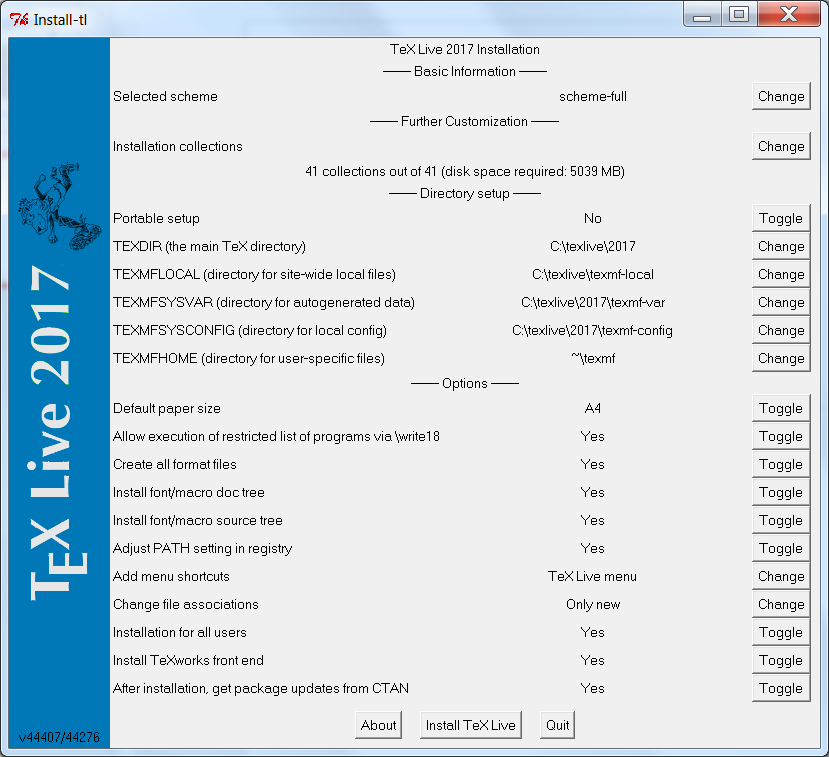
\includegraphics[width=.7\textwidth]{figs/texlive2017.png} 
\caption{پنجره‌ی نصب \lr{TeXLive 2017}.}
\end{figure}
	\chapter{راهنمای استفاده از قالب \texttt{vruthesis}}

برای \gls{typeset} پایان‌نامه‌ها و رساله‌های دانشکده‌ی علوم ریاضی، می‌توان از قالب \texttt{vruthesis} استفاده نمود. در این فصل، ابتدا در بخش \ref{sec:file_org} به سازمان \glspl{file}ی مورد استفاده در این قالب پرداخته می‌شود. شیوه‌ی قرارگیری جدول‌ها، شکل‌ها، نمودارها، الگوریتم‌ها و قطعه‌برنامه‌ها در بخش \ref{sec:figs_tbls_algs_codes} ذکر می‌شود. بخش \ref{sec:eqs} به \gls{typeset}ِ روابط ریاضی اختصاص دارد. نکات مربوط به فرهنگ‌واژگان و نمادها در بخش \ref{sec:gloss} ذکر شده‌اند. در پایان، بخش \ref{sec:faq}، برخی از نکات سودمند در استفاده از این قالب را گوشزد می‌کند.

\section{سازمان \glspl*{file}ی قالب \texttt{vruthesis}}\label{sec:file_org} 
	متن یک پایان‌نامه به طور معمول، یک متن طولانی است. بنابراین، بهتر است تنظیمات \gls{formatting} و محتوای پایان‌نامه را از یکدیگر جدا کنیم. تنظیمات \gls{formatting} در \gls{file} \texttt{vruthesis.cls} آمده است. علاوه بر این، به منظور مدیریت بهتر بر محتوا، محتوای پایان‌نامه نیز بر اساس فصل در \glspl{file}ی متعدد، تقسیم‌بندی شده‌اند. به منظور سادگی بیشتر، نمونه‌ی یک پایان‌نامه‌ی کارشناسی ارشد و نمونه‌ی یک رساله‌ی دکتر در \gls{site} دانشکده قرار گرفته‌اند. هر یک از این نمونه‌ها، شامل چند \gls{file} مختلف هستند. فهرست این \glspl{file} و کاربرد هر یک از آن‌ها در جدول \ref{tbl:fileList} آمده است. استفاده از دستوراتی که در شرح آن‌ها، عبارت «در صورت وجود» آمده است؛ اختیاری است و در صورتی که این دستورات در \gls{file} \verb|data.tex| نیامده باشند یا به صورت توضیح درج شده باشند؛ خروجی به صورت متناسب تولید می‌گردد.

\begin{table}[ht]
	\caption[\glspl*{file}ی موجود در نمونه‌ی پایان‌نامه دانشکده.]{فهرست و کاربرد \glspl*{file}ی موجود در نمونه‌ی پایان‌نامه‌ی دانشکده‌ی علوم ریاضی.}
	\label{tbl:fileList}
	\centering
	\begin{tabular}{| R{0.60\textwidth} | L{0.25\textwidth} |}
		\hline 
		\textbf{شرح} & \textbf{نام \gls{file}} \\
		\hline
		\glspl{file} اصلی پایان‌نامه، شامل ارجاع به تنظیمات، محتوا و سایر دستورات & \texttt{thesis.tex} \\ \hline
		قالب \texttt{vruthesis} & \texttt{vruthesis.cls} \\ \hline
		اطلاعات مربوط به صفحات ابتدایی و انتهایی پایان‌نامه مانند عنوان (لاتین)، چکیده (لاتین) و مانند آن & \texttt{data.tex} \\ \hline
		تعریف منابع و مآخذ به صورت \texttt{bibtex} &  \texttt{references.bib} \\ \hline
		\gls{formatting} مراجع مطابق با استاندارد \lr{IEEE} با تغییرات مصوب گروه علوم‌کامپیوتر &  \texttt{ieeetr-fa-vru.bst} \\ \hline
		\gls{formatting} مراجع مطابق با استاندارد \lr{ACM} با در نظر گرفتن مراجع فارسی &  \texttt{acm-fa.bst} \\ \hline
		محتویات مربوط به فصل \lr{X} پایان‌نامه &  \texttt{chapterX.tex} \\ \hline
		محتویات مربوط به پیوست \lr{X} پایان‌نامه &  \texttt{appendixX.tex} \\ \hline
		اطلاعات مورد نیاز برای ساخت فهرست واژگان & \texttt{gloss.tex} \\ \hline
		فهرست اختصارات و نمادها & \texttt{acronym.tex} \\ \hline
	\end{tabular}
\end{table}

	برای تولید \gls{file} نهایی پایان‌نامه در قالب \gls{pdf}، لازم است تا از موتور \lr{TeX Live 2017} استفاده شود. دستورات مورد نیاز برای تولید خروجی، در شکل \ref{fig:output_cmd} ذکر شده‌اند. 
	
	\begin{figure}
		\begin{latin}
\centering
	\begin{verbatim}
	xelatex -synctex=-1 thesis.tex
bibtex8 -W -c cp1256fa thesis
xindy -L persian-variant1 -C utf8 -I xindy -M thesis.xdy 
        -t thesis.glg -o thesis.gls thesis.glo
xindy -L persian-variant1 -C utf8 -I xindy -M thesis.xdy 
        -t thesis.blg -o thesis.bls thesis.blo
xindy -L english -C utf8 -I xindy -M thesis.xdy -t thesis.alg 
        -o thesis.acr thesis.acn
xelatex -synctex=-1 thesis.tex
xelatex -synctex=-1 thesis.tex
	\end{verbatim}
	\end{latin}
\caption{دستورات لازم برای تولید خروجی نهایی به قالب \gls*{pdf}.}
\label{fig:output_cmd}
\end{figure}

در پایان‌نامه‌ی نمونه، $5$ فصل و یک پیوست درنظر گرفته شده است. در صورتی که در پایان‌نامه‌ی خود، به فصل‌های (پیوست‌های) بیشتری نیاز دارید؛ می‌توانید با تهیه‌ی یک رونوشت از \gls{file} \texttt{chapterX.tex} (\texttt{appendixX.tex}) و ذخیره‌ی آن به نام دلخواه، فصل (پیوست) جدیدی را ایجاد کنید. لازم به ذکر است که برای لحاظ شدن فصل جدید در خروجی، نیاز است تا در \gls{file} \texttt{thesis.tex}، دستور
\begin{latin}
	\begin{verbatim}
	\include{chapterX}
	\end{verbatim}
\end{latin}
را پس از {\verb|\include{chapter5}|} یا آخرین فصل اضافه شده، قرار دهید. به طور مشابه، برای لحاظ شدن پیوست جدید در خروجی، لازم است تا دستور \verb|\include{appendixX}| پس از \verb|\include{appendix1}| قرار گیرد. 

	جهت تولید صفحات عنوان، ارزیابی، سپاسگزاری، تقدیم‌به و چکیده به هر دو زبان فارسی و انگلیسی، لازم است تا محتوای \gls{file} \texttt{data.tex} را به صورت مناسب، تکمیل کنید. دستورات مورد استفاده در این \gls{file} و کاربرد آن‌ها در جدول \ref{tbl:data_cmds} آمده‌اند. این دستورات ممکن است در نگاه اوّل گیج‌کننده به نظر برسند. به همین دلیل، توصیه می‌شود که از \gls{file} \verb|data.tex| در پایان‌نامه‌ی نمونه استفاده کرده و تنها محتویات خود را در آن، جایگزین نمایید. 
	
	\begin{longtable}[c]{| L{.45\textwidth} | R{.45\textwidth} |}
		\caption{دستورات قابل استفاده در \gls*{file} \texttt{thesis.tex}.}
	\label{tbl:data_cmds}
	\\
	\hline	
		\textbf{شرح} & \textbf{دستور} \\ \hline
	\endfirsthead
	\multicolumn{2}{c}{ادامه‌ی جدول \ref{tbl:data_cmds}.} \\ \hline
	\textbf{شرح} & \textbf{دستور} \\ \hline
	\endhead
		\multicolumn{2}{c}{ادامه‌ی جدول در صفحه‌ی بعد.} \\
	\endfoot
		\hline
	\multicolumn{2}{c}{پایان جدول \ref{tbl:data_cmds}.} \\ 
	\endlastfoot
	
		عنوان دانشکده به فارسی &  \verb|\faculty{}| \\ \hline
		عنوان دانشکده به انگلیسی &  \verb|\facultyen{}| \\ \hline
		نام گروه به فارسی &  \verb|\department{}| \\ \hline
		نام گروه به انگلیسی &  \verb|\departmenten{}| \\ \hline
		عنوان رشته‌ی تحصیلی به فارسی &  \verb|\subject{}| \\ \hline
		عنوان رشته‌ی تحصیلی به انگلیسی &  \verb|\subjecten{}| \\ \hline
		عنوان گرایش تحصیلی به فارسی &  \verb|\field{}| \\ \hline
		عنوان گرایش تحصیلی به انگلیسی &  \verb|\fielden{}| \\ \hline
		عنوان پایان‌نامه به فارسی &  \verb|\title{}| \\ \hline
		عنوان پایان‌نامه به انگلیسی &  \verb|\titleen{}| \\ \hline
		نام و نام خانوادگی استاد راهنما به فارسی با پیشوند «دکتر» &  \verb|\firstsupervisor{}| \\ \hline
		نام و نام خانوادگی استاد راهنما به انگلیسی با پیشوند «\lr{Dr.}» &  \verb|\firstsupervisoren{}| \\ \hline
		رتبه‌ی علمی استاد راهنما به فارسی &  \verb|\firstsupervisorrank{}| \\ \hline
		رتبه‌ی علمی استاد راهنما به انگلیسی &  \verb|\firstsupervisorranken{}| \\ \hline
		نام و نام خانوادگی استاد راهنمای دوم، در صورت وجود، به فارسی با پیشوند «دکتر» &  \verb|\secondsupervisor{}| \\ \hline
		نام و نام خانوادگی استاد راهنمای دوم، در صورت وجود، به انگلیسی با پیشوند «\lr{Dr.}» &  \verb|\secondsupervisoren{}| \\ \hline
		رتبه‌ی علمی استاد راهنمای دوم، در صورت وجود، به فارسی &  \verb|\secondsupervisorrank{}| \\ \hline
		رتبه‌ی علمی استاد راهنمای دوم، در صورت وجود، به انگلیسی &  \verb|\secondsupervisorranken{}| \\ \hline
		نام و نام خانوادگی استاد مشاور، در صورت وجود، به فارسی با پیشوند «دکتر» &  \verb|\firstadvisor{}| \\ \hline
		نام و نام خانوادگی استاد مشاور، در صورت وجود، به انگلیسی با پیشوند «\lr{Dr.}» &  \verb|\firstadvisoren{}| \\ \hline
		رتبه‌ی علمی استاد مشاور، در صورت وجود، به فارسی &  \verb|\firstadvisorrank{}| \\ \hline
		رتبه‌ی علمی استاد مشاور، در صورت وجود، به انگلیسی &  \verb|\firstadvisorranken{}| \\ \hline
		نام و نام خانوادگی استاد مشاور دوم، در صورت وجود، به فارسی با پیشوند «دکتر» &  \verb|\secondadvisor{}| \\ \hline
		نام و نام خانوادگی استاد مشاور دوم، در صورت وجود، به انگلیسی با پیشوند «\lr{Dr.}» &  \verb|\secondadvisoren{}| \\ \hline
		رتبه‌ی علمی استاد مشاور دوم، در صورت وجود، به فارسی &  \verb|\secondadvisorrank{}| \\ \hline
		رتبه‌ی علمی استاد مشاور دوم، در صورت وجود، به انگلیسی &  \verb|\secondadvisorranken{}| \\ \hline
		نام و نام خانوادگی استاد داور داخلی اول به فارسی با پیشوند «دکتر» &  \verb|\firstinternalreferee{}| \\ \hline
		نام و نام خانوادگی استاد داور داخلی اول به انگلیسی با پیشوند «\lr{Dr.}» &  \verb|\firstinternalrefereeen{}| \\ \hline
		رتبه‌ی علمی استاد داور داخلی اول به فارسی &  \verb|\firstinternalrefereerank{}| \\ \hline
		رتبه‌ی علمی استاد داور داخلی اول به انگلیسی &  \verb|\firstinternalrefereeranken{}| \\ \hline
		نام و نام خانوادگی استاد داور داخلی دوم، در صورت وجود، به فارسی با پیشوند «دکتر» &  \verb|\secondinternalreferee{}| \\ \hline
		نام و نام خانوادگی استاد داور داخلی دوم، در صورت وجود، به انگلیسی با پیشوند «\lr{Dr.}» &  \verb|\secondinternalrefereeen{}| \\ \hline
		رتبه‌ی علمی استاد داور داخلی دوم، در صورت وجود، به فارسی &  \verb|\secondinternalrefereerank{}| \\ \hline
		رتبه‌ی علمی استاد داور داخلی دوم، در صورت وجود، به انگلیسی &  \verb|\secondinternalrefereeranken{}| \\ \hline
		نام و نام خانوادگی استاد داور خارجی اول به فارسی با پیشوند «دکتر» &  \verb|\firstexternalreferee{}| \\ \hline
		نام و نام خانوادگی استاد داور خارجی اول به انگلیسی با پیشوند «\lr{Dr.}» &  \verb|\firstexternalrefereeen{}| \\ \hline
		رتبه‌ی علمی استاد داور خارجی اول به فارسی &  \verb|\firstexternalrefereerank{}| \\ \hline
		رتبه‌ی علمی استاد داور خارجی اول به انگلیسی &  \verb|\firstexternalrefereeranken{}| \\ \hline
		نام و نام خانوادگی استاد داور خارجی دوم، در صورت وجود، به فارسی با پیشوند «دکتر» &  \verb|\secondexternalreferee{}| \\ \hline
		نام و نام خانوادگی استاد داور خارجی دوم، در صورت وجود، به انگلیسی با پیشوند «\lr{Dr.}» &  \verb|\secondexternalrefereeen{}| \\ \hline
		رتبه‌ی علمی استاد داور خارجی دوم، در صورت وجود، به فارسی &  \verb|\secondexternalrefereerank{}| \\ \hline
		رتبه‌ی علمی استاد داور خارجی دوم، در صورت وجود، به انگلیسی &  \verb|\secondexternalrefereeranken{}| \\ \hline
		نام و نام خانوادگی استاد ناظر به فارسی با پیشوند «دکتر» &  \verb|\viewer{}| \\ \hline
		نام و نام خانوادگی استاد ناظر به انگلیسی با پیشوند «\lr{Dr.}» &  \verb|\vieweren{}| \\ \hline
		رتبه‌ی علمی استاد ناظر به فارسی &  \verb|\viewerrank{}| \\ \hline
		رتبه‌ی علمی استاد ناظر به انگلیسی &  \verb|\viewerranken{}| \\ \hline
		نام دانشجو به فارسی &  \verb|\name{}| \\ \hline
		نام دانشجو به انگلیسی &  \verb|\nameen{}| \\ \hline
		نام خانوادگی دانشجو به فارسی &  \verb|\surname{}| \\ \hline
		نام خانوادگی دانشجو به انگلیسی &  \verb|\surnameen{}| \\ \hline
		ماه و سال جلسه‌ی دفاع به تقویم شمسی، مانند آذر $1396$ &  \verb|\thesisdate{}| \\ \hline
		ماه و سال جلسه‌ی دفاع به تقویم میلادی، مانند \lr{December 2017} &  \verb|\thesisdateen{}| \\ \hline
		تعداد واحد پایان‌نامه به فارسی، مانند $6$ &  \verb|\credit{}| \\ \hline
		تعداد واحد پایان‌نامه به انگلیسی، مانند \lr{$6$} &  \verb|\crediten{}| \\ \hline
		تاریخ جلسه‌ی دفاع به تقویم شمسی، مانند $۱۳۹۶/۰۹/۳۰$ &  \verb|\defensedate{}| \\ \hline
		تاریخ جلسه‌ی دفاع به تقویم میلادی، مانند \lr{December 21${}^{\text{st}}$, 2017}  &  \verb|\defensedateen{}| \\ \hline
		نمره‌ی پایان‌نامه با اعداد فارسی مانند، $19.75$ &  \verb|\grade{}| \\ \hline
		نمره‌ی پایان‌نامه با اعداد انگلیسی مانند، \lr{$19.75$} &  \verb|\gradeen{}| \\ \hline
		نمره‌ی پایان‌نامه به حروف به زبان فارسی &  \verb|\letgrade{}| \\ \hline
		نمره‌ی پایان‌نامه به حروف به زبان انگلیسی  &  \verb|\letgradeen{}| \\ \hline
		درجه‌ی دفاع به فارسی &  \verb|\degree{}| \\ \hline
		درجه‌ی دفاع به انگلیسی &  \verb|\degreeen{}| \\ \hline
		متن تقدیم‌به به زبان فارسی &  \verb|\totext{}| \\ \hline
		متن سپاسگزاری به فارسی &  \verb|\ack{}| \\ \hline
		متن چکیده به فارسی &  \verb|\abstractfa{}| \\ \hline
		متن چکیده به انگلیسی &  \verb|\abstracten{}| \\ \hline
	\end{longtable}

		\section{درج جدول‌ها، شکل‌ها، نمودارها، الگوریتم‌ها و قطعه‌برنامه‌ها}\label{sec:figs_tbls_algs_codes}
		پایان‌نامه‌ی شما ممکن است دارای جدول‌ها، شکل‌ها، نمودارها، الگوریتم‌ها و قطعه‌برنامه‌های مختلفی باشد. در این قالب، سه نوع محتوا درنظر گرفته شده است:
		\begin{itemize}
			\item جدول که تنها برای نمایش جدول‌ها استفاده می‌شود.
				\item الگوریتم که تنها برای نمایش الگوریتم‌ها استفاده می‌شود. 
			\item شکل که برای نمایش نمودارها،  قطعه‌برنامه‌ها، \glspl{flowchart} و سایر موارد بصری مورد استفاده قرار می‌گیرد.
		\end{itemize}
		
		در ادامه، نمونه‌ای از هر یک از موارد فوق آمده است. جدول \ref{tbl1}، یک جدول با تعداد ستون‌های زیاد است که لازم است تا در صفحه‌ای جداگانه درج شود. قطعه کد تولیدکننده‌ی این جدول در شکل \ref{fig:tbl1} آمده است. 
		
			شکل \ref{fig:clus1} نمونه‌ای از یک خوشه‌بندی برای یک دادگان نمونه است. همچنین، الگوریتم \ref{fig:alg} نیز نمونه‌ای از یک الگوریتم را نشان می‌دهد. از شکل‌ها می‌توان به منظور نمایش نمودارها نیز استفاده کرد؛ مانند \ref{fig:chart}. همچنین، شکل \ref{fig:tbl1}، بیانگر یک قطعه‌کد در \lr{\LaTeX} است. 
			
			\begin{figure}
				\centering
				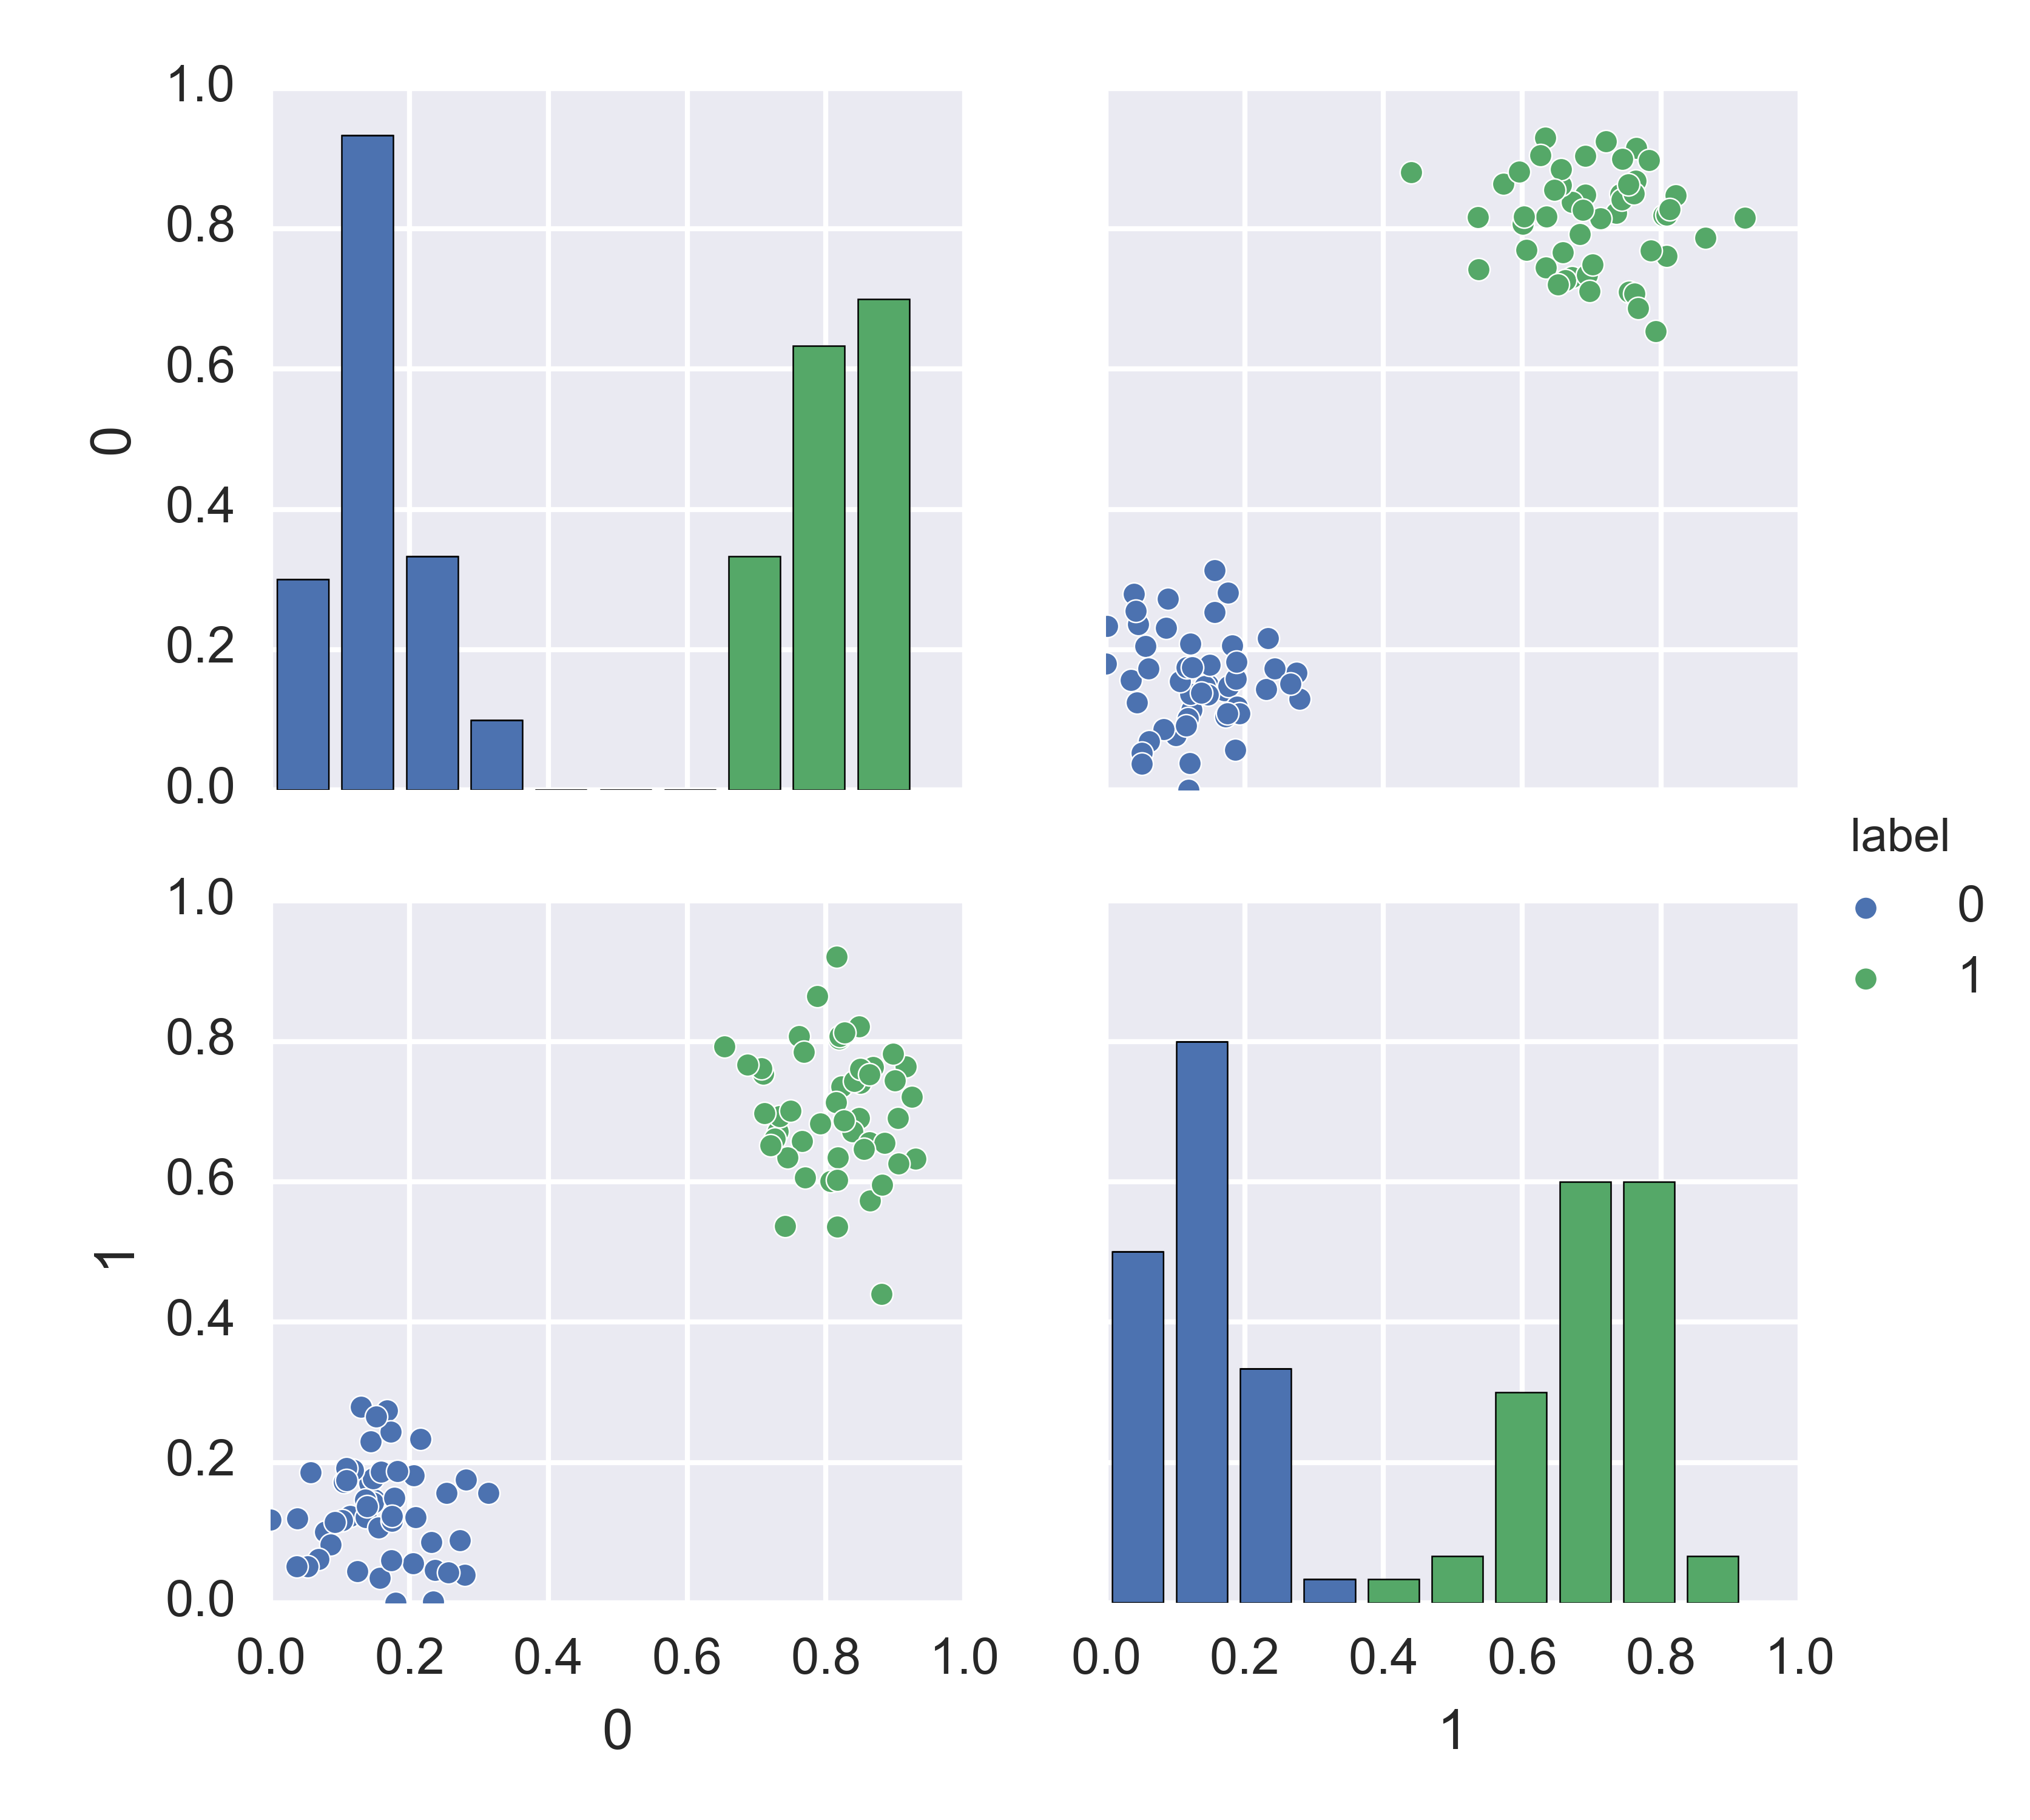
\includegraphics[width=.7\textwidth]{clus1}
				\caption{نمونه‌ای از یک خوشه‌بندی برای یک دادگان نمونه.}
				\label{fig:clus1}
			\end{figure}
		
		\begin{algorithm}
				\begin{latin}
		\begin{algorithmic}[1] % The number tells where the line numbering should start
        \Procedure{Euclid}{$a,b$} \Comment{\rl{ب.م.م. دو عدد صحیح مثبت $a$ و $b$}}
            \State $r\gets a \bmod b$
            \While{$r\not=0$} \Comment{\rl{اگر $r$ صفر باشد؛ پاسخ محاسبه شده است.}}
                \State $a \gets b$
                \State $b \gets r$
                \State $r \gets a \bmod b$
            \EndWhile\label{euclidendwhile}
            \State \textbf{return} $b$\Comment{\rl{ب.م.م. برابر با $b$ است.}}
        \EndProcedure
    \end{algorithmic}
    \end{latin}
    		\caption{الگوریتم اقلیدس برای محاسبه‌ی \gls*{gcd}.}
				\label{fig:alg}		
		\end{algorithm}	
			
			\begin{figure}
				\centering
				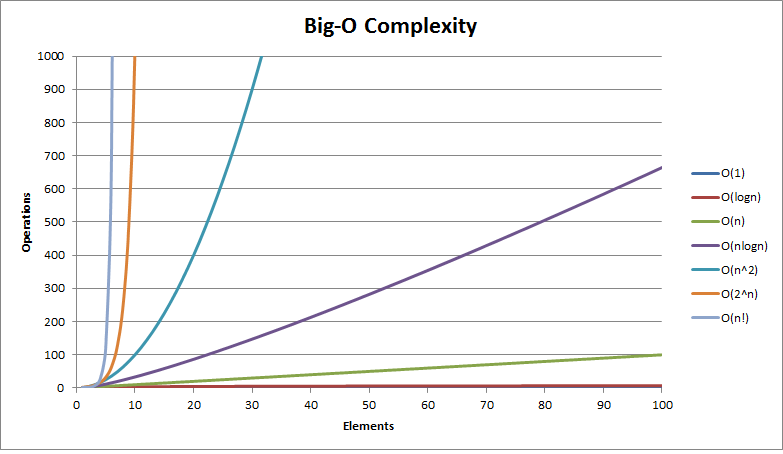
\includegraphics[width=.7\textwidth]{chart}
				\caption{نمونه‌ای از یک نمودار.}
				\label{fig:chart}
			\end{figure}
		
		\begin{figure}
			\centering
		\footnotesize
		\begin{myverbatim}
\begin{landscape}
  \begin{table}
    \caption{+rl[نمونه‌ای از یک جدول با تعداد ستون‌های زیاد.]}
    \label{tbl1}
    \centering
    \footnotesize
    \begin{tabular}{|r||c|c|c|c|c|c|c|c|c|c|c|c|c|c|c|}
      \hline
      \textbf{+rl[عنوان]} & $\alpha$ 
        & \multicolumn{5}{|c|}{$\gamma_1, \gamma_2, \ldots, \gamma_5$} 
        & $\beta$ & \multicolumn{8}{|c|}{+rl[سایر پارامترها]} \\ \hline
      +rl[نمونه‌ی اول]   &   74.85 &  0.32 &  13.99 &  91.25 &  80.74
         &  15.44 &  74.49 &  42.13 &
        1.08  &  32.98 &  18.74 &  46.83 &  81.28 &  31.52 &  8.29 \\
      +rl[نمونه‌ی دوم] &   22.76 &  48.61 &  
        70.77 &  22.77 &  3.81 &  45.05 &  
        70.55 &  33.20 &  1.40  &  24.42 &  79.06 &  
          30.38 &  24.95 &  19.77 &  44.59 \\
      +rl[نمونه‌ی سوم] &   55.67 &  36.98 &
          89.61 &  56.43 &  88.97 &  38.21 &  
        81.40 &  77.05 &  9.35 &  18.52 &  3.48 &  
          95.93 &  9.20 &  16.30 &  84.36 \\
      +rl[نمونه‌ی چهارم] &   60.31 &  88.25 &
          29.96 &  56.83 &  89.49 &  38.26 &  
        55.73 &  99.36 &  21.70 &  74.46 &  49.11 &  2.82
           &  25.47 &  2.90 &  84.58 \\
      +rl[نمونه‌ی پنجم] &   90.17 &  51.53 
        &  32.67 &  82.55 &  87.72 &  66.09 &  26.86 &  
        4.69 &  77.97 &  40.23 &  58.59 &  70.13 &  70.23 &
            80.73 &  64.88 \\
      +rl[نمونه‌ی ششم] &   74.92 
        &  52.33 &  98.68 &  63.75 &  30.10 &  7.32 &  91.70 &  
        72.76 &  42.50 &  26.72 &  23.33 &  73.55 & 
           77.37 &  32.79 &  15.60 \\
      +rl[نمونه‌ی هفتم] &   26.85 &  55.27
         &  5.12 &  88.21 &  4.92 &  70.78 &  
        75.26 &  32.03 &  25.11 &  61.81 &  44.24 &
            47.14 &  98.98 &  16.90 &  20.27 \\
      +rl[نمونه‌ی هشتم] &   84.33 &  12.53 &  36.00
         &  24.02 &  44.60 &  8.44 &  
        5.73 &  10.37 &  16.94 &  15.41 &  39.69 &
            43.74 &  10.43 &  73.96 &  26.51 \\
      +rl[نمونه‌ی نهم] &   59.21 &  47.46 & 
           97.27 &  87.05 &  84.65 &  17.95 &  50.05 &  
        38.68 &  20.09 &  46.99 &  12.47 &  10.92 & 
           78.38 &  74.53 &  31.83 \\
      +rl[نمونه‌ی دهم] &   97.61 &  33.47 &  67.78 
        &  69.95 &  60.95 &  88.40 &  
        59.64 &  18.22 &  57.49 &  97.76 &  40.31 &
            4.83 &  8.90 &  69.18 &  97.02 \\ \hline
    \end{tabular}
  \end{table}
\end{landscape}
		\end{myverbatim}
		\caption{قطعه‌کد مربوط به تولید جدول \ref{tbl1}.}
		\label{fig:tbl1}
		\end{figure}
	
	
		
		\begin{landscape}
			\begin{table}
				\caption{نمونه‌ای از یک جدول با تعداد ستون‌های زیاد.}
				\label{tbl1}
				\centering
				\footnotesize
				\begin{tabular}{|r||c|c|c|c|c|c|c|c|c|c|c|c|c|c|c|}
				\hline
				\textbf{عنوان} & $\alpha$ & \multicolumn{5}{|c|}{$\gamma_1, \gamma_2, \ldots, \gamma_5$} & $\beta$ & \multicolumn{8}{|c|}{سایر پارامترها} \\ \hline
نمونه‌ی اول 	&   74.85 &  0.32 &  13.99 &  91.25 &  80.74 &  15.44 &  74.49 &  42.13 &  1.08  &  32.98 &  18.74 &  46.83 &  81.28 &  31.52 &  8.29 \\
نمونه‌ی دوم &   22.76 &  48.61 &  70.77 &  22.77 &  3.81 &  45.05 &  70.55 &  33.20 &  1.40  &  24.42 &  79.06 &  30.38 &  24.95 &  19.77 &  44.59 \\
نمونه‌ی سوم &   55.67 &  36.98 &  89.61 &  56.43 &  88.97 &  38.21 &  81.40 &  77.05 &  9.35 &  18.52 &  3.48 &  95.93 &  9.20 &  16.30 &  84.36 \\
نمونه‌ی چهارم &   60.31 &  88.25 &  29.96 &  56.83 &  89.49 &  38.26 &  55.73 &  99.36 &  21.70 &  74.46 &  49.11 &  2.82 &  25.47 &  2.90 &  84.58 \\
نمونه‌ی پنجم &   90.17 &  51.53 &  32.67 &  82.55 &  87.72 &  66.09 &  26.86 &  4.69 &  77.97 &  40.23 &  58.59 &  70.13 &  70.23 &  80.73 &  64.88 \\
نمونه‌ی ششم &   74.92 &  52.33 &  98.68 &  63.75 &  30.10 &  7.32 &  91.70 &  72.76 &  42.50 &  26.72 &  23.33 &  73.55 &  77.37 &  32.79 &  15.60 \\
نمونه‌ی هفتم &   26.85 &  55.27 &  5.12 &  88.21 &  4.92 &  70.78 &  75.26 &  32.03 &  25.11 &  61.81 &  44.24 &  47.14 &  98.98 &  16.90 &  20.27 \\
نمونه‌ی هشتم &   84.33 &  12.53 &  36.00 &  24.02 &  44.60 &  8.44 &  5.73 &  10.37 &  16.94 &  15.41 &  39.69 &  43.74 &  10.43 &  73.96 &  26.51 \\
نمونه‌ی نهم &   59.21 &  47.46 &  97.27 &  87.05 &  84.65 &  17.95 &  50.05 &  38.68 &  20.09 &  46.99 &  12.47 &  10.92 &  78.38 &  74.53 &  31.83 \\
نمونه‌ی دهم &   97.61 &  33.47 &  67.78 &  69.95 &  60.95 &  88.40 &  59.64 &  18.22 &  57.49 &  97.76 &  40.31 &  4.83 &  8.90 &  69.18 &  97.02 \\ \hline
				\end{tabular}
			\end{table}
		\end{landscape}
	
		\section{روابط ریاضی}\label{sec:eqs}
		به طور معمول، بخش زیادی از یک پایان‌نامه در دانشکده‌ی علوم ریاضی، از روابط ریاضی تشکیل شده است. یک رابطه‌ی ریاضی را می‌توان به صورت \gls{inline} مانند $\int_{-\infty}^{+\infty} \sin x \mathrm{d} x$ نوشت. همچنین، می‌توان یک رابطه‌ی ریاضی را بدون شماره‌گذاری مانند
		$$
			A \wedge \left( B \vee C \right) = \left(A \wedge B \right) \vee \left( A \wedge C \right),
		$$
		نوشت. امّا، با توجه به زیادبودن تعداد روابط ریاضی، بهتر است در صورتی که به یک رابطه ارجاع داده می‌شود؛ آن را شماره‌گذاری نمایید؛ مانند
		\begin{equation}
			P \left(B_i \vert A \right) = \frac{P\left(A \vert B_i \right) P\left(B_i\right)}{\sum_j P\left(A \vert B_j \right) P\left(B_j\right)},
			\label{eq:1}
		\end{equation}
		که $i=1,\ldots,k$ است. بنابراین، می‌توان به سادگی به رابطه‌ی \ref{eq:1}، ارجاع داد. 
		
		همچنین، محیط‌های متنوعی برای \gls{typeset} قضیه‌ها، لم‌ها، گزاره‌ها، نتیجه‌ها، تعریف‌ها و مانند آن‌ها در نظر گرفته شده‌اند که در ادامه، نمونه‌های مختلفی از آن‌ها را مشاهده می‌کنید.
		
		\begin{theorem}[\cite{gary}]
			\label{}
			زبان $\mathrm{SAT} = \left\{ \left\langle \Phi \right\rangle \ \vert \ \text{\rl{ صدق‌پذیر است} } \Phi  \right\}$، مفروض است. داریم
			\begin{equation}
				\mathrm{SAT} \in \mathbf{NP}\mathrm{-complete}.
			\end{equation}
		\end{theorem}
		\begin{proof}
			برای اثبات می‌توان به مرجع \cite{gary} مراجعه نمود. 
		\end{proof}
		
		\begin{definition}[ضخامت گراف]
			ضخامت گراف $G$ عبارت است از حداقل تعداد گراف‌های مسطح ممکن در تجزیه‌ی $G$ به گراف‌های مسطح.
		\end{definition}
		
		\begin{lemma}{قضیه‌ی پنج رنگ \cite{heawood1890}}
			هر گراف مسطح، قابل $5$-رنگ‌آمیزی است.
		\end{lemma}
		
		\begin{conjecture}[سلام این یک متن است.\cite{ringel1964}]
			درخت $T$ با $m$ یال مفروض است. در این صورت، $K_{2m+1}$ قابل تجزیه به $2m+1$ کپی از $T$ است.
		\end{conjecture}
		
		\begin{problem}
			\gls{bandwidth} گراف $K_{n_1 \ldots n_k}$ را محاسبه نمایید.
		\end{problem}
		
		\begin{proposition}
			ضخامت گراف ساده‌ی $G$ از مرتبه‌ی $n$ و اندازه‌ی $m$، حداقل برابر است با $\frac{m}{3n-6}$.
		\end{proposition}
		
		\begin{corollary}
اندازه‌ی \gls{smallest} و \gls{lmatch} در گراف‌های دوبخشی با یکدیگر برابر است.
		\end{corollary}
		
		\begin{remark}
			نمونه‌های مربوط به گزاره‌ها، قضیه‌ها، تعریف‌ها و مانند آن‌ها در این بخش از مرجع \cite{west} اخذ شده‌اند.
		\end{remark}
		
		\begin{example}
			مثال‌های زیادی از مسائل $\mathbf{NP}\mathrm{-complete}$ وجود دارند؛ مانند $\mathrm{CLIQUE}$.
		\end{example}		
		\section{فرهنگ‌واژگان و نمادها}\label{sec:gloss}
		جهت استفاده از فرهنگ واژگان و نمادها و اختصارات، می‌توانید از دستورات مرتبط استفاده نمایید. قابل ذکر است که قبل از استفاده از یک اختصار یا یک واژه، لازم است تا آن را در یکی از \glspl{file}ی \lr{acronym.tex} یا \lr{gloss.tex} تعریف کنید. در صورتی که واژه یا نماد را به شکل \gls{file} \lr{acronym.tex} تعریف کنید؛ آن واژه در فهرست نماد‌ها و اختصارات درج خواهد شد. همچنین، در صورتی که واژه به شکل \gls{file} \lr{gloss.tex} تعریف شود؛ واژه در فرهنگ واژگان قرار می‌گیرد.
		
		این راهنما به زودی تکمیل می‌گردد.
		\section{برخی نکات سودمند}\label{sec:faq}
			جهت قرارگرفتن تمام مدخل‌های \gls{file} \lr{\texttt{references.bib}}\cite{*} در فهرست مراجع.
	
	\chapter[راهنمای استفاده از قالب \lr{\texttt{vruthesis}} جهت نگارش]{راهنمای استفاده از قالب  جهت نگارش پایان‌نامه‌های دانشگاه ولی‌عصر (عج) رفسنجان}
	در این فصل، گزیده‌ای از «راهنمای استفاده از قالب \lr{\texttt{vruthesis}} جهت نگارش پایان‌نامه/رساله‌های دانشگاه ولی‌عصر (عج) رفسنجان» به نقل از \cite{vru_grad_rules} ذکر می‌گردد. لازم به ذکر است که دستورات مربوط به قالب‌بندی، در این نمونه به صورت دقیق رعایت شده و به تایید شورای تحصیلات تکمیلی دانشکده‌ی ریاضی رسیده است. بنابراین، در صورتی که از این نمونه برای آماده‌سازی پایان‌نامه‌ی خود استفاده می‌کنید؛ نیاز به انجام کار خاصی ندارید.
	\section{چگونگی تنظیم مطالب پایان‌نامه}
		\begin{enumerate}
			\item برگ نخست: سفید
			\item برگ دوم: بسم اللّه الرحمن الرحیم (در وسط صفحه)
			\item برگ سوم: مطابق شکل \ref{app1}
			\item برگ چهارم: تصویب‌نامه‌ی پایان‌نامه به همراه امضای استادان راهنما، مشاور، داور و نماینده‌ی تحصیلات تکمیلی، مطابق با شکل \ref{app2}
			\item پشت برگ چهارم: شکل \ref{app4}
			\item برگ پنجم: سپاس‌گزاری (اختیاری)
			\item پشت برگ پنجم: تقدیم اثر (اختیاری)
			\item مخفف‌ها یا کوتاه‌نوشت‌ها  (در صورت لزوم)
			\item چکیده که شامل هدف، روش پژوهش، نتایج به‌دست آمده و راهکار‌های پیشنهادی برای پژوهش‌های آتی می‌باشد و باید حداقل $200$ کلمه و در یك صفحه و یک پاراگراف، بدون ذکر منابع و شكل باشد. 
			\item فهرست: به‌ترتیب باید فهرست مطالب، شکل‌ها و جدول‌ها ارایه شوند (مطابق با شکل \ref{app5}).
			\item مقدمه (فصل اول): در این قسمت به معرفی پایان‌نامه، فرضیه‌ها و اهداف پژوهش پرداخته می‌شود. (حداکثر در $5$ صفحه).
			\item متن اصلی پایان‌نامه شامل: پیشینه‌ی پژوهش (فصل دوم)، مواد و روش‌ها (فصل سوم)، نتایج و بحث (فصل چهارم) و نتیجه‌گیری کلی و پیشنهادها (فصل پنجم) می‌باشد.
			\item پیوست‌ها: (در صورت وجود)
			\item منابع مورد استفاده: شیوه‌ی نوشتن منابع، مطابق با نمونه‌ی پیشنهادی در پیوست‌ \ref{app7} می‌باشد.
			\item چکیده‌ی انگلیسی: کاملاً منطبق با چکیده‌ی فارسی باشد و به صورت برعکس (از سمت چپ) صحافی شود.
			\item دو برگ ماقبل آخر: مطابق شکل‌های \ref{app3} و \ref{app6} باشند (به‌صورت برعکس صحافی شود)
			\item برگ آخر: صفحه‌ی سفید
		\end{enumerate}
		
		\begin{remark}
			توجه به نکات زیر، حائز اهمیت است:
			\begin{itemize}
				\item در تدوین‌ و تایپ‌ صفحات‌ پایان‌نامه‌ از هیچگونه‌ كادر تزئینی‌ و تذهیب‌ استفاده‌ نگردد.
				\item برای جداسازی فصل‌ها از \lr{break section} استفاده شود تا تمام فصول پشت سر هم در یک فایل موجود باشند. 
				\item پس از اتمام مرحله‌ی حروفچینی و صفحه‌آرایی، متن پایان‌نامه را به‌صورت \gls{pdf} در آورید.
				\item فرمول‌ها به‌صورت ایتالیک تایپ شوند.
			\end{itemize}
		\end{remark}

	\section{مشخصات سر صفحه}
			لازم است در بالای صفحات فرد، عنوان فصل در حاشیه‌ی سمت راست و شماره‌ی صفحه در حاشیه‌ی سمت چپ تایپ شود و در صفحات زوج، عنوان پایان‌نامه در حاشیه‌ی سمت چپ و شماره‌ی صفحه در حاشیه‌ی سمت راست درج شود (مطابق شکل \ref{fig:header}). 
	\begin{figure}
	\centering
	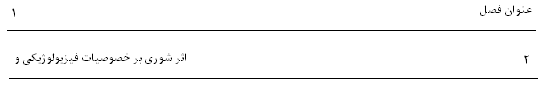
\includegraphics[width=.6\textwidth]{pages.png}
\caption{نمونه‌ای از شیوه‌ی صحیح قرارگیری مشخصات سرصفحه.}
\label{fig:header}
\end{figure}
			\begin{enumerate}[label=\Alph*:]
				\item سرصفحه (\lr{Header}) از صفحه‌ی دوم فصل اول شروع میشود و در صفحه‌ی اول هر فصل، قسمت سرصفحه حذف می‌شود. اول هر فصل باید \lr{break section} در بخش \lr{Page layout} استفاده شود تا سر فصل حذف شود و برای تکرار نشدن سرفصل‌ها در فصل‌های قبلی باید \lr{Link to previous} در بخش \lr{Design} استفاده شود.
				\item متن سرصفحه و شماره‌ی صفحه با قلم  \lr{BNazanin 12 Bold} نوشته شود. 
				\item صفحات سفید، سرصفحه ندارند. 
				\item صفحه‌ی اول فصل، پیوست، نمایه‌ها و واژه‌نامه، سرصفحه ندارند. 
				\item از صفحه‌ی فهرست تا شروع فصل اول، تمامی صفحات با حروف الفبای فارسی و در بالای صفحه، گوشه‌ی خارجی صفحه و به فاصله‌ی 5 سانتی‌متر از بالای كاغذ شماره‌گذاری ‌شود.
				\item از اولین صفحه‌ی فصل اول تا انتهای منابع، تمامی صفحات با اعداد1، 2، 3، و ... در بالای صفحه، گوشه‌ی خارجی صفحه و به فاصله‌ی 5 سانتی‌متر از بالای كاغذ شماره‌گذاری ‌شود.
			\end{enumerate}
			
		\section{نحوه‌ی نگارش}
			نرم‌افزار مورد استفاده برای نگارش پایان‌نامه،  \lr{Microsoft Word 2003} به بالا یا نرم‌افزار مناسب دیگر به تأیید كمیته‌ی تحصیلات تكمیلی دانشکده مربوطه می‌باشد. در صورت استفاده از برنامه \lr{Word}، توجه به نكات زیر ضروری است:  
			\begin{enumerate}%[label=\Alph*:]
				\item متن چکیده‌ی فارسی با قلم \lr{BNazanin 12} و کلمه «چکیده» در اولین خط با قلم \lr{BNazanin 12 Bold} در اول سطر درج شود. 
				\item متن چکیده‌ی انگلیسی با قلم \lr{Times New Roman 11} و کلمه \lr{Abstract} در اولین خط با قلم \lr{Time New Roman 11 Bold} در اول سطر درج شود. 
				\item متن مقدمه با قلم \lr{BNazanin 12} و کلمه «مقدمه» در اولین خط با قلم \lr{Bold  BNazanin 14} در اول سطر درج شود.
				\item متن اصلی پایان‌نامه باید روی دو طرف کاغذ \lr{A4} با قلم \lr{BNazanin 12} و با فاصله خطوط یکسان به صورت (\lr{Single}) نوشته شود. 
				\item در متن اصلی پایان‌نامه، لغات یا حروف انگلیسی (از جمله، منابع انگلیسی) با قلم \lr{Times New Roman 11} نوشته شود.
				\item عناوین فصل‌ها با قلم \lr{14 BNazanin Bold} نوشته شود.
				\item سطر اول تمامی پاراگراف‌های موجود در متن پایان‌نامه، بایستی $0.5$ سانتی‌متر تورفتگی داشته باشند. توجه داشته باشید که عنوان بخش‌ها یا زیر بخش‌ها نبایستی دارای تورفتگی باشند.
				\item قسمت‌های مختلف هر فصل با اعدادی نظیر 6-4- یا 6-4-2- مشخص میشود كه عدد 6 شماره‌ی فصل، عدد4 شماره‌ی بخش و عدد 2 شماره‌ی زیر بخش است. بخش‌های مختلف فصل‌ها با قلم \lr{BNazanin 13 Bold} و زیربخش‌های اول با قلم \lr{BNazanin 12 Bold}  و زیربخش‌های دوم با \lr{BNazanin 11 Bold} تایپ شود.
				\item تمامی شکل‌ها و جدول‌ها باید به ترتیب ظهور در هر فصل شماره‌گذاری شوند. مثلاً برای جدول‌های فصل 2، جدول 2-1، جدول 2-2 و ... برای جدول‌های فصل 3، جدول 3-1، جدول 3-2 و .... عنوان جدول‌ها در بالای آن‌ها و وسط صفحه و عنوان شکل‌ها در زیر آنها، وسط صفحه با قلم \lr{BNazanin 10 Bold}  نوشته شود. اعداد و متن داخل جدول با قلم \lr{BNazanin 10}   نوشته شود. اگر شکلی از مرجعی نقل شده باشد، لازم است مرجع آن در زیر شکل داخل پرانتز آورده شود.
				\item جدول‌هایی که در راستای طولی کاغذ تنظیم میشوند، باید طوری قرار گیرند که متن بالای آنها در سمت لبه‌ی پایان‌نامه واقع شود (درتمامی جدول‌ها خطوط عمودی باید حذف شود). شکل‌ها و جدول‌ها داخل متن و در نزدیکترین فاصله به محل ذکر شده، آورده شوند (حاشیه‌ی شکل‌ها حذف شود). هم‌چنین شکل‌هایی که در راستای طولی کاغذ تنظیم می‌شوند، باید طوری قرار گیرند که متن پایین آنها در سمت لبه‌ی پایان‌نامه قرار گیرد. 
				\item فرمول‌ها (در صورت نیاز به ارجاع) در هر فصل به‌طور جداگانه و به ترتیبی که ظاهر می‌شوند (مانند جدول‌ها و شکل‌ها) شماره‌گذاری می‌گردد (مانند 2-3، 2-4، 3-1 و ...).
				\item معادل انگلیسی لغات یا اصطلاحات فارسی که برای اولین‌بار به کار می‌رود به صورت زیرنویس (فقط برای یک‌بار) با قلم Times New Roman 10 در صفحه‌ی مربوط درج شود. (سعی شود در متن پایان‌نامه‌، از بکار بردن واژه‌های با الفبای انگلیسی خودداری شود). زیرنویس‌ها در هر صفحه با گذاردن شماره‌ی 1، 2 و ... در گوشه‌ی بالای آخرین کلمه در متن مشخص میشوند. زیر نویس باید به شکل زیر در زیر نویس آورده شود. \\
\begin{latin}
\footnotesize	$1$ Water use efficiency
\end{latin}
				\item لازم است در متن به تمامی منابعی كه مورد استفاده قرار می‌گیرند، اشاره شود. چنانچه در داخل متن از یك منبع مطلبی نقل شود، بلافاصله پس از ذكر نام نویسنده و یا در خاتمه‌ی جمله، پرانتزی باز شود و مرجع ذكر گردد. شیوه‌ی نامه‌ی نگارش منابع پیوست شده است (پیوست شماره‌ی \ref{app6}).
				
			\end{enumerate}

		حاشیه‌های صفحات مطابق نمونه‌ی شکل \ref{layout} ($4.5$ سانتیمتر فاصله از بالا و پایین و $4$ سانتیمتر از چپ و $5$ سانتیمتر از راست رعایت گردد (توجه: برای تنظیم این فاصله‌ها از حاشیه از طریق \lr{Page layout} وارد \lr{Page setup} شده و اعداد را با واحد سانتیمتر وارد کنید. در ضمن در همان صفحه در قسمت \lr{Multiple pages} کلمه \lr{mirror margin} را انتخاب کنید تا در صفحات زوج و فرد فاصله متن از حاشیه بیرونی $4$ سانتیمتر و از حاشیه درونی $5$ سانتیمتر شود (در \lr{Page setup} باید سایز (\lr{Size Letter}) انتخاب شود).
		
		\begin{figure}
	\centering
	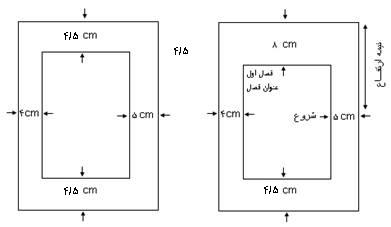
\includegraphics[width=.6\textwidth]{layout.png}
\caption{حاشیه‌ی صفحات.}
\label{layout}
\end{figure}
\section{نحوه‌ی صحافی پایان‌نامه}
	روی جلد مطابق یا پیوست شماره‌ی \ref{app1} تنظیم گردد، عطف آن مانند نمونه‌ی شکل \ref{atf} نوشته می‌شود.
	\begin{figure}
	\centering
	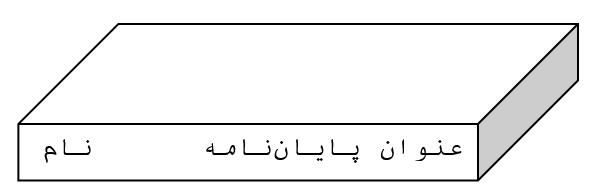
\includegraphics[width=.6\textwidth]{atf.png}
\caption{نمونه‌ای از شیوه‌ی صحیح \gls*{typeset} عطف.}
\label{atf}
\end{figure}
ابعاد پایان نامه بعد از صحافی، $23.5 \times 17$ (قطع وزیری) باید باشد. ابعاد سیاهه متن پایان‌نامه (از بالای متن سرصفحه تا پایین متن اصلی و عرض متن) $18.3 \times 12$ باید باشد. 
فاصله‌ی متن سرصفحه از حاشیه‌ی بالا $2.5$ سانتیمتر و فاصله‌ی متن اصلی از حاشیه‌ی پایین $2.7$ سانتیمتر، فاصله‌ی متن از حاشیه‌ی بیرونی $2$ سانتیمتر و از حاشیه‌ی درونی $3$ سانتیمتر باید باشد.  

رنگ جلد پایان‌نامه‌های کارشناسی‌ارشد کلیه رشته‌ها سورمه‌ای و رساله دکتری سبز یشمی می‌باشد. همچنین، اصل پایان‌نامه قبل از صحافی و پس از تایپ و آماده‌سازی به رؤیت مدیر تحصیلات تكمیلی دانشگاه یا معاون آموزشی دانشكده رسانیده شود و پس از مطابقت با ضوابط مصوب، تأییدیه صادر گردد.


	\chapter{نتیجه‌گیری}
در این فصل، نتیجه‌گیری پایان‌نامه‌ی خود را درج کنید.
			
	\appendix
	\chapter{یک پیوست}
مطالب این پیوست بر اساس راهنمای نگارش پایان‌نامه‌های تحصیلات تکمیلی در \cite{vru_grad_rules} تهیه شده‌اند. 

	\begin{figure}
		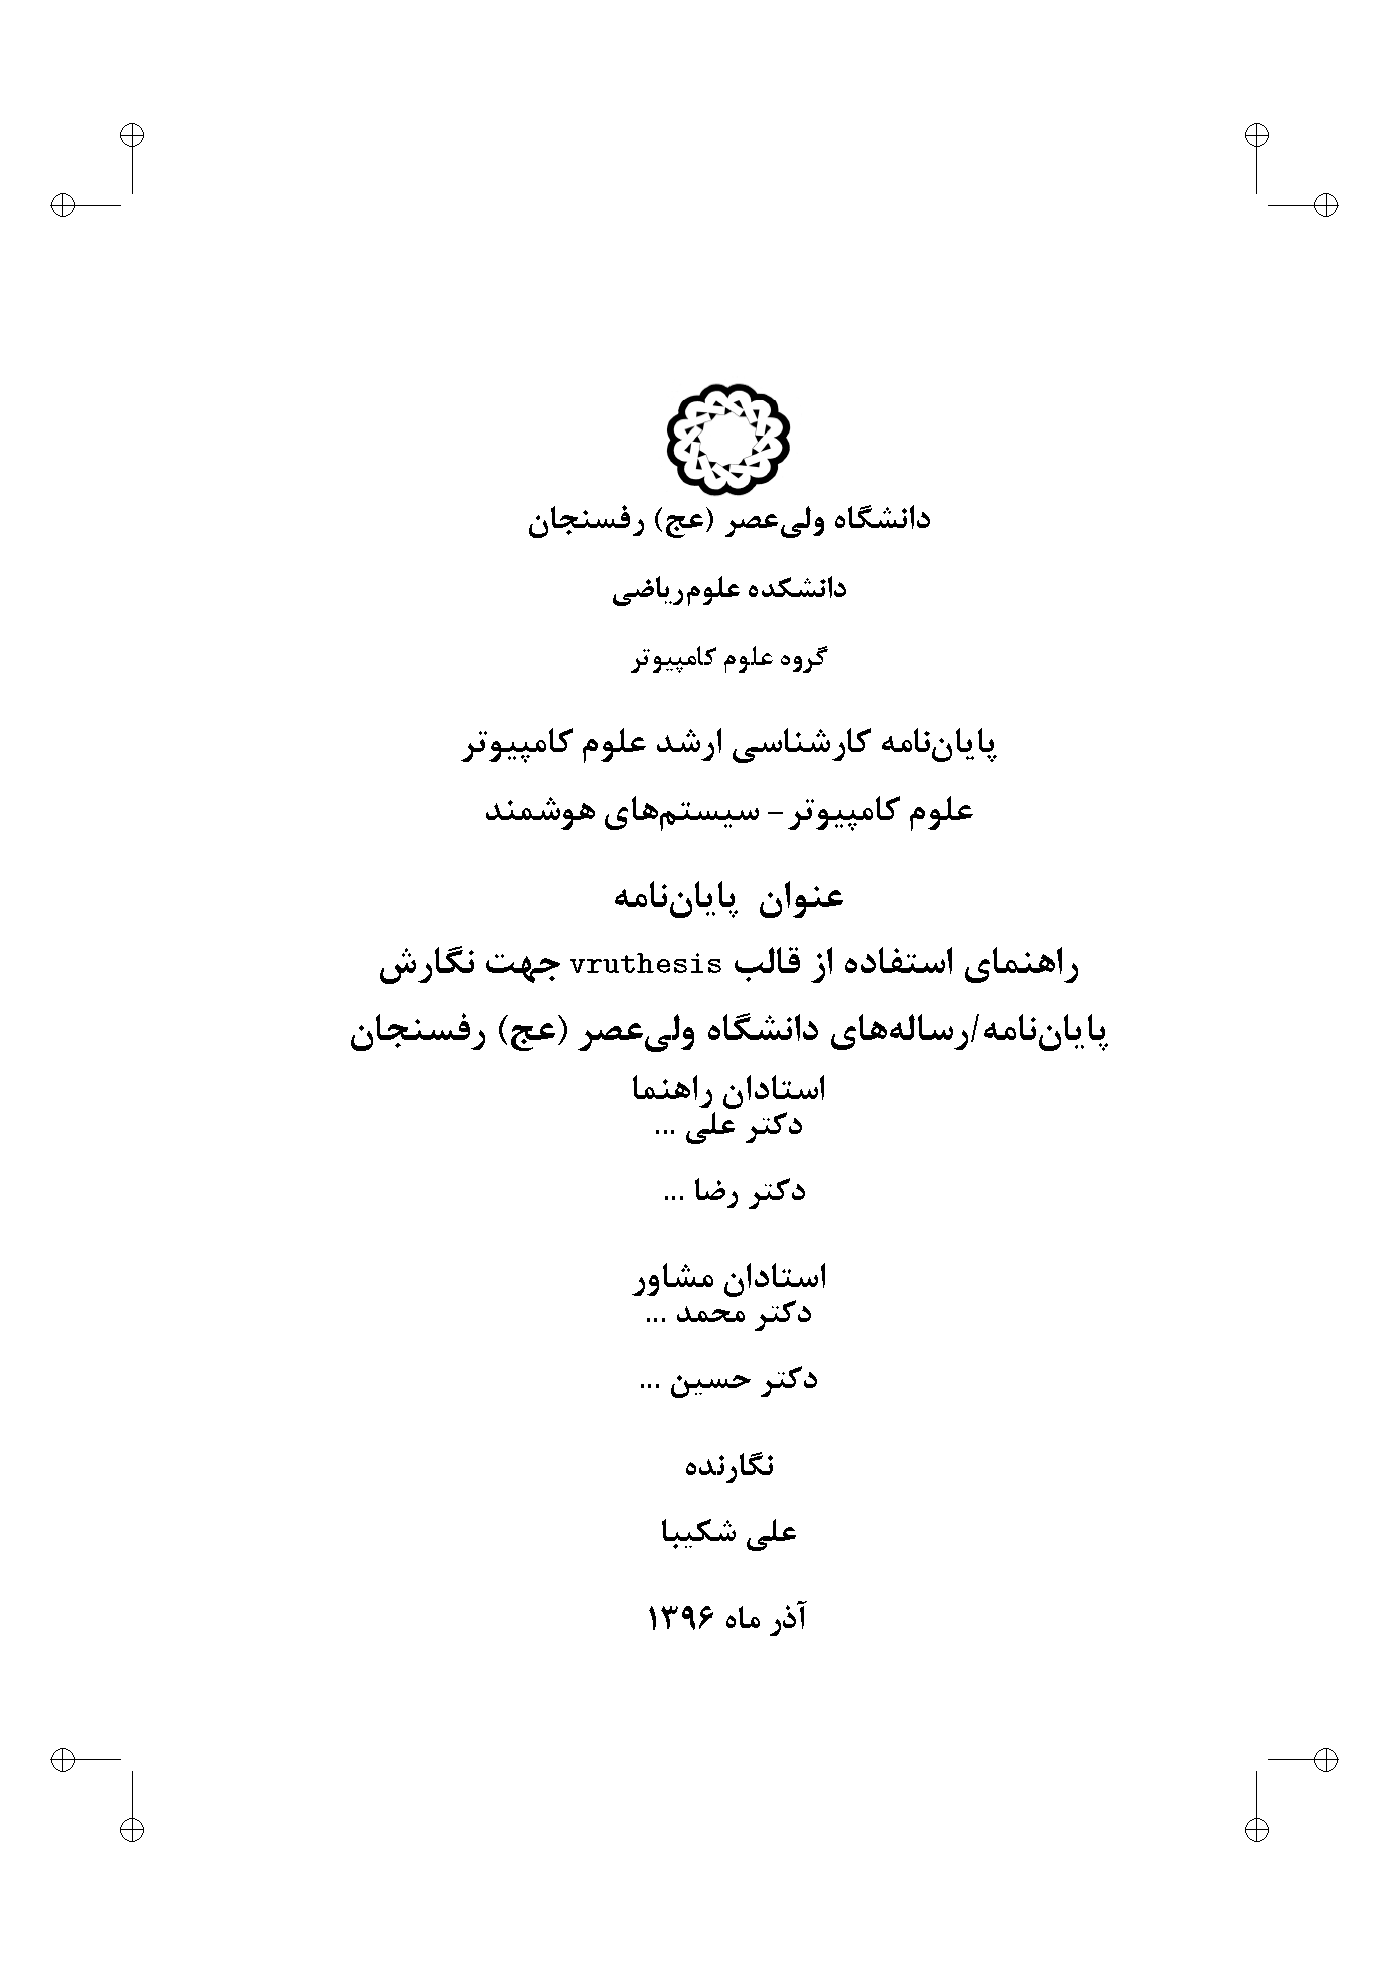
\includegraphics[width=\textwidth]{a.png}
		\caption{نمونه‌ی صفحه‌ی اول پایان‌نامه‌ی کارشناسی ارشد.}
		\label{app1}
	\end{figure}

	\begin{figure}
		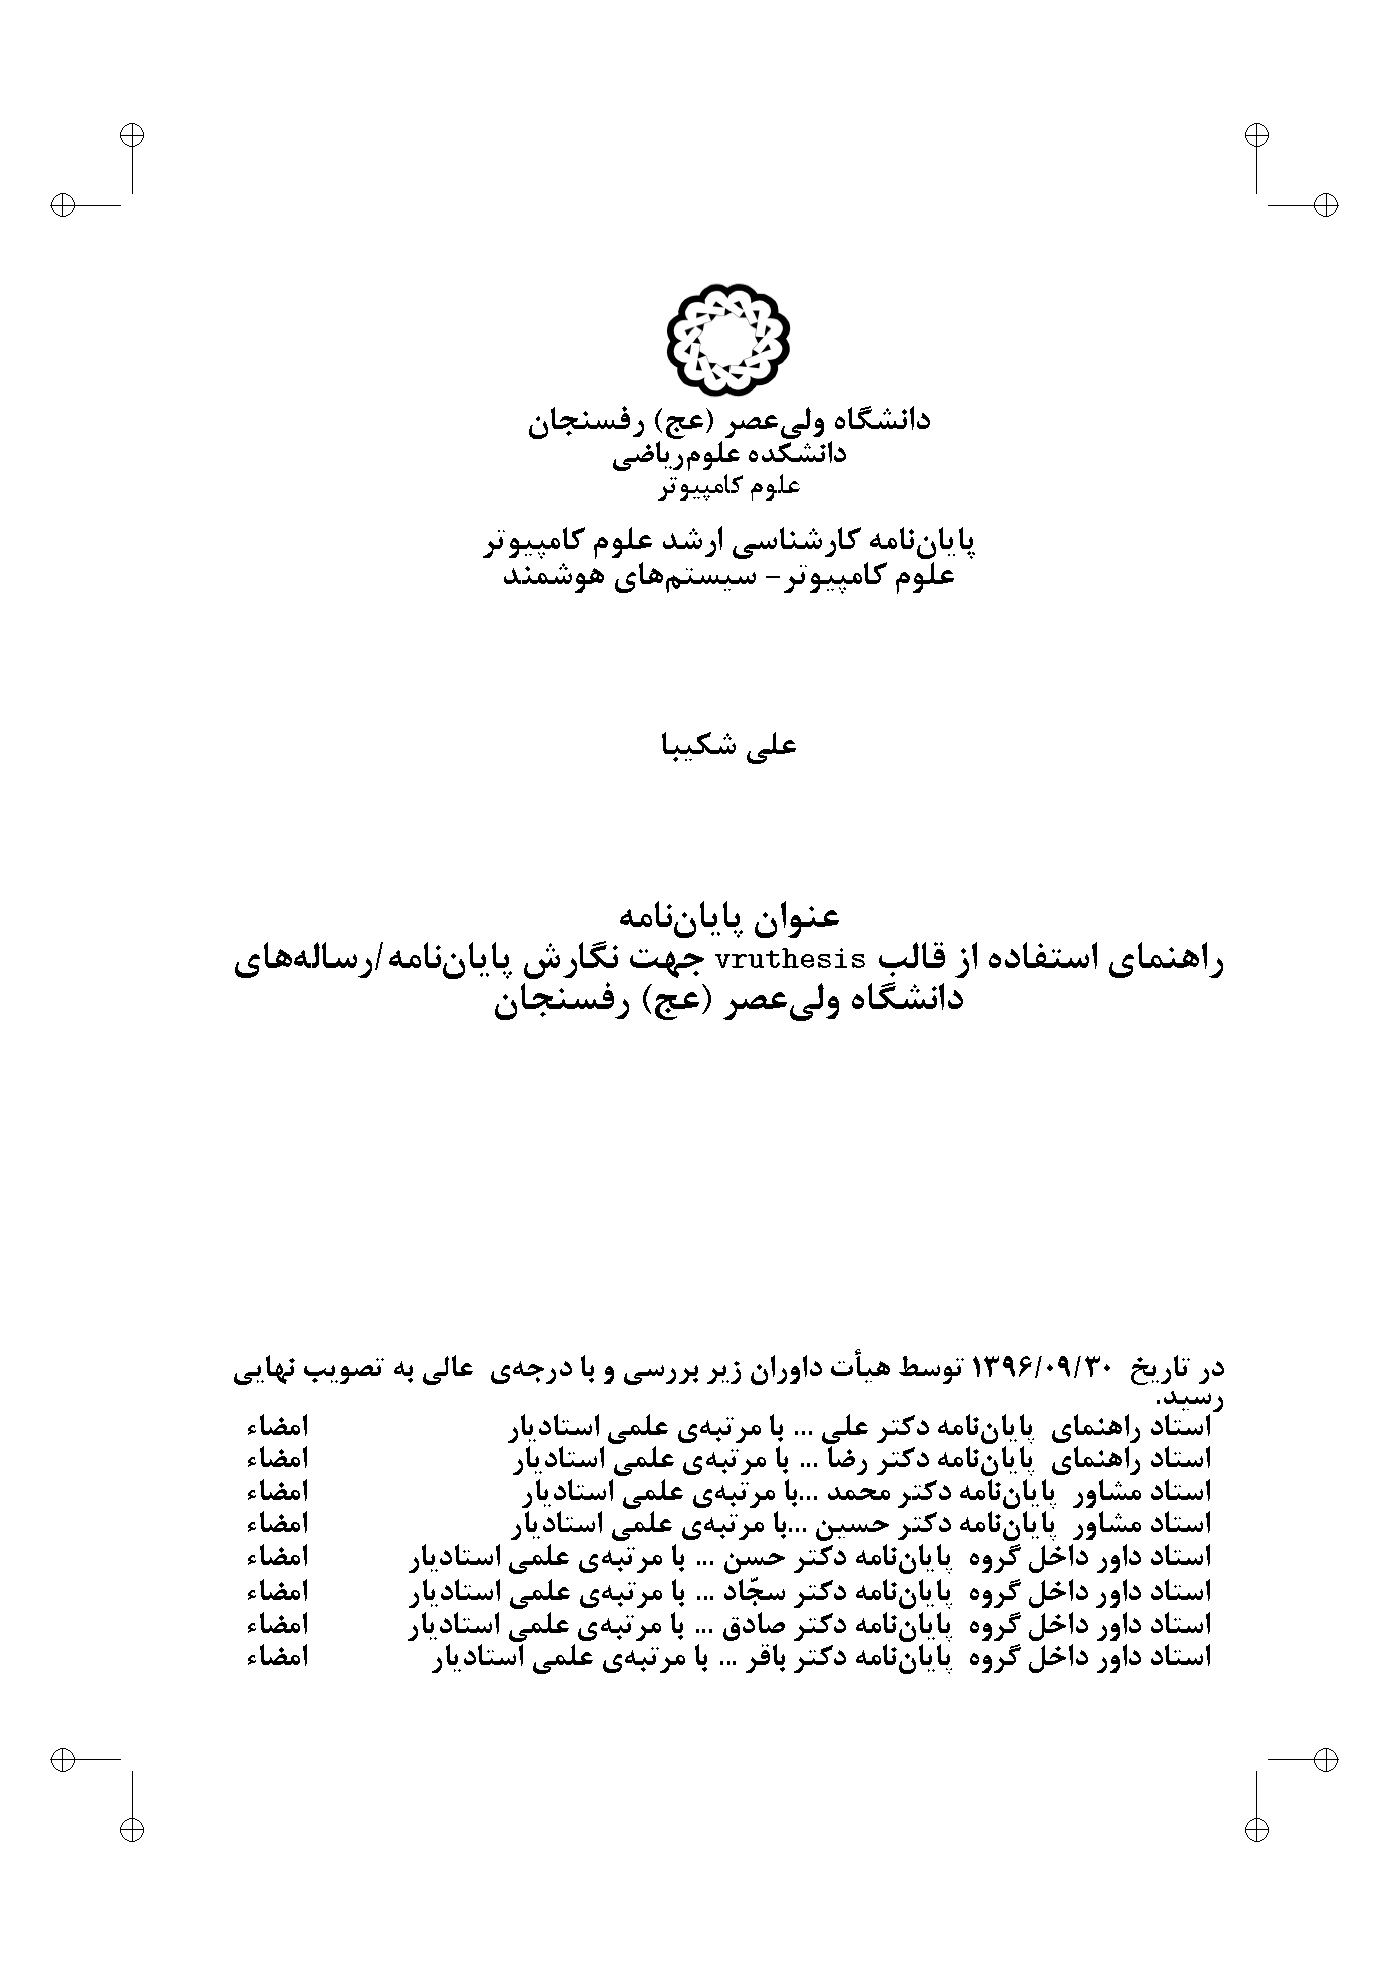
\includegraphics[width=\textwidth]{b.png}
		\caption{نمونه‌ی تصویب‌نامه‌ی پایان‌نامه‌ی کارشناسی ارشد.}
		\label{app2}
	\end{figure}

	\begin{figure}
		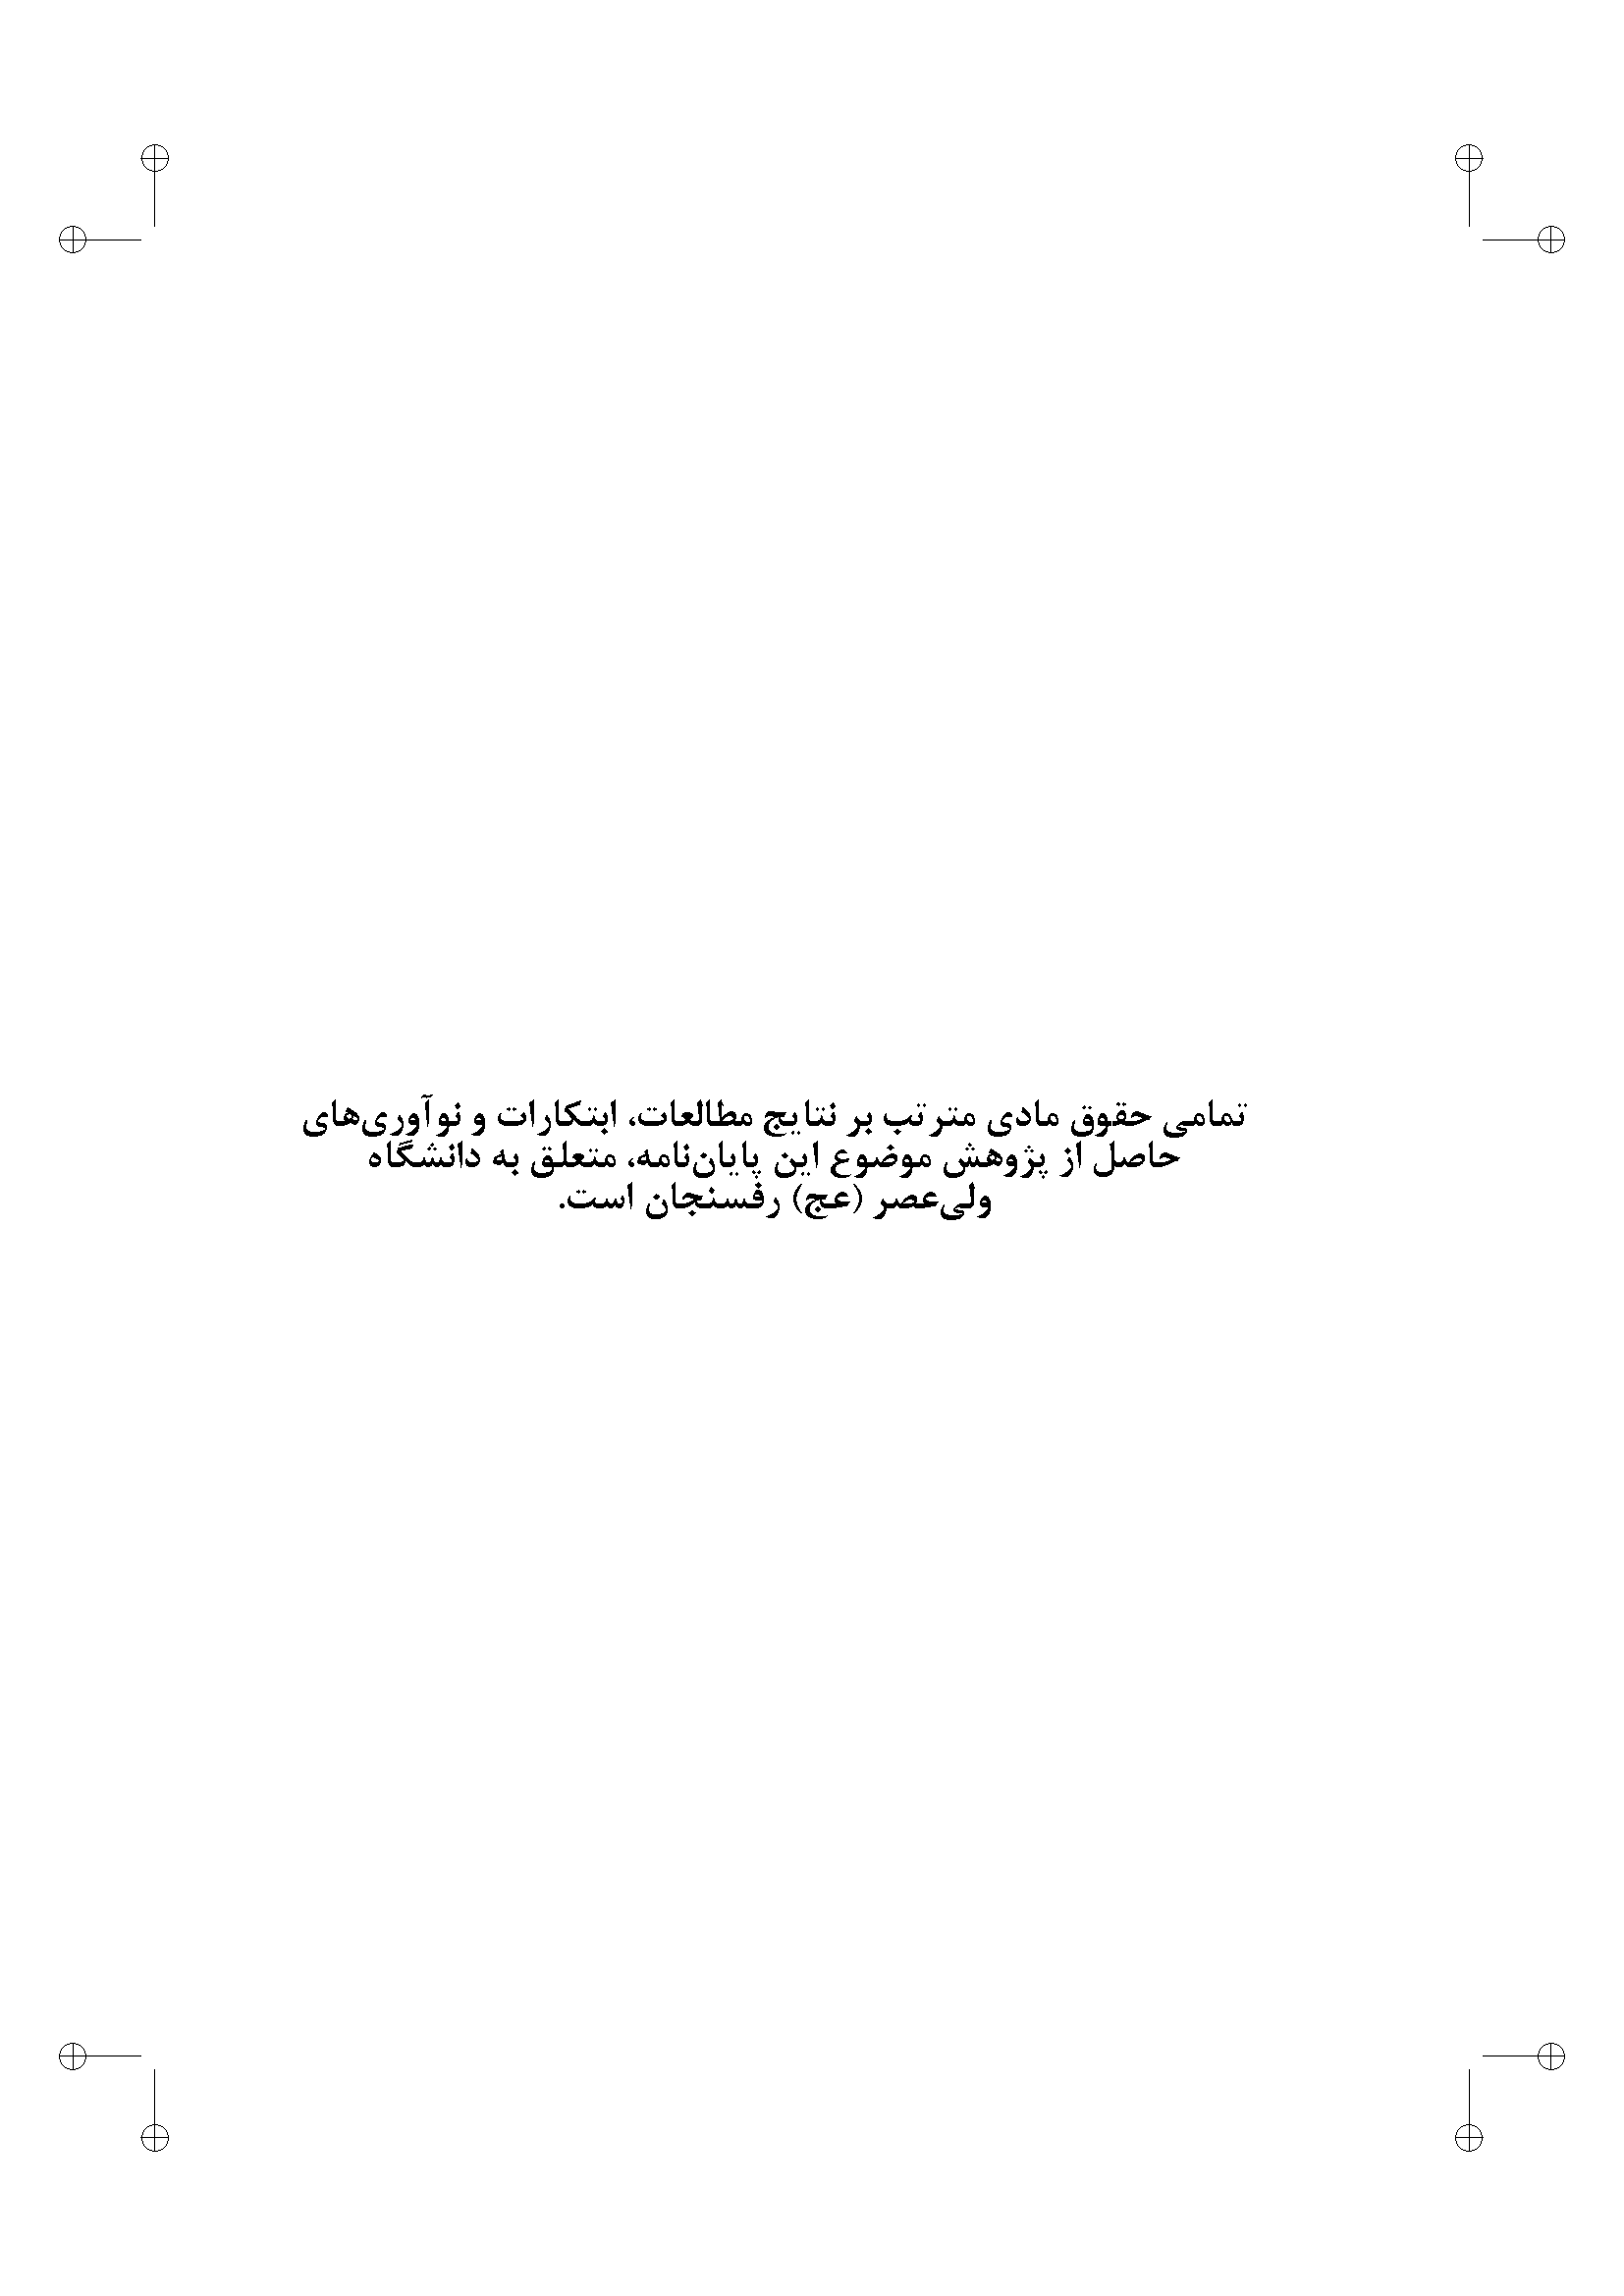
\includegraphics[width=\textwidth]{d.png}
		\caption{تعهدات حقوقی.}
		\label{app4}
	\end{figure}

	\begin{figure}
		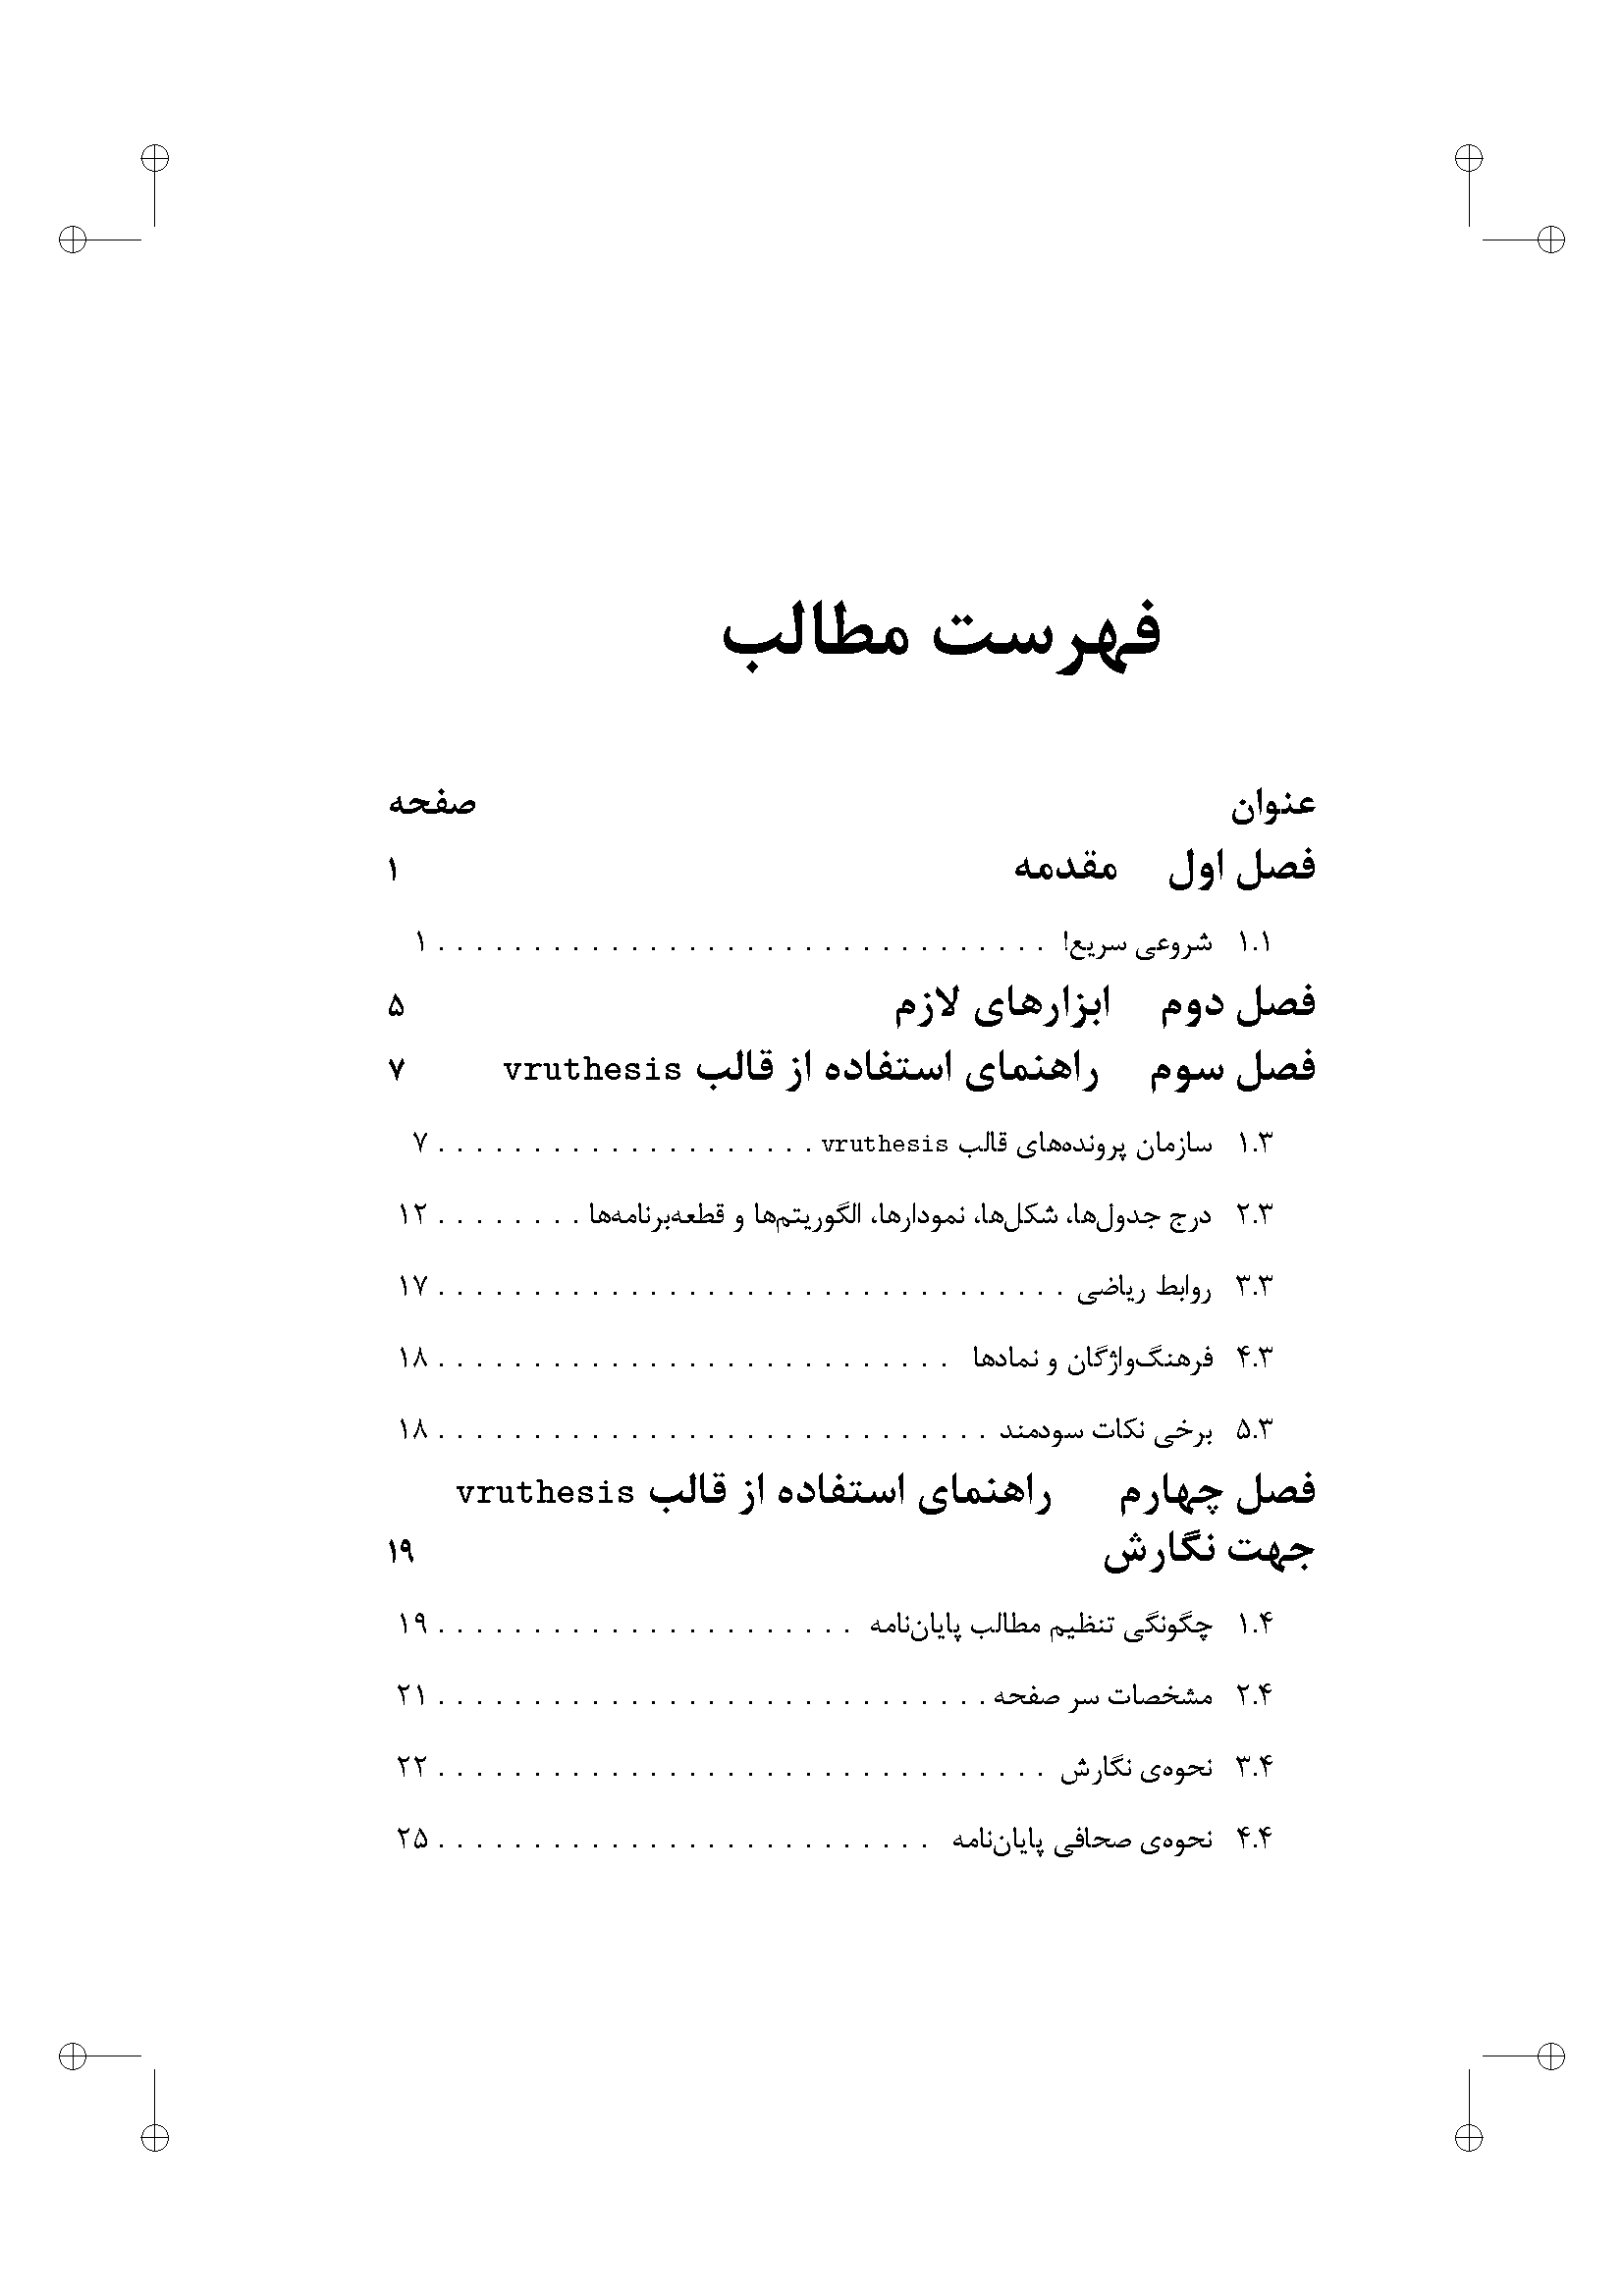
\includegraphics[width=\textwidth]{e.png}
		\caption{نمونه‌ای از فهرست مطالب.}
		\label{app5}
	\end{figure}

	\begin{figure}
		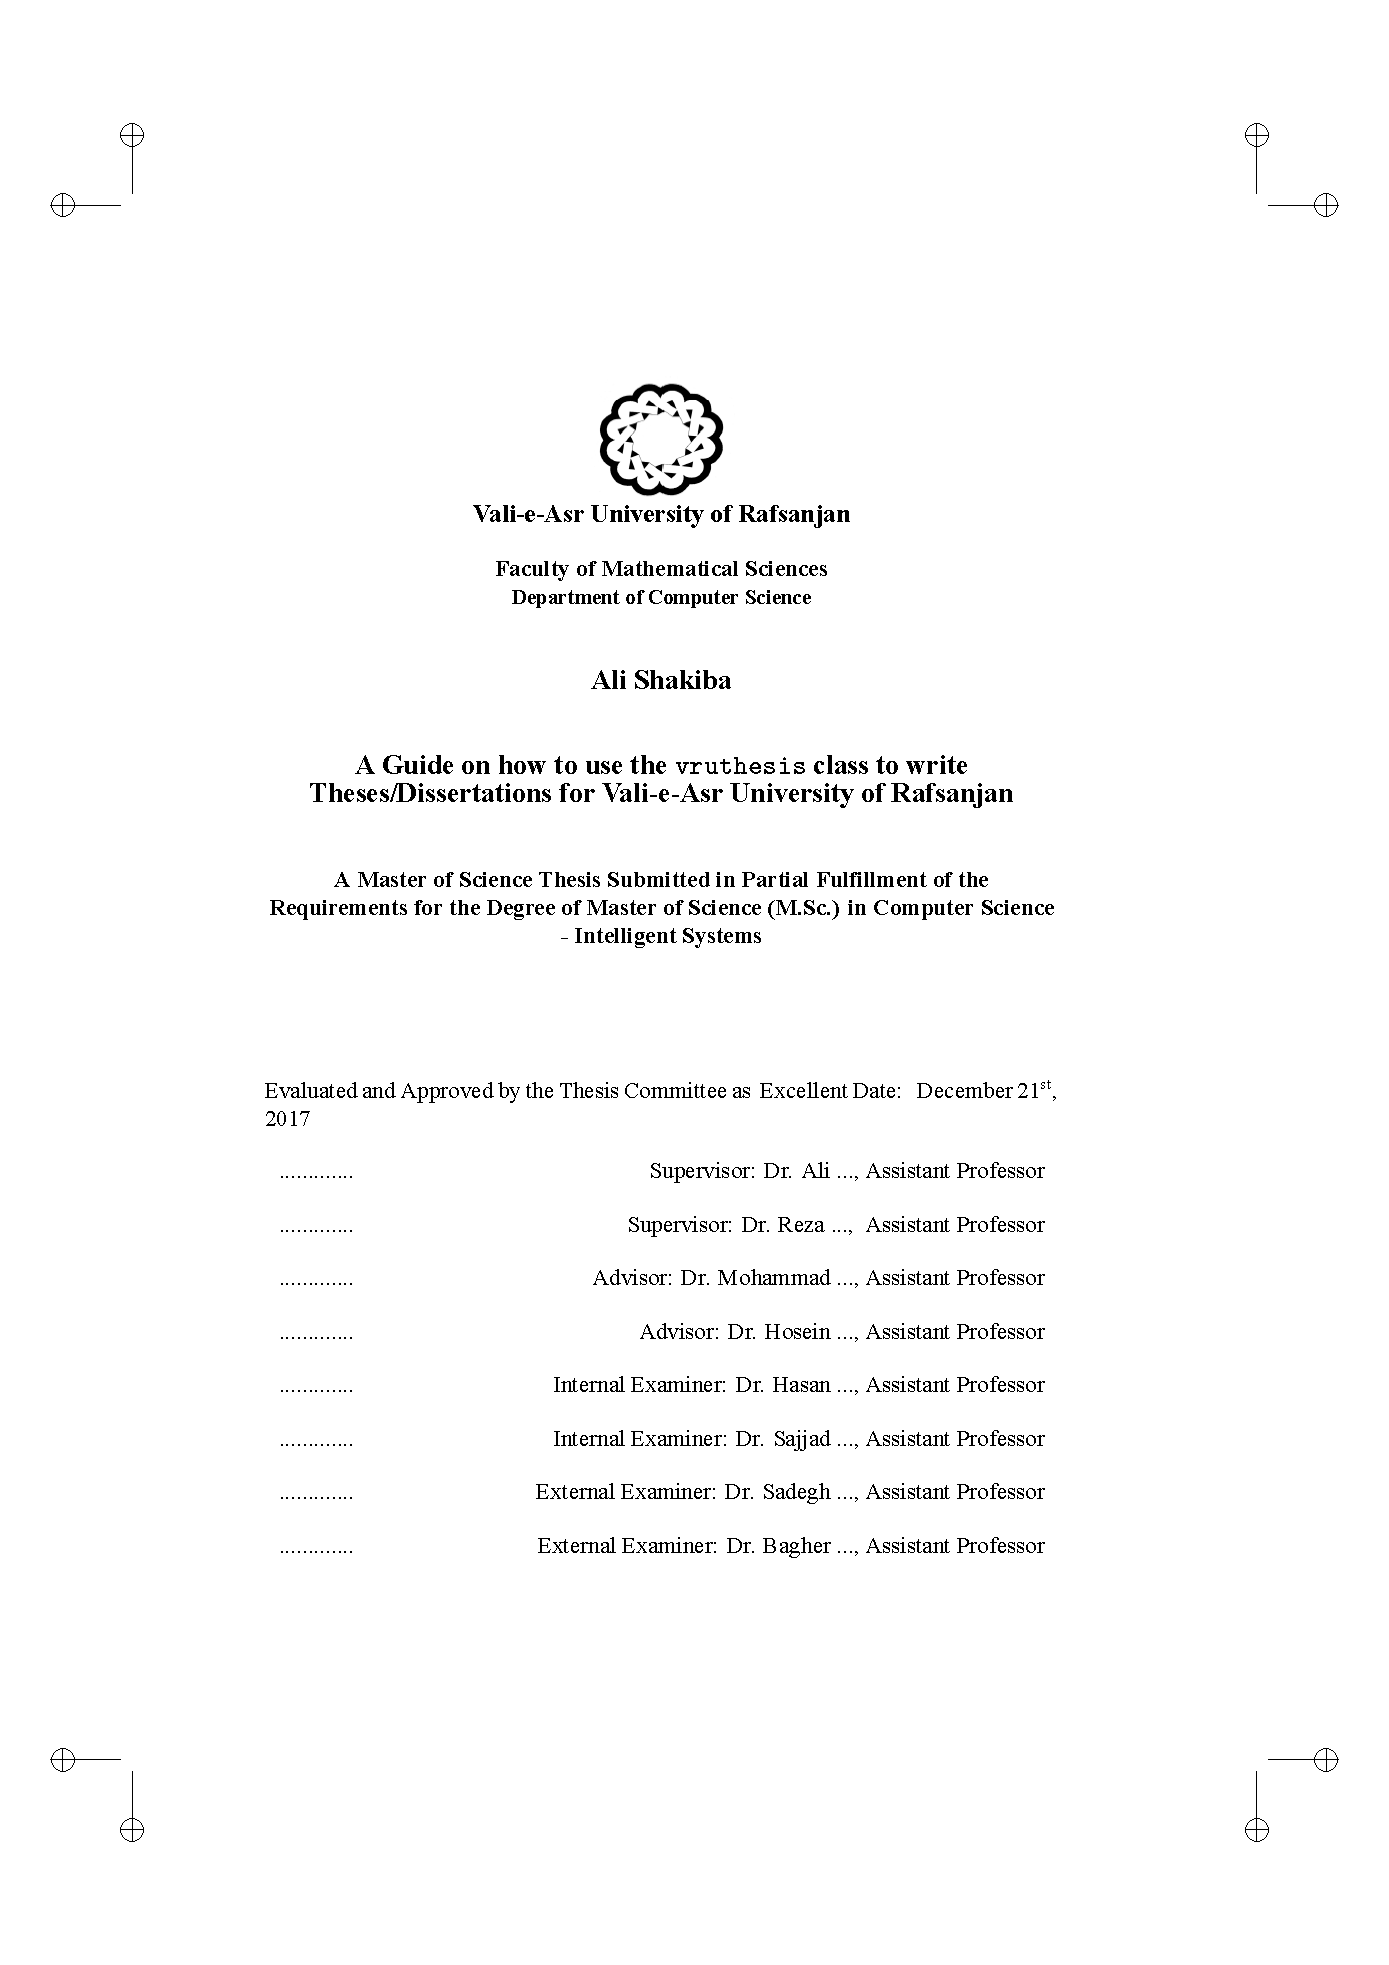
\includegraphics[width=\textwidth]{c.png}
		\caption{نمونه‌ی تصویب‌نامه‌ی پایان‌نامه‌ی کارشناسی ارشد به زبان انگلیسی.}
		\label{app3}
	\end{figure}

	\begin{figure}
		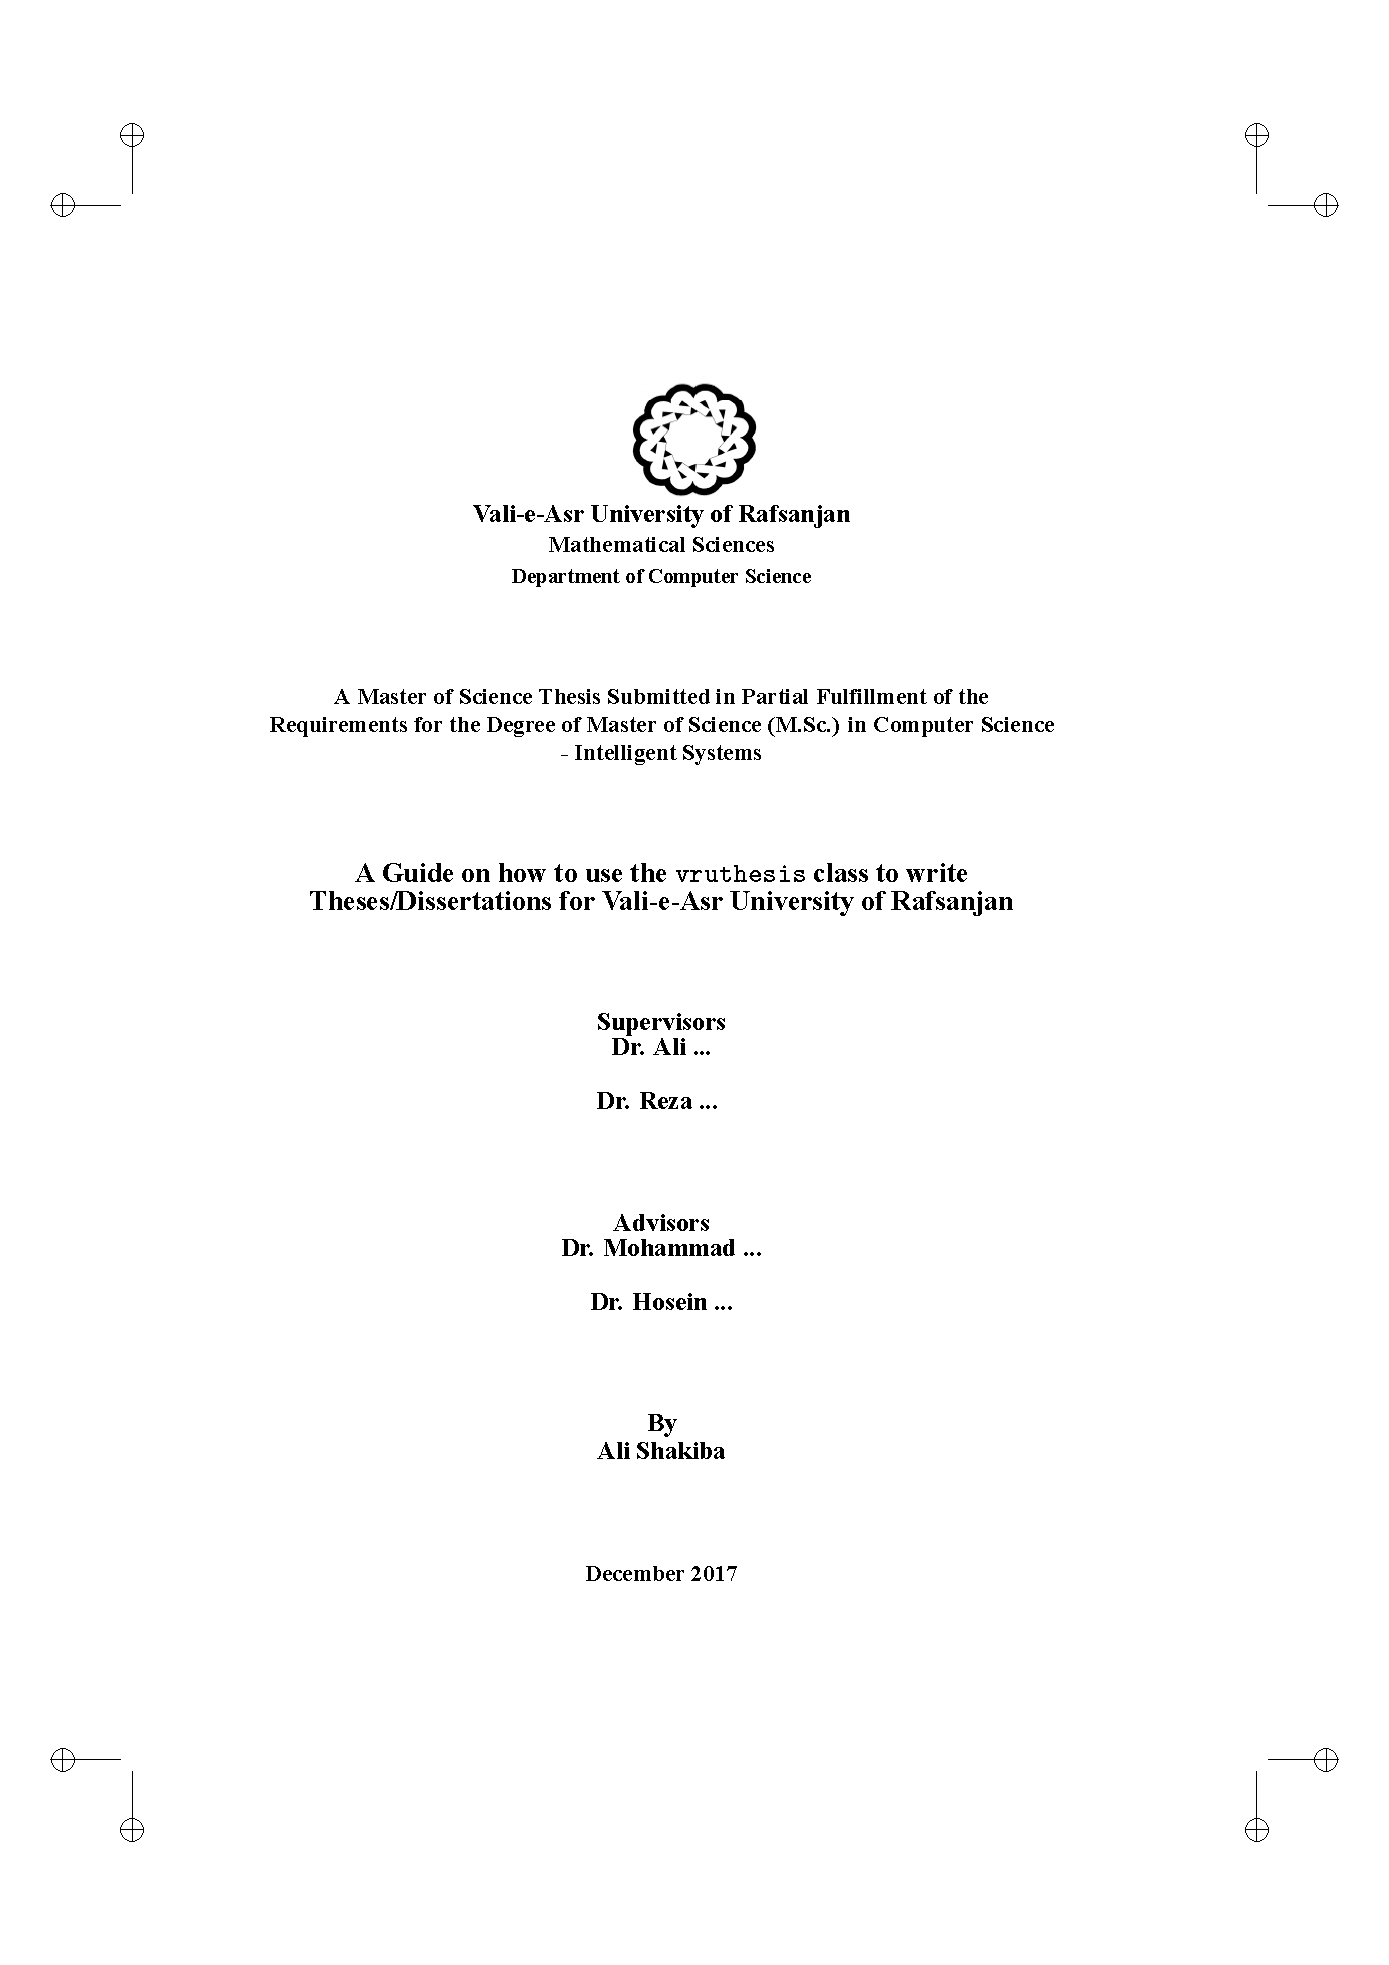
\includegraphics[width=\textwidth]{f.png}
		\caption{نمونه‌ی صفحه‌ی آخر پایان‌نامه‌ی کارشناسی ارشد.}
		\label{app6}
	\end{figure}

% +rl|از این قسمت به بعد را به هیچ وجه تغییر ندهید.$
	% لطفا هیچ تغییری در این فایل صورت ندهید.
	\cleardoublepage
	\printglossary
	\cleardoublepage
	\cleardoublepage
	\addcontentsline{toc}{chapter}{فهرست مراجع}
	\bibliography{references}
	\vrutitleen
\end{document}
		\end{mynewverbatim}
		\caption{محتویات \gls*{file} \lr{\texttt{thesis.tex}} نمونه.}
		\label{fig:ch1:thesis}
	\end{figure}
	این \gls{file} برای \gls{typeset} پایان‌نامه‌های کارشناسی ارشد دانشکده‌ی ریاضی در قطع وزیری، با چاپ دورو آماده شده است. همچنین، به منظور سهولت در فرایند صحافی، خطوط راهنما جهت برش کاغذ، در هر صفحه نمایش داده شده اند. 
	
		قواعد زیر؛ تنها قواعدی هستند که برای \gls{typeset} پایان‌نامه‌ی خود، نیاز است تا بدانید:
	\begin{itemize}
		\item اطلاعات مورد نیاز برای تولید صفحات ابتدایی و انتهایی پایان‌نامه، مانند چکیده‌، تقدیم‌به و مانند آن، در \gls{file} \lr{\texttt{data.tex}} قرار دارند. 
		\item مطالب هر یک از فصل‌ها را در یکی از \glspl{file}ی \lr{\texttt{chapterX.tex}} قرار دهید.
		\item پیوست‌ها در  \glspl{file}ی \lr{\texttt{appendixX.tex}} قرار می‌گیرند.
		\item قالب تولید فهرست مراجع در خط $10$ تعیین می‌گردد. برای تولید موفقیت آمیز فهرست مراجع، وجود \gls{file} \lr{\texttt{BibStyle.bst}} که \lr{\texttt{BibStyle}} بیانگر قالب مورد استفاده است؛ الزامی است.
		\item اطلاعات مربوط به مراجع در \gls{file} \lr{\texttt{references.bib}} به صورت \lr{bibtex} قرار می‌گیرند.
		\item واژگان در \gls{file} \lr{\texttt{gloss.tex}} و اختصارات و نمادها در \gls{file} \lr{\texttt{acronym.tex}} تعریف می‌شوند.
		\item دستورات لازم برای تولید خروجی در شکل \ref{fig:ch1:output_cmd} آمده‌اند. 
		\item وجود \glspl{file}ی \lr{\texttt{vruthesis.cls}}، \lr{\texttt{settings.tex}}، \lr{\texttt{data.tex}}، و \lr{\texttt{finalpart.tex}} جهت تولید خروجی موفق، الزامی است.
		\item در صورت نیاز برای \gls{typeset} رساله‌ی دکتری، در خط اول \gls{file} \lr{\texttt{chapterX.tex}}، کلمه‌ی \lr{phd} را به ویژگی‌ها اضافه نمایید.
		\item در صورتی که پایان‌نامه‌ی شما فاقد الگوریتم است؛ فهرست الگوریتم‌ها را با برداشتن کلمه‌ی \lr{alg} از ویژگی‌های خط اول \gls{file} \lr{\texttt{chapterX.tex}}، غیر فعال نمایید.
	\end{itemize}
				\begin{figure}
		\begin{latin}
\centering
	\begin{verbatim}
	xelatex -synctex=-1 thesis.tex
bibtex8 -W -c cp1256fa thesis
xindy -L persian-variant1 -C utf8 -I xindy -M thesis.xdy 
        -t thesis.glg -o thesis.gls thesis.glo
xindy -L persian-variant1 -C utf8 -I xindy -M thesis.xdy 
        -t thesis.blg -o thesis.bls thesis.blo
xindy -L english -C utf8 -I xindy -M thesis.xdy -t thesis.alg 
        -o thesis.acr thesis.acn
xelatex -synctex=-1 thesis.tex
xelatex -synctex=-1 thesis.tex
	\end{verbatim}
	\end{latin}
\caption{دستورات لازم برای تولید خروجی نهایی به قالب \gls*{pdf}.}
\label{fig:ch1:output_cmd}
\end{figure}
\section{یک بخش آزمایشی}
در این قسمت، نمونه‌ای از بخش‌بندی‌های ممکن نمایش داده می‌شوند.
	\subsection{یک زیربخش}
	زیربخش‌ها می‌توانند در صورت لزوم دارای زیرزیربخش باشند.
		\subsubsection{یک زیرزیربخش}
		لطفا توجه داشته باشید که بخش‌بندی بیش از چهار سطح، مجاز نیست.
\newpage
این متن جهت آزمودن تعداد خطوط در هر صفحه از ویکی‌پدیای فارسی درباره‌ی خوارزمی برداشته شده است. 
محمد بن موسی خوارزمی (زاده حدود سال ۷۸۰ میلادی و درگذشته ۸۵۰ میلادی) ریاضیدان، ستاره‌شناس، فیلسوف، جغرافیدان و مورخ شهیر ایرانی[۲] در دوره عباسیان است. وی در حدود سال ۷۸۰ میلادی (قبل از ۱۸۵ قمری)[۱] در خوارزم زاده شد. ابن ندیم و قفطی اصالت او را از خوارزم می‌دانند. لقب وی معمولاً اشاره به شهر خوارزم دارد که همان خیوه کنونی واقع در جنوب دریاچه آرال مرکزی و بخشی از جمهوری ازبکستان کنونی است.[۱] شهرت علمی وی مربوط به کارهایی است که در ریاضیات، به‌ویژه در رشته جبر، انجام داده به‌طوری‌که هیچ‌یک از ریاضیدانان سده‌های میانه مانند وی در فکر ریاضی تأثیر نداشته‌اند و وی را «پدر جبر» نامیده‌اند.[۳] جرج سارتن، مورخ مشهور علم، در طبقه‌بندی سده‌ای کتاب خود مقدمه‌ای بر تاریخ علم سده نهم میلادی را «عصر خوارزمی» می‌نامد.[۴][۵]

خوارزمی ریاضی‌دان بنام قرون وسطی است که حاصل تحقیقات و تألیفات او هنوز مورد استفاده می‌باشد و کتاب جبر و مقابله او را بسیاری از مترجمان مشهور قرون وسطی ترجمه کرده‌اند. بیشترین چیره‌دستی وی در حل معادله‌های خطی و درجه دوم بوده‌است. کتاب Algoritmi de numero Indorum که ترجمه کتاب جمع و تفریق با عددهای هندی او به لاتین است باعث شد تا دستگاه عددی در اروپا از عددنویسی رومی به عددنویسی هندی-عربی تغییر یابد؛ چیزی که هنوز نیز در اروپا و دیگر نقاط جهان فراگیر است.[۶] واژه جبر را اروپائیان بطور کلی از کتاب خوارزمی و اصطلاح امروزی الگوریتم (Algorithmus) از نام خوارزمی گرفته شده‌است. به هنگام خلافت مأمون، وی عضو دارالحکمه که مجمعی از دانشمندان در بغداد به سرپرستی مأمون بود، گردید. خوارزمی کارهای دیوفانت را در رشته جبر دنبال کرد و به بسط آن پرداخت.
گویند قبل از اینکه محمد بن موسی خوارزمی در دارالحکمه مستقر شود او را به سرزمین هند فرستادند تا حساب هندی را بیاموزد خوارزمی پس از بازگشت از هند دو اثر «حساب الهند» و دیگری «الجبر و المقابله» را نگاشت. وی نتایجی را که یونانیان و هندیان بدست آورده بودند را تلفیق کرد و بدین ترتیب سبب انتقال مجموعه‌ای از معلومات جبری حسابی شد که در ریاضیات قرون وسطی تأثیر عمیقی گذاشت.[۱۱]
محمد بن موسی خوارزمی در قرن سوم هجری، علمی را برای نخستین بار صورتبندی و تدوین کرد که خود آن را «الجبر و المقابله» نامید، علمی که تمام شرایط یک دانش واقعی را داشت، یعنی همان که اروپاییان از آن به «ساینس» تعبیر می‌کنند. این ریاضی‌دان توانست با این دانش تمام معادلات درجه دوم زمان خود راحل و راه را برای حل معادلات درجه بالاتر هموار کند.
ر اساس الواح بابلی و آثار برجای‌مانده از محاسبه‌گران هندی در عهد باستان، مردمان بابل و هند به حل حالات خاصی از معادلات درجه دوم موفق شده بودند، اما آن‌ها راه حل‌های خود را فقط به صورت دستور ارائه کردند؛ یعنی این راه حل‌ها، که برای رفع نیازهای زندگی روزمره آنان ارائه شده بودند و نه به منظور گسترش دانش ریاضی، فاقد براهین علمی بودند. ابتکار خوارزمی در آن است که وی نخست همه معادلات درجه دوم شناخته‌شده زمانش را بررسی می‌کند؛ در مرحله دوم روش حل هریک از آن‌ها را ارائه می‌دهد؛ سرانجام در مرحله سوم، این روش‌ها را با کمک علم هندسه اثبات می‌کند؛ مؤلفه‌هایی که درمجموع علم جدیدی به نام «جبر» را تشکیل می‌دهند. این علم، که از طریق ترجمه‌های لاتینی کتاب خوارزمی در قرون وسطی به اروپا راه یافت، هم در قرون وسطی و هم در عصر رنسانس تحول بزرگی در علم ریاضیات را موجب شد، چنان‌که در قرن شانزدهم میلادی نیکولو تارتالیا[واژه‌نامه ۳] و کاردان،[واژه‌نامه ۴] ریاضی‌دانان ایتالیایی که با ترجمه لاتینی جبر و مقابله، آشنا بودند روش این ریاضی‌دان ایرانی را برای حل معادله درجه سوم تعمیم دادند و بدین‌ترتیب گام دیگری در گسترش ریاضیات برداشتند.[۱۳]
خوارزمی کارهای دیوفانتوس[واژه‌نامه ۵] را در رشته جبر را دنبال کرد و به بسط آن پرداخت با توجه به این ابداع بزرگ ثابت کردند که علم نژاد و فرهنگ نمی‌شناسد و محصول ذهن انسان‌های متفکری است که در این عرصه تلاش می‌کنند.[۱۳] این علم از طریق کتاب وی «المختصر فی حساب الجبر و المقابله» در جهان اسلام شهرت یافت و ریاضیدانان بعد از خود را بشدت تحت تأثیر قرار داد که در سده ۱۲ میلادی به لاتین ترجمه شد.[۱۴]
	\chapter{ابزارهای لازم}
	برای تولید یک خروجی مناسب، نیاز به نصب و استفاده از ابزارهای زیر دارید:
	\begin{itemize}
		\item یک توزیع \lr{\LaTeX} مانند \lr{TeXLive}، \lr{MiKTeX} یا \lr{MaxTeX}. لازم به ذکر است که این قالب با استفاده از توزیع \lr{TeXLive 2017} تولید شده‌است.
		\item یک ویرایشگر متن مانند \lr{bidiTeXMaker}، \lr{TeXStudio}، \lr{TeXWorks}، \lr{Notepad++} و مانند آن‌ها. در این مورد، پیشنهاد می‌شود تا از \lr{bidiTeXMaker} یا \lr{TeXWorks} استفاده کنید.
	\end{itemize}

برای \gls{download} \gls{file} \lr{TeXLive 2017}، می‌توانید از آدرس \url{https://www.tug.org/texlive/acquire-iso.html} استفاده نمایید. در صورتی که در شبکه‌ی داخلی دانشگاه حضور دارید؛ توصیه می‌شود تا از آدرس \url{ftp://ftp.vru.ac.ir/Professor/Technical/A.shakiba/} استفاده کنید. لازم به ذکر است که \gls{file} حجیم و در حدود $4$ گیگابایت است. این راهنما بر مبنای راهنمای موجود در سایت پارسی‌لاتک\LTRfootnote{\url{http://www.parsilatex.com/wiki/\rl{راهنمای_نصب_تک‌لایو}}} نوشته شده‌ است.

به منظور یادگیری \gls{typeset} با \lr{\LaTeX} توصیه می‌شود تا از کتاب «مقدمه‌ای نه چندان کوتاه بر \lr{\LaTeX}»، ترجمه‌ی آقای مهدی امیدعلی\LTRfootnote{\url{https://www.ctan.org/tex-archive/info/lshort/persian}} استفاده نمایید. همچنین، می‌توانید در کارگاه‌های آموزشی دانشکده‌ی علوم ریاضی در ابتدای هر ترم، شرکت کنید.

\begin{figure}
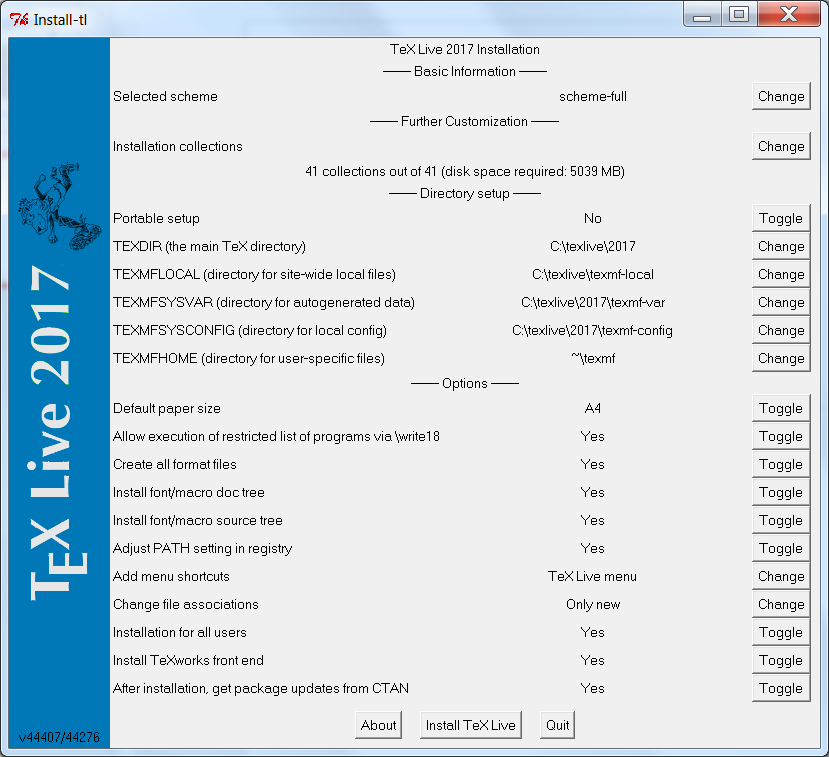
\includegraphics[width=.7\textwidth]{figs/texlive2017.png} 
\caption{پنجره‌ی نصب \lr{TeXLive 2017}.}
\end{figure}
	\chapter{راهنمای استفاده از قالب \texttt{vruthesis}}

برای \gls{typeset} پایان‌نامه‌ها و رساله‌های دانشکده‌ی علوم ریاضی، می‌توان از قالب \texttt{vruthesis} استفاده نمود. در این فصل، ابتدا در بخش \ref{sec:file_org} به سازمان \glspl{file}ی مورد استفاده در این قالب پرداخته می‌شود. شیوه‌ی قرارگیری جدول‌ها، شکل‌ها، نمودارها، الگوریتم‌ها و قطعه‌برنامه‌ها در بخش \ref{sec:figs_tbls_algs_codes} ذکر می‌شود. بخش \ref{sec:eqs} به \gls{typeset}ِ روابط ریاضی اختصاص دارد. نکات مربوط به فرهنگ‌واژگان و نمادها در بخش \ref{sec:gloss} ذکر شده‌اند. در پایان، بخش \ref{sec:faq}، برخی از نکات سودمند در استفاده از این قالب را گوشزد می‌کند.

\section{سازمان \glspl*{file}ی قالب \texttt{vruthesis}}\label{sec:file_org} 
	متن یک پایان‌نامه به طور معمول، یک متن طولانی است. بنابراین، بهتر است تنظیمات \gls{formatting} و محتوای پایان‌نامه را از یکدیگر جدا کنیم. تنظیمات \gls{formatting} در \gls{file} \texttt{vruthesis.cls} آمده است. علاوه بر این، به منظور مدیریت بهتر بر محتوا، محتوای پایان‌نامه نیز بر اساس فصل در \glspl{file}ی متعدد، تقسیم‌بندی شده‌اند. به منظور سادگی بیشتر، نمونه‌ی یک پایان‌نامه‌ی کارشناسی ارشد و نمونه‌ی یک رساله‌ی دکتر در \gls{site} دانشکده قرار گرفته‌اند. هر یک از این نمونه‌ها، شامل چند \gls{file} مختلف هستند. فهرست این \glspl{file} و کاربرد هر یک از آن‌ها در جدول \ref{tbl:fileList} آمده است. استفاده از دستوراتی که در شرح آن‌ها، عبارت «در صورت وجود» آمده است؛ اختیاری است و در صورتی که این دستورات در \gls{file} \verb|data.tex| نیامده باشند یا به صورت توضیح درج شده باشند؛ خروجی به صورت متناسب تولید می‌گردد.

\begin{table}[ht]
	\caption[\glspl*{file}ی موجود در نمونه‌ی پایان‌نامه دانشکده.]{فهرست و کاربرد \glspl*{file}ی موجود در نمونه‌ی پایان‌نامه‌ی دانشکده‌ی علوم ریاضی.}
	\label{tbl:fileList}
	\centering
	\begin{tabular}{| R{0.60\textwidth} | L{0.25\textwidth} |}
		\hline 
		\textbf{شرح} & \textbf{نام \gls{file}} \\
		\hline
		\glspl{file} اصلی پایان‌نامه، شامل ارجاع به تنظیمات، محتوا و سایر دستورات & \texttt{thesis.tex} \\ \hline
		قالب \texttt{vruthesis} & \texttt{vruthesis.cls} \\ \hline
		اطلاعات مربوط به صفحات ابتدایی و انتهایی پایان‌نامه مانند عنوان (لاتین)، چکیده (لاتین) و مانند آن & \texttt{data.tex} \\ \hline
		تعریف منابع و مآخذ به صورت \texttt{bibtex} &  \texttt{references.bib} \\ \hline
		\gls{formatting} مراجع مطابق با استاندارد \lr{IEEE} با تغییرات مصوب گروه علوم‌کامپیوتر &  \texttt{ieeetr-fa-vru.bst} \\ \hline
		\gls{formatting} مراجع مطابق با استاندارد \lr{ACM} با در نظر گرفتن مراجع فارسی &  \texttt{acm-fa.bst} \\ \hline
		محتویات مربوط به فصل \lr{X} پایان‌نامه &  \texttt{chapterX.tex} \\ \hline
		محتویات مربوط به پیوست \lr{X} پایان‌نامه &  \texttt{appendixX.tex} \\ \hline
		اطلاعات مورد نیاز برای ساخت فهرست واژگان & \texttt{gloss.tex} \\ \hline
		فهرست اختصارات و نمادها & \texttt{acronym.tex} \\ \hline
	\end{tabular}
\end{table}

	برای تولید \gls{file} نهایی پایان‌نامه در قالب \gls{pdf}، لازم است تا از موتور \lr{TeX Live 2017} استفاده شود. دستورات مورد نیاز برای تولید خروجی، در شکل \ref{fig:output_cmd} ذکر شده‌اند. 
	
	\begin{figure}
		\begin{latin}
\centering
	\begin{verbatim}
	xelatex -synctex=-1 thesis.tex
bibtex8 -W -c cp1256fa thesis
xindy -L persian-variant1 -C utf8 -I xindy -M thesis.xdy 
        -t thesis.glg -o thesis.gls thesis.glo
xindy -L persian-variant1 -C utf8 -I xindy -M thesis.xdy 
        -t thesis.blg -o thesis.bls thesis.blo
xindy -L english -C utf8 -I xindy -M thesis.xdy -t thesis.alg 
        -o thesis.acr thesis.acn
xelatex -synctex=-1 thesis.tex
xelatex -synctex=-1 thesis.tex
	\end{verbatim}
	\end{latin}
\caption{دستورات لازم برای تولید خروجی نهایی به قالب \gls*{pdf}.}
\label{fig:output_cmd}
\end{figure}

در پایان‌نامه‌ی نمونه، $5$ فصل و یک پیوست درنظر گرفته شده است. در صورتی که در پایان‌نامه‌ی خود، به فصل‌های (پیوست‌های) بیشتری نیاز دارید؛ می‌توانید با تهیه‌ی یک رونوشت از \gls{file} \texttt{chapterX.tex} (\texttt{appendixX.tex}) و ذخیره‌ی آن به نام دلخواه، فصل (پیوست) جدیدی را ایجاد کنید. لازم به ذکر است که برای لحاظ شدن فصل جدید در خروجی، نیاز است تا در \gls{file} \texttt{thesis.tex}، دستور
\begin{latin}
	\begin{verbatim}
	\include{chapterX}
	\end{verbatim}
\end{latin}
را پس از {\verb|\chapter{نتیجه‌گیری}
در این فصل، نتیجه‌گیری پایان‌نامه‌ی خود را درج کنید.
			|} یا آخرین فصل اضافه شده، قرار دهید. به طور مشابه، برای لحاظ شدن پیوست جدید در خروجی، لازم است تا دستور \verb|\include{appendixX}| پس از \verb|\chapter{یک پیوست}
مطالب این پیوست بر اساس راهنمای نگارش پایان‌نامه‌های تحصیلات تکمیلی در \cite{vru_grad_rules} تهیه شده‌اند. 

	\begin{figure}
		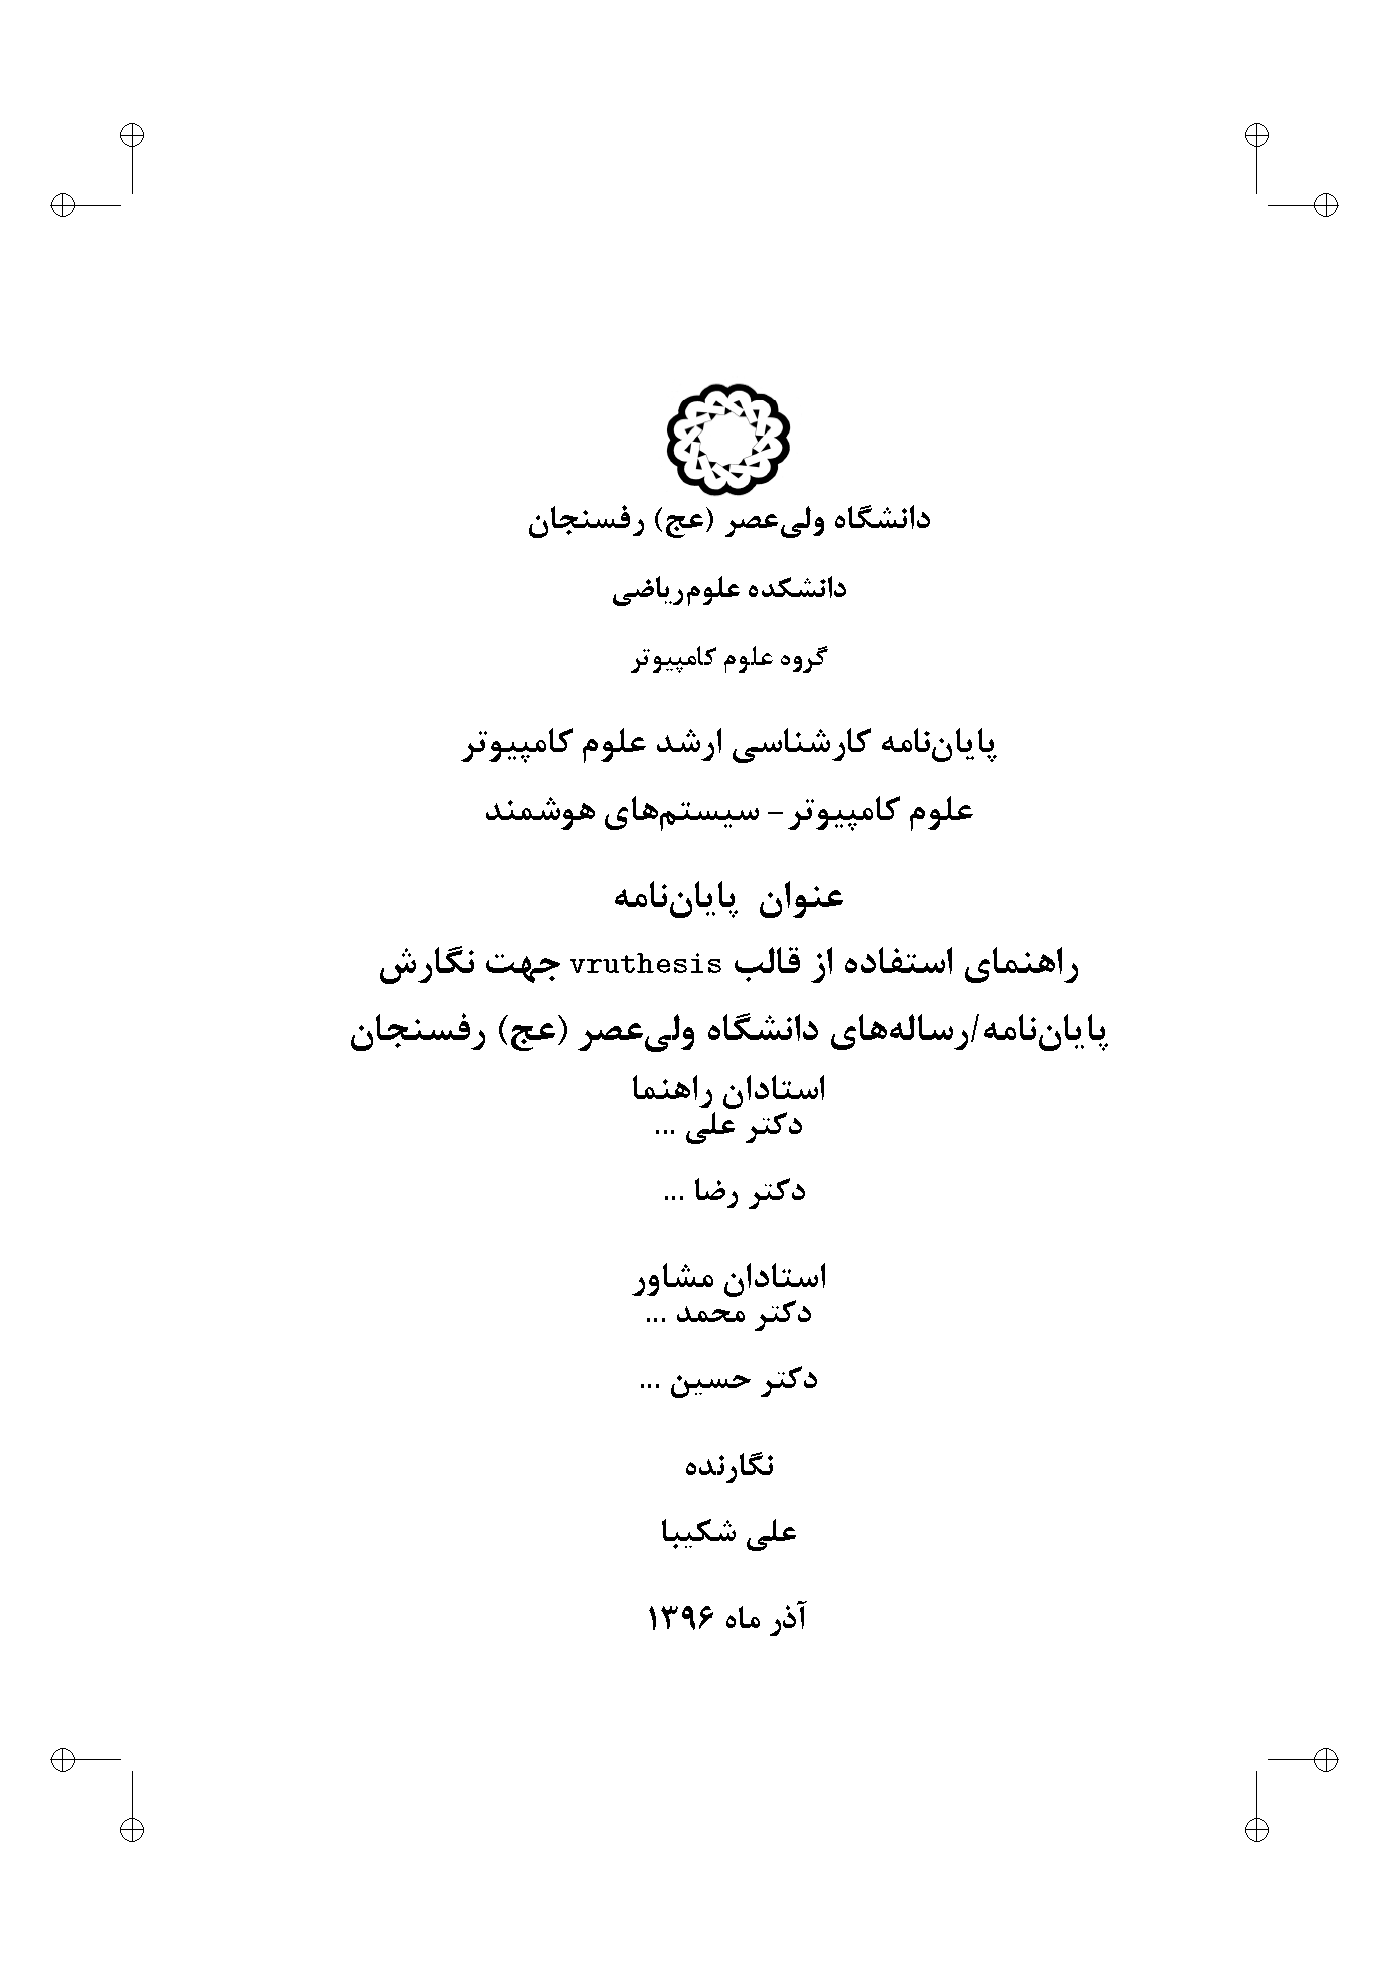
\includegraphics[width=\textwidth]{a.png}
		\caption{نمونه‌ی صفحه‌ی اول پایان‌نامه‌ی کارشناسی ارشد.}
		\label{app1}
	\end{figure}

	\begin{figure}
		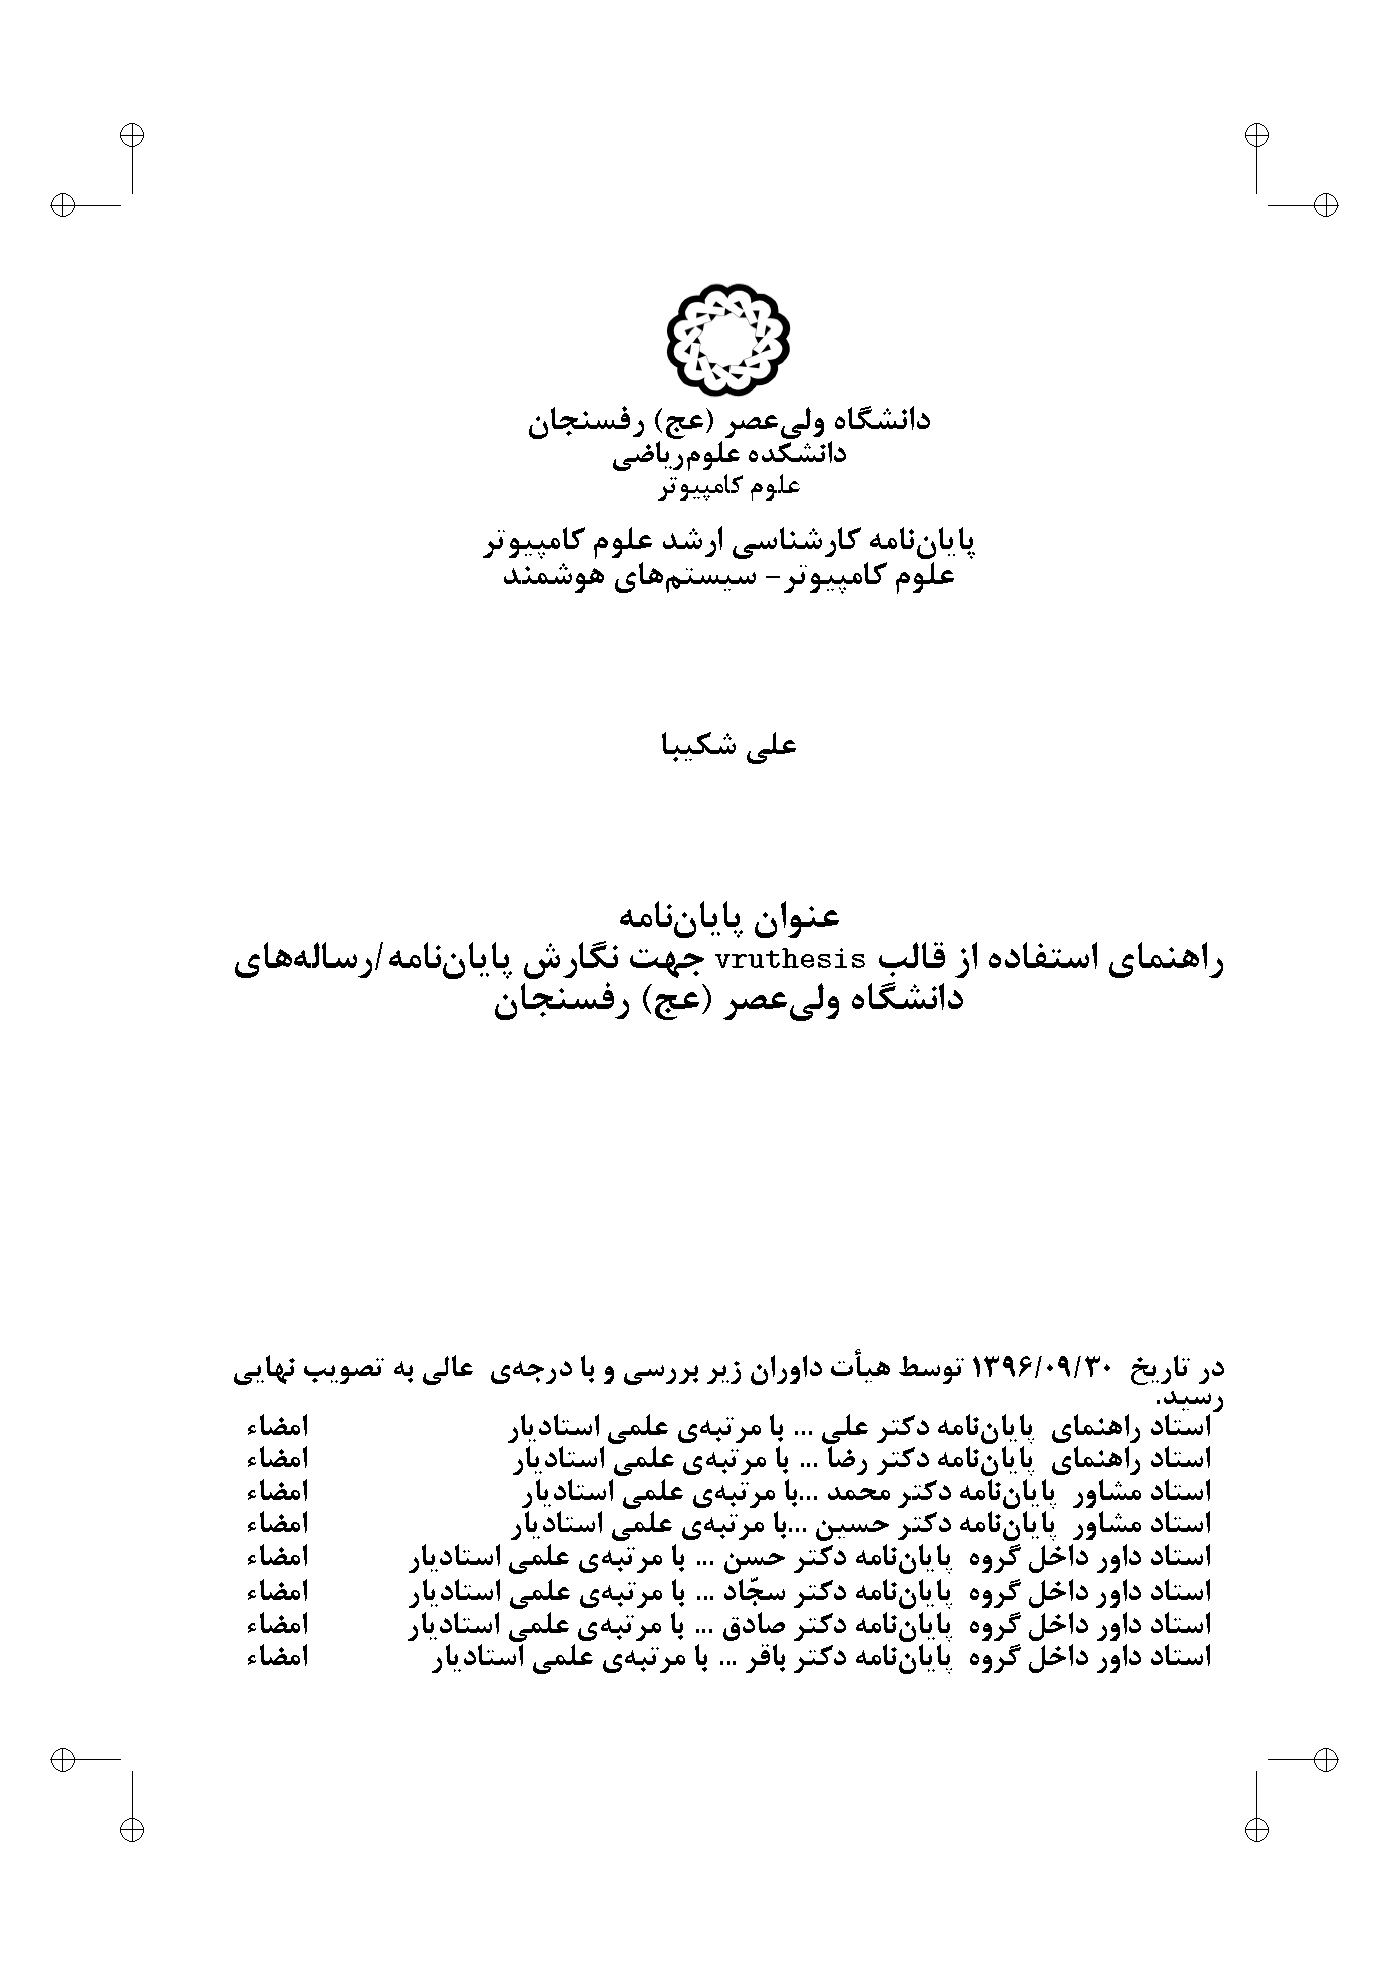
\includegraphics[width=\textwidth]{b.png}
		\caption{نمونه‌ی تصویب‌نامه‌ی پایان‌نامه‌ی کارشناسی ارشد.}
		\label{app2}
	\end{figure}

	\begin{figure}
		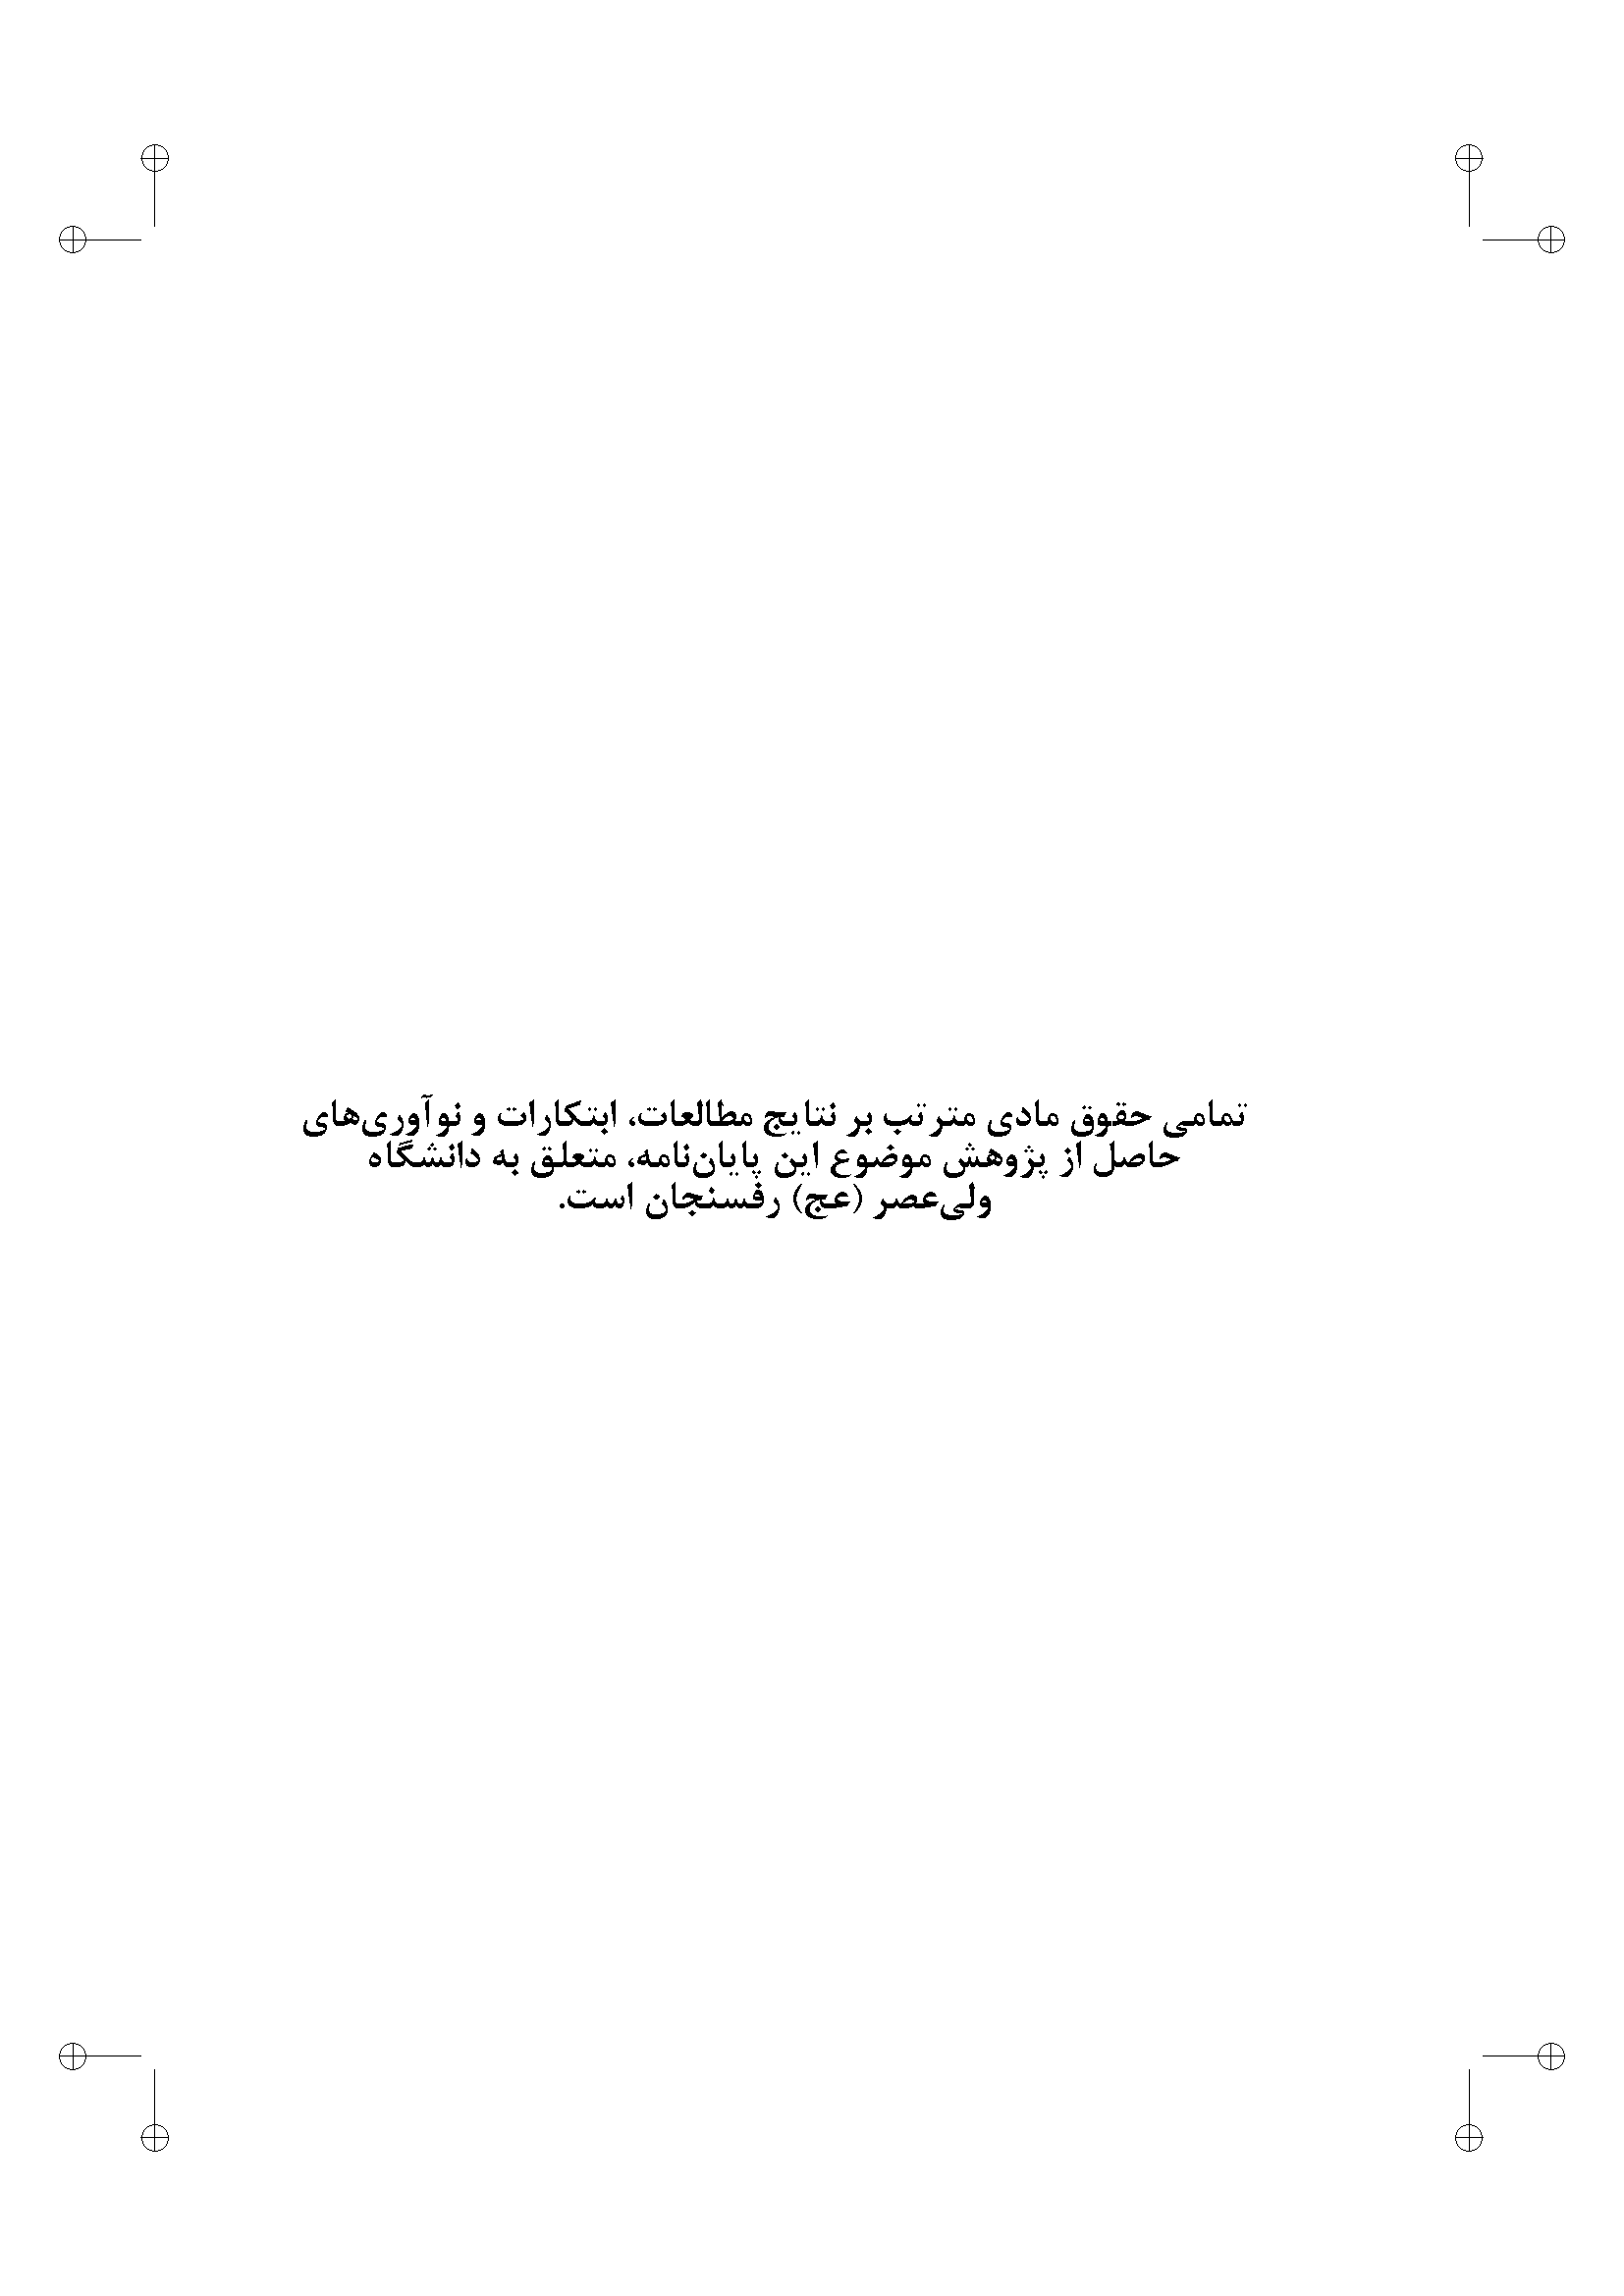
\includegraphics[width=\textwidth]{d.png}
		\caption{تعهدات حقوقی.}
		\label{app4}
	\end{figure}

	\begin{figure}
		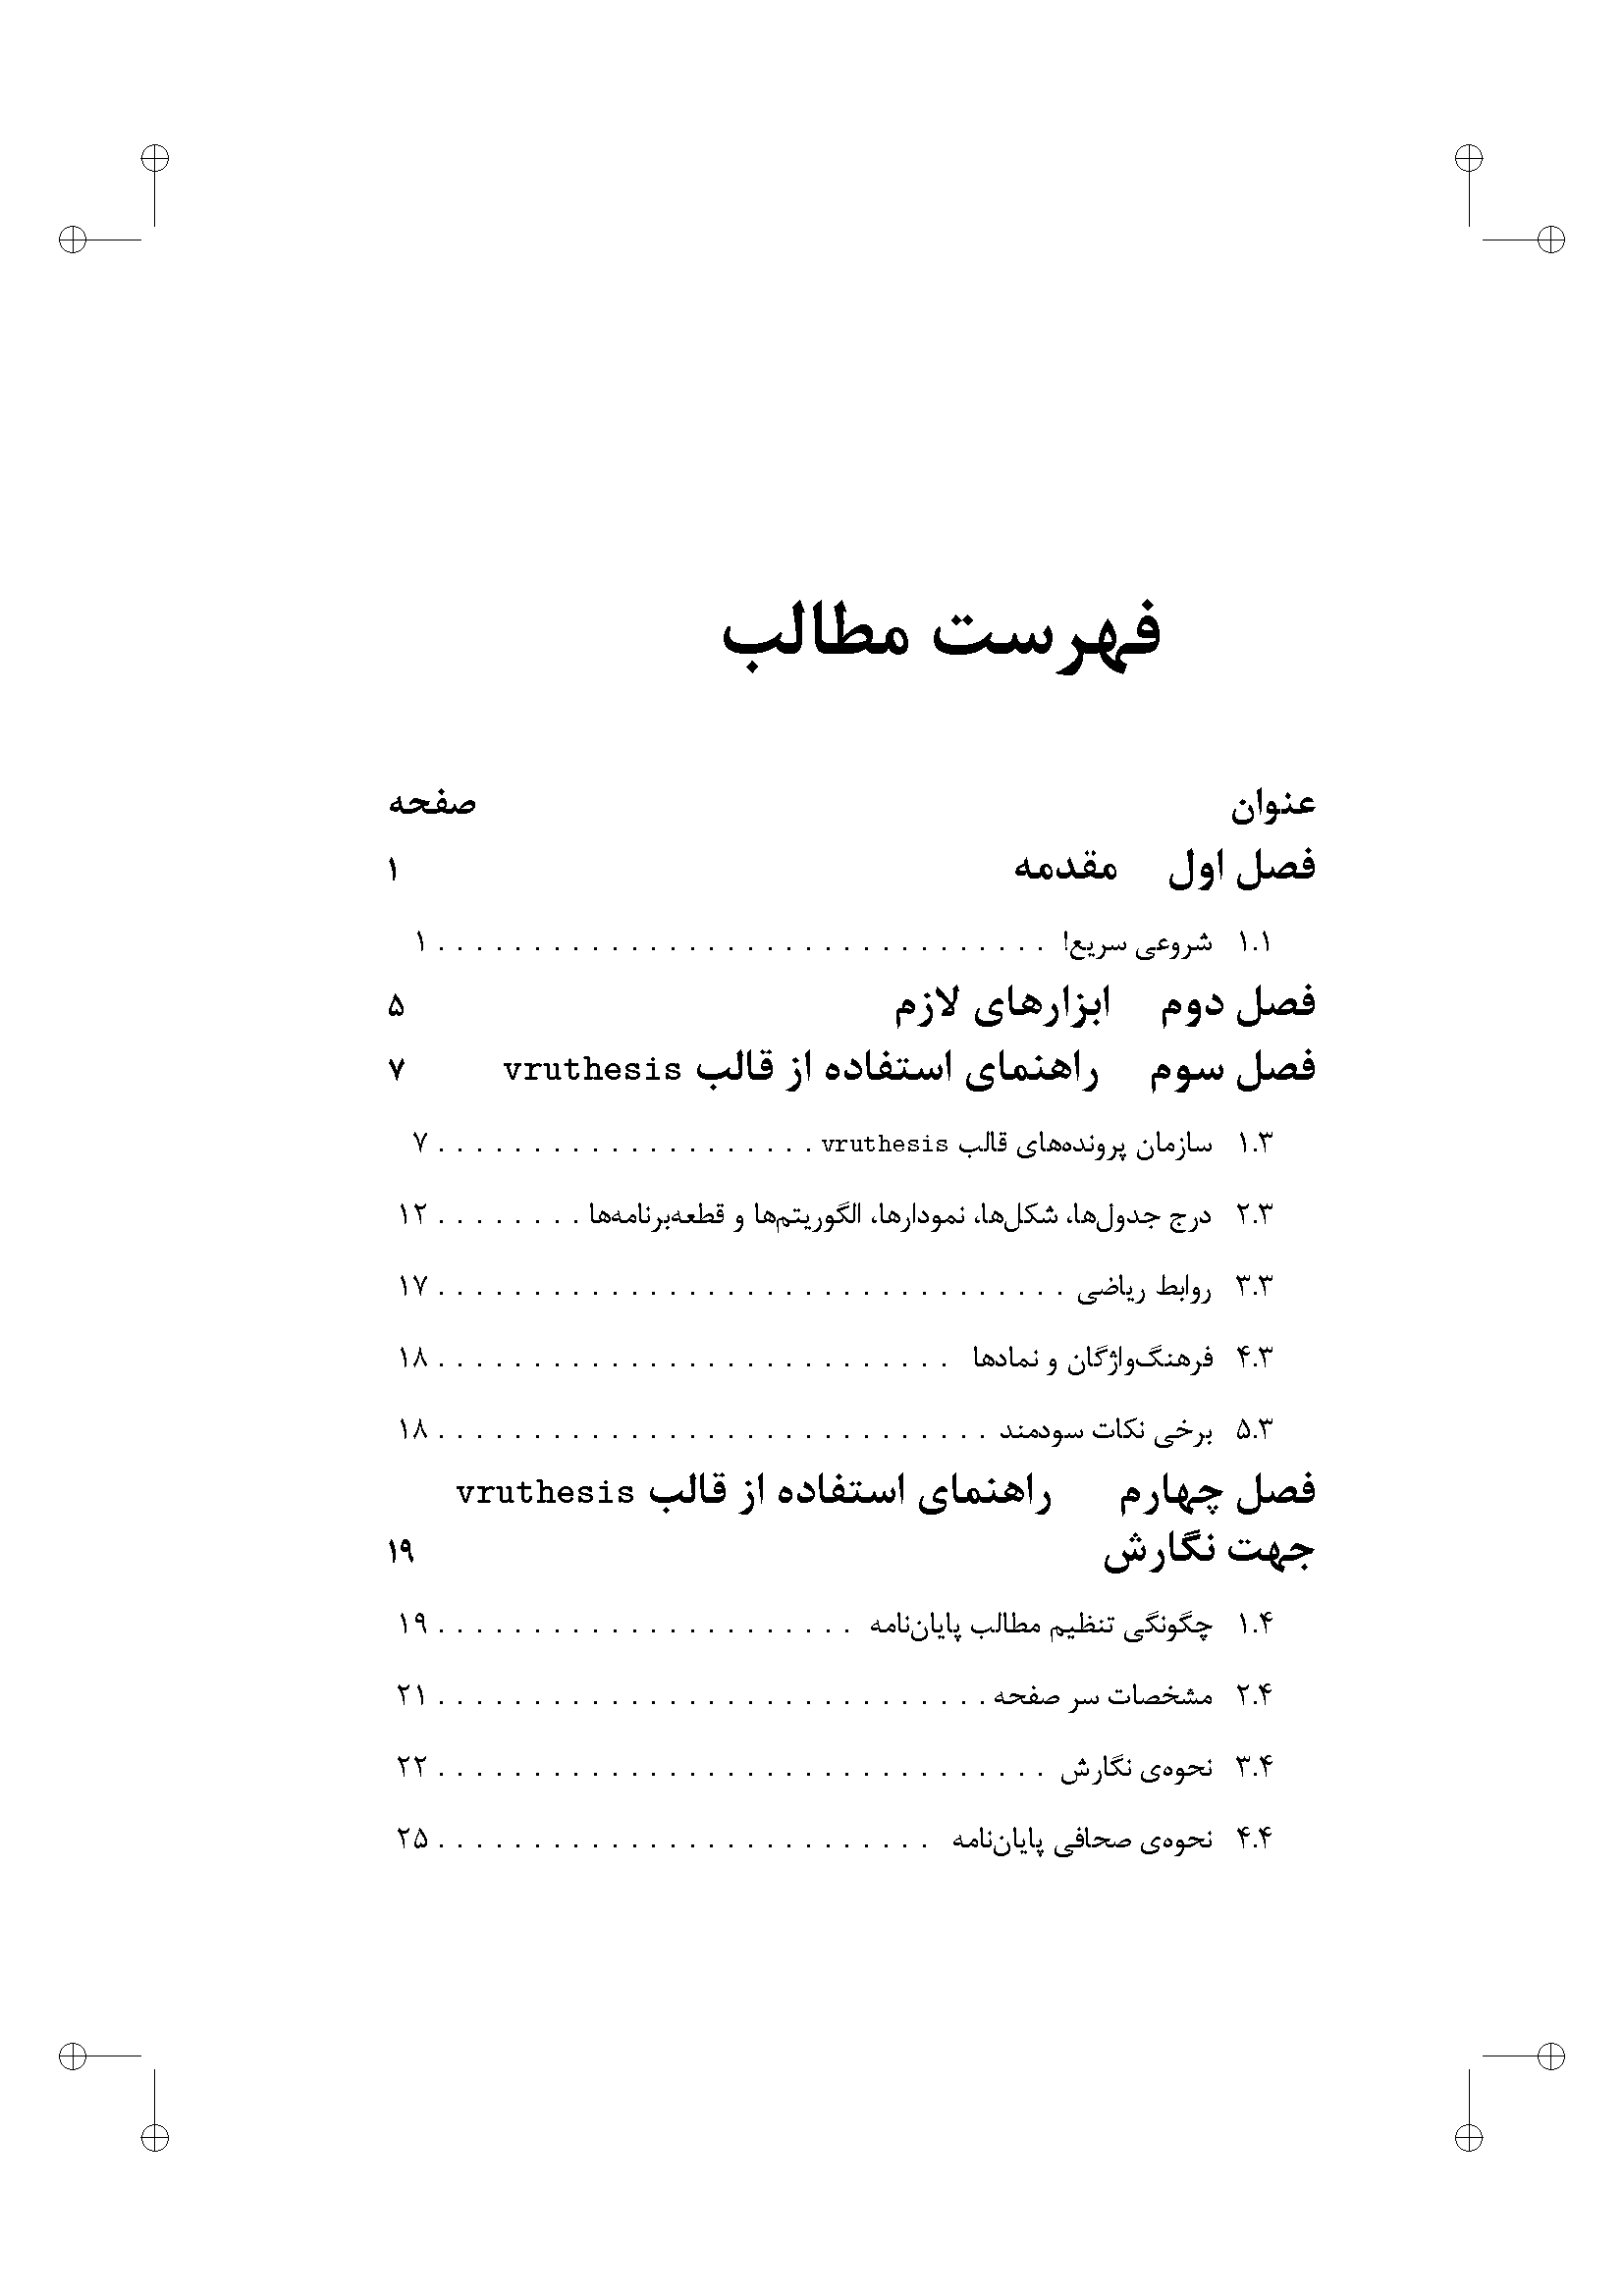
\includegraphics[width=\textwidth]{e.png}
		\caption{نمونه‌ای از فهرست مطالب.}
		\label{app5}
	\end{figure}

	\begin{figure}
		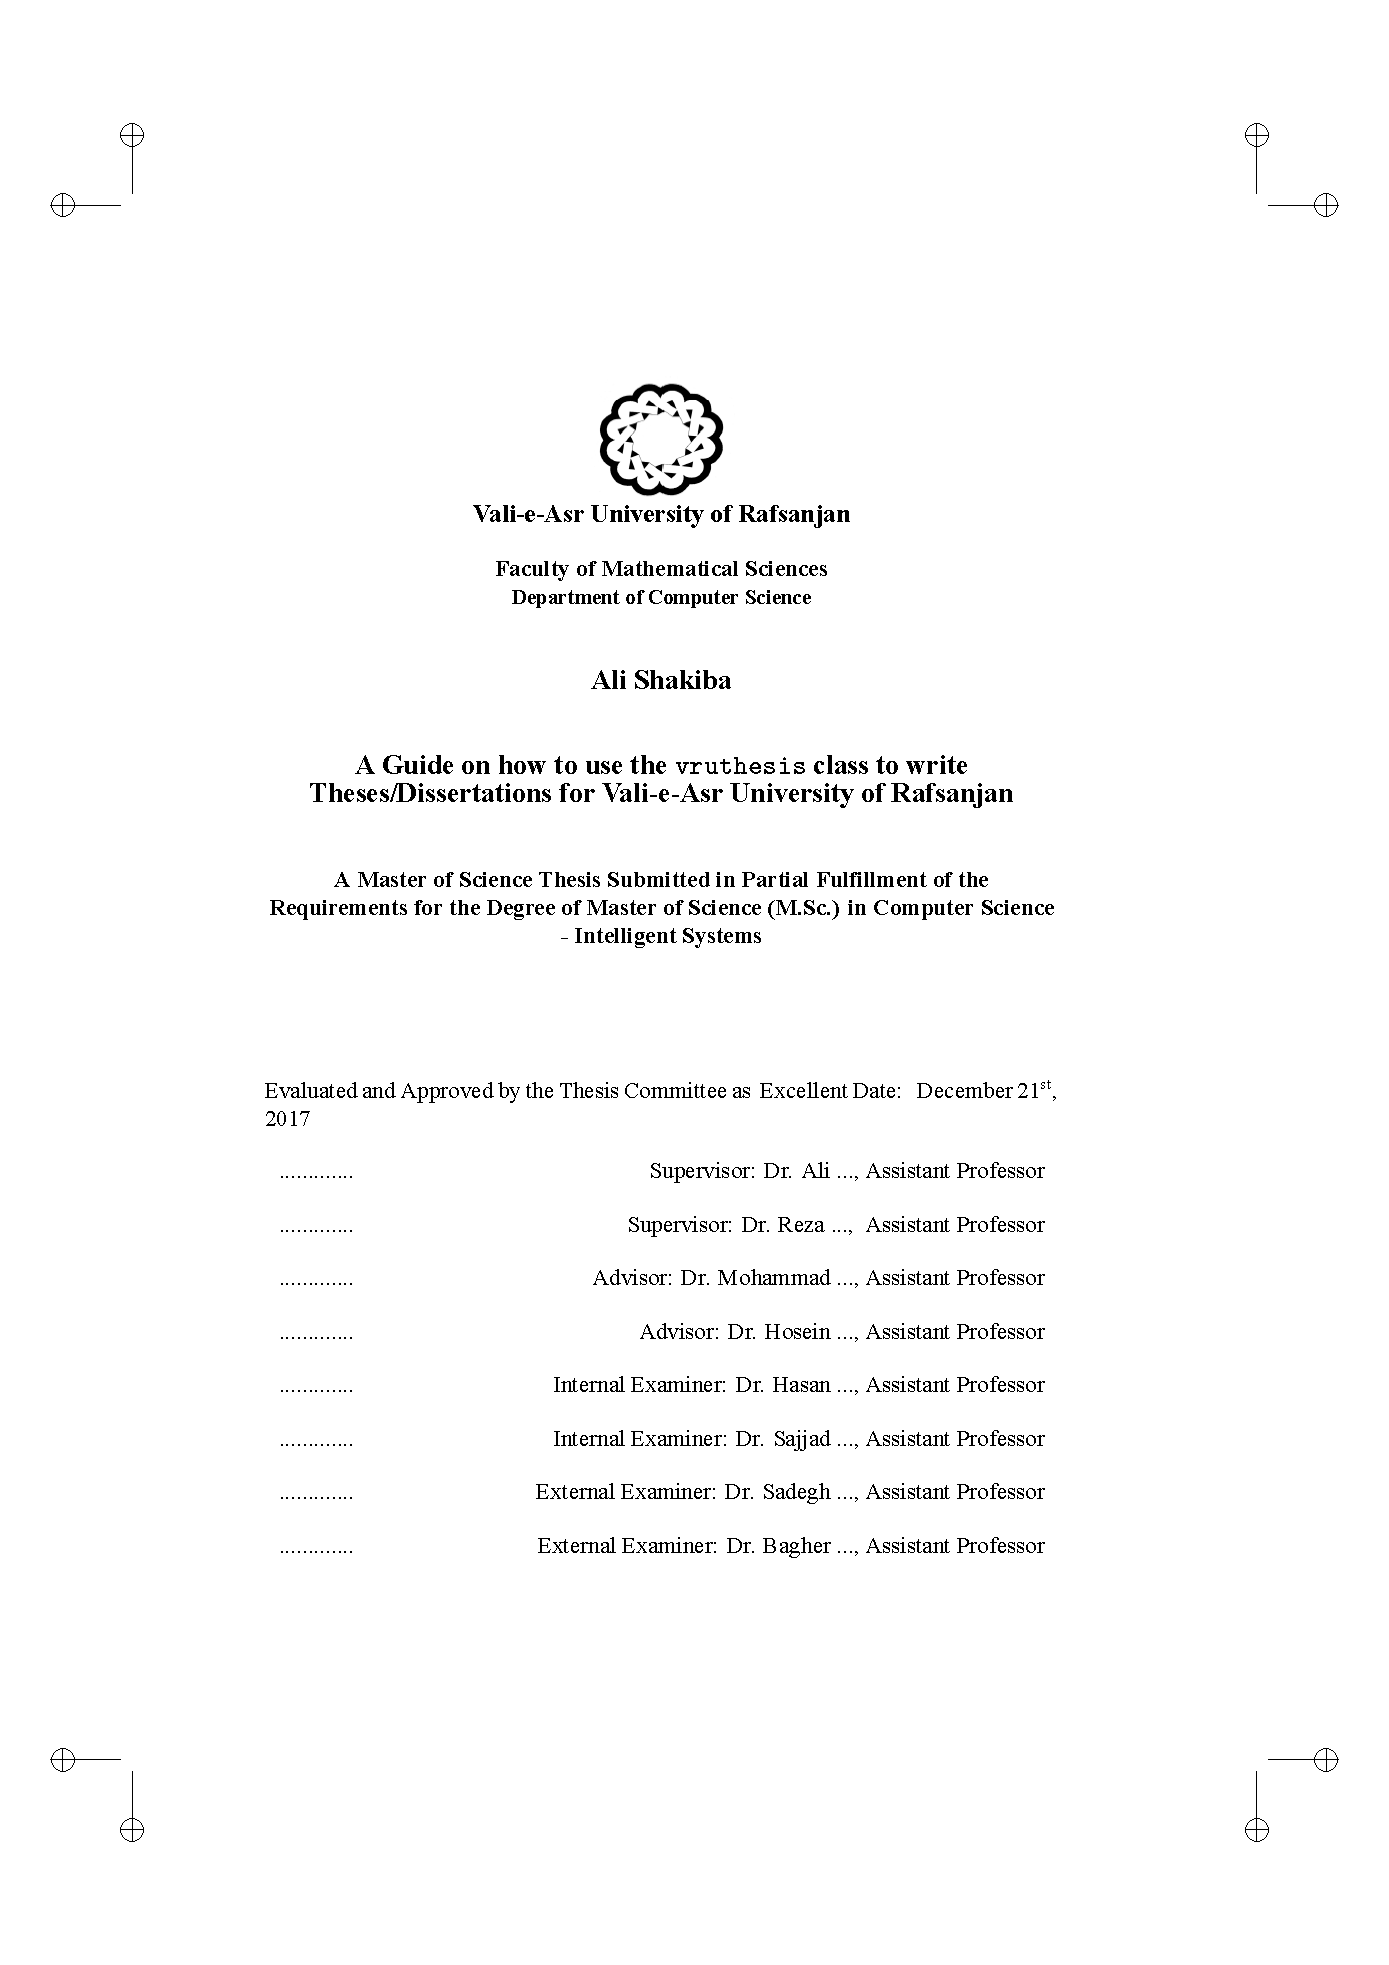
\includegraphics[width=\textwidth]{c.png}
		\caption{نمونه‌ی تصویب‌نامه‌ی پایان‌نامه‌ی کارشناسی ارشد به زبان انگلیسی.}
		\label{app3}
	\end{figure}

	\begin{figure}
		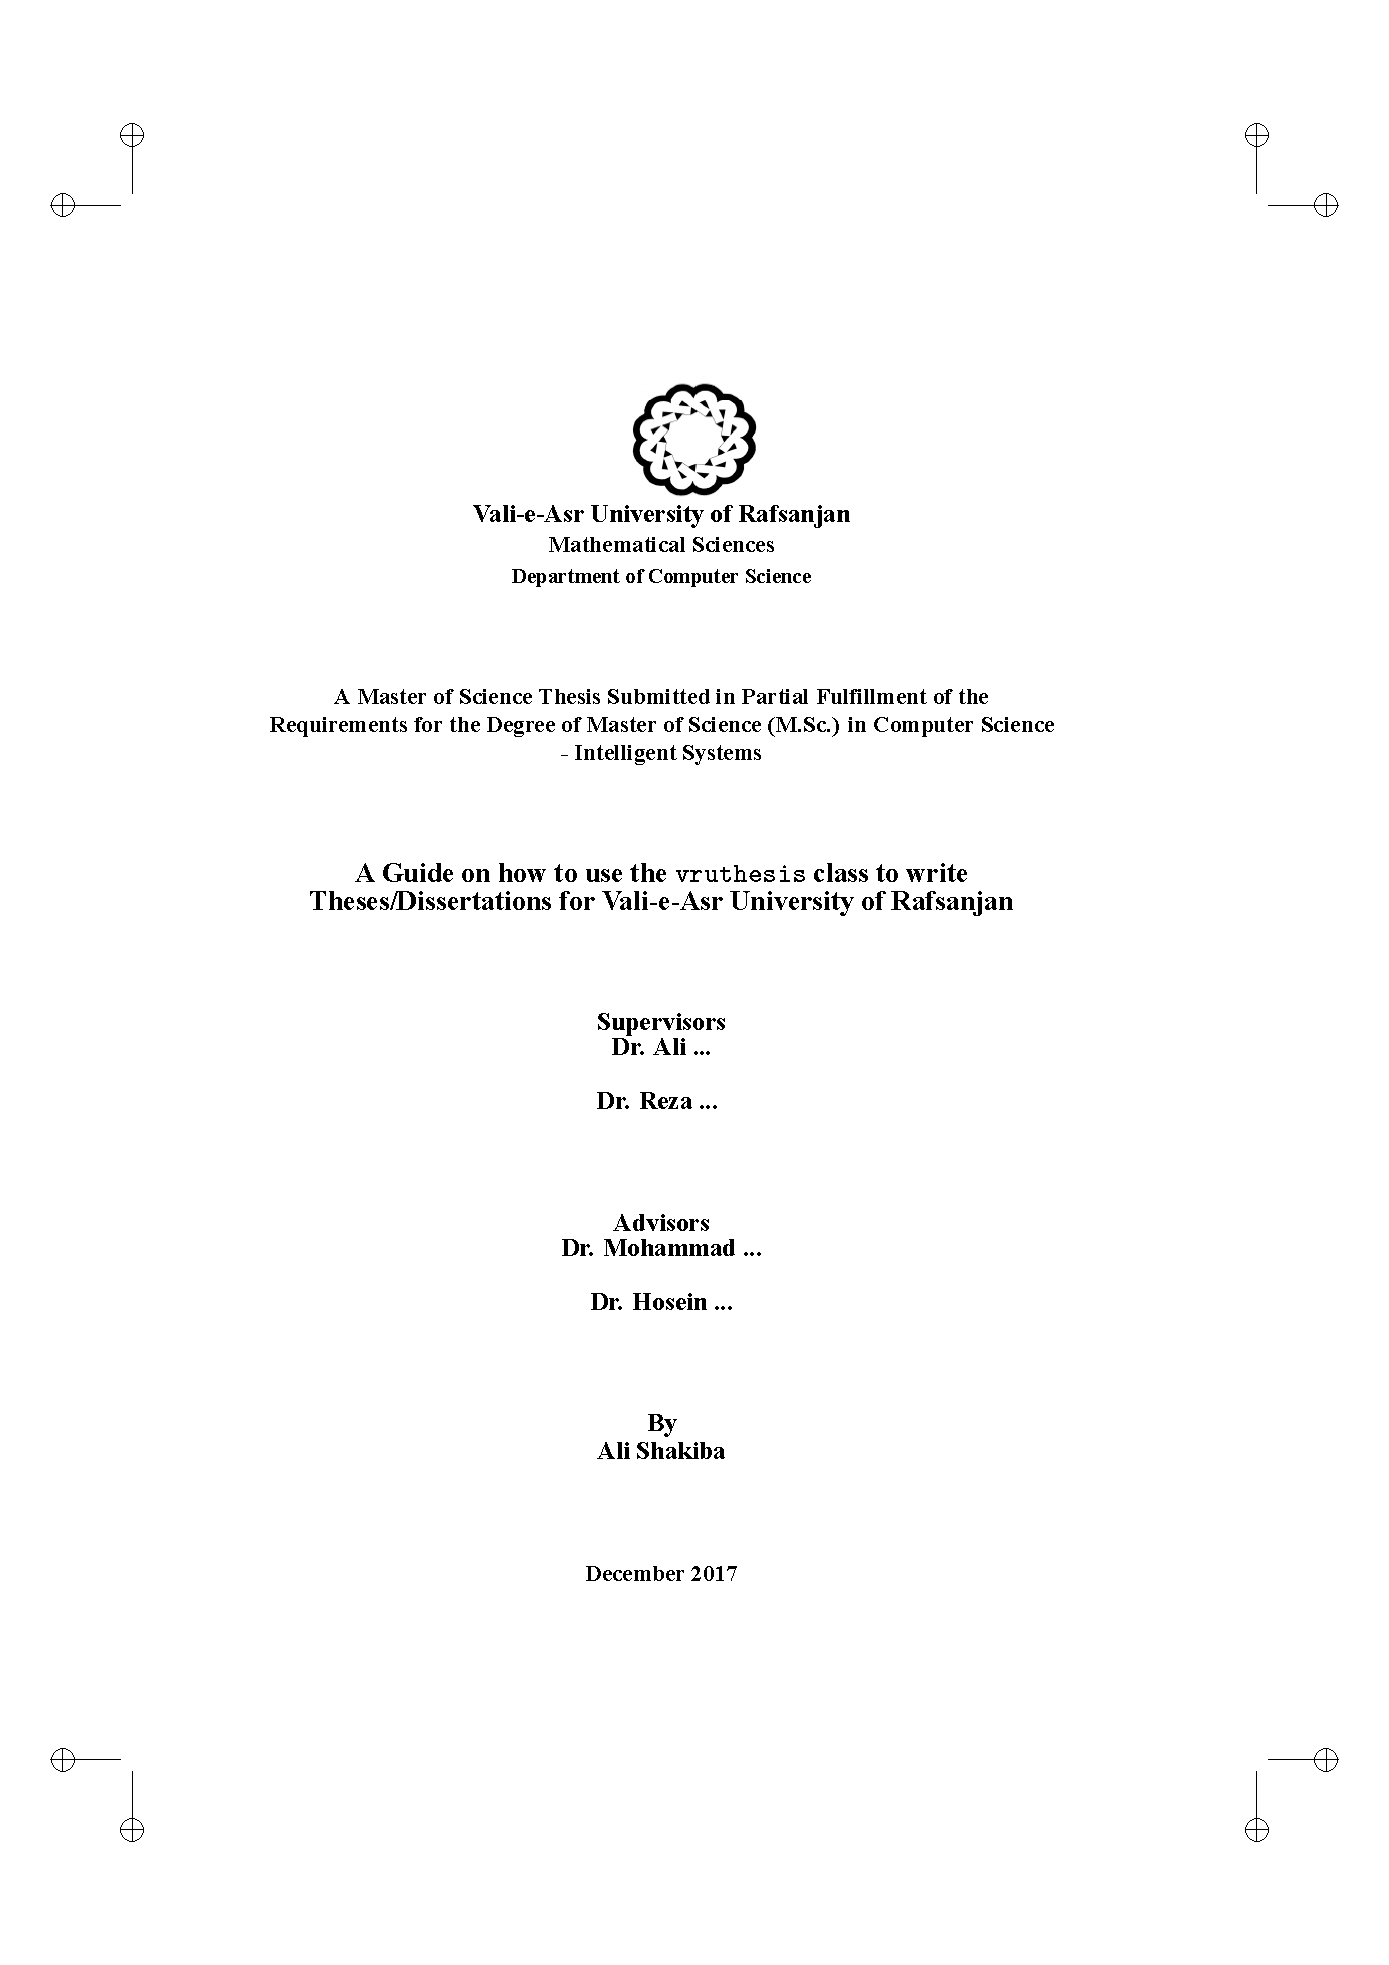
\includegraphics[width=\textwidth]{f.png}
		\caption{نمونه‌ی صفحه‌ی آخر پایان‌نامه‌ی کارشناسی ارشد.}
		\label{app6}
	\end{figure}
| قرار گیرد. 

	جهت تولید صفحات عنوان، ارزیابی، سپاسگزاری، تقدیم‌به و چکیده به هر دو زبان فارسی و انگلیسی، لازم است تا محتوای \gls{file} \texttt{data.tex} را به صورت مناسب، تکمیل کنید. دستورات مورد استفاده در این \gls{file} و کاربرد آن‌ها در جدول \ref{tbl:data_cmds} آمده‌اند. این دستورات ممکن است در نگاه اوّل گیج‌کننده به نظر برسند. به همین دلیل، توصیه می‌شود که از \gls{file} \verb|data.tex| در پایان‌نامه‌ی نمونه استفاده کرده و تنها محتویات خود را در آن، جایگزین نمایید. 
	
	\begin{longtable}[c]{| L{.45\textwidth} | R{.45\textwidth} |}
		\caption{دستورات قابل استفاده در \gls*{file} \texttt{thesis.tex}.}
	\label{tbl:data_cmds}
	\\
	\hline	
		\textbf{شرح} & \textbf{دستور} \\ \hline
	\endfirsthead
	\multicolumn{2}{c}{ادامه‌ی جدول \ref{tbl:data_cmds}.} \\ \hline
	\textbf{شرح} & \textbf{دستور} \\ \hline
	\endhead
		\multicolumn{2}{c}{ادامه‌ی جدول در صفحه‌ی بعد.} \\
	\endfoot
		\hline
	\multicolumn{2}{c}{پایان جدول \ref{tbl:data_cmds}.} \\ 
	\endlastfoot
	
		عنوان دانشکده به فارسی &  \verb|\faculty{}| \\ \hline
		عنوان دانشکده به انگلیسی &  \verb|\facultyen{}| \\ \hline
		نام گروه به فارسی &  \verb|\department{}| \\ \hline
		نام گروه به انگلیسی &  \verb|\departmenten{}| \\ \hline
		عنوان رشته‌ی تحصیلی به فارسی &  \verb|\subject{}| \\ \hline
		عنوان رشته‌ی تحصیلی به انگلیسی &  \verb|\subjecten{}| \\ \hline
		عنوان گرایش تحصیلی به فارسی &  \verb|\field{}| \\ \hline
		عنوان گرایش تحصیلی به انگلیسی &  \verb|\fielden{}| \\ \hline
		عنوان پایان‌نامه به فارسی &  \verb|\title{}| \\ \hline
		عنوان پایان‌نامه به انگلیسی &  \verb|\titleen{}| \\ \hline
		نام و نام خانوادگی استاد راهنما به فارسی با پیشوند «دکتر» &  \verb|\firstsupervisor{}| \\ \hline
		نام و نام خانوادگی استاد راهنما به انگلیسی با پیشوند «\lr{Dr.}» &  \verb|\firstsupervisoren{}| \\ \hline
		رتبه‌ی علمی استاد راهنما به فارسی &  \verb|\firstsupervisorrank{}| \\ \hline
		رتبه‌ی علمی استاد راهنما به انگلیسی &  \verb|\firstsupervisorranken{}| \\ \hline
		نام و نام خانوادگی استاد راهنمای دوم، در صورت وجود، به فارسی با پیشوند «دکتر» &  \verb|\secondsupervisor{}| \\ \hline
		نام و نام خانوادگی استاد راهنمای دوم، در صورت وجود، به انگلیسی با پیشوند «\lr{Dr.}» &  \verb|\secondsupervisoren{}| \\ \hline
		رتبه‌ی علمی استاد راهنمای دوم، در صورت وجود، به فارسی &  \verb|\secondsupervisorrank{}| \\ \hline
		رتبه‌ی علمی استاد راهنمای دوم، در صورت وجود، به انگلیسی &  \verb|\secondsupervisorranken{}| \\ \hline
		نام و نام خانوادگی استاد مشاور، در صورت وجود، به فارسی با پیشوند «دکتر» &  \verb|\firstadvisor{}| \\ \hline
		نام و نام خانوادگی استاد مشاور، در صورت وجود، به انگلیسی با پیشوند «\lr{Dr.}» &  \verb|\firstadvisoren{}| \\ \hline
		رتبه‌ی علمی استاد مشاور، در صورت وجود، به فارسی &  \verb|\firstadvisorrank{}| \\ \hline
		رتبه‌ی علمی استاد مشاور، در صورت وجود، به انگلیسی &  \verb|\firstadvisorranken{}| \\ \hline
		نام و نام خانوادگی استاد مشاور دوم، در صورت وجود، به فارسی با پیشوند «دکتر» &  \verb|\secondadvisor{}| \\ \hline
		نام و نام خانوادگی استاد مشاور دوم، در صورت وجود، به انگلیسی با پیشوند «\lr{Dr.}» &  \verb|\secondadvisoren{}| \\ \hline
		رتبه‌ی علمی استاد مشاور دوم، در صورت وجود، به فارسی &  \verb|\secondadvisorrank{}| \\ \hline
		رتبه‌ی علمی استاد مشاور دوم، در صورت وجود، به انگلیسی &  \verb|\secondadvisorranken{}| \\ \hline
		نام و نام خانوادگی استاد داور داخلی اول به فارسی با پیشوند «دکتر» &  \verb|\firstinternalreferee{}| \\ \hline
		نام و نام خانوادگی استاد داور داخلی اول به انگلیسی با پیشوند «\lr{Dr.}» &  \verb|\firstinternalrefereeen{}| \\ \hline
		رتبه‌ی علمی استاد داور داخلی اول به فارسی &  \verb|\firstinternalrefereerank{}| \\ \hline
		رتبه‌ی علمی استاد داور داخلی اول به انگلیسی &  \verb|\firstinternalrefereeranken{}| \\ \hline
		نام و نام خانوادگی استاد داور داخلی دوم، در صورت وجود، به فارسی با پیشوند «دکتر» &  \verb|\secondinternalreferee{}| \\ \hline
		نام و نام خانوادگی استاد داور داخلی دوم، در صورت وجود، به انگلیسی با پیشوند «\lr{Dr.}» &  \verb|\secondinternalrefereeen{}| \\ \hline
		رتبه‌ی علمی استاد داور داخلی دوم، در صورت وجود، به فارسی &  \verb|\secondinternalrefereerank{}| \\ \hline
		رتبه‌ی علمی استاد داور داخلی دوم، در صورت وجود، به انگلیسی &  \verb|\secondinternalrefereeranken{}| \\ \hline
		نام و نام خانوادگی استاد داور خارجی اول به فارسی با پیشوند «دکتر» &  \verb|\firstexternalreferee{}| \\ \hline
		نام و نام خانوادگی استاد داور خارجی اول به انگلیسی با پیشوند «\lr{Dr.}» &  \verb|\firstexternalrefereeen{}| \\ \hline
		رتبه‌ی علمی استاد داور خارجی اول به فارسی &  \verb|\firstexternalrefereerank{}| \\ \hline
		رتبه‌ی علمی استاد داور خارجی اول به انگلیسی &  \verb|\firstexternalrefereeranken{}| \\ \hline
		نام و نام خانوادگی استاد داور خارجی دوم، در صورت وجود، به فارسی با پیشوند «دکتر» &  \verb|\secondexternalreferee{}| \\ \hline
		نام و نام خانوادگی استاد داور خارجی دوم، در صورت وجود، به انگلیسی با پیشوند «\lr{Dr.}» &  \verb|\secondexternalrefereeen{}| \\ \hline
		رتبه‌ی علمی استاد داور خارجی دوم، در صورت وجود، به فارسی &  \verb|\secondexternalrefereerank{}| \\ \hline
		رتبه‌ی علمی استاد داور خارجی دوم، در صورت وجود، به انگلیسی &  \verb|\secondexternalrefereeranken{}| \\ \hline
		نام و نام خانوادگی استاد ناظر به فارسی با پیشوند «دکتر» &  \verb|\viewer{}| \\ \hline
		نام و نام خانوادگی استاد ناظر به انگلیسی با پیشوند «\lr{Dr.}» &  \verb|\vieweren{}| \\ \hline
		رتبه‌ی علمی استاد ناظر به فارسی &  \verb|\viewerrank{}| \\ \hline
		رتبه‌ی علمی استاد ناظر به انگلیسی &  \verb|\viewerranken{}| \\ \hline
		نام دانشجو به فارسی &  \verb|\name{}| \\ \hline
		نام دانشجو به انگلیسی &  \verb|\nameen{}| \\ \hline
		نام خانوادگی دانشجو به فارسی &  \verb|\surname{}| \\ \hline
		نام خانوادگی دانشجو به انگلیسی &  \verb|\surnameen{}| \\ \hline
		ماه و سال جلسه‌ی دفاع به تقویم شمسی، مانند آذر $1396$ &  \verb|\thesisdate{}| \\ \hline
		ماه و سال جلسه‌ی دفاع به تقویم میلادی، مانند \lr{December 2017} &  \verb|\thesisdateen{}| \\ \hline
		تعداد واحد پایان‌نامه به فارسی، مانند $6$ &  \verb|\credit{}| \\ \hline
		تعداد واحد پایان‌نامه به انگلیسی، مانند \lr{$6$} &  \verb|\crediten{}| \\ \hline
		تاریخ جلسه‌ی دفاع به تقویم شمسی، مانند $۱۳۹۶/۰۹/۳۰$ &  \verb|\defensedate{}| \\ \hline
		تاریخ جلسه‌ی دفاع به تقویم میلادی، مانند \lr{December 21${}^{\text{st}}$, 2017}  &  \verb|\defensedateen{}| \\ \hline
		نمره‌ی پایان‌نامه با اعداد فارسی مانند، $19.75$ &  \verb|\grade{}| \\ \hline
		نمره‌ی پایان‌نامه با اعداد انگلیسی مانند، \lr{$19.75$} &  \verb|\gradeen{}| \\ \hline
		نمره‌ی پایان‌نامه به حروف به زبان فارسی &  \verb|\letgrade{}| \\ \hline
		نمره‌ی پایان‌نامه به حروف به زبان انگلیسی  &  \verb|\letgradeen{}| \\ \hline
		درجه‌ی دفاع به فارسی &  \verb|\degree{}| \\ \hline
		درجه‌ی دفاع به انگلیسی &  \verb|\degreeen{}| \\ \hline
		متن تقدیم‌به به زبان فارسی &  \verb|\totext{}| \\ \hline
		متن سپاسگزاری به فارسی &  \verb|\ack{}| \\ \hline
		متن چکیده به فارسی &  \verb|\abstractfa{}| \\ \hline
		متن چکیده به انگلیسی &  \verb|\abstracten{}| \\ \hline
	\end{longtable}

		\section{درج جدول‌ها، شکل‌ها، نمودارها، الگوریتم‌ها و قطعه‌برنامه‌ها}\label{sec:figs_tbls_algs_codes}
		پایان‌نامه‌ی شما ممکن است دارای جدول‌ها، شکل‌ها، نمودارها، الگوریتم‌ها و قطعه‌برنامه‌های مختلفی باشد. در این قالب، سه نوع محتوا درنظر گرفته شده است:
		\begin{itemize}
			\item جدول که تنها برای نمایش جدول‌ها استفاده می‌شود.
				\item الگوریتم که تنها برای نمایش الگوریتم‌ها استفاده می‌شود. 
			\item شکل که برای نمایش نمودارها،  قطعه‌برنامه‌ها، \glspl{flowchart} و سایر موارد بصری مورد استفاده قرار می‌گیرد.
		\end{itemize}
		
		در ادامه، نمونه‌ای از هر یک از موارد فوق آمده است. جدول \ref{tbl1}، یک جدول با تعداد ستون‌های زیاد است که لازم است تا در صفحه‌ای جداگانه درج شود. قطعه کد تولیدکننده‌ی این جدول در شکل \ref{fig:tbl1} آمده است. 
		
			شکل \ref{fig:clus1} نمونه‌ای از یک خوشه‌بندی برای یک دادگان نمونه است. همچنین، الگوریتم \ref{fig:alg} نیز نمونه‌ای از یک الگوریتم را نشان می‌دهد. از شکل‌ها می‌توان به منظور نمایش نمودارها نیز استفاده کرد؛ مانند \ref{fig:chart}. همچنین، شکل \ref{fig:tbl1}، بیانگر یک قطعه‌کد در \lr{\LaTeX} است. 
			
			\begin{figure}
				\centering
				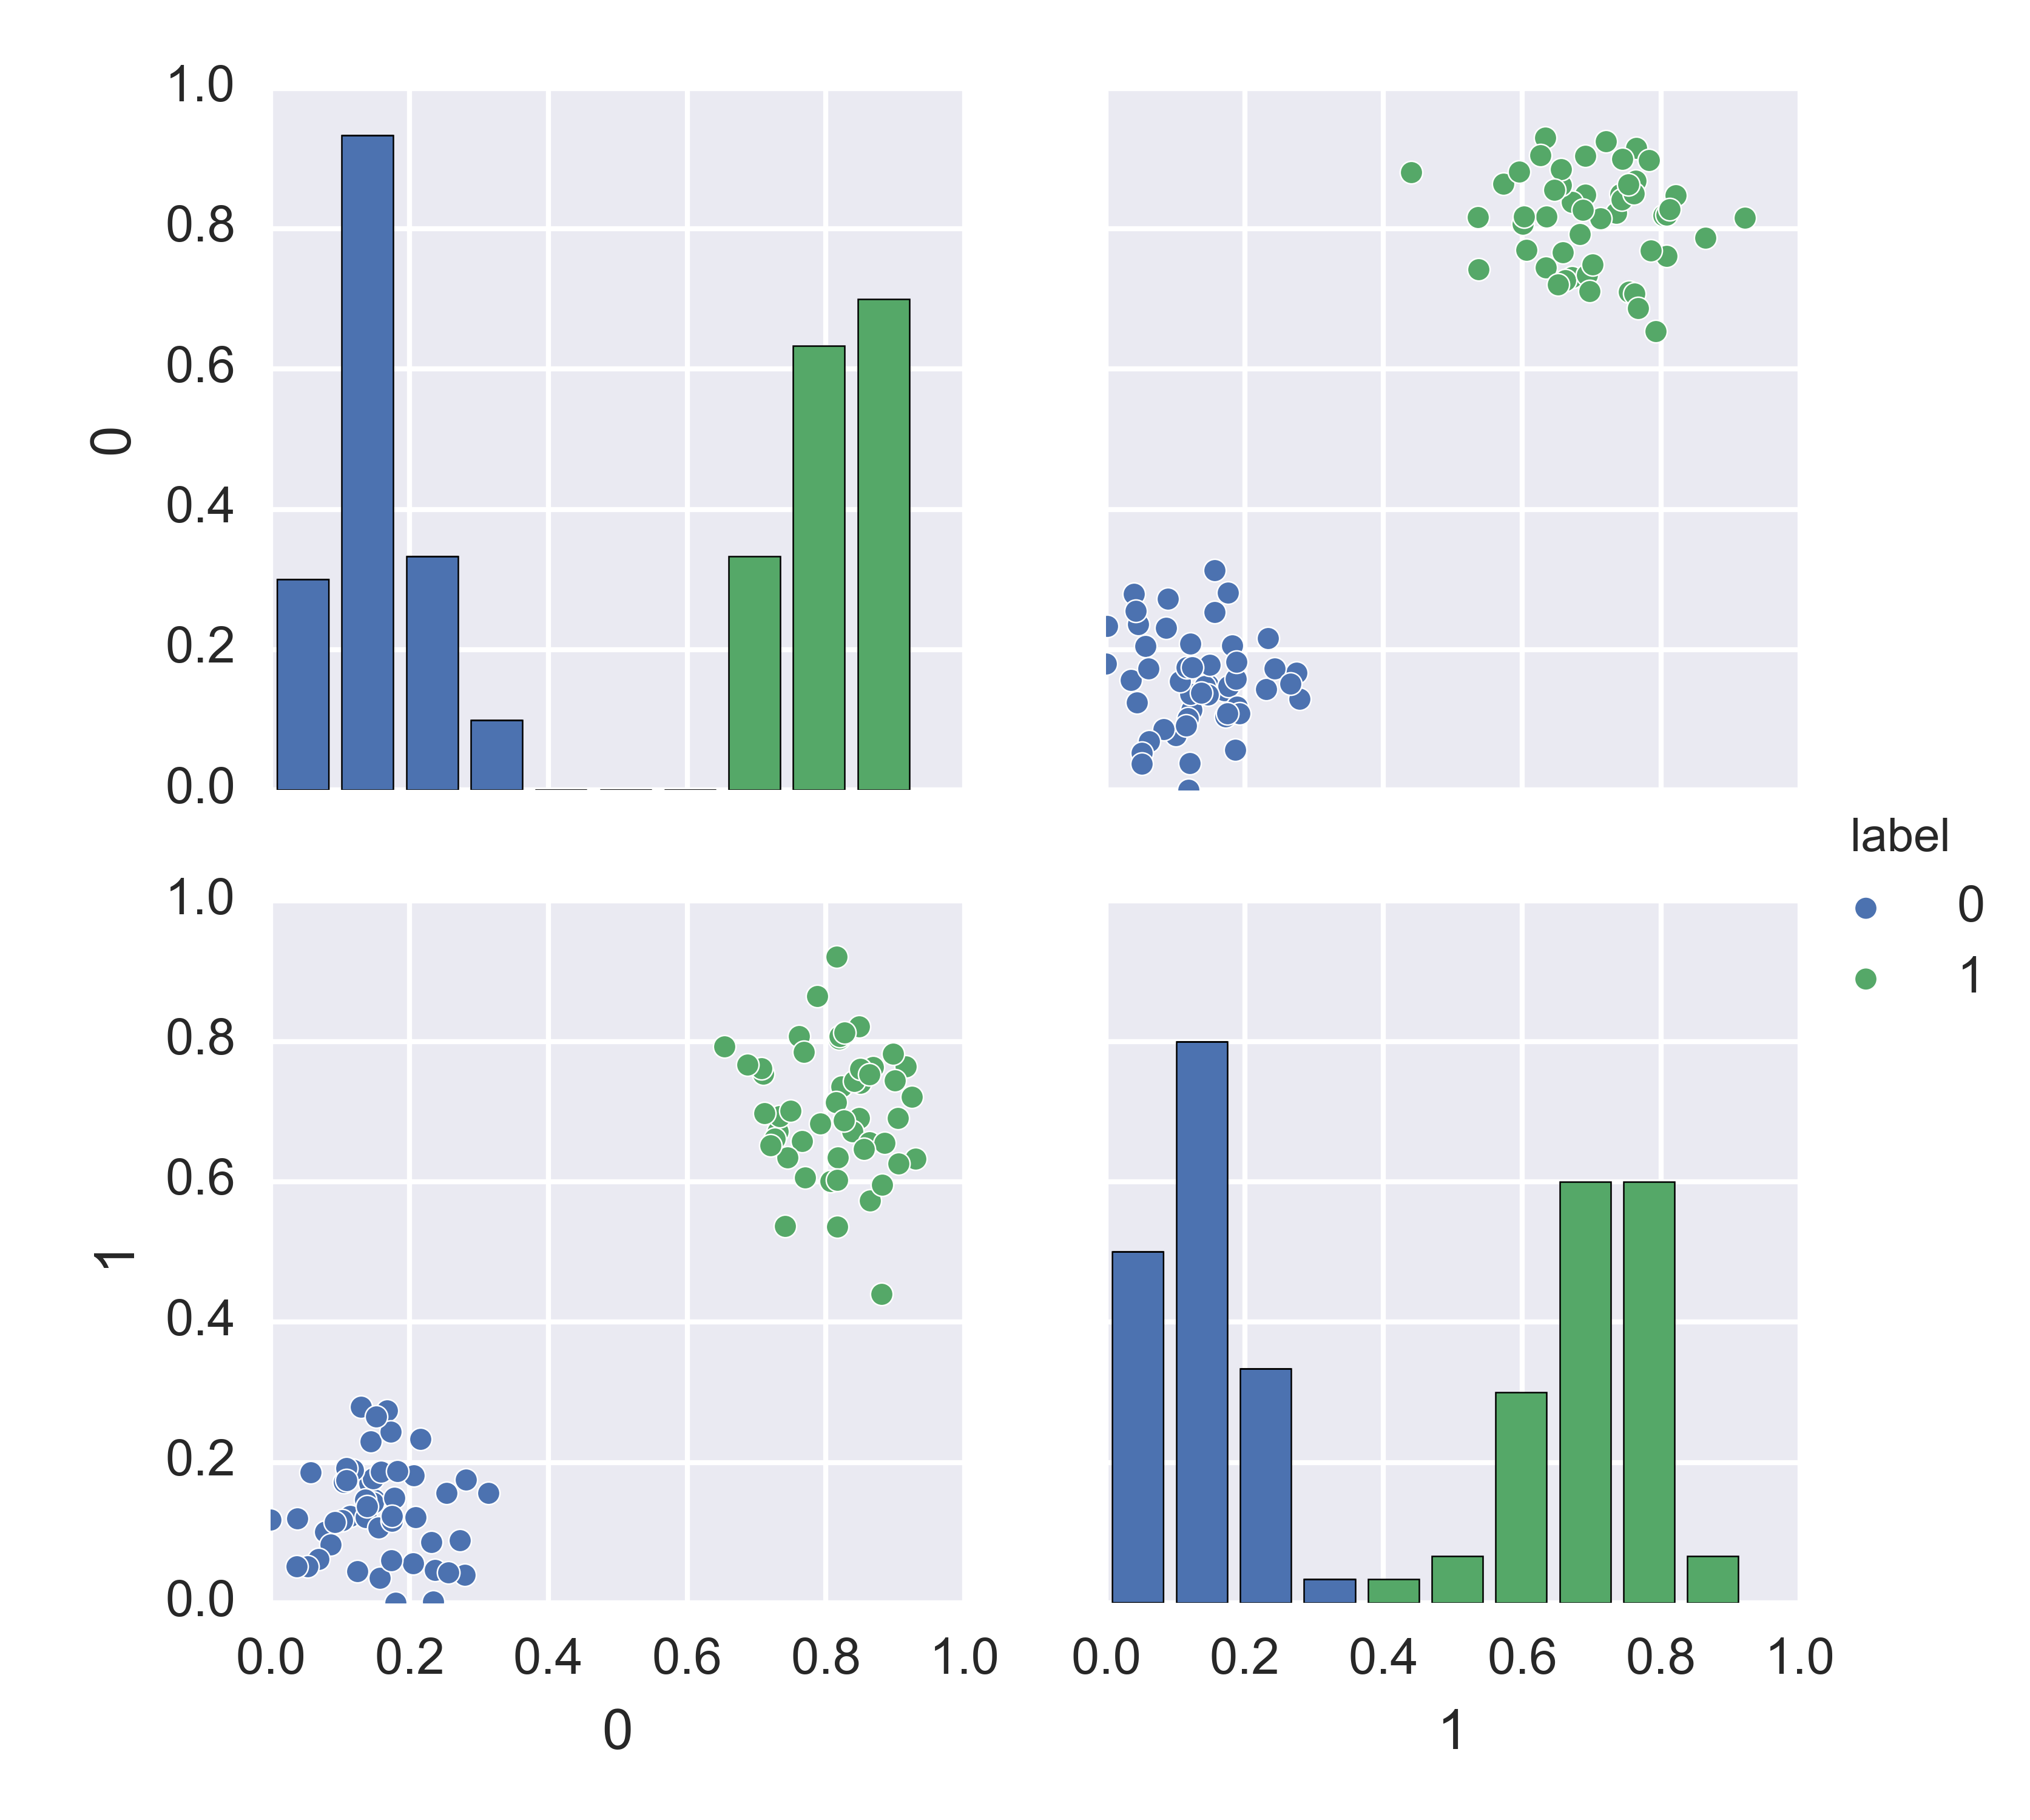
\includegraphics[width=.7\textwidth]{clus1}
				\caption{نمونه‌ای از یک خوشه‌بندی برای یک دادگان نمونه.}
				\label{fig:clus1}
			\end{figure}
		
		\begin{algorithm}
				\begin{latin}
		\begin{algorithmic}[1] % The number tells where the line numbering should start
        \Procedure{Euclid}{$a,b$} \Comment{\rl{ب.م.م. دو عدد صحیح مثبت $a$ و $b$}}
            \State $r\gets a \bmod b$
            \While{$r\not=0$} \Comment{\rl{اگر $r$ صفر باشد؛ پاسخ محاسبه شده است.}}
                \State $a \gets b$
                \State $b \gets r$
                \State $r \gets a \bmod b$
            \EndWhile\label{euclidendwhile}
            \State \textbf{return} $b$\Comment{\rl{ب.م.م. برابر با $b$ است.}}
        \EndProcedure
    \end{algorithmic}
    \end{latin}
    		\caption{الگوریتم اقلیدس برای محاسبه‌ی \gls*{gcd}.}
				\label{fig:alg}		
		\end{algorithm}	
			
			\begin{figure}
				\centering
				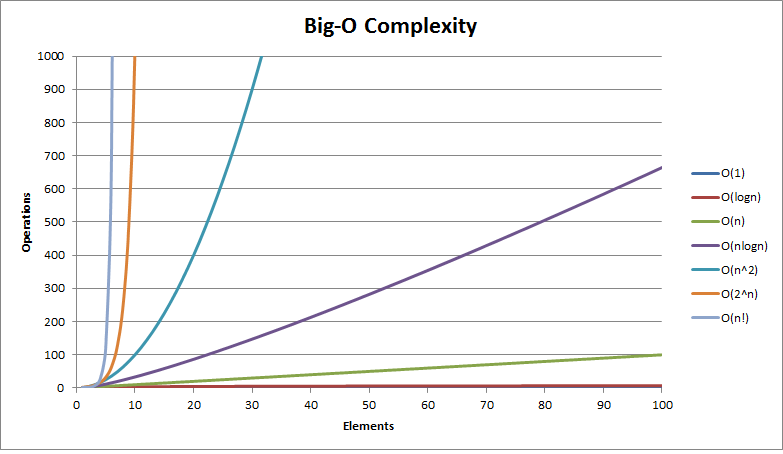
\includegraphics[width=.7\textwidth]{chart}
				\caption{نمونه‌ای از یک نمودار.}
				\label{fig:chart}
			\end{figure}
		
		\begin{figure}
			\centering
		\footnotesize
		\begin{myverbatim}
\begin{landscape}
  \begin{table}
    \caption{+rl[نمونه‌ای از یک جدول با تعداد ستون‌های زیاد.]}
    \label{tbl1}
    \centering
    \footnotesize
    \begin{tabular}{|r||c|c|c|c|c|c|c|c|c|c|c|c|c|c|c|}
      \hline
      \textbf{+rl[عنوان]} & $\alpha$ 
        & \multicolumn{5}{|c|}{$\gamma_1, \gamma_2, \ldots, \gamma_5$} 
        & $\beta$ & \multicolumn{8}{|c|}{+rl[سایر پارامترها]} \\ \hline
      +rl[نمونه‌ی اول]   &   74.85 &  0.32 &  13.99 &  91.25 &  80.74
         &  15.44 &  74.49 &  42.13 &
        1.08  &  32.98 &  18.74 &  46.83 &  81.28 &  31.52 &  8.29 \\
      +rl[نمونه‌ی دوم] &   22.76 &  48.61 &  
        70.77 &  22.77 &  3.81 &  45.05 &  
        70.55 &  33.20 &  1.40  &  24.42 &  79.06 &  
          30.38 &  24.95 &  19.77 &  44.59 \\
      +rl[نمونه‌ی سوم] &   55.67 &  36.98 &
          89.61 &  56.43 &  88.97 &  38.21 &  
        81.40 &  77.05 &  9.35 &  18.52 &  3.48 &  
          95.93 &  9.20 &  16.30 &  84.36 \\
      +rl[نمونه‌ی چهارم] &   60.31 &  88.25 &
          29.96 &  56.83 &  89.49 &  38.26 &  
        55.73 &  99.36 &  21.70 &  74.46 &  49.11 &  2.82
           &  25.47 &  2.90 &  84.58 \\
      +rl[نمونه‌ی پنجم] &   90.17 &  51.53 
        &  32.67 &  82.55 &  87.72 &  66.09 &  26.86 &  
        4.69 &  77.97 &  40.23 &  58.59 &  70.13 &  70.23 &
            80.73 &  64.88 \\
      +rl[نمونه‌ی ششم] &   74.92 
        &  52.33 &  98.68 &  63.75 &  30.10 &  7.32 &  91.70 &  
        72.76 &  42.50 &  26.72 &  23.33 &  73.55 & 
           77.37 &  32.79 &  15.60 \\
      +rl[نمونه‌ی هفتم] &   26.85 &  55.27
         &  5.12 &  88.21 &  4.92 &  70.78 &  
        75.26 &  32.03 &  25.11 &  61.81 &  44.24 &
            47.14 &  98.98 &  16.90 &  20.27 \\
      +rl[نمونه‌ی هشتم] &   84.33 &  12.53 &  36.00
         &  24.02 &  44.60 &  8.44 &  
        5.73 &  10.37 &  16.94 &  15.41 &  39.69 &
            43.74 &  10.43 &  73.96 &  26.51 \\
      +rl[نمونه‌ی نهم] &   59.21 &  47.46 & 
           97.27 &  87.05 &  84.65 &  17.95 &  50.05 &  
        38.68 &  20.09 &  46.99 &  12.47 &  10.92 & 
           78.38 &  74.53 &  31.83 \\
      +rl[نمونه‌ی دهم] &   97.61 &  33.47 &  67.78 
        &  69.95 &  60.95 &  88.40 &  
        59.64 &  18.22 &  57.49 &  97.76 &  40.31 &
            4.83 &  8.90 &  69.18 &  97.02 \\ \hline
    \end{tabular}
  \end{table}
\end{landscape}
		\end{myverbatim}
		\caption{قطعه‌کد مربوط به تولید جدول \ref{tbl1}.}
		\label{fig:tbl1}
		\end{figure}
	
	
		
		\begin{landscape}
			\begin{table}
				\caption{نمونه‌ای از یک جدول با تعداد ستون‌های زیاد.}
				\label{tbl1}
				\centering
				\footnotesize
				\begin{tabular}{|r||c|c|c|c|c|c|c|c|c|c|c|c|c|c|c|}
				\hline
				\textbf{عنوان} & $\alpha$ & \multicolumn{5}{|c|}{$\gamma_1, \gamma_2, \ldots, \gamma_5$} & $\beta$ & \multicolumn{8}{|c|}{سایر پارامترها} \\ \hline
نمونه‌ی اول 	&   74.85 &  0.32 &  13.99 &  91.25 &  80.74 &  15.44 &  74.49 &  42.13 &  1.08  &  32.98 &  18.74 &  46.83 &  81.28 &  31.52 &  8.29 \\
نمونه‌ی دوم &   22.76 &  48.61 &  70.77 &  22.77 &  3.81 &  45.05 &  70.55 &  33.20 &  1.40  &  24.42 &  79.06 &  30.38 &  24.95 &  19.77 &  44.59 \\
نمونه‌ی سوم &   55.67 &  36.98 &  89.61 &  56.43 &  88.97 &  38.21 &  81.40 &  77.05 &  9.35 &  18.52 &  3.48 &  95.93 &  9.20 &  16.30 &  84.36 \\
نمونه‌ی چهارم &   60.31 &  88.25 &  29.96 &  56.83 &  89.49 &  38.26 &  55.73 &  99.36 &  21.70 &  74.46 &  49.11 &  2.82 &  25.47 &  2.90 &  84.58 \\
نمونه‌ی پنجم &   90.17 &  51.53 &  32.67 &  82.55 &  87.72 &  66.09 &  26.86 &  4.69 &  77.97 &  40.23 &  58.59 &  70.13 &  70.23 &  80.73 &  64.88 \\
نمونه‌ی ششم &   74.92 &  52.33 &  98.68 &  63.75 &  30.10 &  7.32 &  91.70 &  72.76 &  42.50 &  26.72 &  23.33 &  73.55 &  77.37 &  32.79 &  15.60 \\
نمونه‌ی هفتم &   26.85 &  55.27 &  5.12 &  88.21 &  4.92 &  70.78 &  75.26 &  32.03 &  25.11 &  61.81 &  44.24 &  47.14 &  98.98 &  16.90 &  20.27 \\
نمونه‌ی هشتم &   84.33 &  12.53 &  36.00 &  24.02 &  44.60 &  8.44 &  5.73 &  10.37 &  16.94 &  15.41 &  39.69 &  43.74 &  10.43 &  73.96 &  26.51 \\
نمونه‌ی نهم &   59.21 &  47.46 &  97.27 &  87.05 &  84.65 &  17.95 &  50.05 &  38.68 &  20.09 &  46.99 &  12.47 &  10.92 &  78.38 &  74.53 &  31.83 \\
نمونه‌ی دهم &   97.61 &  33.47 &  67.78 &  69.95 &  60.95 &  88.40 &  59.64 &  18.22 &  57.49 &  97.76 &  40.31 &  4.83 &  8.90 &  69.18 &  97.02 \\ \hline
				\end{tabular}
			\end{table}
		\end{landscape}
	
		\section{روابط ریاضی}\label{sec:eqs}
		به طور معمول، بخش زیادی از یک پایان‌نامه در دانشکده‌ی علوم ریاضی، از روابط ریاضی تشکیل شده است. یک رابطه‌ی ریاضی را می‌توان به صورت \gls{inline} مانند $\int_{-\infty}^{+\infty} \sin x \mathrm{d} x$ نوشت. همچنین، می‌توان یک رابطه‌ی ریاضی را بدون شماره‌گذاری مانند
		$$
			A \wedge \left( B \vee C \right) = \left(A \wedge B \right) \vee \left( A \wedge C \right),
		$$
		نوشت. امّا، با توجه به زیادبودن تعداد روابط ریاضی، بهتر است در صورتی که به یک رابطه ارجاع داده می‌شود؛ آن را شماره‌گذاری نمایید؛ مانند
		\begin{equation}
			P \left(B_i \vert A \right) = \frac{P\left(A \vert B_i \right) P\left(B_i\right)}{\sum_j P\left(A \vert B_j \right) P\left(B_j\right)},
			\label{eq:1}
		\end{equation}
		که $i=1,\ldots,k$ است. بنابراین، می‌توان به سادگی به رابطه‌ی \ref{eq:1}، ارجاع داد. 
		
		همچنین، محیط‌های متنوعی برای \gls{typeset} قضیه‌ها، لم‌ها، گزاره‌ها، نتیجه‌ها، تعریف‌ها و مانند آن‌ها در نظر گرفته شده‌اند که در ادامه، نمونه‌های مختلفی از آن‌ها را مشاهده می‌کنید.
		
		\begin{theorem}[\cite{gary}]
			\label{}
			زبان $\mathrm{SAT} = \left\{ \left\langle \Phi \right\rangle \ \vert \ \text{\rl{ صدق‌پذیر است} } \Phi  \right\}$، مفروض است. داریم
			\begin{equation}
				\mathrm{SAT} \in \mathbf{NP}\mathrm{-complete}.
			\end{equation}
		\end{theorem}
		\begin{proof}
			برای اثبات می‌توان به مرجع \cite{gary} مراجعه نمود. 
		\end{proof}
		
		\begin{definition}[ضخامت گراف]
			ضخامت گراف $G$ عبارت است از حداقل تعداد گراف‌های مسطح ممکن در تجزیه‌ی $G$ به گراف‌های مسطح.
		\end{definition}
		
		\begin{lemma}{قضیه‌ی پنج رنگ \cite{heawood1890}}
			هر گراف مسطح، قابل $5$-رنگ‌آمیزی است.
		\end{lemma}
		
		\begin{conjecture}[سلام این یک متن است.\cite{ringel1964}]
			درخت $T$ با $m$ یال مفروض است. در این صورت، $K_{2m+1}$ قابل تجزیه به $2m+1$ کپی از $T$ است.
		\end{conjecture}
		
		\begin{problem}
			\gls{bandwidth} گراف $K_{n_1 \ldots n_k}$ را محاسبه نمایید.
		\end{problem}
		
		\begin{proposition}
			ضخامت گراف ساده‌ی $G$ از مرتبه‌ی $n$ و اندازه‌ی $m$، حداقل برابر است با $\frac{m}{3n-6}$.
		\end{proposition}
		
		\begin{corollary}
اندازه‌ی \gls{smallest} و \gls{lmatch} در گراف‌های دوبخشی با یکدیگر برابر است.
		\end{corollary}
		
		\begin{remark}
			نمونه‌های مربوط به گزاره‌ها، قضیه‌ها، تعریف‌ها و مانند آن‌ها در این بخش از مرجع \cite{west} اخذ شده‌اند.
		\end{remark}
		
		\begin{example}
			مثال‌های زیادی از مسائل $\mathbf{NP}\mathrm{-complete}$ وجود دارند؛ مانند $\mathrm{CLIQUE}$.
		\end{example}		
		\section{فرهنگ‌واژگان و نمادها}\label{sec:gloss}
		جهت استفاده از فرهنگ واژگان و نمادها و اختصارات، می‌توانید از دستورات مرتبط استفاده نمایید. قابل ذکر است که قبل از استفاده از یک اختصار یا یک واژه، لازم است تا آن را در یکی از \glspl{file}ی \lr{acronym.tex} یا \lr{gloss.tex} تعریف کنید. در صورتی که واژه یا نماد را به شکل \gls{file} \lr{acronym.tex} تعریف کنید؛ آن واژه در فهرست نماد‌ها و اختصارات درج خواهد شد. همچنین، در صورتی که واژه به شکل \gls{file} \lr{gloss.tex} تعریف شود؛ واژه در فرهنگ واژگان قرار می‌گیرد.
		
		این راهنما به زودی تکمیل می‌گردد.
		\section{برخی نکات سودمند}\label{sec:faq}
			جهت قرارگرفتن تمام مدخل‌های \gls{file} \lr{\texttt{references.bib}}\cite{*} در فهرست مراجع.
	
	\chapter[راهنمای استفاده از قالب \lr{\texttt{vruthesis}} جهت نگارش]{راهنمای استفاده از قالب  جهت نگارش پایان‌نامه‌های دانشگاه ولی‌عصر (عج) رفسنجان}
	در این فصل، گزیده‌ای از «راهنمای استفاده از قالب \lr{\texttt{vruthesis}} جهت نگارش پایان‌نامه/رساله‌های دانشگاه ولی‌عصر (عج) رفسنجان» به نقل از \cite{vru_grad_rules} ذکر می‌گردد. لازم به ذکر است که دستورات مربوط به قالب‌بندی، در این نمونه به صورت دقیق رعایت شده و به تایید شورای تحصیلات تکمیلی دانشکده‌ی ریاضی رسیده است. بنابراین، در صورتی که از این نمونه برای آماده‌سازی پایان‌نامه‌ی خود استفاده می‌کنید؛ نیاز به انجام کار خاصی ندارید.
	\section{چگونگی تنظیم مطالب پایان‌نامه}
		\begin{enumerate}
			\item برگ نخست: سفید
			\item برگ دوم: بسم اللّه الرحمن الرحیم (در وسط صفحه)
			\item برگ سوم: مطابق شکل \ref{app1}
			\item برگ چهارم: تصویب‌نامه‌ی پایان‌نامه به همراه امضای استادان راهنما، مشاور، داور و نماینده‌ی تحصیلات تکمیلی، مطابق با شکل \ref{app2}
			\item پشت برگ چهارم: شکل \ref{app4}
			\item برگ پنجم: سپاس‌گزاری (اختیاری)
			\item پشت برگ پنجم: تقدیم اثر (اختیاری)
			\item مخفف‌ها یا کوتاه‌نوشت‌ها  (در صورت لزوم)
			\item چکیده که شامل هدف، روش پژوهش، نتایج به‌دست آمده و راهکار‌های پیشنهادی برای پژوهش‌های آتی می‌باشد و باید حداقل $200$ کلمه و در یك صفحه و یک پاراگراف، بدون ذکر منابع و شكل باشد. 
			\item فهرست: به‌ترتیب باید فهرست مطالب، شکل‌ها و جدول‌ها ارایه شوند (مطابق با شکل \ref{app5}).
			\item مقدمه (فصل اول): در این قسمت به معرفی پایان‌نامه، فرضیه‌ها و اهداف پژوهش پرداخته می‌شود. (حداکثر در $5$ صفحه).
			\item متن اصلی پایان‌نامه شامل: پیشینه‌ی پژوهش (فصل دوم)، مواد و روش‌ها (فصل سوم)، نتایج و بحث (فصل چهارم) و نتیجه‌گیری کلی و پیشنهادها (فصل پنجم) می‌باشد.
			\item پیوست‌ها: (در صورت وجود)
			\item منابع مورد استفاده: شیوه‌ی نوشتن منابع، مطابق با نمونه‌ی پیشنهادی در پیوست‌ \ref{app7} می‌باشد.
			\item چکیده‌ی انگلیسی: کاملاً منطبق با چکیده‌ی فارسی باشد و به صورت برعکس (از سمت چپ) صحافی شود.
			\item دو برگ ماقبل آخر: مطابق شکل‌های \ref{app3} و \ref{app6} باشند (به‌صورت برعکس صحافی شود)
			\item برگ آخر: صفحه‌ی سفید
		\end{enumerate}
		
		\begin{remark}
			توجه به نکات زیر، حائز اهمیت است:
			\begin{itemize}
				\item در تدوین‌ و تایپ‌ صفحات‌ پایان‌نامه‌ از هیچگونه‌ كادر تزئینی‌ و تذهیب‌ استفاده‌ نگردد.
				\item برای جداسازی فصل‌ها از \lr{break section} استفاده شود تا تمام فصول پشت سر هم در یک فایل موجود باشند. 
				\item پس از اتمام مرحله‌ی حروفچینی و صفحه‌آرایی، متن پایان‌نامه را به‌صورت \gls{pdf} در آورید.
				\item فرمول‌ها به‌صورت ایتالیک تایپ شوند.
			\end{itemize}
		\end{remark}

	\section{مشخصات سر صفحه}
			لازم است در بالای صفحات فرد، عنوان فصل در حاشیه‌ی سمت راست و شماره‌ی صفحه در حاشیه‌ی سمت چپ تایپ شود و در صفحات زوج، عنوان پایان‌نامه در حاشیه‌ی سمت چپ و شماره‌ی صفحه در حاشیه‌ی سمت راست درج شود (مطابق شکل \ref{fig:header}). 
	\begin{figure}
	\centering
	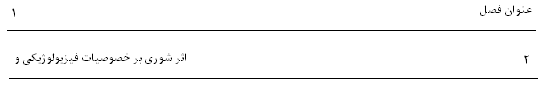
\includegraphics[width=.6\textwidth]{pages.png}
\caption{نمونه‌ای از شیوه‌ی صحیح قرارگیری مشخصات سرصفحه.}
\label{fig:header}
\end{figure}
			\begin{enumerate}[label=\Alph*:]
				\item سرصفحه (\lr{Header}) از صفحه‌ی دوم فصل اول شروع میشود و در صفحه‌ی اول هر فصل، قسمت سرصفحه حذف می‌شود. اول هر فصل باید \lr{break section} در بخش \lr{Page layout} استفاده شود تا سر فصل حذف شود و برای تکرار نشدن سرفصل‌ها در فصل‌های قبلی باید \lr{Link to previous} در بخش \lr{Design} استفاده شود.
				\item متن سرصفحه و شماره‌ی صفحه با قلم  \lr{BNazanin 12 Bold} نوشته شود. 
				\item صفحات سفید، سرصفحه ندارند. 
				\item صفحه‌ی اول فصل، پیوست، نمایه‌ها و واژه‌نامه، سرصفحه ندارند. 
				\item از صفحه‌ی فهرست تا شروع فصل اول، تمامی صفحات با حروف الفبای فارسی و در بالای صفحه، گوشه‌ی خارجی صفحه و به فاصله‌ی 5 سانتی‌متر از بالای كاغذ شماره‌گذاری ‌شود.
				\item از اولین صفحه‌ی فصل اول تا انتهای منابع، تمامی صفحات با اعداد1، 2، 3، و ... در بالای صفحه، گوشه‌ی خارجی صفحه و به فاصله‌ی 5 سانتی‌متر از بالای كاغذ شماره‌گذاری ‌شود.
			\end{enumerate}
			
		\section{نحوه‌ی نگارش}
			نرم‌افزار مورد استفاده برای نگارش پایان‌نامه،  \lr{Microsoft Word 2003} به بالا یا نرم‌افزار مناسب دیگر به تأیید كمیته‌ی تحصیلات تكمیلی دانشکده مربوطه می‌باشد. در صورت استفاده از برنامه \lr{Word}، توجه به نكات زیر ضروری است:  
			\begin{enumerate}%[label=\Alph*:]
				\item متن چکیده‌ی فارسی با قلم \lr{BNazanin 12} و کلمه «چکیده» در اولین خط با قلم \lr{BNazanin 12 Bold} در اول سطر درج شود. 
				\item متن چکیده‌ی انگلیسی با قلم \lr{Times New Roman 11} و کلمه \lr{Abstract} در اولین خط با قلم \lr{Time New Roman 11 Bold} در اول سطر درج شود. 
				\item متن مقدمه با قلم \lr{BNazanin 12} و کلمه «مقدمه» در اولین خط با قلم \lr{Bold  BNazanin 14} در اول سطر درج شود.
				\item متن اصلی پایان‌نامه باید روی دو طرف کاغذ \lr{A4} با قلم \lr{BNazanin 12} و با فاصله خطوط یکسان به صورت (\lr{Single}) نوشته شود. 
				\item در متن اصلی پایان‌نامه، لغات یا حروف انگلیسی (از جمله، منابع انگلیسی) با قلم \lr{Times New Roman 11} نوشته شود.
				\item عناوین فصل‌ها با قلم \lr{14 BNazanin Bold} نوشته شود.
				\item سطر اول تمامی پاراگراف‌های موجود در متن پایان‌نامه، بایستی $0.5$ سانتی‌متر تورفتگی داشته باشند. توجه داشته باشید که عنوان بخش‌ها یا زیر بخش‌ها نبایستی دارای تورفتگی باشند.
				\item قسمت‌های مختلف هر فصل با اعدادی نظیر 6-4- یا 6-4-2- مشخص میشود كه عدد 6 شماره‌ی فصل، عدد4 شماره‌ی بخش و عدد 2 شماره‌ی زیر بخش است. بخش‌های مختلف فصل‌ها با قلم \lr{BNazanin 13 Bold} و زیربخش‌های اول با قلم \lr{BNazanin 12 Bold}  و زیربخش‌های دوم با \lr{BNazanin 11 Bold} تایپ شود.
				\item تمامی شکل‌ها و جدول‌ها باید به ترتیب ظهور در هر فصل شماره‌گذاری شوند. مثلاً برای جدول‌های فصل 2، جدول 2-1، جدول 2-2 و ... برای جدول‌های فصل 3، جدول 3-1، جدول 3-2 و .... عنوان جدول‌ها در بالای آن‌ها و وسط صفحه و عنوان شکل‌ها در زیر آنها، وسط صفحه با قلم \lr{BNazanin 10 Bold}  نوشته شود. اعداد و متن داخل جدول با قلم \lr{BNazanin 10}   نوشته شود. اگر شکلی از مرجعی نقل شده باشد، لازم است مرجع آن در زیر شکل داخل پرانتز آورده شود.
				\item جدول‌هایی که در راستای طولی کاغذ تنظیم میشوند، باید طوری قرار گیرند که متن بالای آنها در سمت لبه‌ی پایان‌نامه واقع شود (درتمامی جدول‌ها خطوط عمودی باید حذف شود). شکل‌ها و جدول‌ها داخل متن و در نزدیکترین فاصله به محل ذکر شده، آورده شوند (حاشیه‌ی شکل‌ها حذف شود). هم‌چنین شکل‌هایی که در راستای طولی کاغذ تنظیم می‌شوند، باید طوری قرار گیرند که متن پایین آنها در سمت لبه‌ی پایان‌نامه قرار گیرد. 
				\item فرمول‌ها (در صورت نیاز به ارجاع) در هر فصل به‌طور جداگانه و به ترتیبی که ظاهر می‌شوند (مانند جدول‌ها و شکل‌ها) شماره‌گذاری می‌گردد (مانند 2-3، 2-4، 3-1 و ...).
				\item معادل انگلیسی لغات یا اصطلاحات فارسی که برای اولین‌بار به کار می‌رود به صورت زیرنویس (فقط برای یک‌بار) با قلم Times New Roman 10 در صفحه‌ی مربوط درج شود. (سعی شود در متن پایان‌نامه‌، از بکار بردن واژه‌های با الفبای انگلیسی خودداری شود). زیرنویس‌ها در هر صفحه با گذاردن شماره‌ی 1، 2 و ... در گوشه‌ی بالای آخرین کلمه در متن مشخص میشوند. زیر نویس باید به شکل زیر در زیر نویس آورده شود. \\
\begin{latin}
\footnotesize	$1$ Water use efficiency
\end{latin}
				\item لازم است در متن به تمامی منابعی كه مورد استفاده قرار می‌گیرند، اشاره شود. چنانچه در داخل متن از یك منبع مطلبی نقل شود، بلافاصله پس از ذكر نام نویسنده و یا در خاتمه‌ی جمله، پرانتزی باز شود و مرجع ذكر گردد. شیوه‌ی نامه‌ی نگارش منابع پیوست شده است (پیوست شماره‌ی \ref{app6}).
				
			\end{enumerate}

		حاشیه‌های صفحات مطابق نمونه‌ی شکل \ref{layout} ($4.5$ سانتیمتر فاصله از بالا و پایین و $4$ سانتیمتر از چپ و $5$ سانتیمتر از راست رعایت گردد (توجه: برای تنظیم این فاصله‌ها از حاشیه از طریق \lr{Page layout} وارد \lr{Page setup} شده و اعداد را با واحد سانتیمتر وارد کنید. در ضمن در همان صفحه در قسمت \lr{Multiple pages} کلمه \lr{mirror margin} را انتخاب کنید تا در صفحات زوج و فرد فاصله متن از حاشیه بیرونی $4$ سانتیمتر و از حاشیه درونی $5$ سانتیمتر شود (در \lr{Page setup} باید سایز (\lr{Size Letter}) انتخاب شود).
		
		\begin{figure}
	\centering
	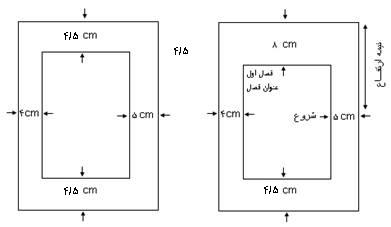
\includegraphics[width=.6\textwidth]{layout.png}
\caption{حاشیه‌ی صفحات.}
\label{layout}
\end{figure}
\section{نحوه‌ی صحافی پایان‌نامه}
	روی جلد مطابق یا پیوست شماره‌ی \ref{app1} تنظیم گردد، عطف آن مانند نمونه‌ی شکل \ref{atf} نوشته می‌شود.
	\begin{figure}
	\centering
	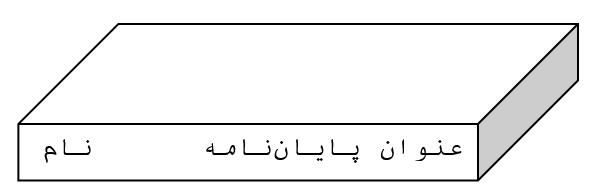
\includegraphics[width=.6\textwidth]{atf.png}
\caption{نمونه‌ای از شیوه‌ی صحیح \gls*{typeset} عطف.}
\label{atf}
\end{figure}
ابعاد پایان نامه بعد از صحافی، $23.5 \times 17$ (قطع وزیری) باید باشد. ابعاد سیاهه متن پایان‌نامه (از بالای متن سرصفحه تا پایین متن اصلی و عرض متن) $18.3 \times 12$ باید باشد. 
فاصله‌ی متن سرصفحه از حاشیه‌ی بالا $2.5$ سانتیمتر و فاصله‌ی متن اصلی از حاشیه‌ی پایین $2.7$ سانتیمتر، فاصله‌ی متن از حاشیه‌ی بیرونی $2$ سانتیمتر و از حاشیه‌ی درونی $3$ سانتیمتر باید باشد.  

رنگ جلد پایان‌نامه‌های کارشناسی‌ارشد کلیه رشته‌ها سورمه‌ای و رساله دکتری سبز یشمی می‌باشد. همچنین، اصل پایان‌نامه قبل از صحافی و پس از تایپ و آماده‌سازی به رؤیت مدیر تحصیلات تكمیلی دانشگاه یا معاون آموزشی دانشكده رسانیده شود و پس از مطابقت با ضوابط مصوب، تأییدیه صادر گردد.


	\chapter{نتیجه‌گیری}
در این فصل، نتیجه‌گیری پایان‌نامه‌ی خود را درج کنید.
			
	\appendix
	\chapter{یک پیوست}
مطالب این پیوست بر اساس راهنمای نگارش پایان‌نامه‌های تحصیلات تکمیلی در \cite{vru_grad_rules} تهیه شده‌اند. 

	\begin{figure}
		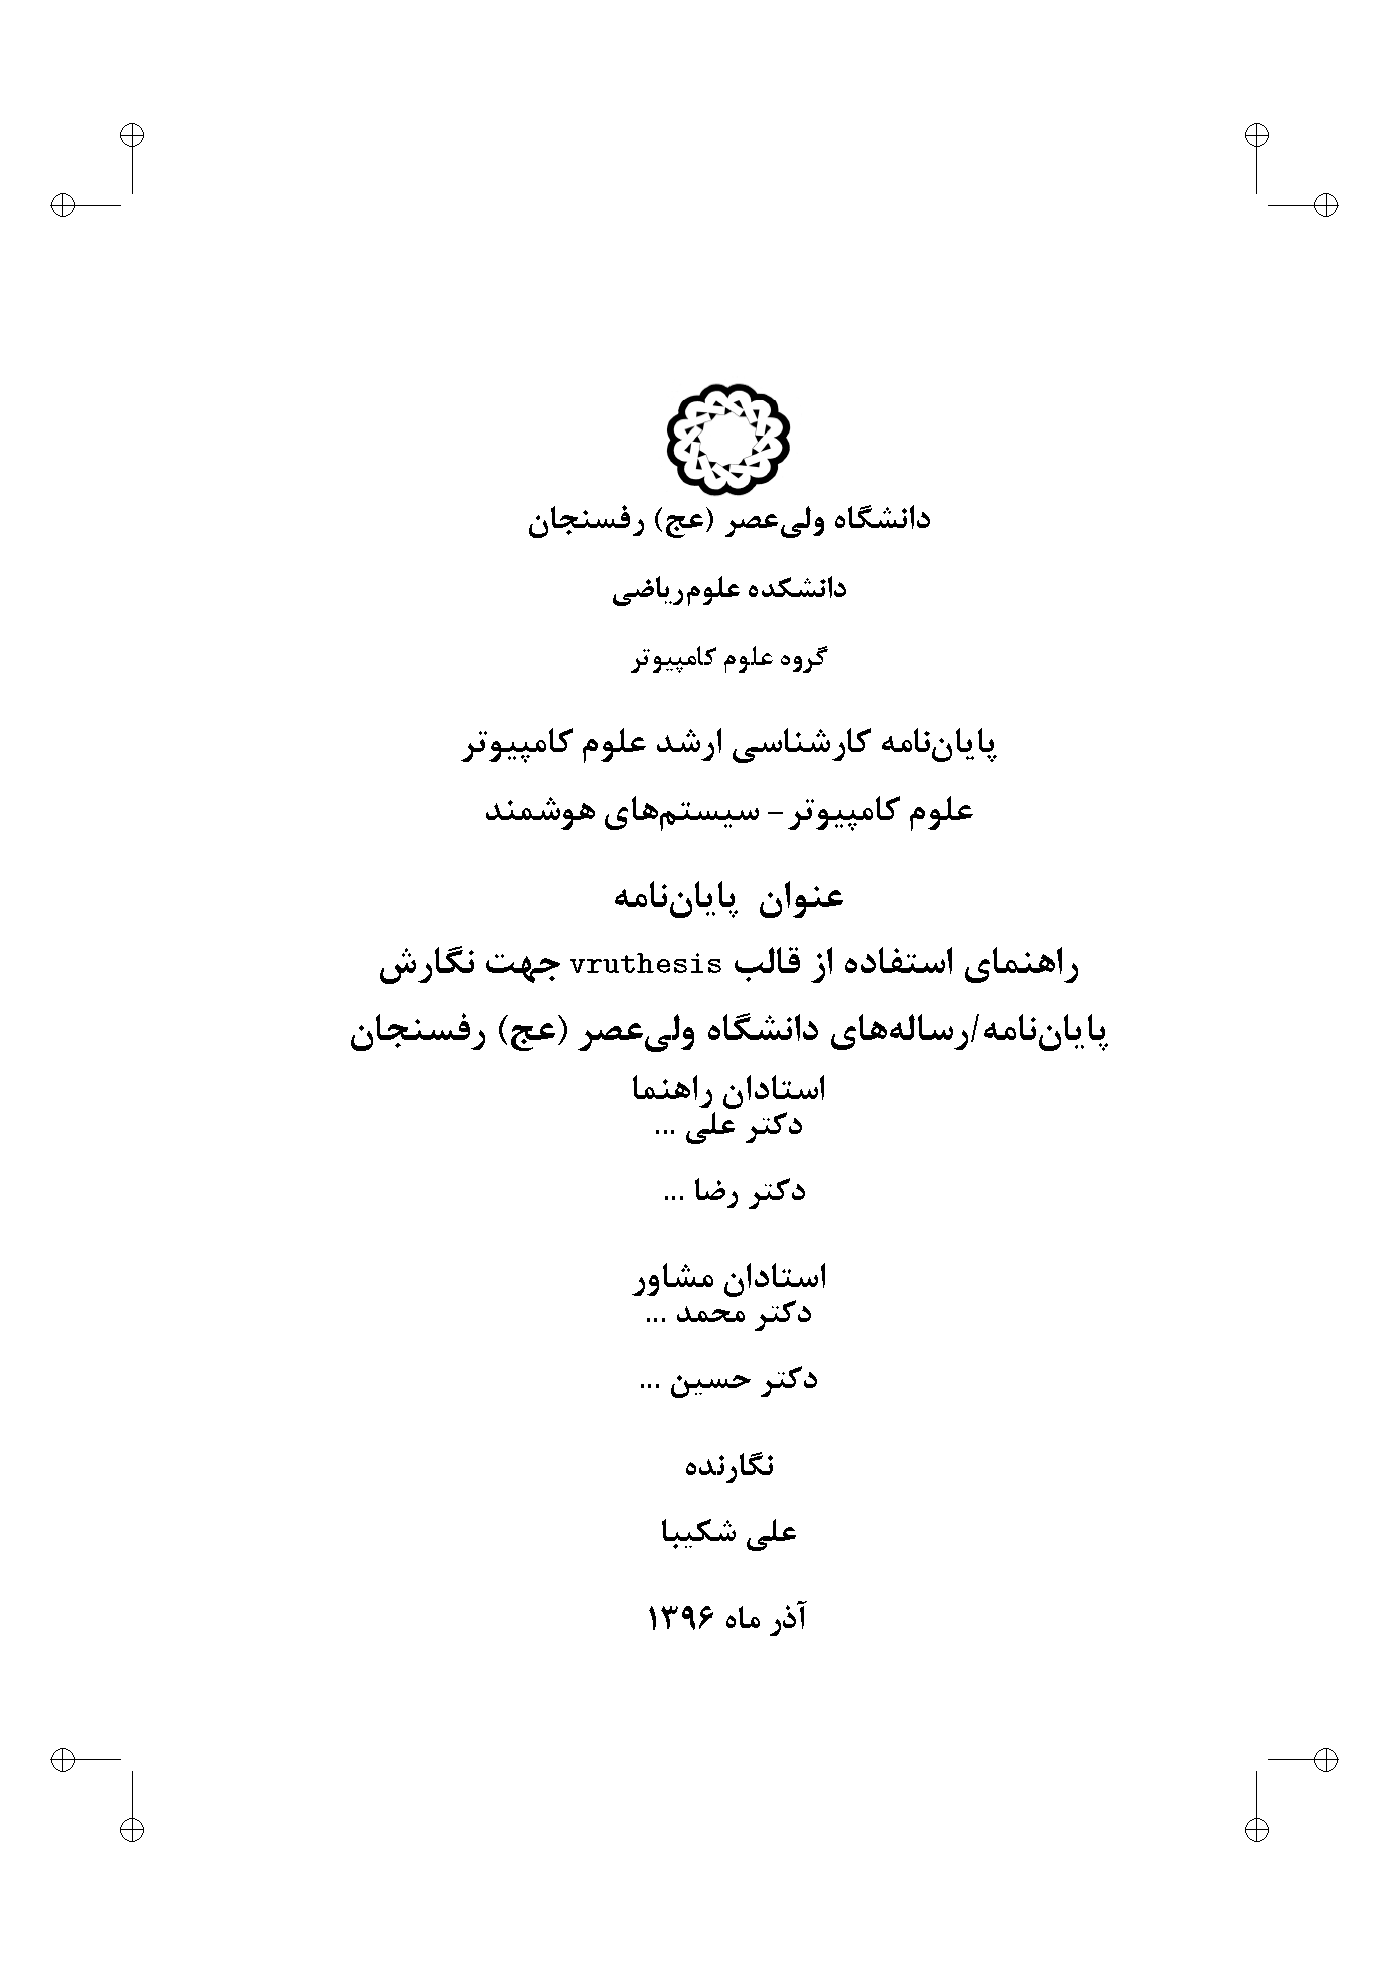
\includegraphics[width=\textwidth]{a.png}
		\caption{نمونه‌ی صفحه‌ی اول پایان‌نامه‌ی کارشناسی ارشد.}
		\label{app1}
	\end{figure}

	\begin{figure}
		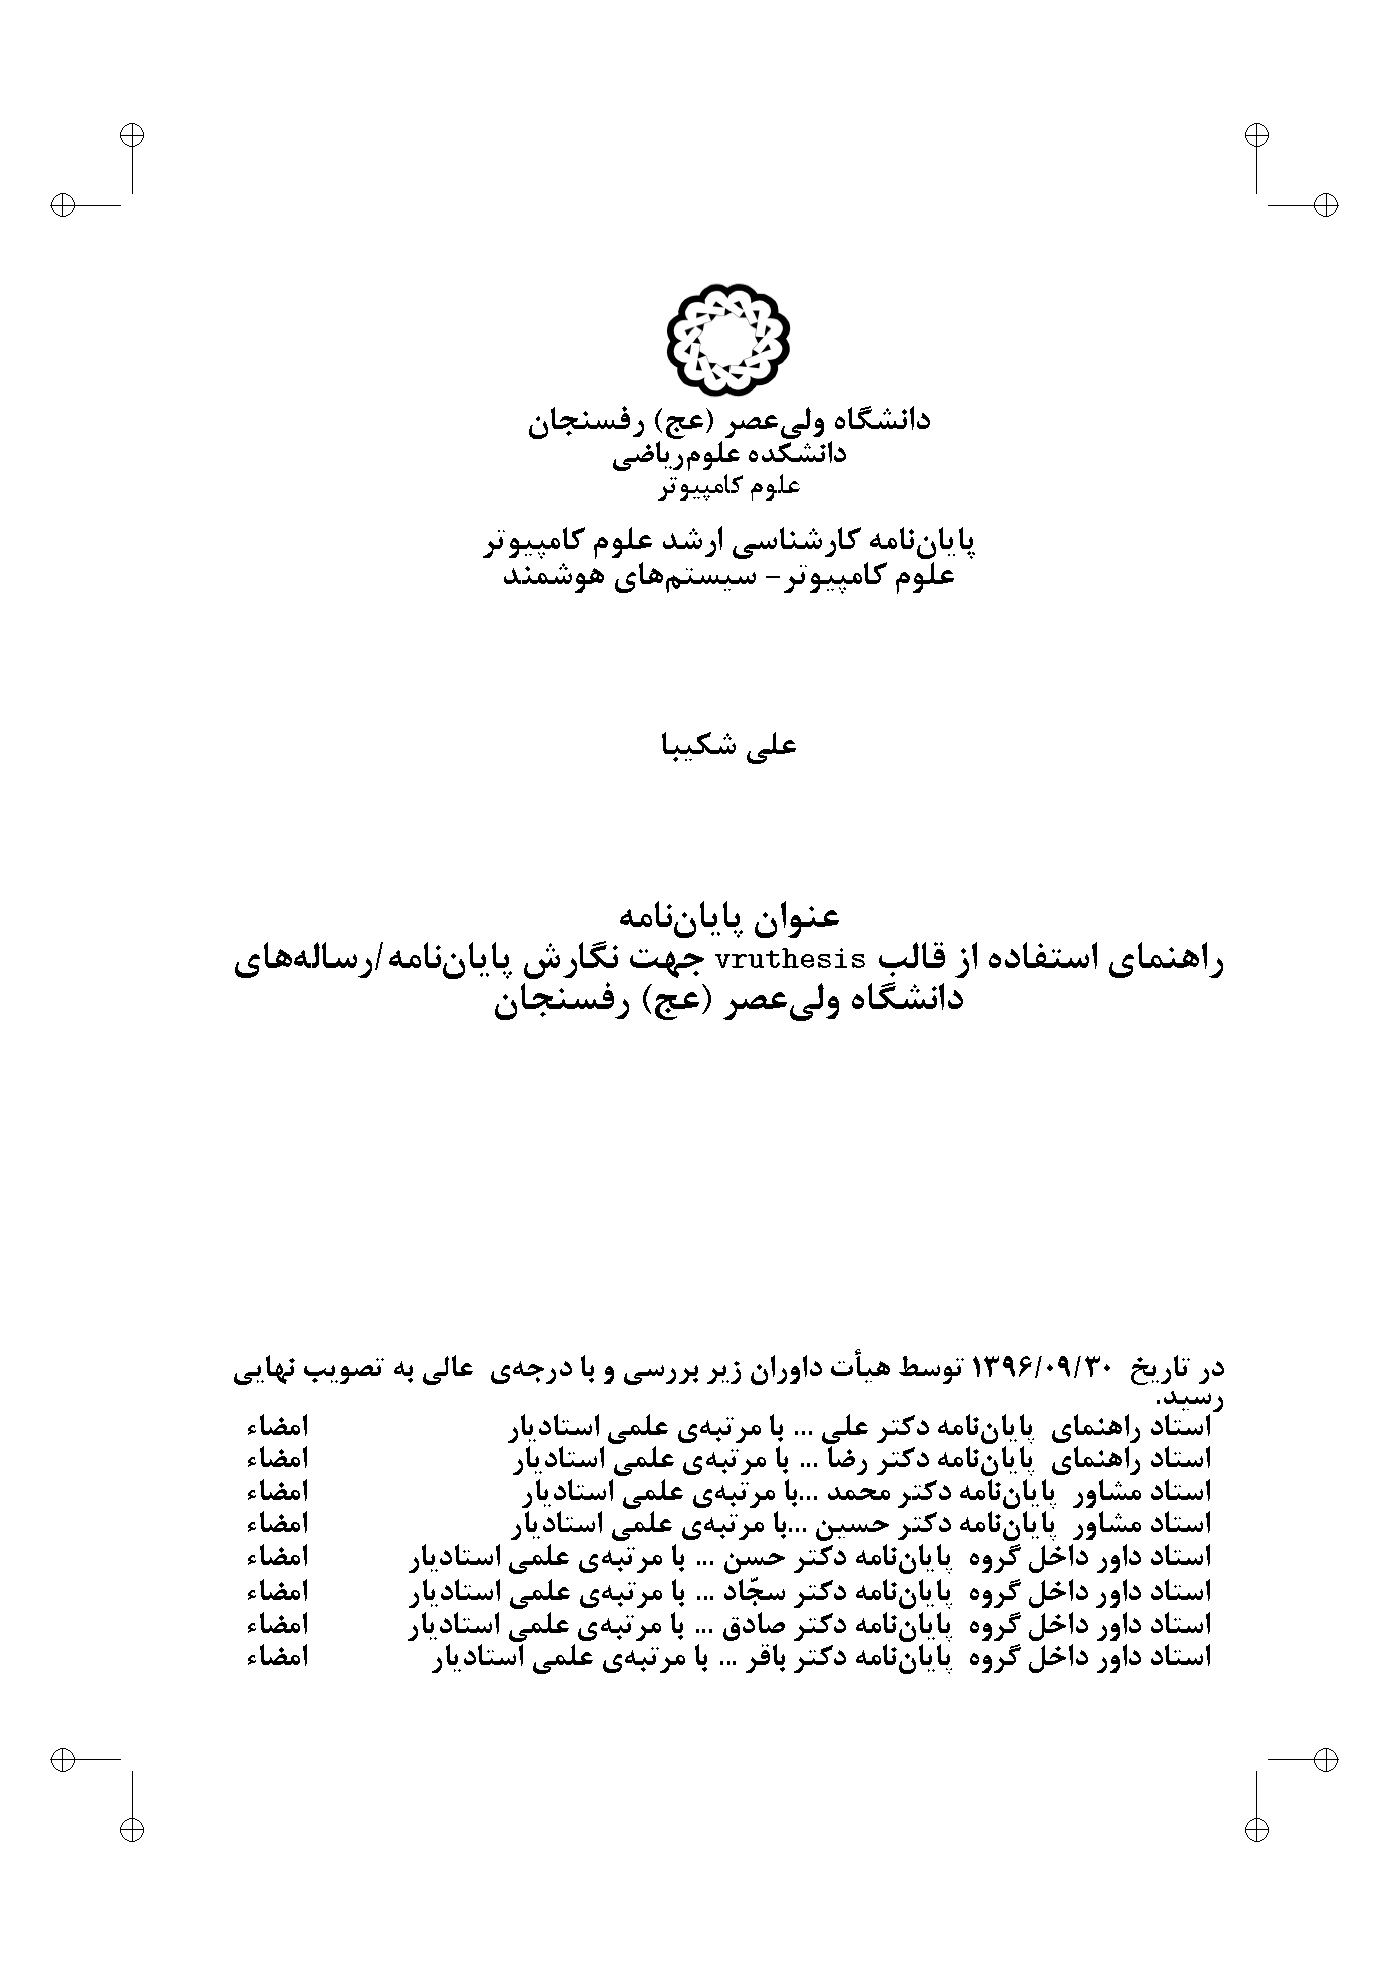
\includegraphics[width=\textwidth]{b.png}
		\caption{نمونه‌ی تصویب‌نامه‌ی پایان‌نامه‌ی کارشناسی ارشد.}
		\label{app2}
	\end{figure}

	\begin{figure}
		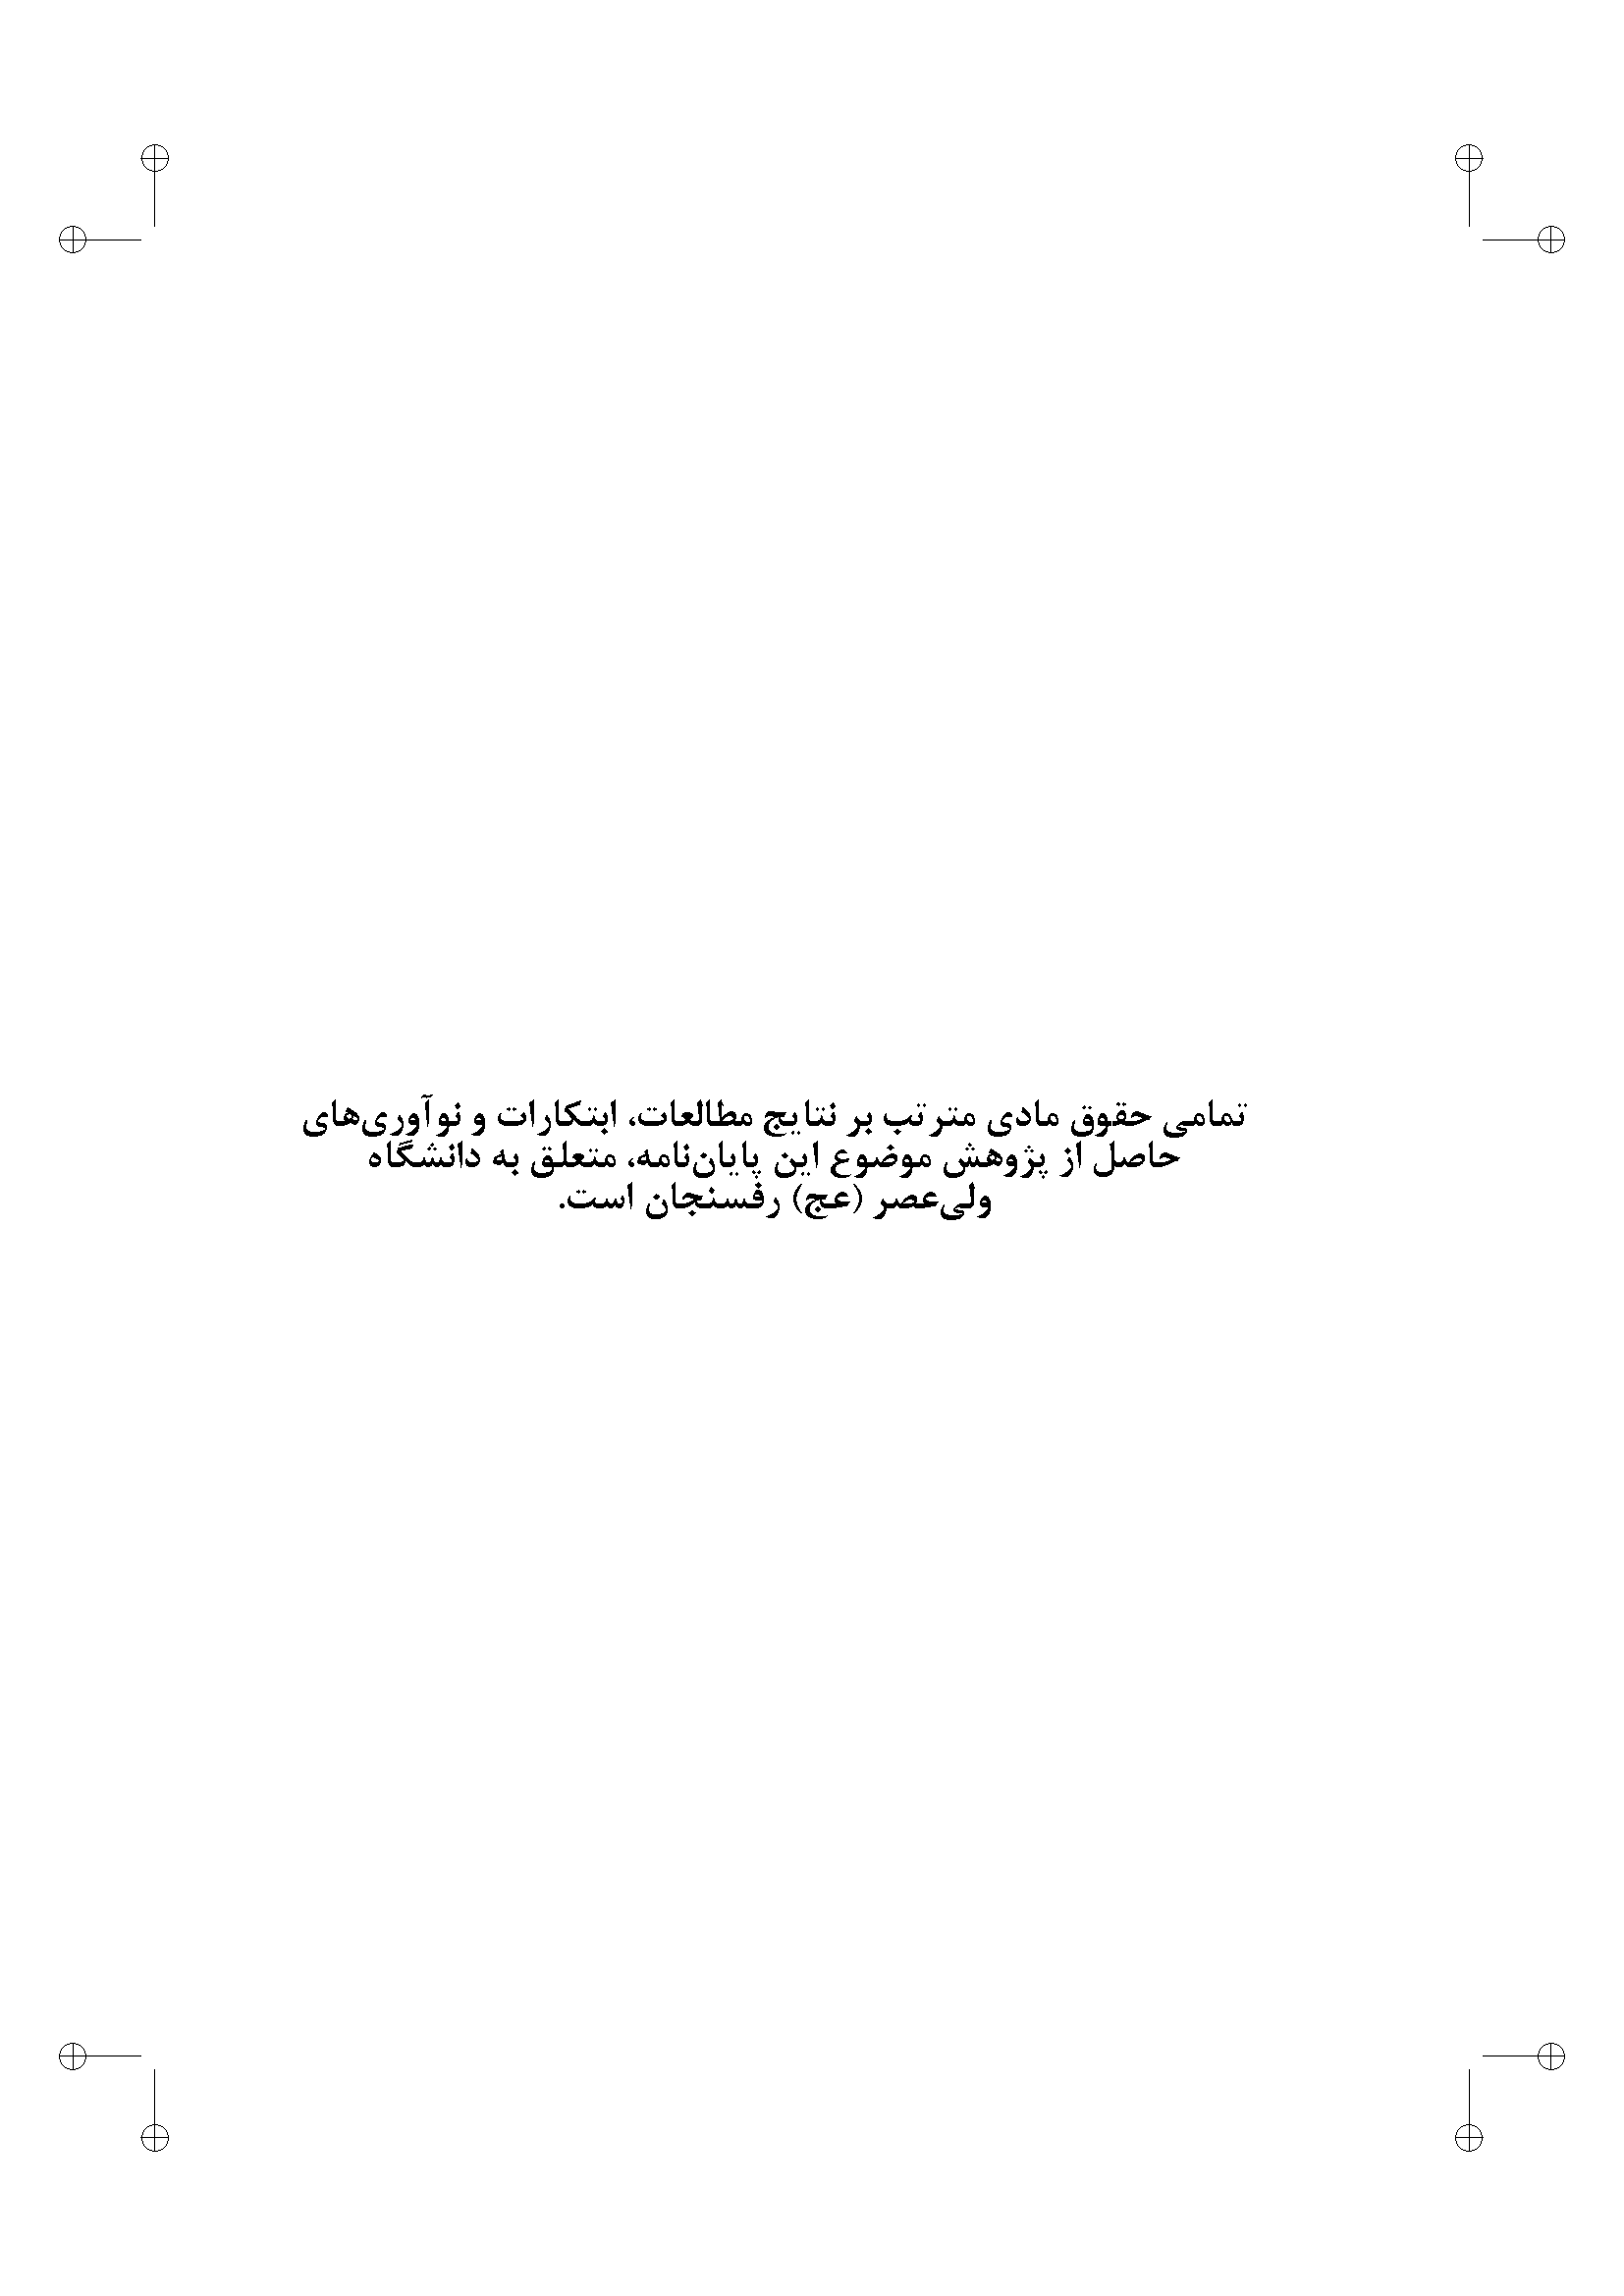
\includegraphics[width=\textwidth]{d.png}
		\caption{تعهدات حقوقی.}
		\label{app4}
	\end{figure}

	\begin{figure}
		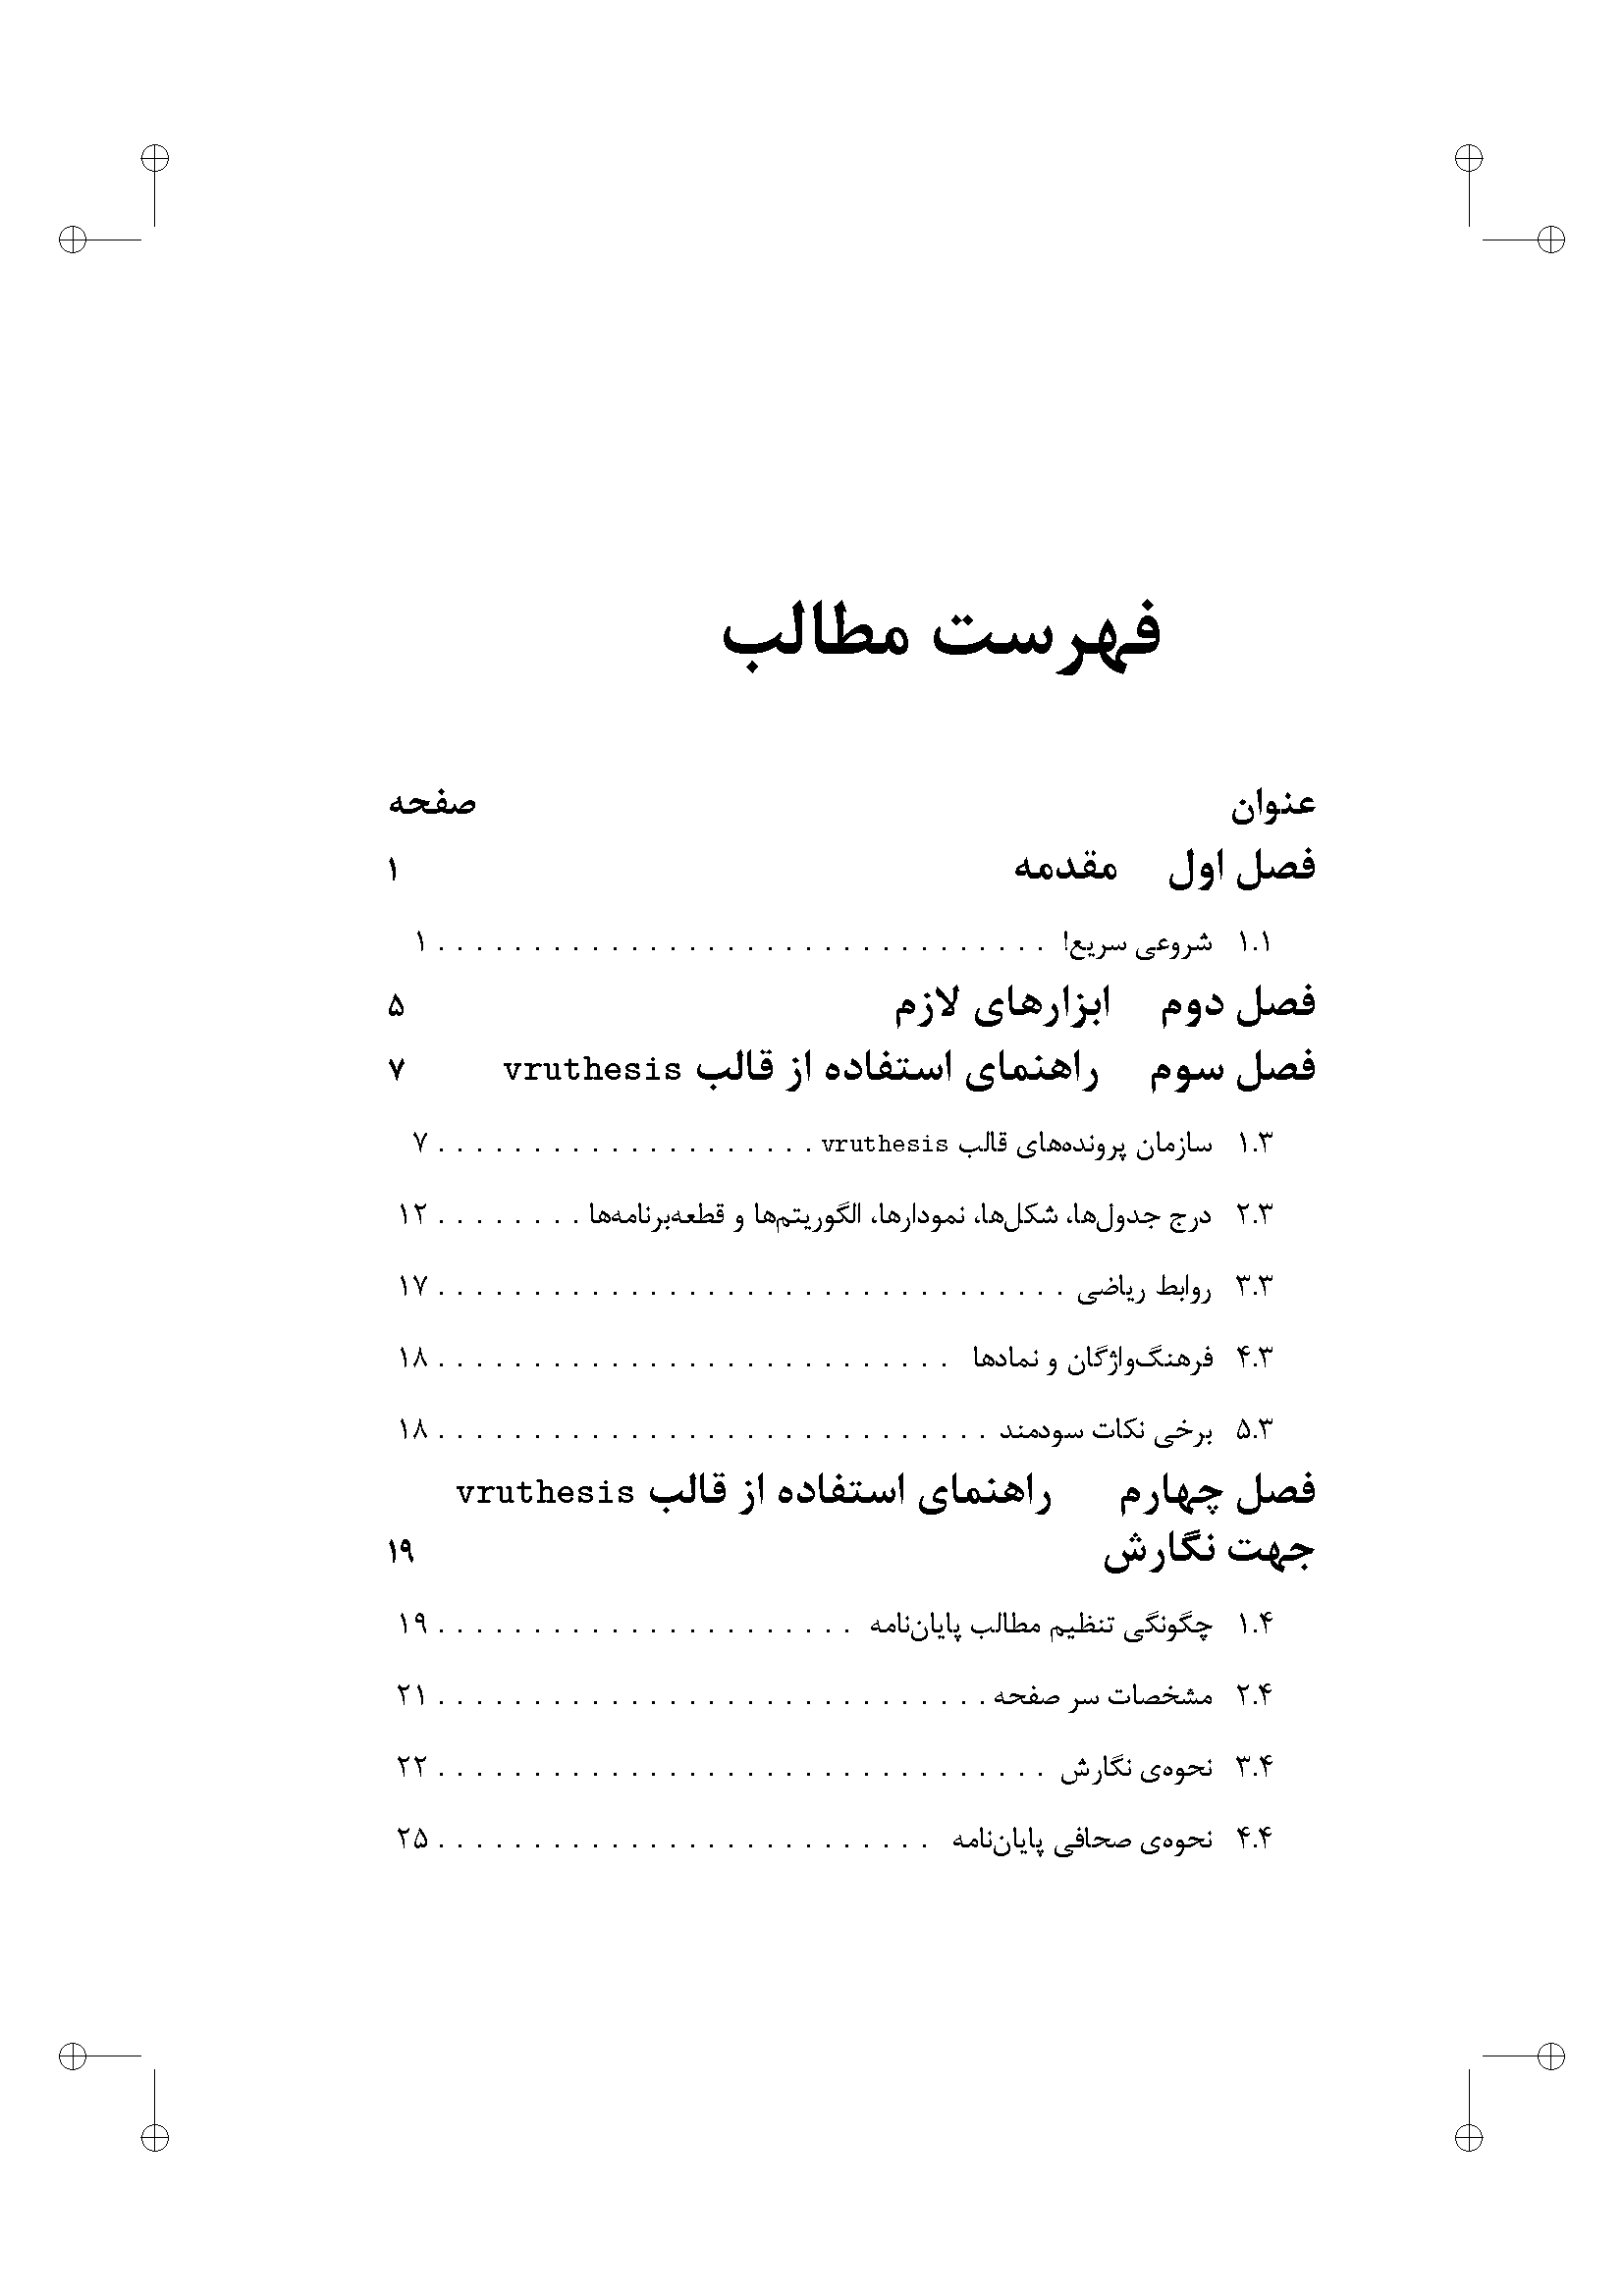
\includegraphics[width=\textwidth]{e.png}
		\caption{نمونه‌ای از فهرست مطالب.}
		\label{app5}
	\end{figure}

	\begin{figure}
		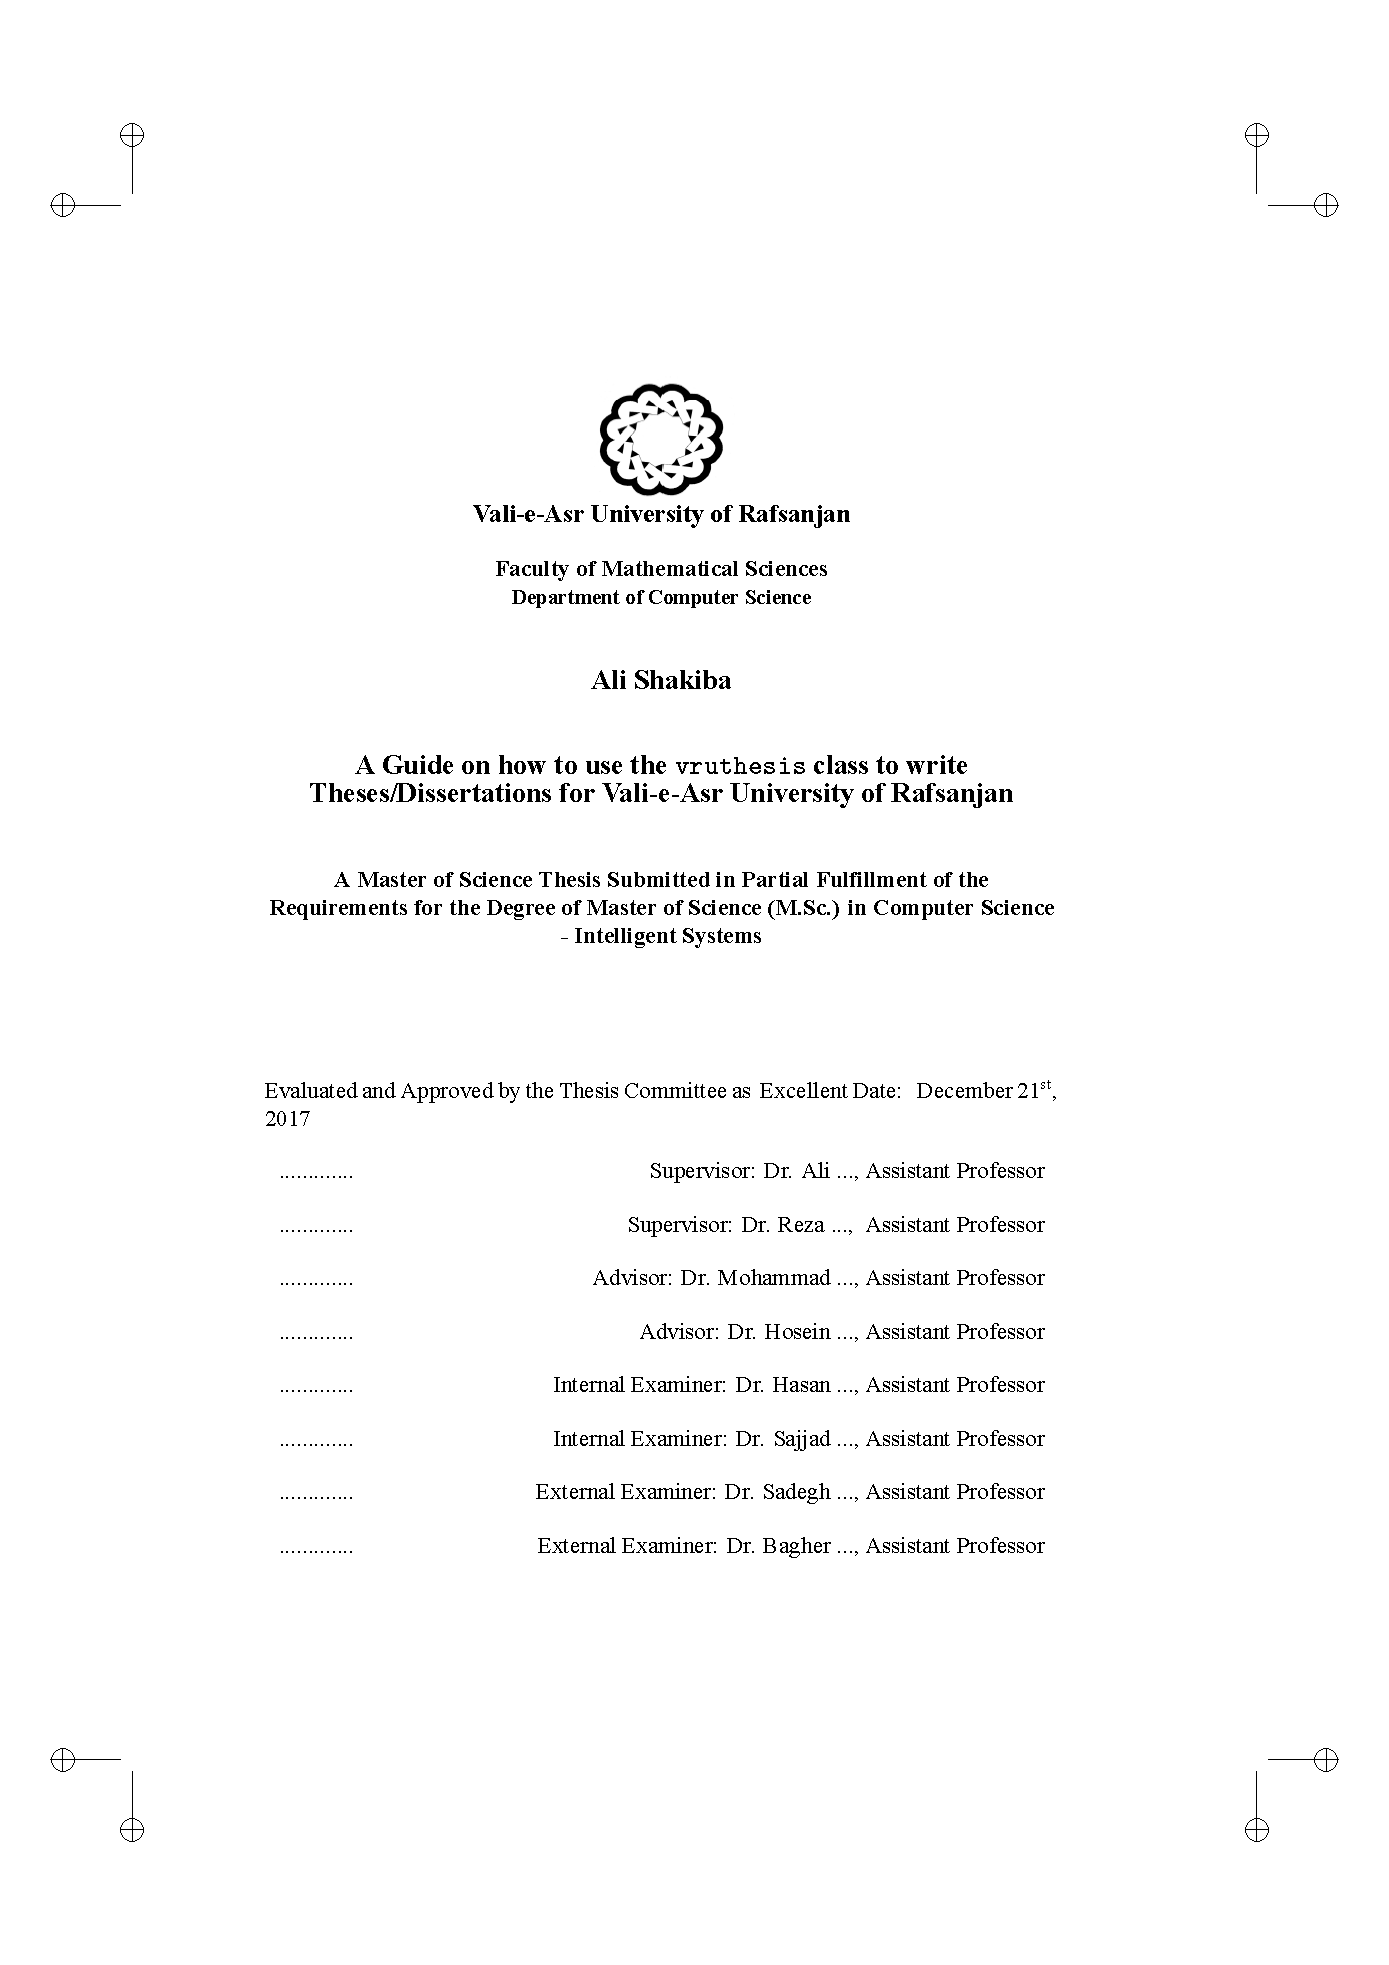
\includegraphics[width=\textwidth]{c.png}
		\caption{نمونه‌ی تصویب‌نامه‌ی پایان‌نامه‌ی کارشناسی ارشد به زبان انگلیسی.}
		\label{app3}
	\end{figure}

	\begin{figure}
		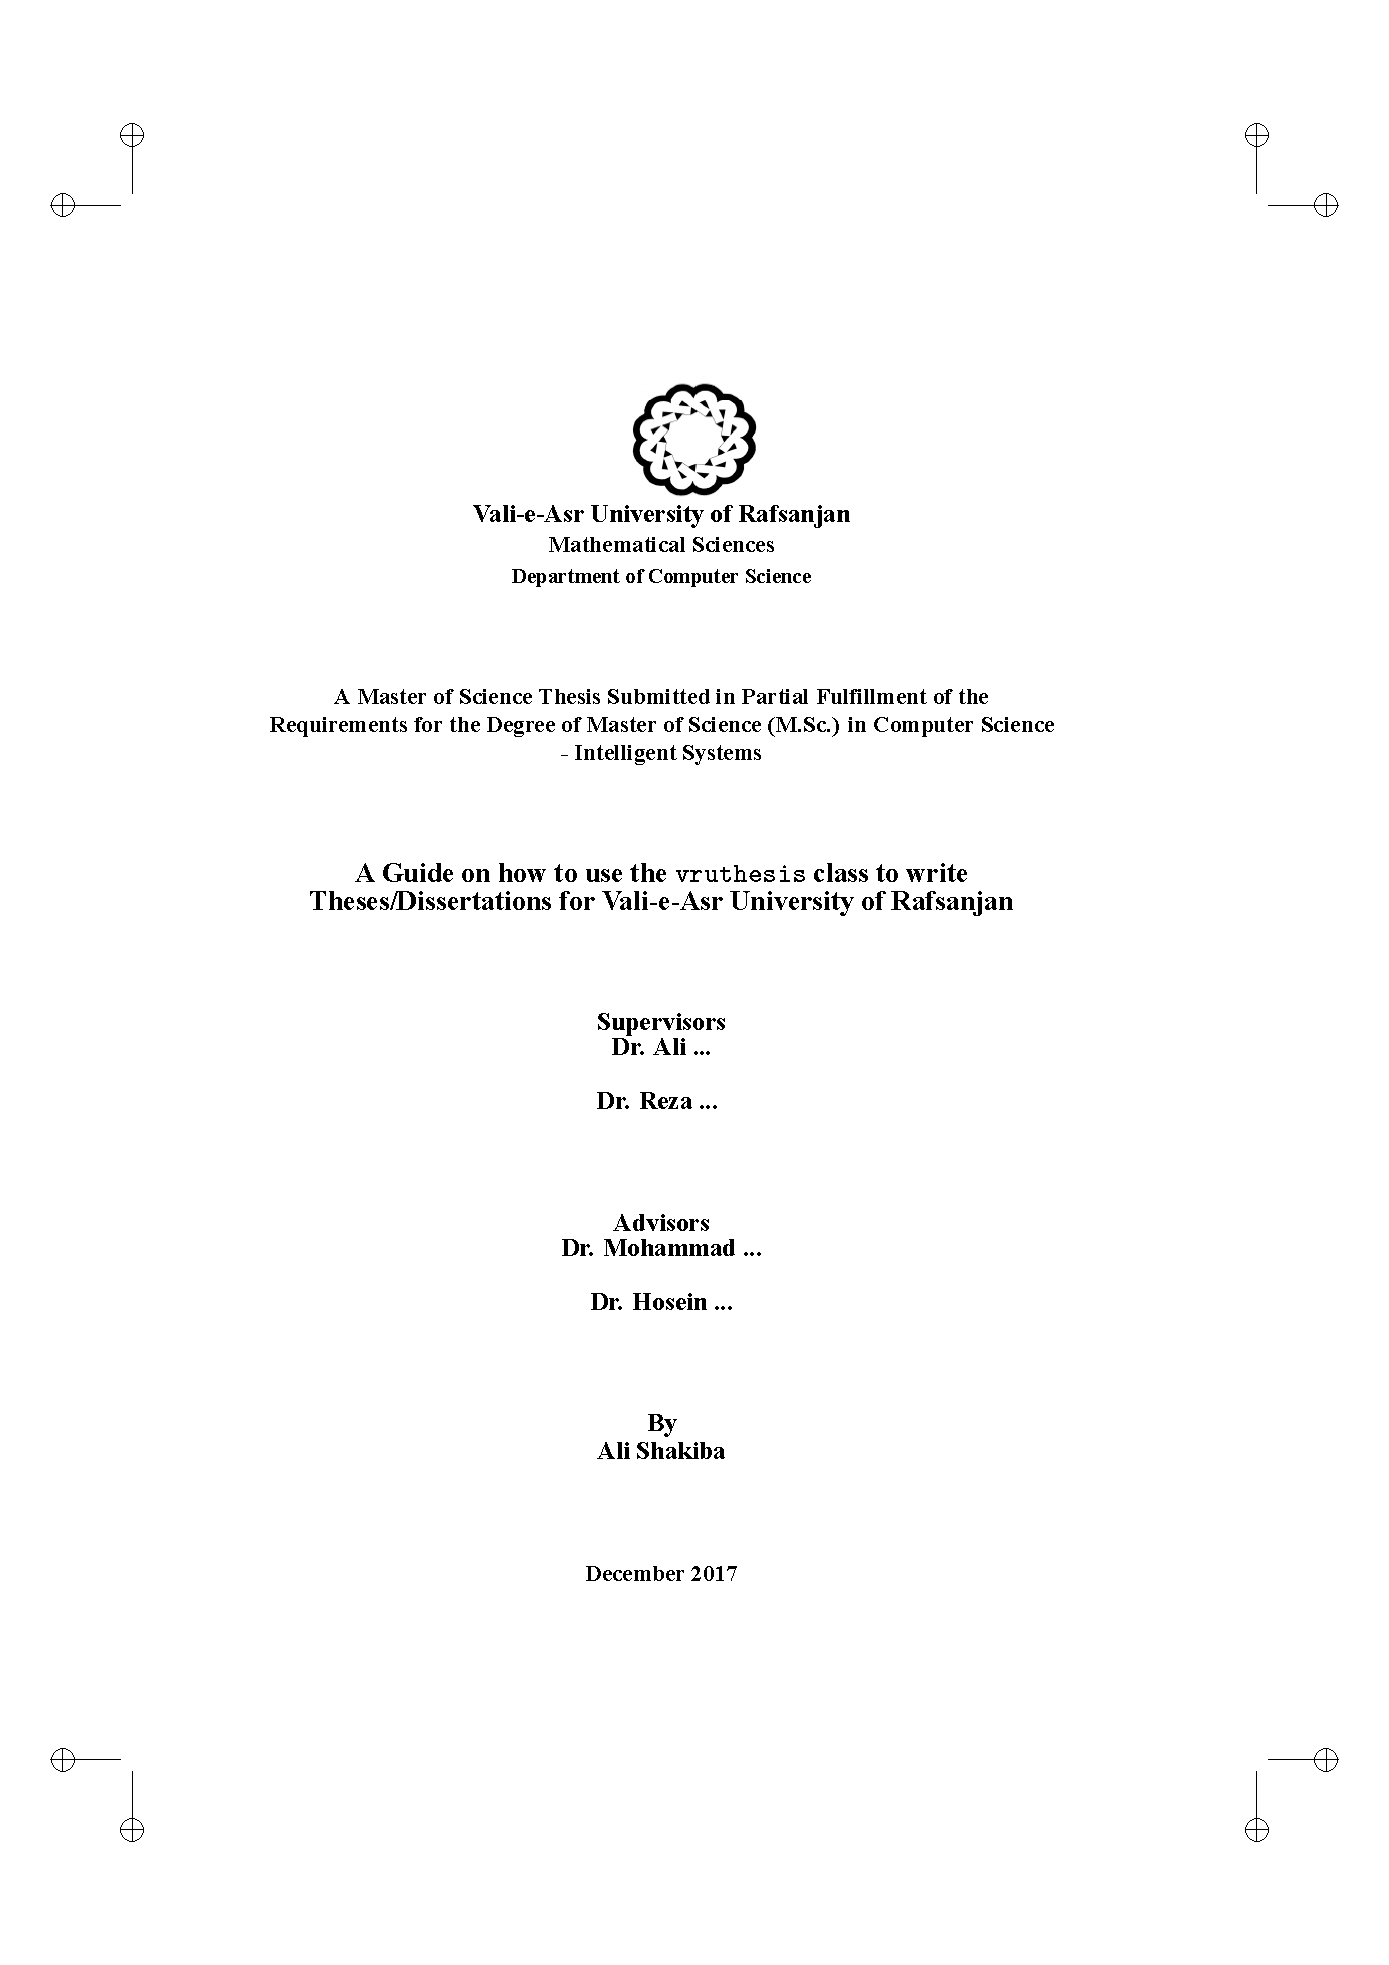
\includegraphics[width=\textwidth]{f.png}
		\caption{نمونه‌ی صفحه‌ی آخر پایان‌نامه‌ی کارشناسی ارشد.}
		\label{app6}
	\end{figure}

% +rl|از این قسمت به بعد را به هیچ وجه تغییر ندهید.$
	% لطفا هیچ تغییری در این فایل صورت ندهید.
	\cleardoublepage
	\printglossary
	\cleardoublepage
	\cleardoublepage
	\addcontentsline{toc}{chapter}{فهرست مراجع}
	\bibliography{references}
	\vrutitleen
\end{document}
		\end{mynewverbatim}
		\caption{محتویات \gls*{file} \lr{\texttt{thesis.tex}} نمونه.}
		\label{fig:ch1:thesis}
	\end{figure}
	این \gls{file} برای \gls{typeset} پایان‌نامه‌های کارشناسی ارشد دانشکده‌ی ریاضی در قطع وزیری، با چاپ دورو آماده شده است. همچنین، به منظور سهولت در فرایند صحافی، خطوط راهنما جهت برش کاغذ، در هر صفحه نمایش داده شده اند. 
	
		قواعد زیر؛ تنها قواعدی هستند که برای \gls{typeset} پایان‌نامه‌ی خود، نیاز است تا بدانید:
	\begin{itemize}
		\item اطلاعات مورد نیاز برای تولید صفحات ابتدایی و انتهایی پایان‌نامه، مانند چکیده‌، تقدیم‌به و مانند آن، در \gls{file} \lr{\texttt{data.tex}} قرار دارند. 
		\item مطالب هر یک از فصل‌ها را در یکی از \glspl{file}ی \lr{\texttt{chapterX.tex}} قرار دهید.
		\item پیوست‌ها در  \glspl{file}ی \lr{\texttt{appendixX.tex}} قرار می‌گیرند.
		\item قالب تولید فهرست مراجع در خط $10$ تعیین می‌گردد. برای تولید موفقیت آمیز فهرست مراجع، وجود \gls{file} \lr{\texttt{BibStyle.bst}} که \lr{\texttt{BibStyle}} بیانگر قالب مورد استفاده است؛ الزامی است.
		\item اطلاعات مربوط به مراجع در \gls{file} \lr{\texttt{references.bib}} به صورت \lr{bibtex} قرار می‌گیرند.
		\item واژگان در \gls{file} \lr{\texttt{gloss.tex}} و اختصارات و نمادها در \gls{file} \lr{\texttt{acronym.tex}} تعریف می‌شوند.
		\item دستورات لازم برای تولید خروجی در شکل \ref{fig:ch1:output_cmd} آمده‌اند. 
		\item وجود \glspl{file}ی \lr{\texttt{vruthesis.cls}}، \lr{\texttt{settings.tex}}، \lr{\texttt{data.tex}}، و \lr{\texttt{finalpart.tex}} جهت تولید خروجی موفق، الزامی است.
		\item در صورت نیاز برای \gls{typeset} رساله‌ی دکتری، در خط اول \gls{file} \lr{\texttt{chapterX.tex}}، کلمه‌ی \lr{phd} را به ویژگی‌ها اضافه نمایید.
		\item در صورتی که پایان‌نامه‌ی شما فاقد الگوریتم است؛ فهرست الگوریتم‌ها را با برداشتن کلمه‌ی \lr{alg} از ویژگی‌های خط اول \gls{file} \lr{\texttt{chapterX.tex}}، غیر فعال نمایید.
	\end{itemize}
				\begin{figure}
		\begin{latin}
\centering
	\begin{verbatim}
	xelatex -synctex=-1 thesis.tex
bibtex8 -W -c cp1256fa thesis
xindy -L persian-variant1 -C utf8 -I xindy -M thesis.xdy 
        -t thesis.glg -o thesis.gls thesis.glo
xindy -L persian-variant1 -C utf8 -I xindy -M thesis.xdy 
        -t thesis.blg -o thesis.bls thesis.blo
xindy -L english -C utf8 -I xindy -M thesis.xdy -t thesis.alg 
        -o thesis.acr thesis.acn
xelatex -synctex=-1 thesis.tex
xelatex -synctex=-1 thesis.tex
	\end{verbatim}
	\end{latin}
\caption{دستورات لازم برای تولید خروجی نهایی به قالب \gls*{pdf}.}
\label{fig:ch1:output_cmd}
\end{figure}
\section{یک بخش آزمایشی}
در این قسمت، نمونه‌ای از بخش‌بندی‌های ممکن نمایش داده می‌شوند.
	\subsection{یک زیربخش}
	زیربخش‌ها می‌توانند در صورت لزوم دارای زیرزیربخش باشند.
		\subsubsection{یک زیرزیربخش}
		لطفا توجه داشته باشید که بخش‌بندی بیش از چهار سطح، مجاز نیست.
\newpage
این متن جهت آزمودن تعداد خطوط در هر صفحه از ویکی‌پدیای فارسی درباره‌ی خوارزمی برداشته شده است. 
محمد بن موسی خوارزمی (زاده حدود سال ۷۸۰ میلادی و درگذشته ۸۵۰ میلادی) ریاضیدان، ستاره‌شناس، فیلسوف، جغرافیدان و مورخ شهیر ایرانی[۲] در دوره عباسیان است. وی در حدود سال ۷۸۰ میلادی (قبل از ۱۸۵ قمری)[۱] در خوارزم زاده شد. ابن ندیم و قفطی اصالت او را از خوارزم می‌دانند. لقب وی معمولاً اشاره به شهر خوارزم دارد که همان خیوه کنونی واقع در جنوب دریاچه آرال مرکزی و بخشی از جمهوری ازبکستان کنونی است.[۱] شهرت علمی وی مربوط به کارهایی است که در ریاضیات، به‌ویژه در رشته جبر، انجام داده به‌طوری‌که هیچ‌یک از ریاضیدانان سده‌های میانه مانند وی در فکر ریاضی تأثیر نداشته‌اند و وی را «پدر جبر» نامیده‌اند.[۳] جرج سارتن، مورخ مشهور علم، در طبقه‌بندی سده‌ای کتاب خود مقدمه‌ای بر تاریخ علم سده نهم میلادی را «عصر خوارزمی» می‌نامد.[۴][۵]

خوارزمی ریاضی‌دان بنام قرون وسطی است که حاصل تحقیقات و تألیفات او هنوز مورد استفاده می‌باشد و کتاب جبر و مقابله او را بسیاری از مترجمان مشهور قرون وسطی ترجمه کرده‌اند. بیشترین چیره‌دستی وی در حل معادله‌های خطی و درجه دوم بوده‌است. کتاب Algoritmi de numero Indorum که ترجمه کتاب جمع و تفریق با عددهای هندی او به لاتین است باعث شد تا دستگاه عددی در اروپا از عددنویسی رومی به عددنویسی هندی-عربی تغییر یابد؛ چیزی که هنوز نیز در اروپا و دیگر نقاط جهان فراگیر است.[۶] واژه جبر را اروپائیان بطور کلی از کتاب خوارزمی و اصطلاح امروزی الگوریتم (Algorithmus) از نام خوارزمی گرفته شده‌است. به هنگام خلافت مأمون، وی عضو دارالحکمه که مجمعی از دانشمندان در بغداد به سرپرستی مأمون بود، گردید. خوارزمی کارهای دیوفانت را در رشته جبر دنبال کرد و به بسط آن پرداخت.
گویند قبل از اینکه محمد بن موسی خوارزمی در دارالحکمه مستقر شود او را به سرزمین هند فرستادند تا حساب هندی را بیاموزد خوارزمی پس از بازگشت از هند دو اثر «حساب الهند» و دیگری «الجبر و المقابله» را نگاشت. وی نتایجی را که یونانیان و هندیان بدست آورده بودند را تلفیق کرد و بدین ترتیب سبب انتقال مجموعه‌ای از معلومات جبری حسابی شد که در ریاضیات قرون وسطی تأثیر عمیقی گذاشت.[۱۱]
محمد بن موسی خوارزمی در قرن سوم هجری، علمی را برای نخستین بار صورتبندی و تدوین کرد که خود آن را «الجبر و المقابله» نامید، علمی که تمام شرایط یک دانش واقعی را داشت، یعنی همان که اروپاییان از آن به «ساینس» تعبیر می‌کنند. این ریاضی‌دان توانست با این دانش تمام معادلات درجه دوم زمان خود راحل و راه را برای حل معادلات درجه بالاتر هموار کند.
ر اساس الواح بابلی و آثار برجای‌مانده از محاسبه‌گران هندی در عهد باستان، مردمان بابل و هند به حل حالات خاصی از معادلات درجه دوم موفق شده بودند، اما آن‌ها راه حل‌های خود را فقط به صورت دستور ارائه کردند؛ یعنی این راه حل‌ها، که برای رفع نیازهای زندگی روزمره آنان ارائه شده بودند و نه به منظور گسترش دانش ریاضی، فاقد براهین علمی بودند. ابتکار خوارزمی در آن است که وی نخست همه معادلات درجه دوم شناخته‌شده زمانش را بررسی می‌کند؛ در مرحله دوم روش حل هریک از آن‌ها را ارائه می‌دهد؛ سرانجام در مرحله سوم، این روش‌ها را با کمک علم هندسه اثبات می‌کند؛ مؤلفه‌هایی که درمجموع علم جدیدی به نام «جبر» را تشکیل می‌دهند. این علم، که از طریق ترجمه‌های لاتینی کتاب خوارزمی در قرون وسطی به اروپا راه یافت، هم در قرون وسطی و هم در عصر رنسانس تحول بزرگی در علم ریاضیات را موجب شد، چنان‌که در قرن شانزدهم میلادی نیکولو تارتالیا[واژه‌نامه ۳] و کاردان،[واژه‌نامه ۴] ریاضی‌دانان ایتالیایی که با ترجمه لاتینی جبر و مقابله، آشنا بودند روش این ریاضی‌دان ایرانی را برای حل معادله درجه سوم تعمیم دادند و بدین‌ترتیب گام دیگری در گسترش ریاضیات برداشتند.[۱۳]
خوارزمی کارهای دیوفانتوس[واژه‌نامه ۵] را در رشته جبر را دنبال کرد و به بسط آن پرداخت با توجه به این ابداع بزرگ ثابت کردند که علم نژاد و فرهنگ نمی‌شناسد و محصول ذهن انسان‌های متفکری است که در این عرصه تلاش می‌کنند.[۱۳] این علم از طریق کتاب وی «المختصر فی حساب الجبر و المقابله» در جهان اسلام شهرت یافت و ریاضیدانان بعد از خود را بشدت تحت تأثیر قرار داد که در سده ۱۲ میلادی به لاتین ترجمه شد.[۱۴]
	\chapter{ابزارهای لازم}
	برای تولید یک خروجی مناسب، نیاز به نصب و استفاده از ابزارهای زیر دارید:
	\begin{itemize}
		\item یک توزیع \lr{\LaTeX} مانند \lr{TeXLive}، \lr{MiKTeX} یا \lr{MaxTeX}. لازم به ذکر است که این قالب با استفاده از توزیع \lr{TeXLive 2017} تولید شده‌است.
		\item یک ویرایشگر متن مانند \lr{bidiTeXMaker}، \lr{TeXStudio}، \lr{TeXWorks}، \lr{Notepad++} و مانند آن‌ها. در این مورد، پیشنهاد می‌شود تا از \lr{bidiTeXMaker} یا \lr{TeXWorks} استفاده کنید.
	\end{itemize}

برای \gls{download} \gls{file} \lr{TeXLive 2017}، می‌توانید از آدرس \url{https://www.tug.org/texlive/acquire-iso.html} استفاده نمایید. در صورتی که در شبکه‌ی داخلی دانشگاه حضور دارید؛ توصیه می‌شود تا از آدرس \url{ftp://ftp.vru.ac.ir/Professor/Technical/A.shakiba/} استفاده کنید. لازم به ذکر است که \gls{file} حجیم و در حدود $4$ گیگابایت است. این راهنما بر مبنای راهنمای موجود در سایت پارسی‌لاتک\LTRfootnote{\url{http://www.parsilatex.com/wiki/\rl{راهنمای_نصب_تک‌لایو}}} نوشته شده‌ است.

به منظور یادگیری \gls{typeset} با \lr{\LaTeX} توصیه می‌شود تا از کتاب «مقدمه‌ای نه چندان کوتاه بر \lr{\LaTeX}»، ترجمه‌ی آقای مهدی امیدعلی\LTRfootnote{\url{https://www.ctan.org/tex-archive/info/lshort/persian}} استفاده نمایید. همچنین، می‌توانید در کارگاه‌های آموزشی دانشکده‌ی علوم ریاضی در ابتدای هر ترم، شرکت کنید.

\begin{figure}
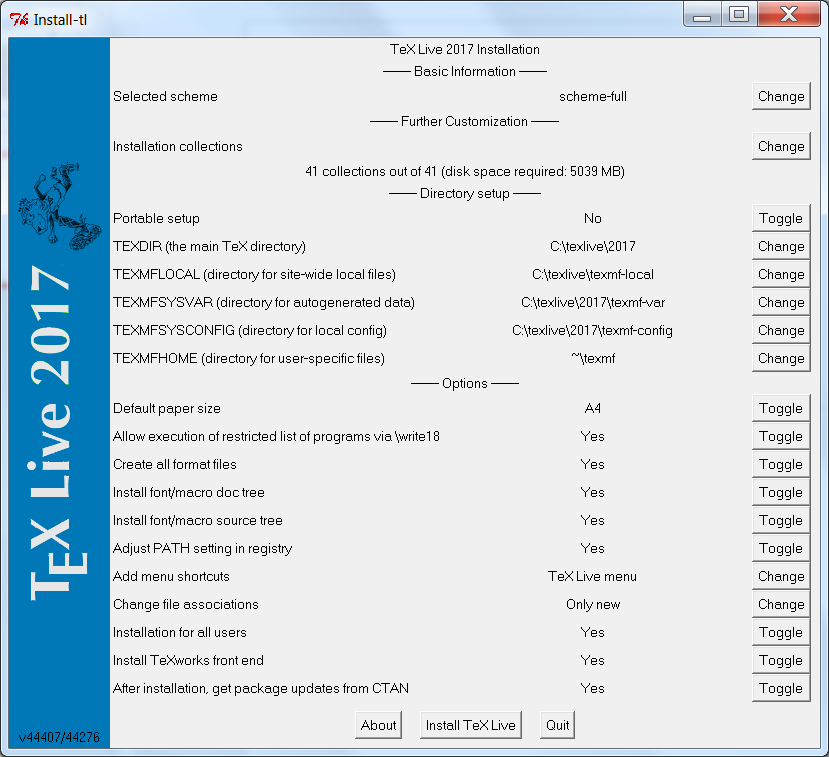
\includegraphics[width=.7\textwidth]{figs/texlive2017.png} 
\caption{پنجره‌ی نصب \lr{TeXLive 2017}.}
\end{figure}
	\chapter{راهنمای استفاده از قالب \texttt{vruthesis}}

برای \gls{typeset} پایان‌نامه‌ها و رساله‌های دانشکده‌ی علوم ریاضی، می‌توان از قالب \texttt{vruthesis} استفاده نمود. در این فصل، ابتدا در بخش \ref{sec:file_org} به سازمان \glspl{file}ی مورد استفاده در این قالب پرداخته می‌شود. شیوه‌ی قرارگیری جدول‌ها، شکل‌ها، نمودارها، الگوریتم‌ها و قطعه‌برنامه‌ها در بخش \ref{sec:figs_tbls_algs_codes} ذکر می‌شود. بخش \ref{sec:eqs} به \gls{typeset}ِ روابط ریاضی اختصاص دارد. نکات مربوط به فرهنگ‌واژگان و نمادها در بخش \ref{sec:gloss} ذکر شده‌اند. در پایان، بخش \ref{sec:faq}، برخی از نکات سودمند در استفاده از این قالب را گوشزد می‌کند.

\section{سازمان \glspl*{file}ی قالب \texttt{vruthesis}}\label{sec:file_org} 
	متن یک پایان‌نامه به طور معمول، یک متن طولانی است. بنابراین، بهتر است تنظیمات \gls{formatting} و محتوای پایان‌نامه را از یکدیگر جدا کنیم. تنظیمات \gls{formatting} در \gls{file} \texttt{vruthesis.cls} آمده است. علاوه بر این، به منظور مدیریت بهتر بر محتوا، محتوای پایان‌نامه نیز بر اساس فصل در \glspl{file}ی متعدد، تقسیم‌بندی شده‌اند. به منظور سادگی بیشتر، نمونه‌ی یک پایان‌نامه‌ی کارشناسی ارشد و نمونه‌ی یک رساله‌ی دکتر در \gls{site} دانشکده قرار گرفته‌اند. هر یک از این نمونه‌ها، شامل چند \gls{file} مختلف هستند. فهرست این \glspl{file} و کاربرد هر یک از آن‌ها در جدول \ref{tbl:fileList} آمده است. استفاده از دستوراتی که در شرح آن‌ها، عبارت «در صورت وجود» آمده است؛ اختیاری است و در صورتی که این دستورات در \gls{file} \verb|data.tex| نیامده باشند یا به صورت توضیح درج شده باشند؛ خروجی به صورت متناسب تولید می‌گردد.

\begin{table}[ht]
	\caption[\glspl*{file}ی موجود در نمونه‌ی پایان‌نامه دانشکده.]{فهرست و کاربرد \glspl*{file}ی موجود در نمونه‌ی پایان‌نامه‌ی دانشکده‌ی علوم ریاضی.}
	\label{tbl:fileList}
	\centering
	\begin{tabular}{| R{0.60\textwidth} | L{0.25\textwidth} |}
		\hline 
		\textbf{شرح} & \textbf{نام \gls{file}} \\
		\hline
		\glspl{file} اصلی پایان‌نامه، شامل ارجاع به تنظیمات، محتوا و سایر دستورات & \texttt{thesis.tex} \\ \hline
		قالب \texttt{vruthesis} & \texttt{vruthesis.cls} \\ \hline
		اطلاعات مربوط به صفحات ابتدایی و انتهایی پایان‌نامه مانند عنوان (لاتین)، چکیده (لاتین) و مانند آن & \texttt{data.tex} \\ \hline
		تعریف منابع و مآخذ به صورت \texttt{bibtex} &  \texttt{references.bib} \\ \hline
		\gls{formatting} مراجع مطابق با استاندارد \lr{IEEE} با تغییرات مصوب گروه علوم‌کامپیوتر &  \texttt{ieeetr-fa-vru.bst} \\ \hline
		\gls{formatting} مراجع مطابق با استاندارد \lr{ACM} با در نظر گرفتن مراجع فارسی &  \texttt{acm-fa.bst} \\ \hline
		محتویات مربوط به فصل \lr{X} پایان‌نامه &  \texttt{chapterX.tex} \\ \hline
		محتویات مربوط به پیوست \lr{X} پایان‌نامه &  \texttt{appendixX.tex} \\ \hline
		اطلاعات مورد نیاز برای ساخت فهرست واژگان & \texttt{gloss.tex} \\ \hline
		فهرست اختصارات و نمادها & \texttt{acronym.tex} \\ \hline
	\end{tabular}
\end{table}

	برای تولید \gls{file} نهایی پایان‌نامه در قالب \gls{pdf}، لازم است تا از موتور \lr{TeX Live 2017} استفاده شود. دستورات مورد نیاز برای تولید خروجی، در شکل \ref{fig:output_cmd} ذکر شده‌اند. 
	
	\begin{figure}
		\begin{latin}
\centering
	\begin{verbatim}
	xelatex -synctex=-1 thesis.tex
bibtex8 -W -c cp1256fa thesis
xindy -L persian-variant1 -C utf8 -I xindy -M thesis.xdy 
        -t thesis.glg -o thesis.gls thesis.glo
xindy -L persian-variant1 -C utf8 -I xindy -M thesis.xdy 
        -t thesis.blg -o thesis.bls thesis.blo
xindy -L english -C utf8 -I xindy -M thesis.xdy -t thesis.alg 
        -o thesis.acr thesis.acn
xelatex -synctex=-1 thesis.tex
xelatex -synctex=-1 thesis.tex
	\end{verbatim}
	\end{latin}
\caption{دستورات لازم برای تولید خروجی نهایی به قالب \gls*{pdf}.}
\label{fig:output_cmd}
\end{figure}

در پایان‌نامه‌ی نمونه، $5$ فصل و یک پیوست درنظر گرفته شده است. در صورتی که در پایان‌نامه‌ی خود، به فصل‌های (پیوست‌های) بیشتری نیاز دارید؛ می‌توانید با تهیه‌ی یک رونوشت از \gls{file} \texttt{chapterX.tex} (\texttt{appendixX.tex}) و ذخیره‌ی آن به نام دلخواه، فصل (پیوست) جدیدی را ایجاد کنید. لازم به ذکر است که برای لحاظ شدن فصل جدید در خروجی، نیاز است تا در \gls{file} \texttt{thesis.tex}، دستور
\begin{latin}
	\begin{verbatim}
	\include{chapterX}
	\end{verbatim}
\end{latin}
را پس از {\verb|\chapter{نتیجه‌گیری}
در این فصل، نتیجه‌گیری پایان‌نامه‌ی خود را درج کنید.
			|} یا آخرین فصل اضافه شده، قرار دهید. به طور مشابه، برای لحاظ شدن پیوست جدید در خروجی، لازم است تا دستور \verb|\include{appendixX}| پس از \verb|\chapter{یک پیوست}
مطالب این پیوست بر اساس راهنمای نگارش پایان‌نامه‌های تحصیلات تکمیلی در \cite{vru_grad_rules} تهیه شده‌اند. 

	\begin{figure}
		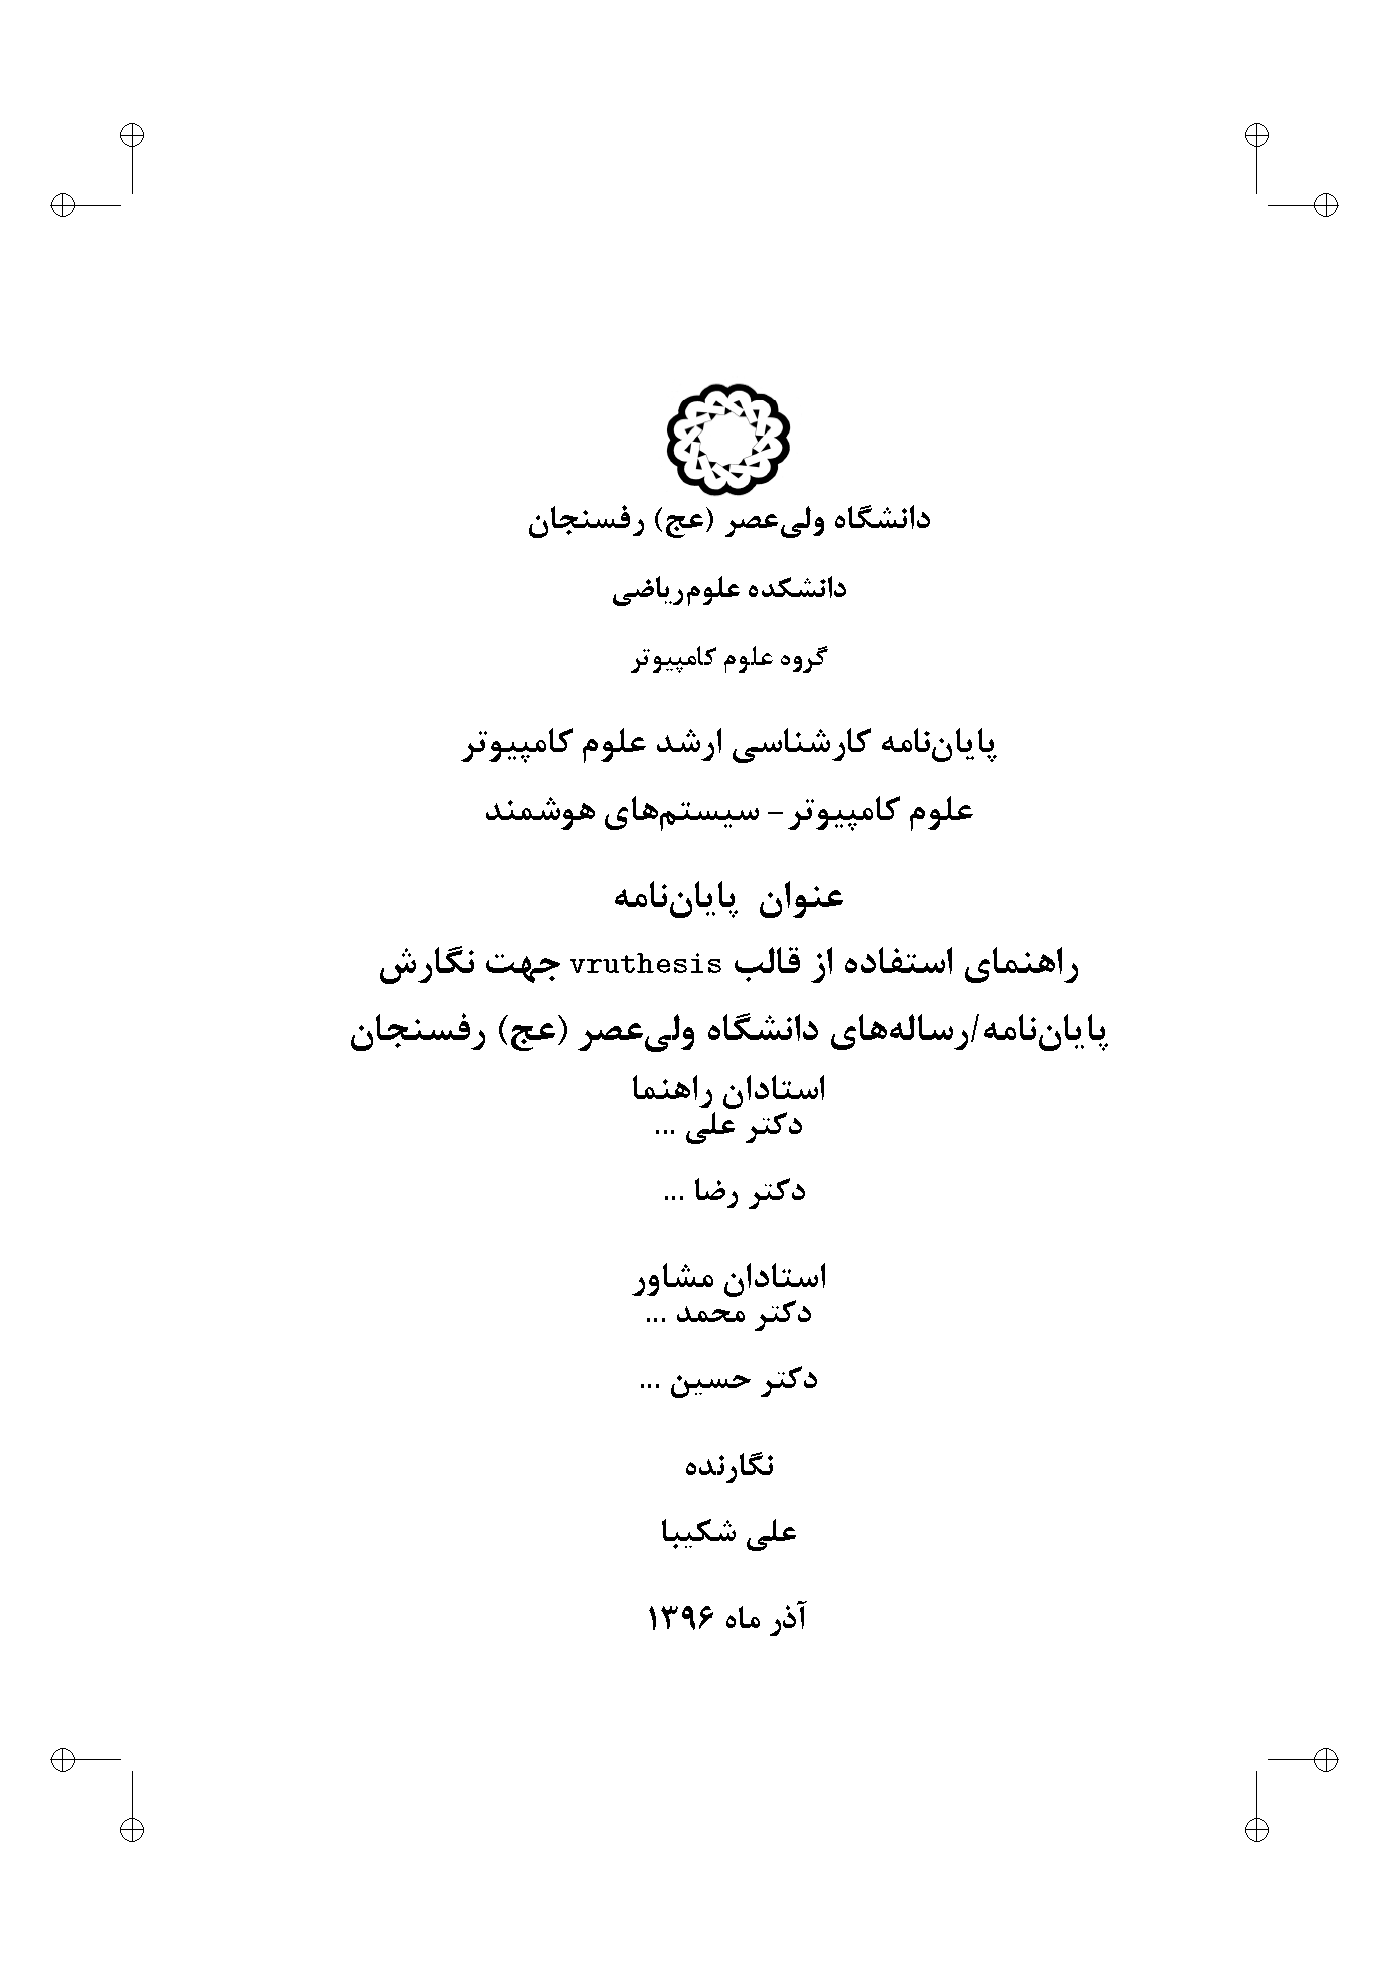
\includegraphics[width=\textwidth]{a.png}
		\caption{نمونه‌ی صفحه‌ی اول پایان‌نامه‌ی کارشناسی ارشد.}
		\label{app1}
	\end{figure}

	\begin{figure}
		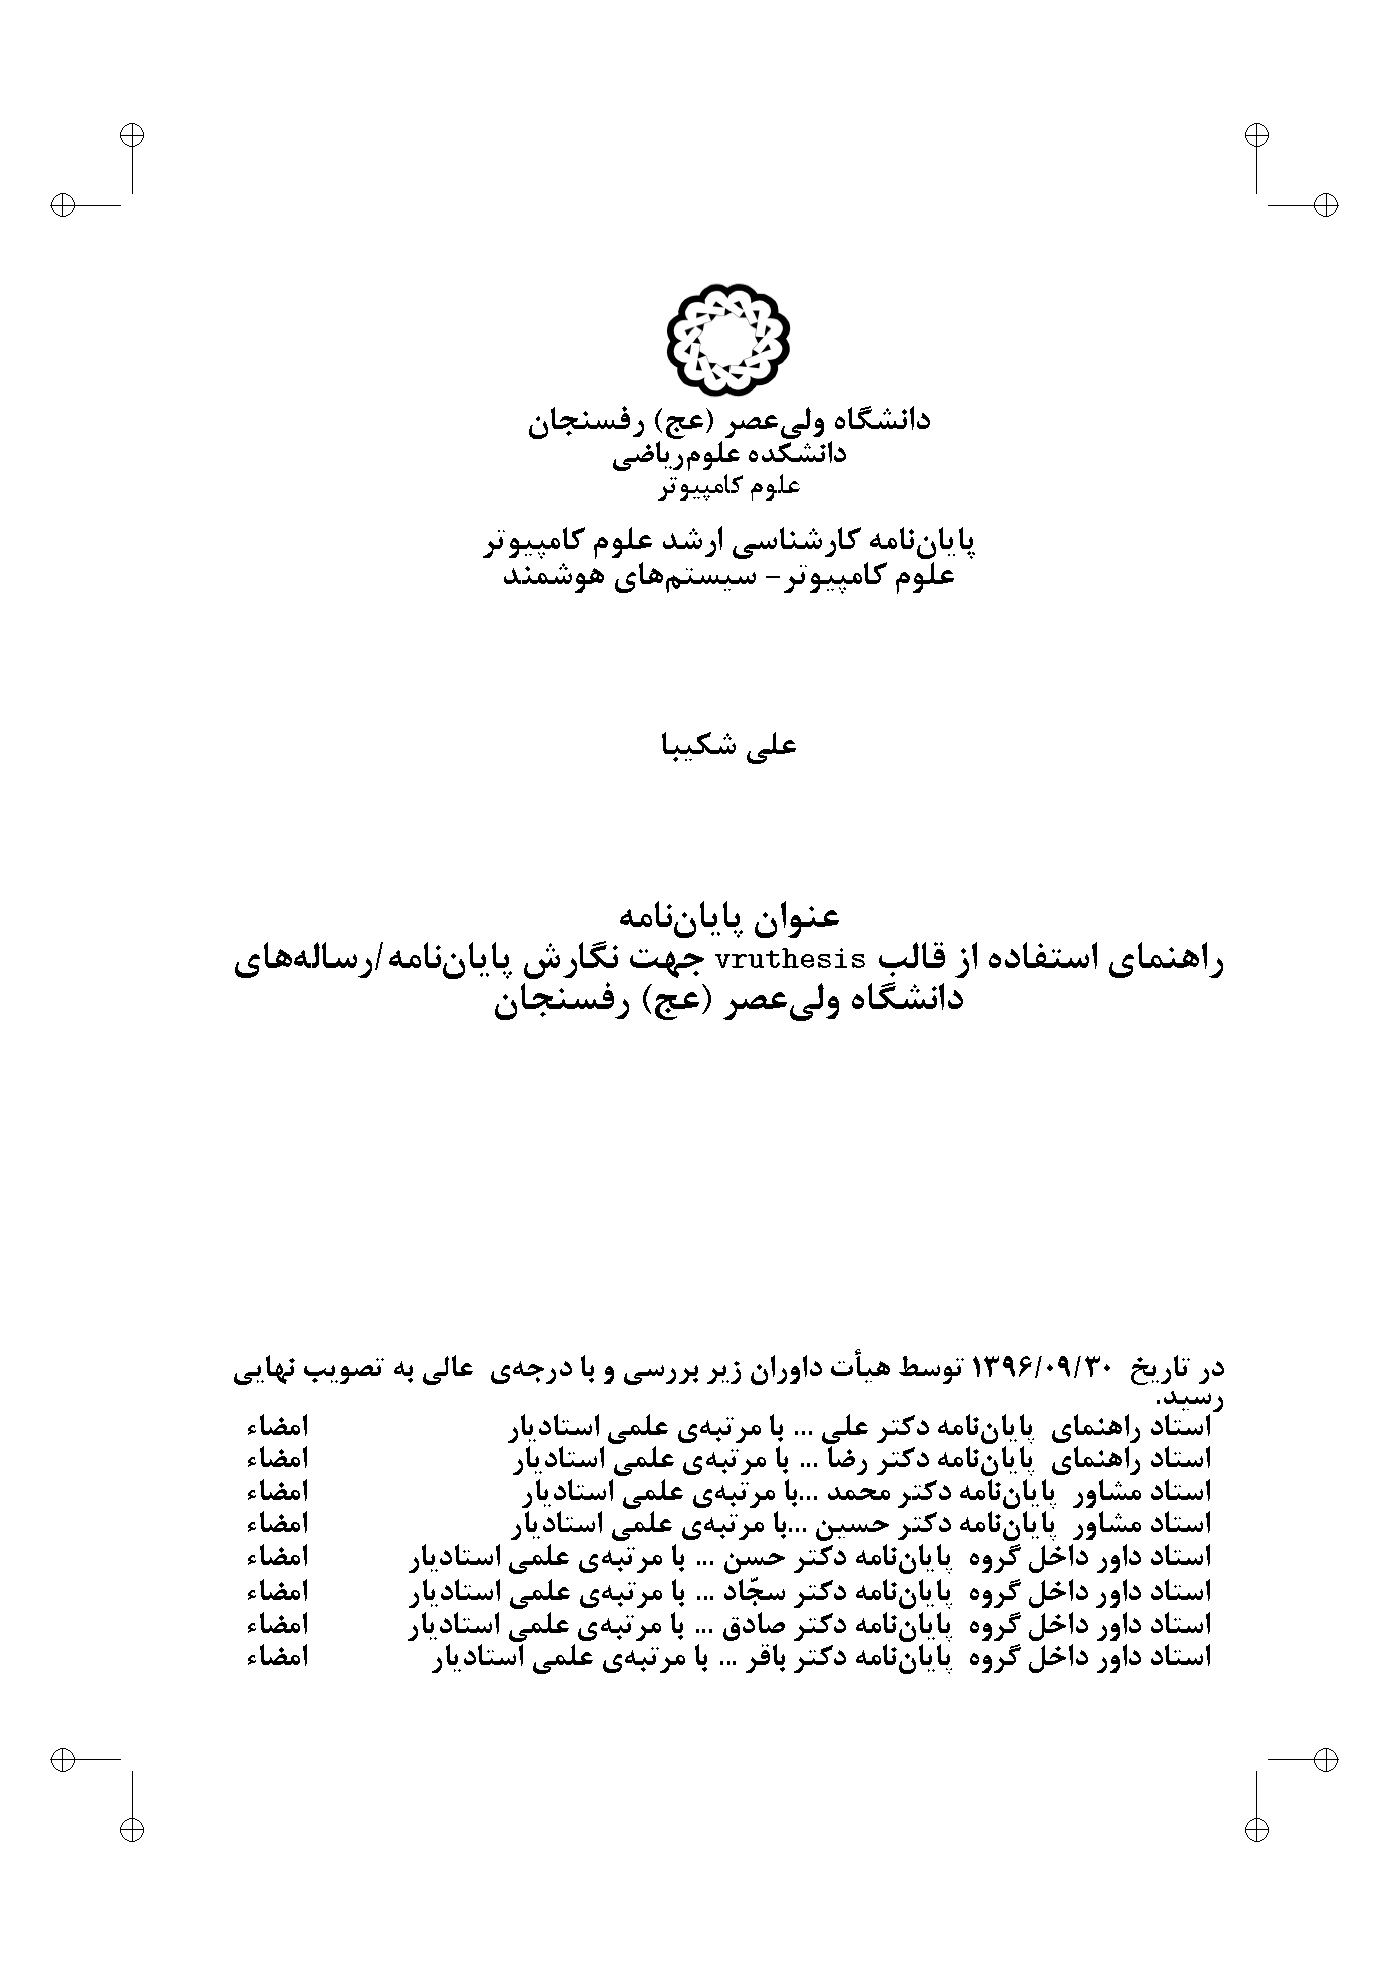
\includegraphics[width=\textwidth]{b.png}
		\caption{نمونه‌ی تصویب‌نامه‌ی پایان‌نامه‌ی کارشناسی ارشد.}
		\label{app2}
	\end{figure}

	\begin{figure}
		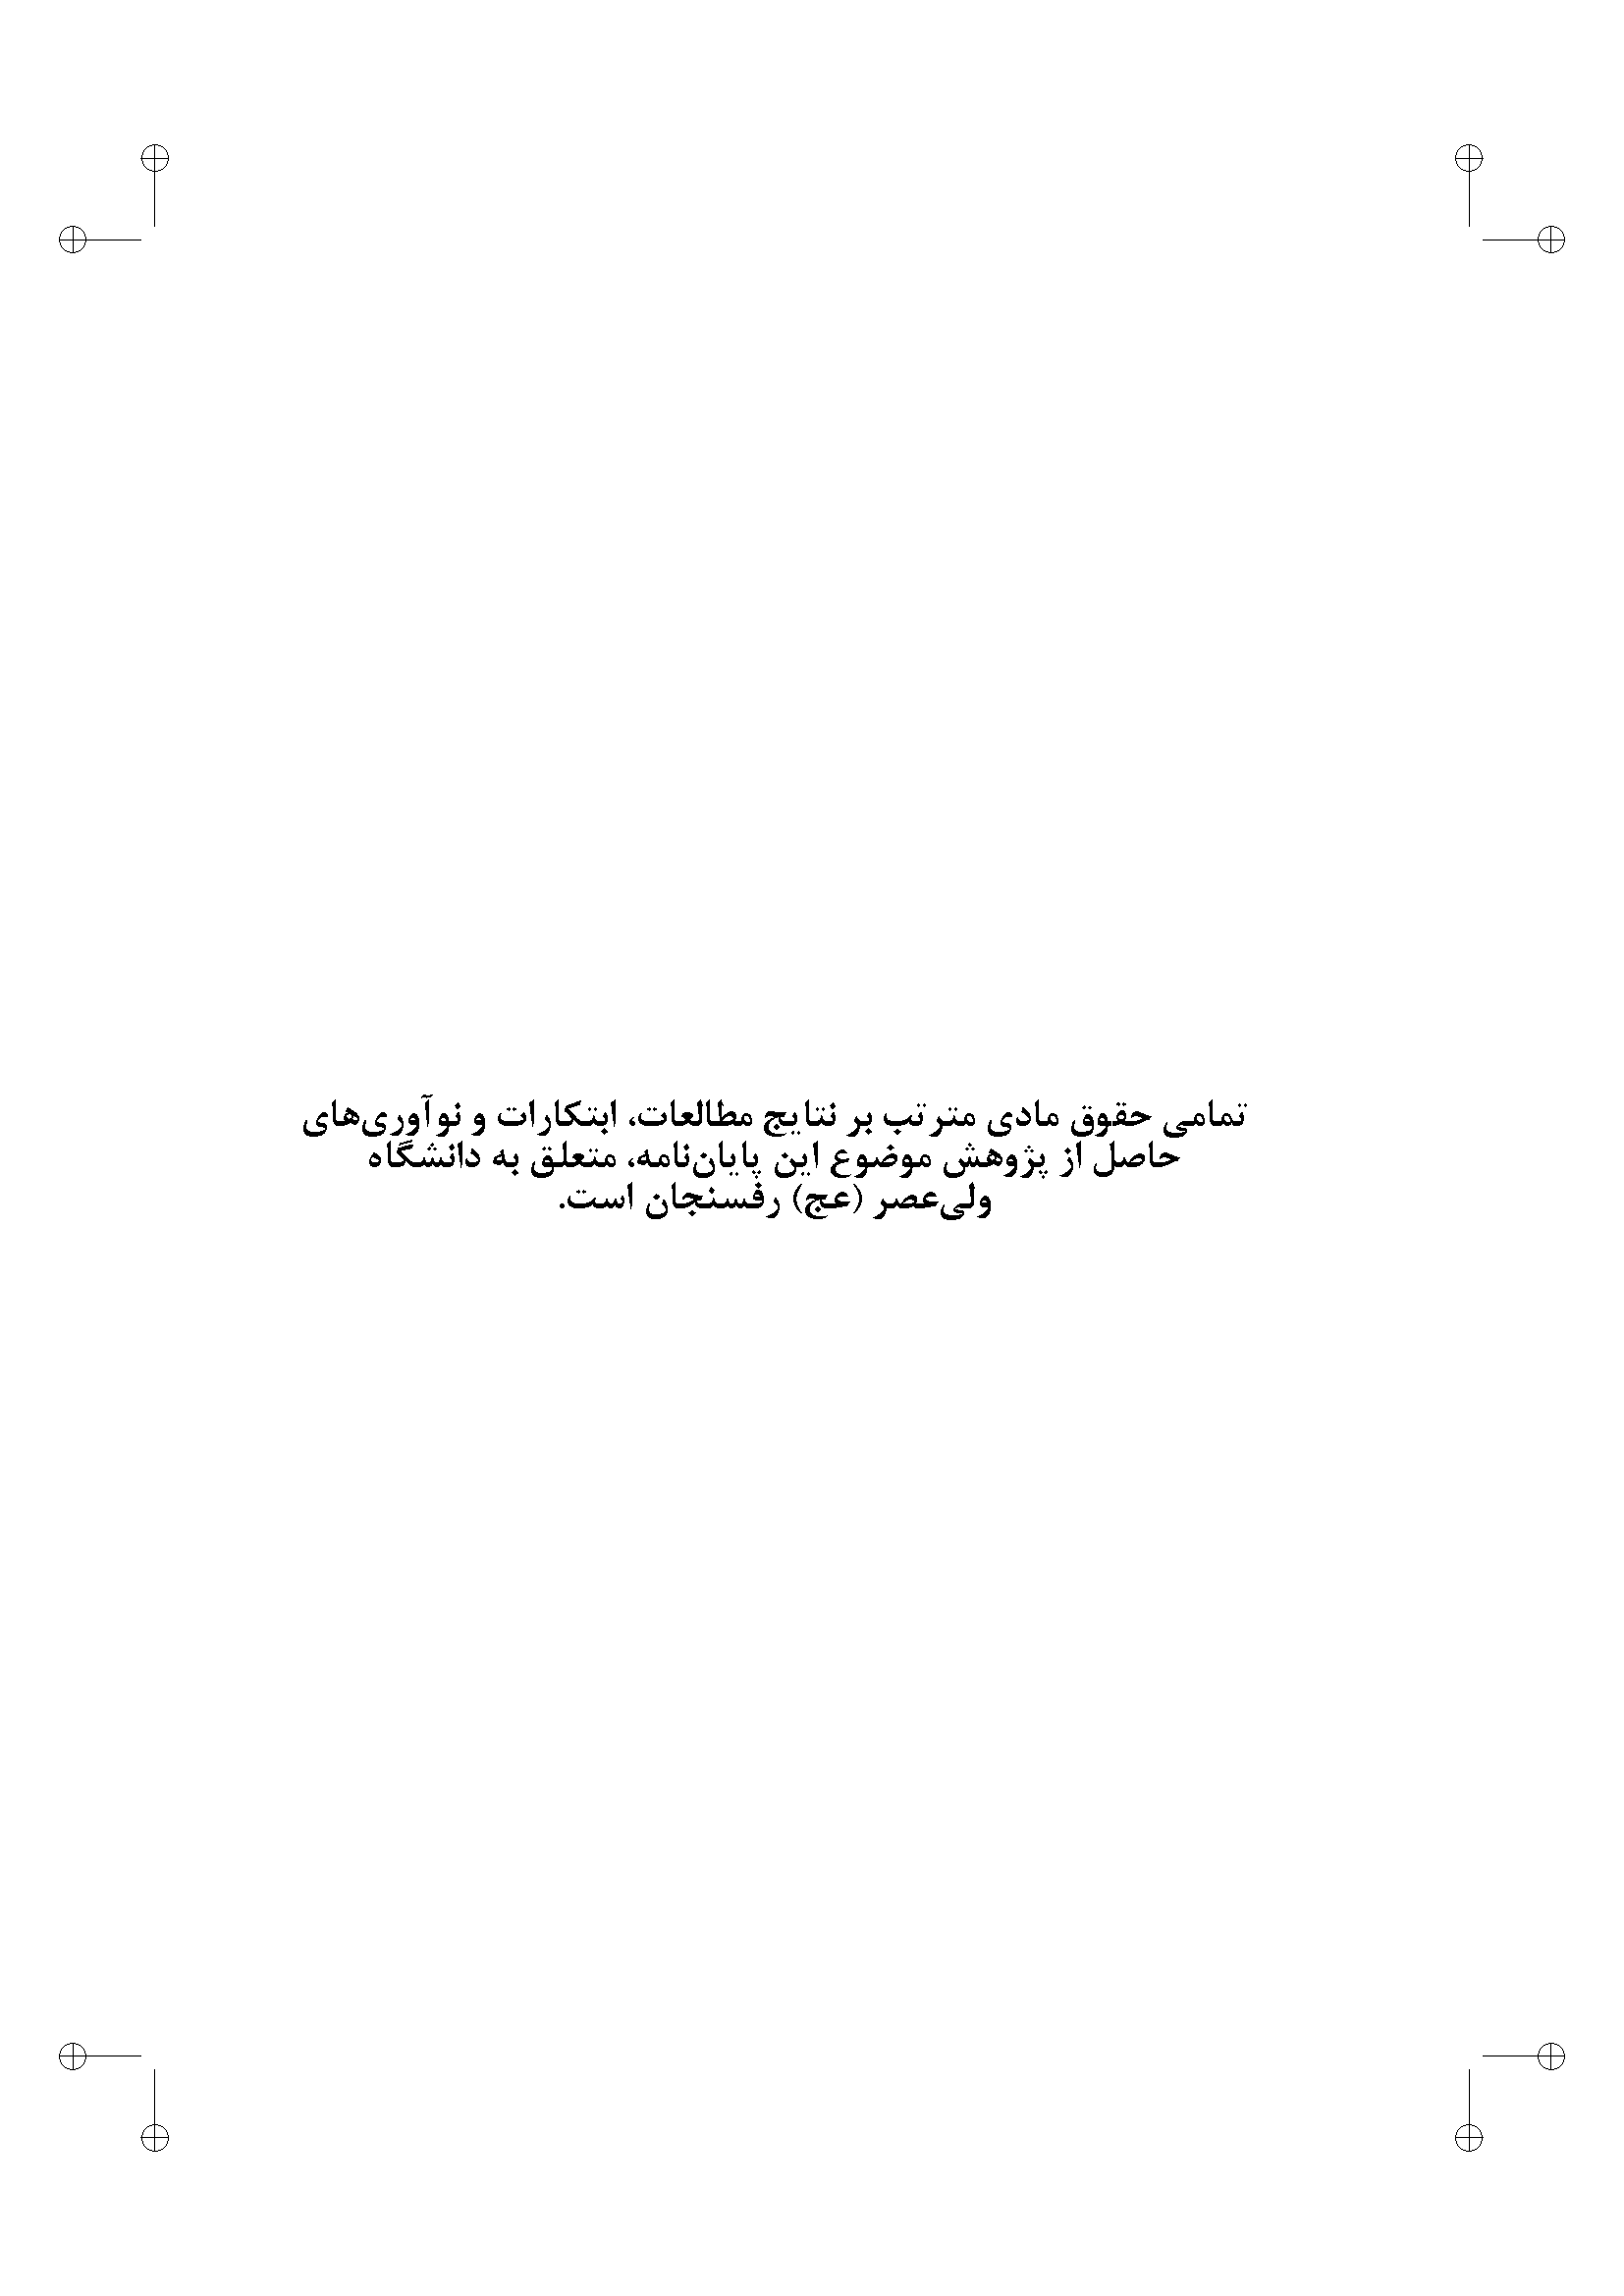
\includegraphics[width=\textwidth]{d.png}
		\caption{تعهدات حقوقی.}
		\label{app4}
	\end{figure}

	\begin{figure}
		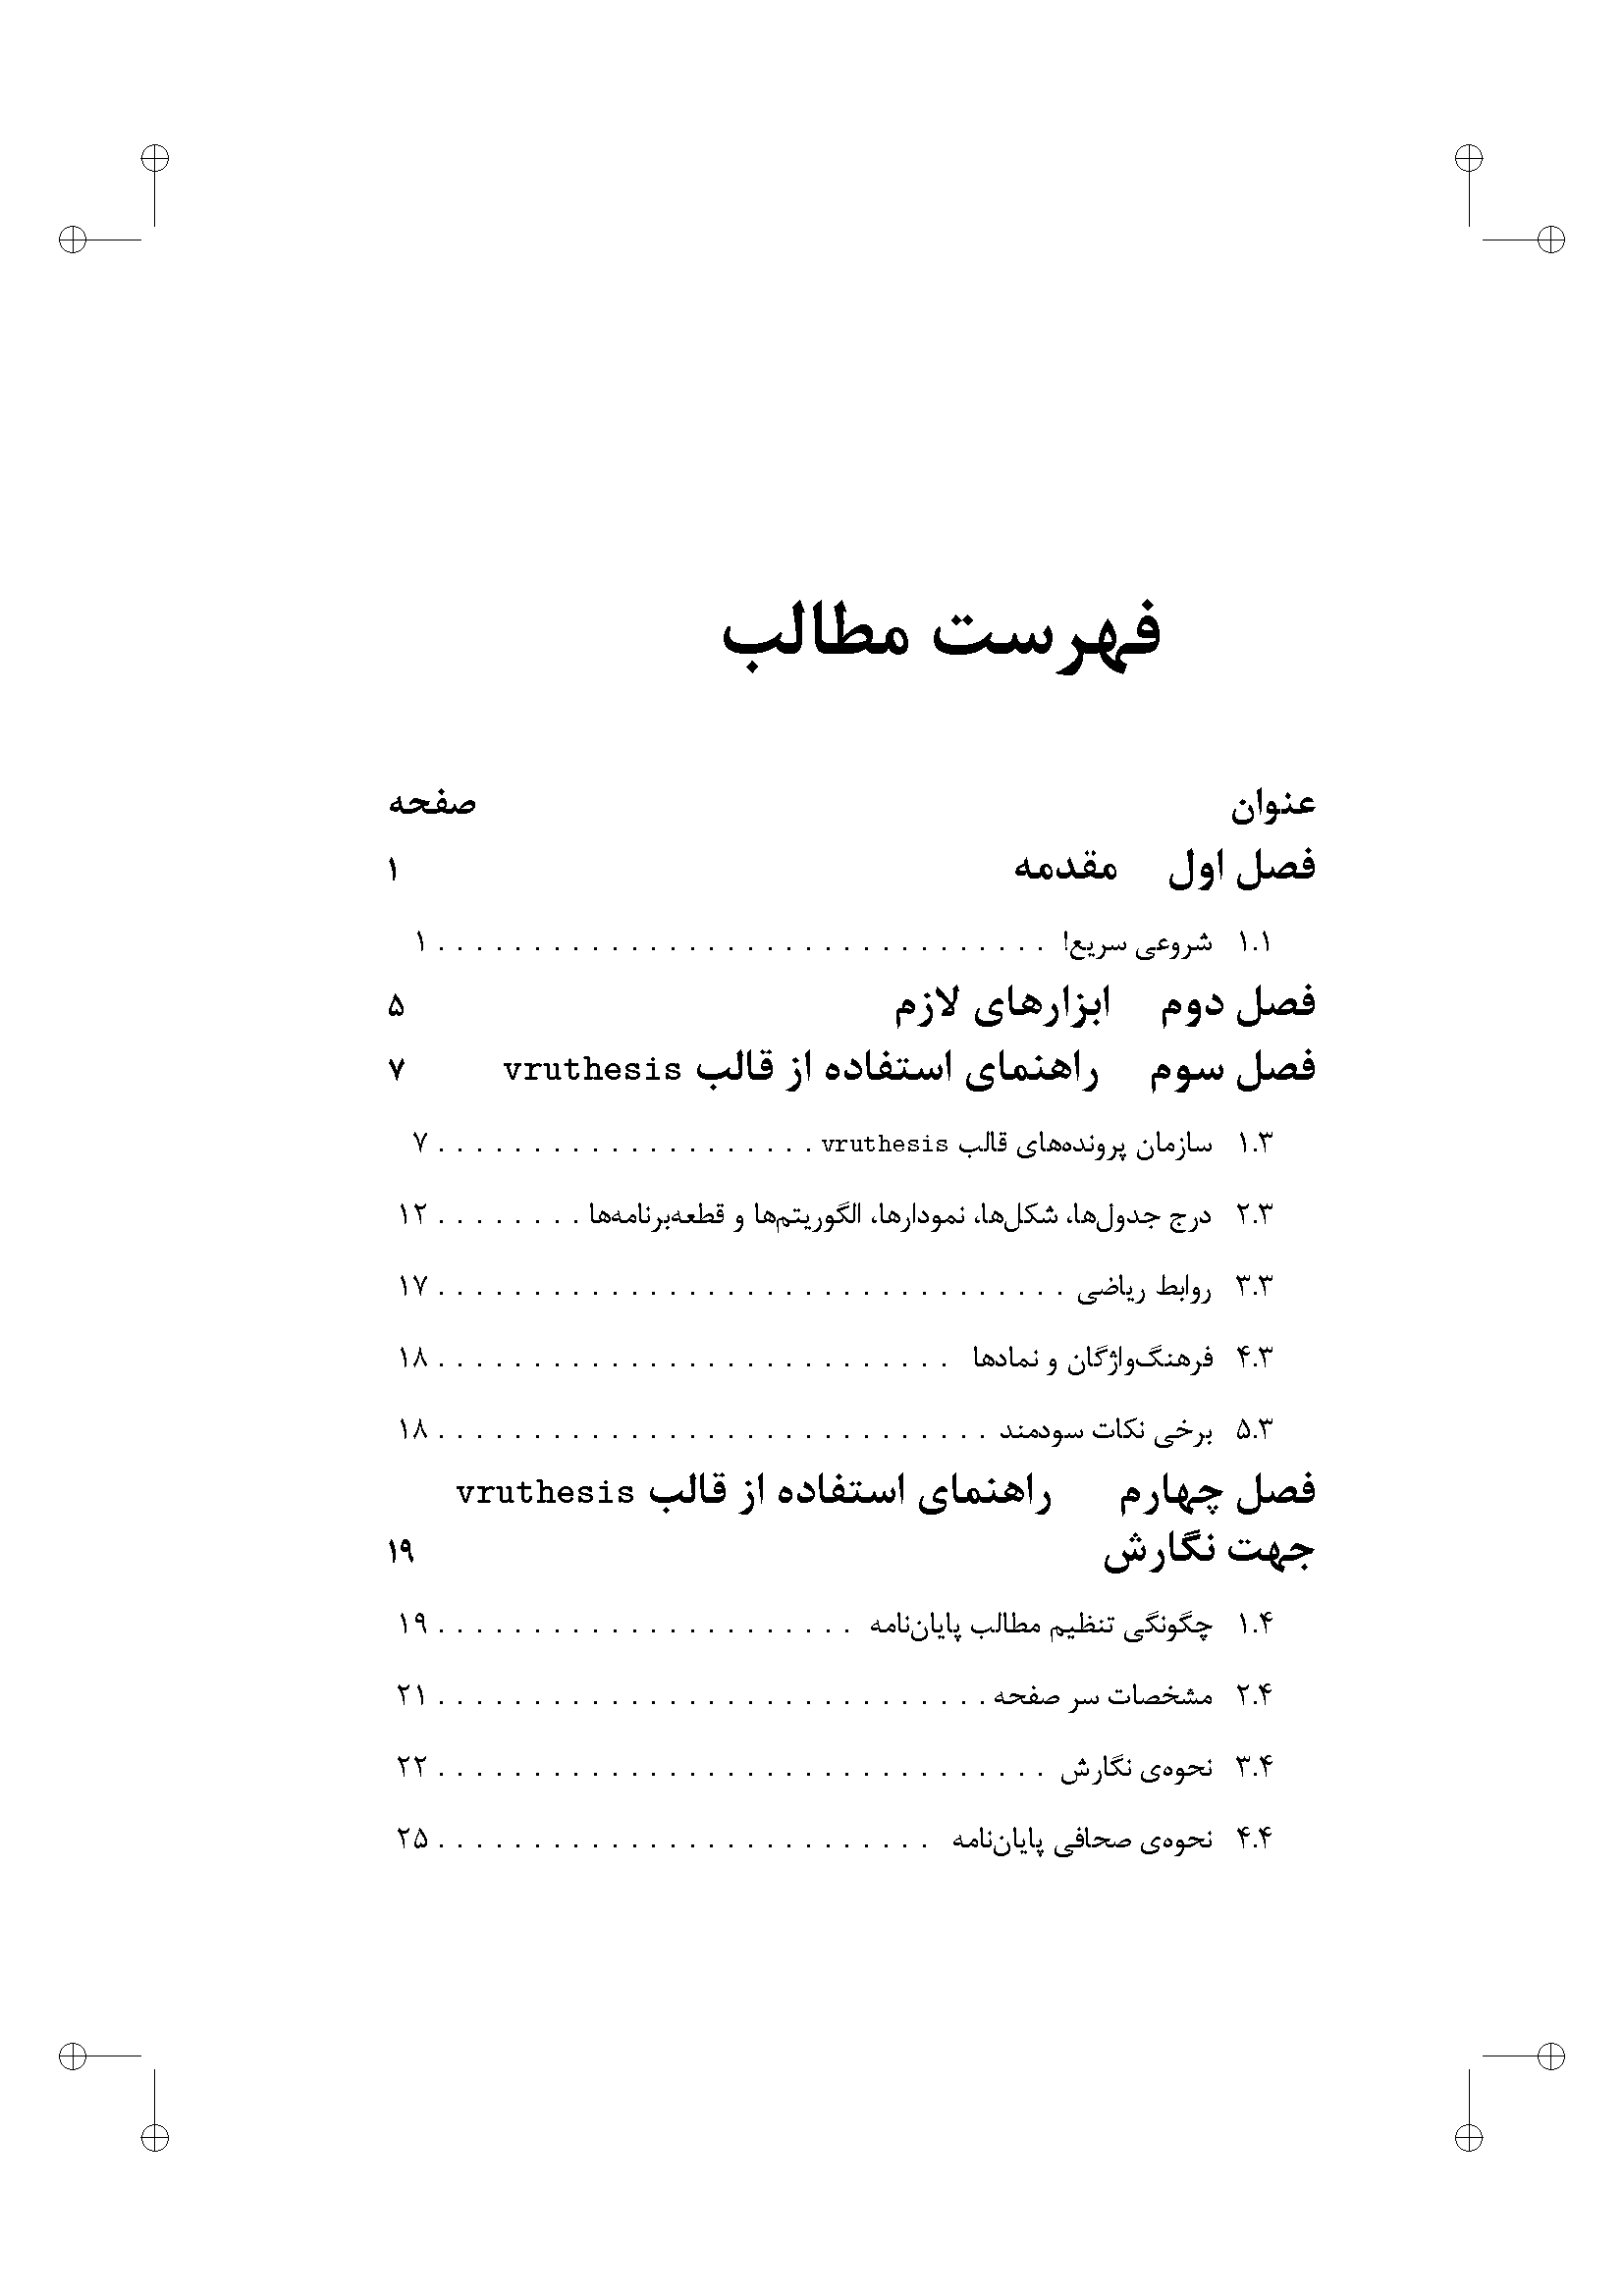
\includegraphics[width=\textwidth]{e.png}
		\caption{نمونه‌ای از فهرست مطالب.}
		\label{app5}
	\end{figure}

	\begin{figure}
		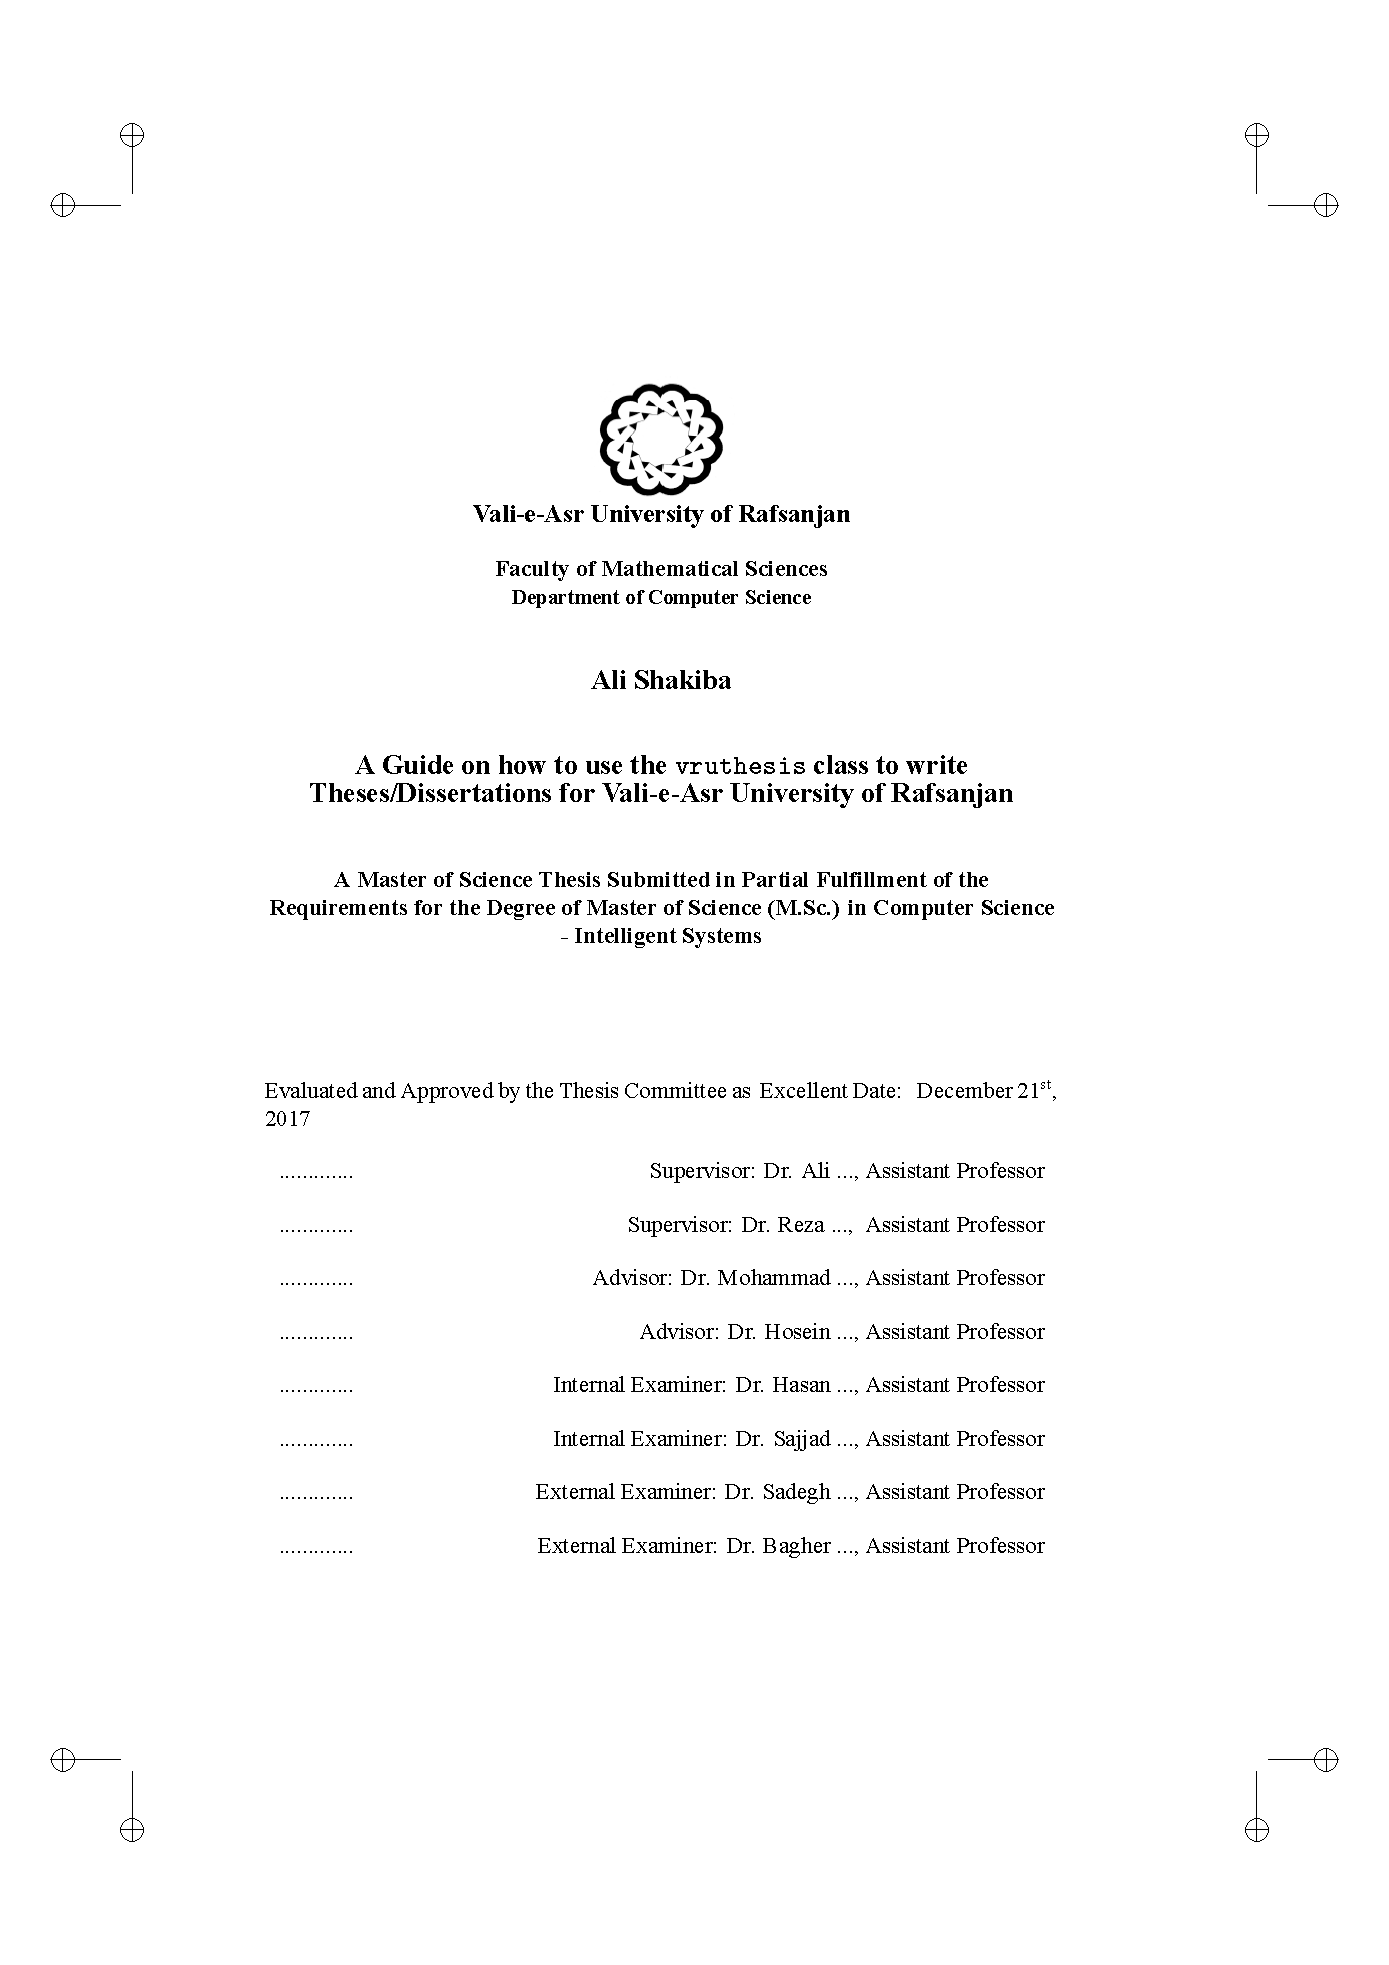
\includegraphics[width=\textwidth]{c.png}
		\caption{نمونه‌ی تصویب‌نامه‌ی پایان‌نامه‌ی کارشناسی ارشد به زبان انگلیسی.}
		\label{app3}
	\end{figure}

	\begin{figure}
		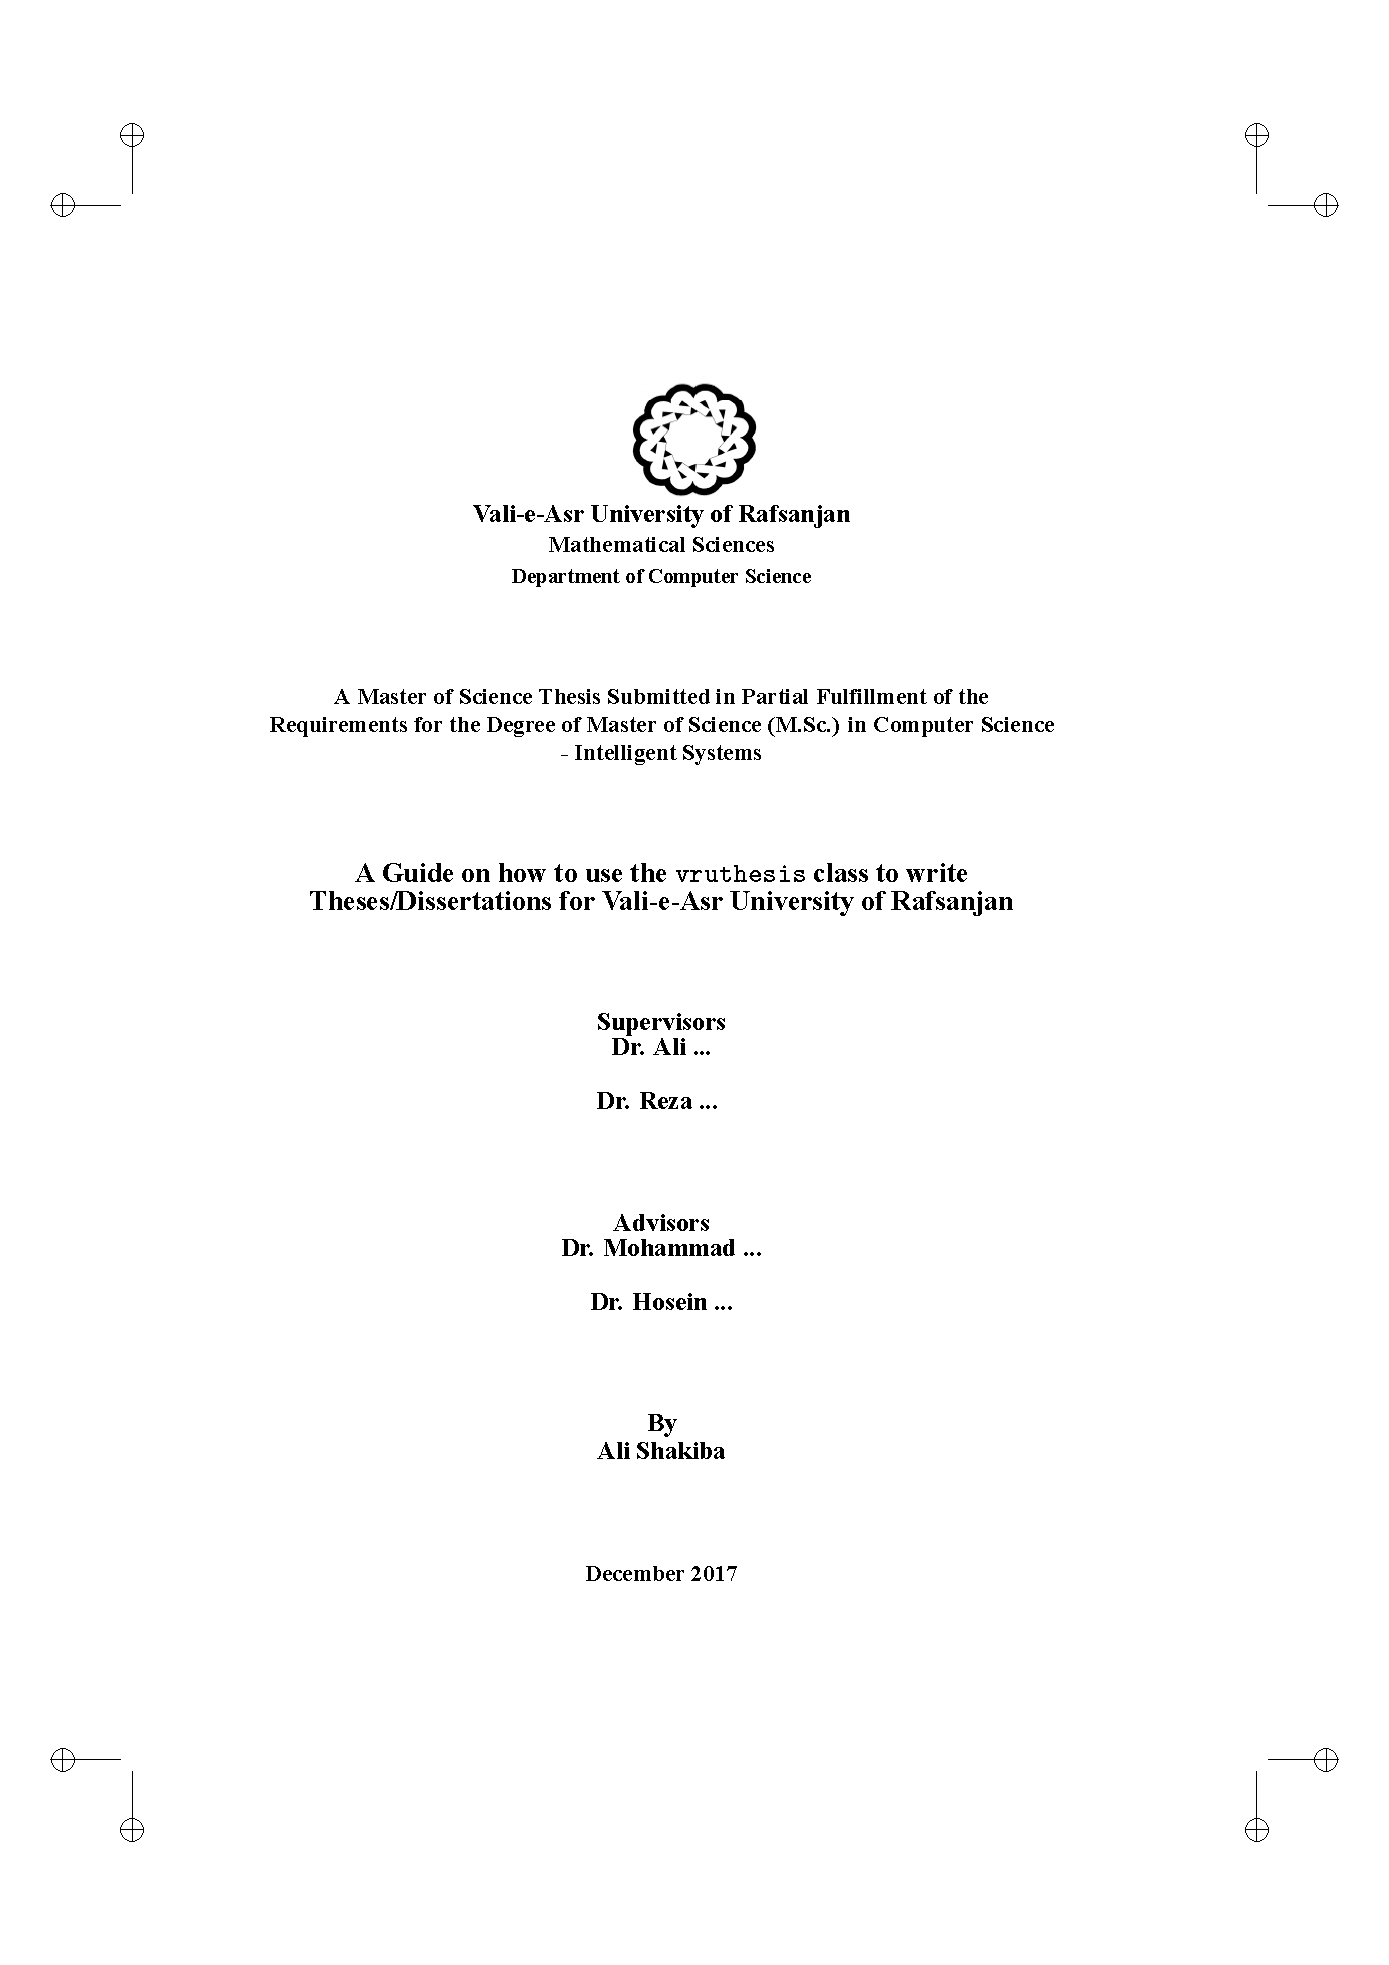
\includegraphics[width=\textwidth]{f.png}
		\caption{نمونه‌ی صفحه‌ی آخر پایان‌نامه‌ی کارشناسی ارشد.}
		\label{app6}
	\end{figure}
| قرار گیرد. 

	جهت تولید صفحات عنوان، ارزیابی، سپاسگزاری، تقدیم‌به و چکیده به هر دو زبان فارسی و انگلیسی، لازم است تا محتوای \gls{file} \texttt{data.tex} را به صورت مناسب، تکمیل کنید. دستورات مورد استفاده در این \gls{file} و کاربرد آن‌ها در جدول \ref{tbl:data_cmds} آمده‌اند. این دستورات ممکن است در نگاه اوّل گیج‌کننده به نظر برسند. به همین دلیل، توصیه می‌شود که از \gls{file} \verb|data.tex| در پایان‌نامه‌ی نمونه استفاده کرده و تنها محتویات خود را در آن، جایگزین نمایید. 
	
	\begin{longtable}[c]{| L{.45\textwidth} | R{.45\textwidth} |}
		\caption{دستورات قابل استفاده در \gls*{file} \texttt{thesis.tex}.}
	\label{tbl:data_cmds}
	\\
	\hline	
		\textbf{شرح} & \textbf{دستور} \\ \hline
	\endfirsthead
	\multicolumn{2}{c}{ادامه‌ی جدول \ref{tbl:data_cmds}.} \\ \hline
	\textbf{شرح} & \textbf{دستور} \\ \hline
	\endhead
		\multicolumn{2}{c}{ادامه‌ی جدول در صفحه‌ی بعد.} \\
	\endfoot
		\hline
	\multicolumn{2}{c}{پایان جدول \ref{tbl:data_cmds}.} \\ 
	\endlastfoot
	
		عنوان دانشکده به فارسی &  \verb|\faculty{}| \\ \hline
		عنوان دانشکده به انگلیسی &  \verb|\facultyen{}| \\ \hline
		نام گروه به فارسی &  \verb|\department{}| \\ \hline
		نام گروه به انگلیسی &  \verb|\departmenten{}| \\ \hline
		عنوان رشته‌ی تحصیلی به فارسی &  \verb|\subject{}| \\ \hline
		عنوان رشته‌ی تحصیلی به انگلیسی &  \verb|\subjecten{}| \\ \hline
		عنوان گرایش تحصیلی به فارسی &  \verb|\field{}| \\ \hline
		عنوان گرایش تحصیلی به انگلیسی &  \verb|\fielden{}| \\ \hline
		عنوان پایان‌نامه به فارسی &  \verb|\title{}| \\ \hline
		عنوان پایان‌نامه به انگلیسی &  \verb|\titleen{}| \\ \hline
		نام و نام خانوادگی استاد راهنما به فارسی با پیشوند «دکتر» &  \verb|\firstsupervisor{}| \\ \hline
		نام و نام خانوادگی استاد راهنما به انگلیسی با پیشوند «\lr{Dr.}» &  \verb|\firstsupervisoren{}| \\ \hline
		رتبه‌ی علمی استاد راهنما به فارسی &  \verb|\firstsupervisorrank{}| \\ \hline
		رتبه‌ی علمی استاد راهنما به انگلیسی &  \verb|\firstsupervisorranken{}| \\ \hline
		نام و نام خانوادگی استاد راهنمای دوم، در صورت وجود، به فارسی با پیشوند «دکتر» &  \verb|\secondsupervisor{}| \\ \hline
		نام و نام خانوادگی استاد راهنمای دوم، در صورت وجود، به انگلیسی با پیشوند «\lr{Dr.}» &  \verb|\secondsupervisoren{}| \\ \hline
		رتبه‌ی علمی استاد راهنمای دوم، در صورت وجود، به فارسی &  \verb|\secondsupervisorrank{}| \\ \hline
		رتبه‌ی علمی استاد راهنمای دوم، در صورت وجود، به انگلیسی &  \verb|\secondsupervisorranken{}| \\ \hline
		نام و نام خانوادگی استاد مشاور، در صورت وجود، به فارسی با پیشوند «دکتر» &  \verb|\firstadvisor{}| \\ \hline
		نام و نام خانوادگی استاد مشاور، در صورت وجود، به انگلیسی با پیشوند «\lr{Dr.}» &  \verb|\firstadvisoren{}| \\ \hline
		رتبه‌ی علمی استاد مشاور، در صورت وجود، به فارسی &  \verb|\firstadvisorrank{}| \\ \hline
		رتبه‌ی علمی استاد مشاور، در صورت وجود، به انگلیسی &  \verb|\firstadvisorranken{}| \\ \hline
		نام و نام خانوادگی استاد مشاور دوم، در صورت وجود، به فارسی با پیشوند «دکتر» &  \verb|\secondadvisor{}| \\ \hline
		نام و نام خانوادگی استاد مشاور دوم، در صورت وجود، به انگلیسی با پیشوند «\lr{Dr.}» &  \verb|\secondadvisoren{}| \\ \hline
		رتبه‌ی علمی استاد مشاور دوم، در صورت وجود، به فارسی &  \verb|\secondadvisorrank{}| \\ \hline
		رتبه‌ی علمی استاد مشاور دوم، در صورت وجود، به انگلیسی &  \verb|\secondadvisorranken{}| \\ \hline
		نام و نام خانوادگی استاد داور داخلی اول به فارسی با پیشوند «دکتر» &  \verb|\firstinternalreferee{}| \\ \hline
		نام و نام خانوادگی استاد داور داخلی اول به انگلیسی با پیشوند «\lr{Dr.}» &  \verb|\firstinternalrefereeen{}| \\ \hline
		رتبه‌ی علمی استاد داور داخلی اول به فارسی &  \verb|\firstinternalrefereerank{}| \\ \hline
		رتبه‌ی علمی استاد داور داخلی اول به انگلیسی &  \verb|\firstinternalrefereeranken{}| \\ \hline
		نام و نام خانوادگی استاد داور داخلی دوم، در صورت وجود، به فارسی با پیشوند «دکتر» &  \verb|\secondinternalreferee{}| \\ \hline
		نام و نام خانوادگی استاد داور داخلی دوم، در صورت وجود، به انگلیسی با پیشوند «\lr{Dr.}» &  \verb|\secondinternalrefereeen{}| \\ \hline
		رتبه‌ی علمی استاد داور داخلی دوم، در صورت وجود، به فارسی &  \verb|\secondinternalrefereerank{}| \\ \hline
		رتبه‌ی علمی استاد داور داخلی دوم، در صورت وجود، به انگلیسی &  \verb|\secondinternalrefereeranken{}| \\ \hline
		نام و نام خانوادگی استاد داور خارجی اول به فارسی با پیشوند «دکتر» &  \verb|\firstexternalreferee{}| \\ \hline
		نام و نام خانوادگی استاد داور خارجی اول به انگلیسی با پیشوند «\lr{Dr.}» &  \verb|\firstexternalrefereeen{}| \\ \hline
		رتبه‌ی علمی استاد داور خارجی اول به فارسی &  \verb|\firstexternalrefereerank{}| \\ \hline
		رتبه‌ی علمی استاد داور خارجی اول به انگلیسی &  \verb|\firstexternalrefereeranken{}| \\ \hline
		نام و نام خانوادگی استاد داور خارجی دوم، در صورت وجود، به فارسی با پیشوند «دکتر» &  \verb|\secondexternalreferee{}| \\ \hline
		نام و نام خانوادگی استاد داور خارجی دوم، در صورت وجود، به انگلیسی با پیشوند «\lr{Dr.}» &  \verb|\secondexternalrefereeen{}| \\ \hline
		رتبه‌ی علمی استاد داور خارجی دوم، در صورت وجود، به فارسی &  \verb|\secondexternalrefereerank{}| \\ \hline
		رتبه‌ی علمی استاد داور خارجی دوم، در صورت وجود، به انگلیسی &  \verb|\secondexternalrefereeranken{}| \\ \hline
		نام و نام خانوادگی استاد ناظر به فارسی با پیشوند «دکتر» &  \verb|\viewer{}| \\ \hline
		نام و نام خانوادگی استاد ناظر به انگلیسی با پیشوند «\lr{Dr.}» &  \verb|\vieweren{}| \\ \hline
		رتبه‌ی علمی استاد ناظر به فارسی &  \verb|\viewerrank{}| \\ \hline
		رتبه‌ی علمی استاد ناظر به انگلیسی &  \verb|\viewerranken{}| \\ \hline
		نام دانشجو به فارسی &  \verb|\name{}| \\ \hline
		نام دانشجو به انگلیسی &  \verb|\nameen{}| \\ \hline
		نام خانوادگی دانشجو به فارسی &  \verb|\surname{}| \\ \hline
		نام خانوادگی دانشجو به انگلیسی &  \verb|\surnameen{}| \\ \hline
		ماه و سال جلسه‌ی دفاع به تقویم شمسی، مانند آذر $1396$ &  \verb|\thesisdate{}| \\ \hline
		ماه و سال جلسه‌ی دفاع به تقویم میلادی، مانند \lr{December 2017} &  \verb|\thesisdateen{}| \\ \hline
		تعداد واحد پایان‌نامه به فارسی، مانند $6$ &  \verb|\credit{}| \\ \hline
		تعداد واحد پایان‌نامه به انگلیسی، مانند \lr{$6$} &  \verb|\crediten{}| \\ \hline
		تاریخ جلسه‌ی دفاع به تقویم شمسی، مانند $۱۳۹۶/۰۹/۳۰$ &  \verb|\defensedate{}| \\ \hline
		تاریخ جلسه‌ی دفاع به تقویم میلادی، مانند \lr{December 21${}^{\text{st}}$, 2017}  &  \verb|\defensedateen{}| \\ \hline
		نمره‌ی پایان‌نامه با اعداد فارسی مانند، $19.75$ &  \verb|\grade{}| \\ \hline
		نمره‌ی پایان‌نامه با اعداد انگلیسی مانند، \lr{$19.75$} &  \verb|\gradeen{}| \\ \hline
		نمره‌ی پایان‌نامه به حروف به زبان فارسی &  \verb|\letgrade{}| \\ \hline
		نمره‌ی پایان‌نامه به حروف به زبان انگلیسی  &  \verb|\letgradeen{}| \\ \hline
		درجه‌ی دفاع به فارسی &  \verb|\degree{}| \\ \hline
		درجه‌ی دفاع به انگلیسی &  \verb|\degreeen{}| \\ \hline
		متن تقدیم‌به به زبان فارسی &  \verb|\totext{}| \\ \hline
		متن سپاسگزاری به فارسی &  \verb|\ack{}| \\ \hline
		متن چکیده به فارسی &  \verb|\abstractfa{}| \\ \hline
		متن چکیده به انگلیسی &  \verb|\abstracten{}| \\ \hline
	\end{longtable}

		\section{درج جدول‌ها، شکل‌ها، نمودارها، الگوریتم‌ها و قطعه‌برنامه‌ها}\label{sec:figs_tbls_algs_codes}
		پایان‌نامه‌ی شما ممکن است دارای جدول‌ها، شکل‌ها، نمودارها، الگوریتم‌ها و قطعه‌برنامه‌های مختلفی باشد. در این قالب، سه نوع محتوا درنظر گرفته شده است:
		\begin{itemize}
			\item جدول که تنها برای نمایش جدول‌ها استفاده می‌شود.
				\item الگوریتم که تنها برای نمایش الگوریتم‌ها استفاده می‌شود. 
			\item شکل که برای نمایش نمودارها،  قطعه‌برنامه‌ها، \glspl{flowchart} و سایر موارد بصری مورد استفاده قرار می‌گیرد.
		\end{itemize}
		
		در ادامه، نمونه‌ای از هر یک از موارد فوق آمده است. جدول \ref{tbl1}، یک جدول با تعداد ستون‌های زیاد است که لازم است تا در صفحه‌ای جداگانه درج شود. قطعه کد تولیدکننده‌ی این جدول در شکل \ref{fig:tbl1} آمده است. 
		
			شکل \ref{fig:clus1} نمونه‌ای از یک خوشه‌بندی برای یک دادگان نمونه است. همچنین، الگوریتم \ref{fig:alg} نیز نمونه‌ای از یک الگوریتم را نشان می‌دهد. از شکل‌ها می‌توان به منظور نمایش نمودارها نیز استفاده کرد؛ مانند \ref{fig:chart}. همچنین، شکل \ref{fig:tbl1}، بیانگر یک قطعه‌کد در \lr{\LaTeX} است. 
			
			\begin{figure}
				\centering
				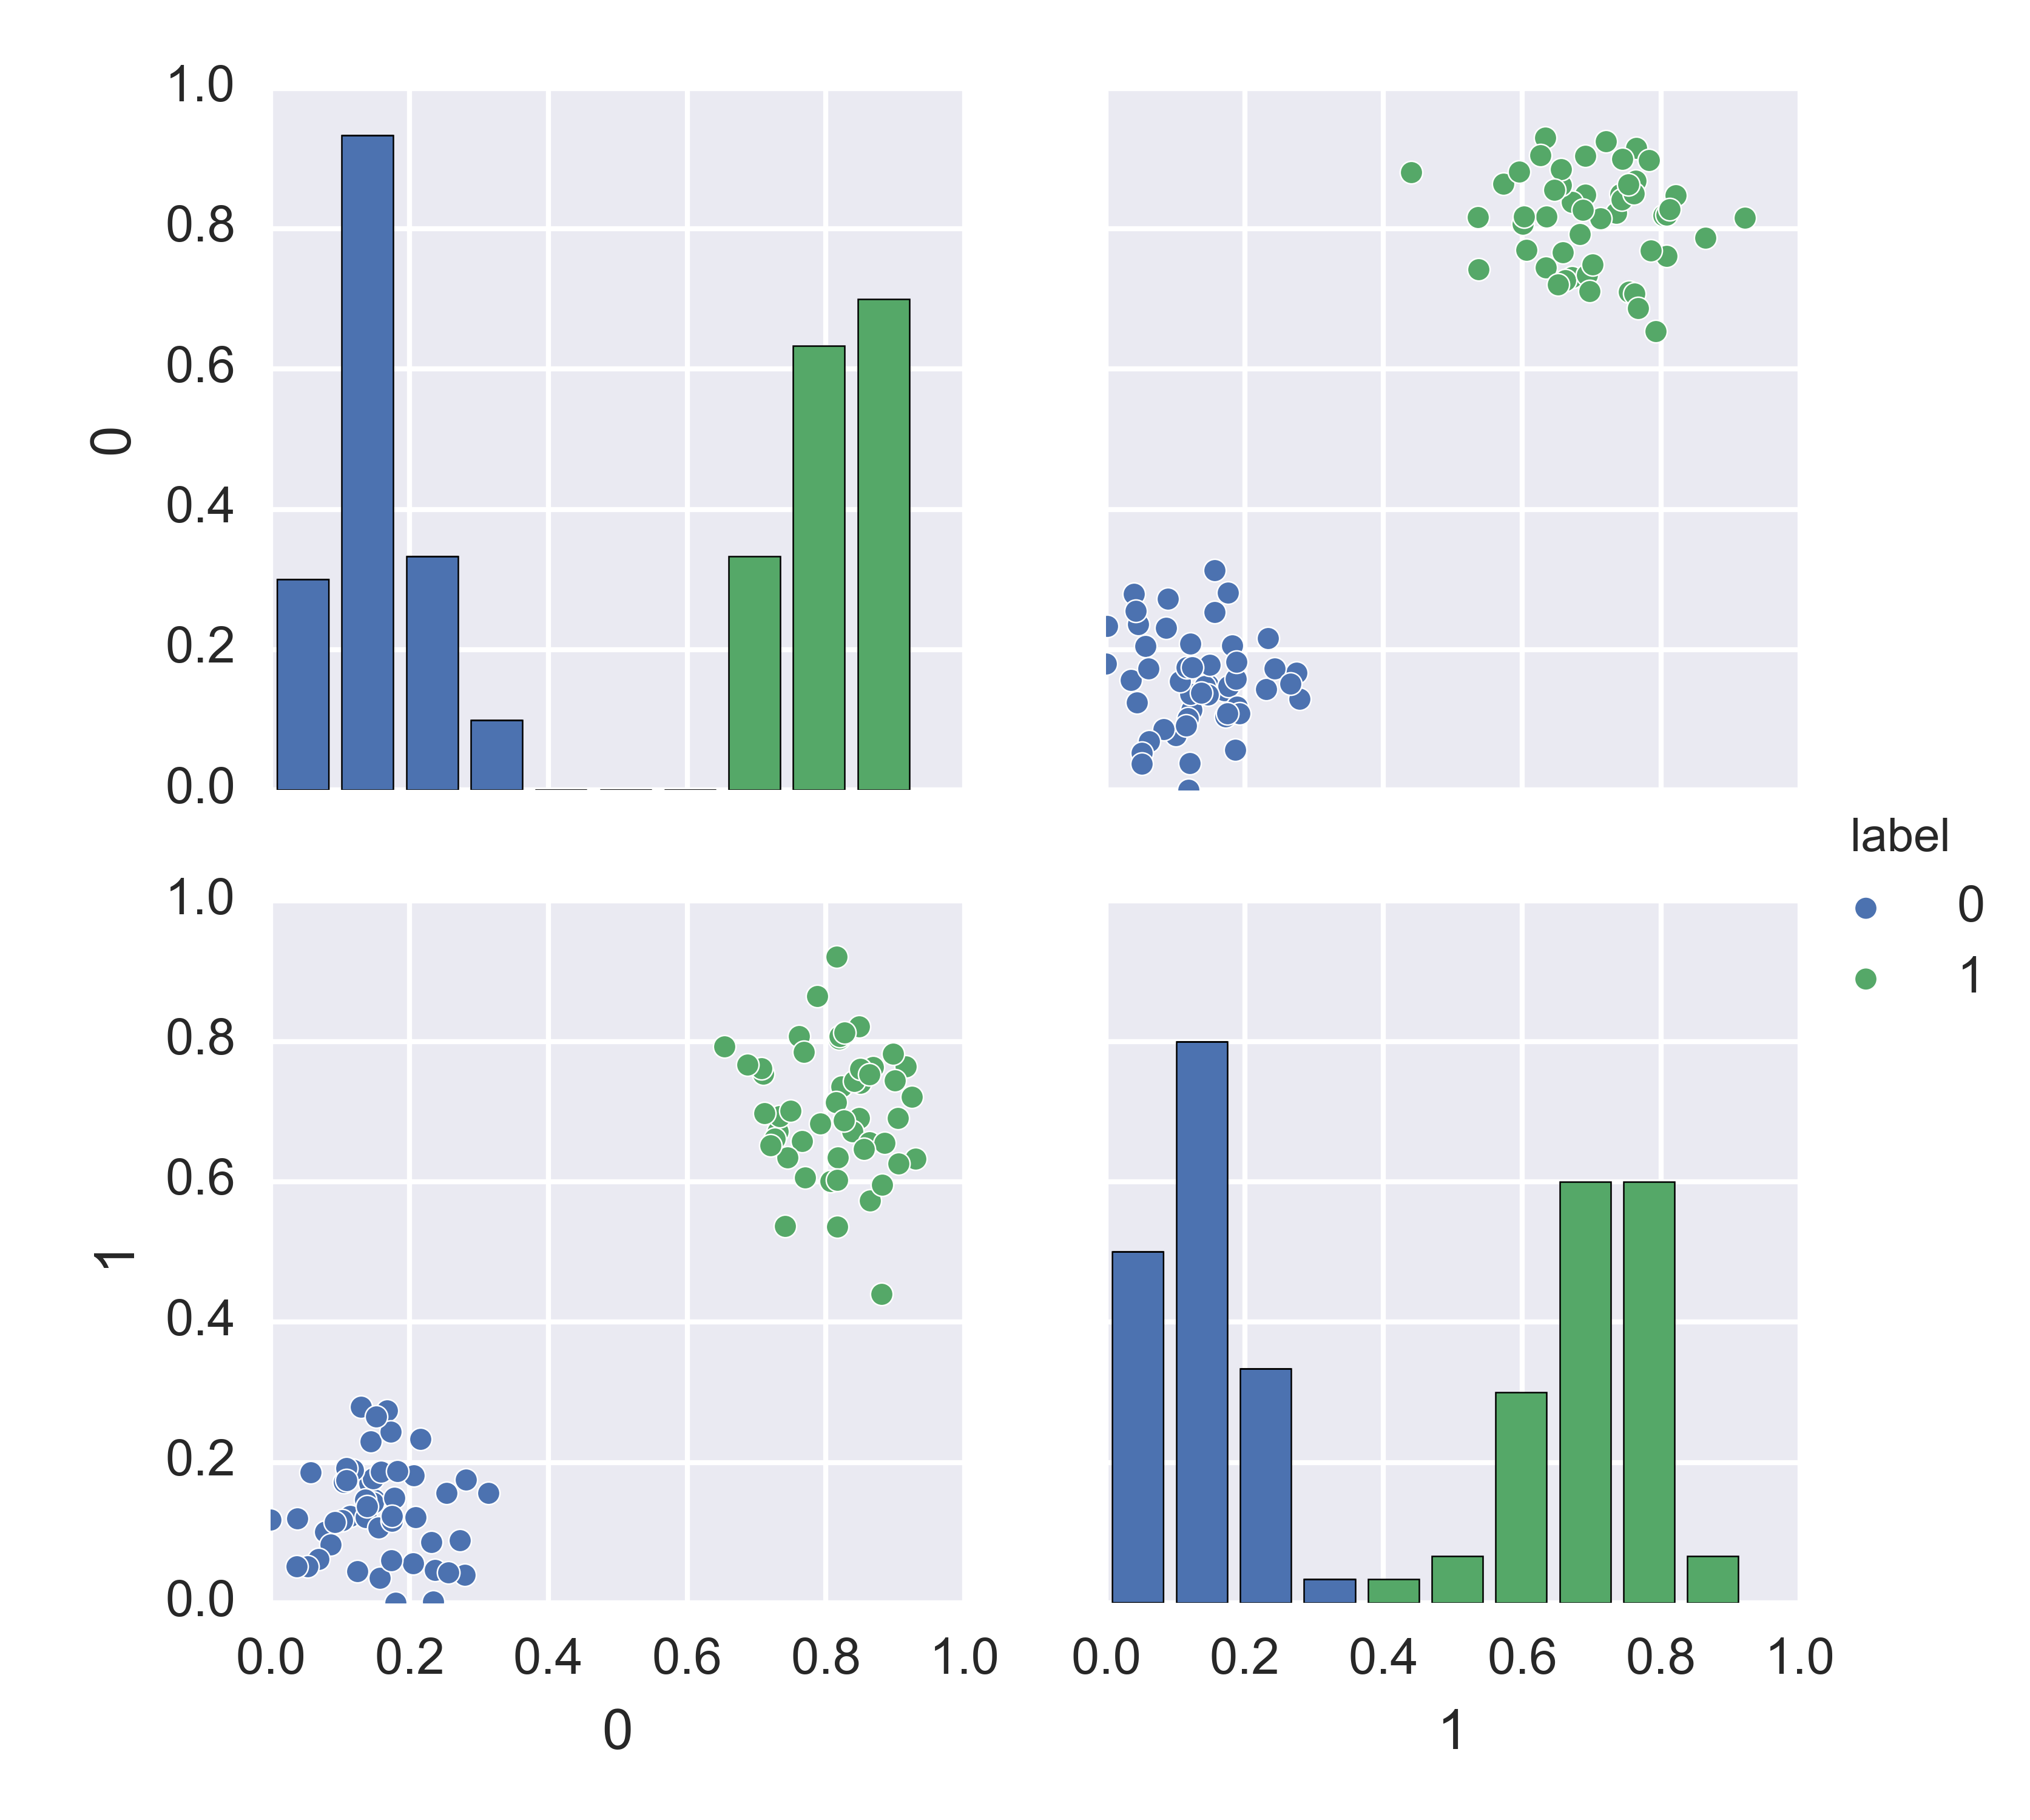
\includegraphics[width=.7\textwidth]{clus1}
				\caption{نمونه‌ای از یک خوشه‌بندی برای یک دادگان نمونه.}
				\label{fig:clus1}
			\end{figure}
		
		\begin{algorithm}
				\begin{latin}
		\begin{algorithmic}[1] % The number tells where the line numbering should start
        \Procedure{Euclid}{$a,b$} \Comment{\rl{ب.م.م. دو عدد صحیح مثبت $a$ و $b$}}
            \State $r\gets a \bmod b$
            \While{$r\not=0$} \Comment{\rl{اگر $r$ صفر باشد؛ پاسخ محاسبه شده است.}}
                \State $a \gets b$
                \State $b \gets r$
                \State $r \gets a \bmod b$
            \EndWhile\label{euclidendwhile}
            \State \textbf{return} $b$\Comment{\rl{ب.م.م. برابر با $b$ است.}}
        \EndProcedure
    \end{algorithmic}
    \end{latin}
    		\caption{الگوریتم اقلیدس برای محاسبه‌ی \gls*{gcd}.}
				\label{fig:alg}		
		\end{algorithm}	
			
			\begin{figure}
				\centering
				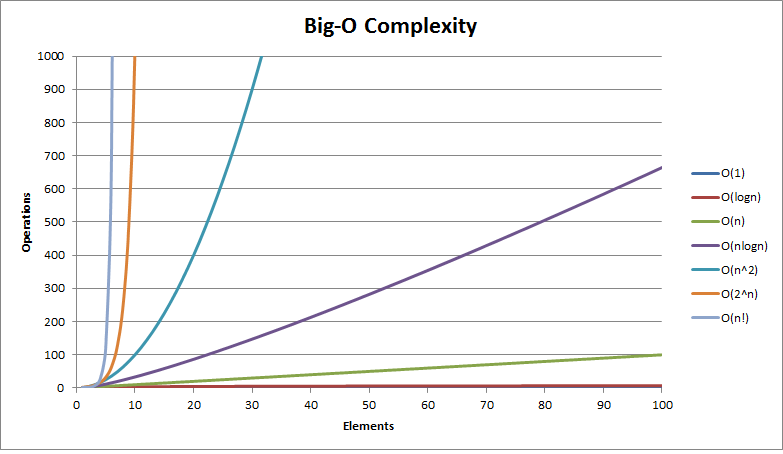
\includegraphics[width=.7\textwidth]{chart}
				\caption{نمونه‌ای از یک نمودار.}
				\label{fig:chart}
			\end{figure}
		
		\begin{figure}
			\centering
		\footnotesize
		\begin{myverbatim}
\begin{landscape}
  \begin{table}
    \caption{+rl[نمونه‌ای از یک جدول با تعداد ستون‌های زیاد.]}
    \label{tbl1}
    \centering
    \footnotesize
    \begin{tabular}{|r||c|c|c|c|c|c|c|c|c|c|c|c|c|c|c|}
      \hline
      \textbf{+rl[عنوان]} & $\alpha$ 
        & \multicolumn{5}{|c|}{$\gamma_1, \gamma_2, \ldots, \gamma_5$} 
        & $\beta$ & \multicolumn{8}{|c|}{+rl[سایر پارامترها]} \\ \hline
      +rl[نمونه‌ی اول]   &   74.85 &  0.32 &  13.99 &  91.25 &  80.74
         &  15.44 &  74.49 &  42.13 &
        1.08  &  32.98 &  18.74 &  46.83 &  81.28 &  31.52 &  8.29 \\
      +rl[نمونه‌ی دوم] &   22.76 &  48.61 &  
        70.77 &  22.77 &  3.81 &  45.05 &  
        70.55 &  33.20 &  1.40  &  24.42 &  79.06 &  
          30.38 &  24.95 &  19.77 &  44.59 \\
      +rl[نمونه‌ی سوم] &   55.67 &  36.98 &
          89.61 &  56.43 &  88.97 &  38.21 &  
        81.40 &  77.05 &  9.35 &  18.52 &  3.48 &  
          95.93 &  9.20 &  16.30 &  84.36 \\
      +rl[نمونه‌ی چهارم] &   60.31 &  88.25 &
          29.96 &  56.83 &  89.49 &  38.26 &  
        55.73 &  99.36 &  21.70 &  74.46 &  49.11 &  2.82
           &  25.47 &  2.90 &  84.58 \\
      +rl[نمونه‌ی پنجم] &   90.17 &  51.53 
        &  32.67 &  82.55 &  87.72 &  66.09 &  26.86 &  
        4.69 &  77.97 &  40.23 &  58.59 &  70.13 &  70.23 &
            80.73 &  64.88 \\
      +rl[نمونه‌ی ششم] &   74.92 
        &  52.33 &  98.68 &  63.75 &  30.10 &  7.32 &  91.70 &  
        72.76 &  42.50 &  26.72 &  23.33 &  73.55 & 
           77.37 &  32.79 &  15.60 \\
      +rl[نمونه‌ی هفتم] &   26.85 &  55.27
         &  5.12 &  88.21 &  4.92 &  70.78 &  
        75.26 &  32.03 &  25.11 &  61.81 &  44.24 &
            47.14 &  98.98 &  16.90 &  20.27 \\
      +rl[نمونه‌ی هشتم] &   84.33 &  12.53 &  36.00
         &  24.02 &  44.60 &  8.44 &  
        5.73 &  10.37 &  16.94 &  15.41 &  39.69 &
            43.74 &  10.43 &  73.96 &  26.51 \\
      +rl[نمونه‌ی نهم] &   59.21 &  47.46 & 
           97.27 &  87.05 &  84.65 &  17.95 &  50.05 &  
        38.68 &  20.09 &  46.99 &  12.47 &  10.92 & 
           78.38 &  74.53 &  31.83 \\
      +rl[نمونه‌ی دهم] &   97.61 &  33.47 &  67.78 
        &  69.95 &  60.95 &  88.40 &  
        59.64 &  18.22 &  57.49 &  97.76 &  40.31 &
            4.83 &  8.90 &  69.18 &  97.02 \\ \hline
    \end{tabular}
  \end{table}
\end{landscape}
		\end{myverbatim}
		\caption{قطعه‌کد مربوط به تولید جدول \ref{tbl1}.}
		\label{fig:tbl1}
		\end{figure}
	
	
		
		\begin{landscape}
			\begin{table}
				\caption{نمونه‌ای از یک جدول با تعداد ستون‌های زیاد.}
				\label{tbl1}
				\centering
				\footnotesize
				\begin{tabular}{|r||c|c|c|c|c|c|c|c|c|c|c|c|c|c|c|}
				\hline
				\textbf{عنوان} & $\alpha$ & \multicolumn{5}{|c|}{$\gamma_1, \gamma_2, \ldots, \gamma_5$} & $\beta$ & \multicolumn{8}{|c|}{سایر پارامترها} \\ \hline
نمونه‌ی اول 	&   74.85 &  0.32 &  13.99 &  91.25 &  80.74 &  15.44 &  74.49 &  42.13 &  1.08  &  32.98 &  18.74 &  46.83 &  81.28 &  31.52 &  8.29 \\
نمونه‌ی دوم &   22.76 &  48.61 &  70.77 &  22.77 &  3.81 &  45.05 &  70.55 &  33.20 &  1.40  &  24.42 &  79.06 &  30.38 &  24.95 &  19.77 &  44.59 \\
نمونه‌ی سوم &   55.67 &  36.98 &  89.61 &  56.43 &  88.97 &  38.21 &  81.40 &  77.05 &  9.35 &  18.52 &  3.48 &  95.93 &  9.20 &  16.30 &  84.36 \\
نمونه‌ی چهارم &   60.31 &  88.25 &  29.96 &  56.83 &  89.49 &  38.26 &  55.73 &  99.36 &  21.70 &  74.46 &  49.11 &  2.82 &  25.47 &  2.90 &  84.58 \\
نمونه‌ی پنجم &   90.17 &  51.53 &  32.67 &  82.55 &  87.72 &  66.09 &  26.86 &  4.69 &  77.97 &  40.23 &  58.59 &  70.13 &  70.23 &  80.73 &  64.88 \\
نمونه‌ی ششم &   74.92 &  52.33 &  98.68 &  63.75 &  30.10 &  7.32 &  91.70 &  72.76 &  42.50 &  26.72 &  23.33 &  73.55 &  77.37 &  32.79 &  15.60 \\
نمونه‌ی هفتم &   26.85 &  55.27 &  5.12 &  88.21 &  4.92 &  70.78 &  75.26 &  32.03 &  25.11 &  61.81 &  44.24 &  47.14 &  98.98 &  16.90 &  20.27 \\
نمونه‌ی هشتم &   84.33 &  12.53 &  36.00 &  24.02 &  44.60 &  8.44 &  5.73 &  10.37 &  16.94 &  15.41 &  39.69 &  43.74 &  10.43 &  73.96 &  26.51 \\
نمونه‌ی نهم &   59.21 &  47.46 &  97.27 &  87.05 &  84.65 &  17.95 &  50.05 &  38.68 &  20.09 &  46.99 &  12.47 &  10.92 &  78.38 &  74.53 &  31.83 \\
نمونه‌ی دهم &   97.61 &  33.47 &  67.78 &  69.95 &  60.95 &  88.40 &  59.64 &  18.22 &  57.49 &  97.76 &  40.31 &  4.83 &  8.90 &  69.18 &  97.02 \\ \hline
				\end{tabular}
			\end{table}
		\end{landscape}
	
		\section{روابط ریاضی}\label{sec:eqs}
		به طور معمول، بخش زیادی از یک پایان‌نامه در دانشکده‌ی علوم ریاضی، از روابط ریاضی تشکیل شده است. یک رابطه‌ی ریاضی را می‌توان به صورت \gls{inline} مانند $\int_{-\infty}^{+\infty} \sin x \mathrm{d} x$ نوشت. همچنین، می‌توان یک رابطه‌ی ریاضی را بدون شماره‌گذاری مانند
		$$
			A \wedge \left( B \vee C \right) = \left(A \wedge B \right) \vee \left( A \wedge C \right),
		$$
		نوشت. امّا، با توجه به زیادبودن تعداد روابط ریاضی، بهتر است در صورتی که به یک رابطه ارجاع داده می‌شود؛ آن را شماره‌گذاری نمایید؛ مانند
		\begin{equation}
			P \left(B_i \vert A \right) = \frac{P\left(A \vert B_i \right) P\left(B_i\right)}{\sum_j P\left(A \vert B_j \right) P\left(B_j\right)},
			\label{eq:1}
		\end{equation}
		که $i=1,\ldots,k$ است. بنابراین، می‌توان به سادگی به رابطه‌ی \ref{eq:1}، ارجاع داد. 
		
		همچنین، محیط‌های متنوعی برای \gls{typeset} قضیه‌ها، لم‌ها، گزاره‌ها، نتیجه‌ها، تعریف‌ها و مانند آن‌ها در نظر گرفته شده‌اند که در ادامه، نمونه‌های مختلفی از آن‌ها را مشاهده می‌کنید.
		
		\begin{theorem}[\cite{gary}]
			\label{}
			زبان $\mathrm{SAT} = \left\{ \left\langle \Phi \right\rangle \ \vert \ \text{\rl{ صدق‌پذیر است} } \Phi  \right\}$، مفروض است. داریم
			\begin{equation}
				\mathrm{SAT} \in \mathbf{NP}\mathrm{-complete}.
			\end{equation}
		\end{theorem}
		\begin{proof}
			برای اثبات می‌توان به مرجع \cite{gary} مراجعه نمود. 
		\end{proof}
		
		\begin{definition}[ضخامت گراف]
			ضخامت گراف $G$ عبارت است از حداقل تعداد گراف‌های مسطح ممکن در تجزیه‌ی $G$ به گراف‌های مسطح.
		\end{definition}
		
		\begin{lemma}{قضیه‌ی پنج رنگ \cite{heawood1890}}
			هر گراف مسطح، قابل $5$-رنگ‌آمیزی است.
		\end{lemma}
		
		\begin{conjecture}[سلام این یک متن است.\cite{ringel1964}]
			درخت $T$ با $m$ یال مفروض است. در این صورت، $K_{2m+1}$ قابل تجزیه به $2m+1$ کپی از $T$ است.
		\end{conjecture}
		
		\begin{problem}
			\gls{bandwidth} گراف $K_{n_1 \ldots n_k}$ را محاسبه نمایید.
		\end{problem}
		
		\begin{proposition}
			ضخامت گراف ساده‌ی $G$ از مرتبه‌ی $n$ و اندازه‌ی $m$، حداقل برابر است با $\frac{m}{3n-6}$.
		\end{proposition}
		
		\begin{corollary}
اندازه‌ی \gls{smallest} و \gls{lmatch} در گراف‌های دوبخشی با یکدیگر برابر است.
		\end{corollary}
		
		\begin{remark}
			نمونه‌های مربوط به گزاره‌ها، قضیه‌ها، تعریف‌ها و مانند آن‌ها در این بخش از مرجع \cite{west} اخذ شده‌اند.
		\end{remark}
		
		\begin{example}
			مثال‌های زیادی از مسائل $\mathbf{NP}\mathrm{-complete}$ وجود دارند؛ مانند $\mathrm{CLIQUE}$.
		\end{example}		
		\section{فرهنگ‌واژگان و نمادها}\label{sec:gloss}
		جهت استفاده از فرهنگ واژگان و نمادها و اختصارات، می‌توانید از دستورات مرتبط استفاده نمایید. قابل ذکر است که قبل از استفاده از یک اختصار یا یک واژه، لازم است تا آن را در یکی از \glspl{file}ی \lr{acronym.tex} یا \lr{gloss.tex} تعریف کنید. در صورتی که واژه یا نماد را به شکل \gls{file} \lr{acronym.tex} تعریف کنید؛ آن واژه در فهرست نماد‌ها و اختصارات درج خواهد شد. همچنین، در صورتی که واژه به شکل \gls{file} \lr{gloss.tex} تعریف شود؛ واژه در فرهنگ واژگان قرار می‌گیرد.
		
		این راهنما به زودی تکمیل می‌گردد.
		\section{برخی نکات سودمند}\label{sec:faq}
			جهت قرارگرفتن تمام مدخل‌های \gls{file} \lr{\texttt{references.bib}}\cite{*} در فهرست مراجع.
	
	\chapter[راهنمای استفاده از قالب \lr{\texttt{vruthesis}} جهت نگارش]{راهنمای استفاده از قالب  جهت نگارش پایان‌نامه‌های دانشگاه ولی‌عصر (عج) رفسنجان}
	در این فصل، گزیده‌ای از «راهنمای استفاده از قالب \lr{\texttt{vruthesis}} جهت نگارش پایان‌نامه/رساله‌های دانشگاه ولی‌عصر (عج) رفسنجان» به نقل از \cite{vru_grad_rules} ذکر می‌گردد. لازم به ذکر است که دستورات مربوط به قالب‌بندی، در این نمونه به صورت دقیق رعایت شده و به تایید شورای تحصیلات تکمیلی دانشکده‌ی ریاضی رسیده است. بنابراین، در صورتی که از این نمونه برای آماده‌سازی پایان‌نامه‌ی خود استفاده می‌کنید؛ نیاز به انجام کار خاصی ندارید.
	\section{چگونگی تنظیم مطالب پایان‌نامه}
		\begin{enumerate}
			\item برگ نخست: سفید
			\item برگ دوم: بسم اللّه الرحمن الرحیم (در وسط صفحه)
			\item برگ سوم: مطابق شکل \ref{app1}
			\item برگ چهارم: تصویب‌نامه‌ی پایان‌نامه به همراه امضای استادان راهنما، مشاور، داور و نماینده‌ی تحصیلات تکمیلی، مطابق با شکل \ref{app2}
			\item پشت برگ چهارم: شکل \ref{app4}
			\item برگ پنجم: سپاس‌گزاری (اختیاری)
			\item پشت برگ پنجم: تقدیم اثر (اختیاری)
			\item مخفف‌ها یا کوتاه‌نوشت‌ها  (در صورت لزوم)
			\item چکیده که شامل هدف، روش پژوهش، نتایج به‌دست آمده و راهکار‌های پیشنهادی برای پژوهش‌های آتی می‌باشد و باید حداقل $200$ کلمه و در یك صفحه و یک پاراگراف، بدون ذکر منابع و شكل باشد. 
			\item فهرست: به‌ترتیب باید فهرست مطالب، شکل‌ها و جدول‌ها ارایه شوند (مطابق با شکل \ref{app5}).
			\item مقدمه (فصل اول): در این قسمت به معرفی پایان‌نامه، فرضیه‌ها و اهداف پژوهش پرداخته می‌شود. (حداکثر در $5$ صفحه).
			\item متن اصلی پایان‌نامه شامل: پیشینه‌ی پژوهش (فصل دوم)، مواد و روش‌ها (فصل سوم)، نتایج و بحث (فصل چهارم) و نتیجه‌گیری کلی و پیشنهادها (فصل پنجم) می‌باشد.
			\item پیوست‌ها: (در صورت وجود)
			\item منابع مورد استفاده: شیوه‌ی نوشتن منابع، مطابق با نمونه‌ی پیشنهادی در پیوست‌ \ref{app7} می‌باشد.
			\item چکیده‌ی انگلیسی: کاملاً منطبق با چکیده‌ی فارسی باشد و به صورت برعکس (از سمت چپ) صحافی شود.
			\item دو برگ ماقبل آخر: مطابق شکل‌های \ref{app3} و \ref{app6} باشند (به‌صورت برعکس صحافی شود)
			\item برگ آخر: صفحه‌ی سفید
		\end{enumerate}
		
		\begin{remark}
			توجه به نکات زیر، حائز اهمیت است:
			\begin{itemize}
				\item در تدوین‌ و تایپ‌ صفحات‌ پایان‌نامه‌ از هیچگونه‌ كادر تزئینی‌ و تذهیب‌ استفاده‌ نگردد.
				\item برای جداسازی فصل‌ها از \lr{break section} استفاده شود تا تمام فصول پشت سر هم در یک فایل موجود باشند. 
				\item پس از اتمام مرحله‌ی حروفچینی و صفحه‌آرایی، متن پایان‌نامه را به‌صورت \gls{pdf} در آورید.
				\item فرمول‌ها به‌صورت ایتالیک تایپ شوند.
			\end{itemize}
		\end{remark}

	\section{مشخصات سر صفحه}
			لازم است در بالای صفحات فرد، عنوان فصل در حاشیه‌ی سمت راست و شماره‌ی صفحه در حاشیه‌ی سمت چپ تایپ شود و در صفحات زوج، عنوان پایان‌نامه در حاشیه‌ی سمت چپ و شماره‌ی صفحه در حاشیه‌ی سمت راست درج شود (مطابق شکل \ref{fig:header}). 
	\begin{figure}
	\centering
	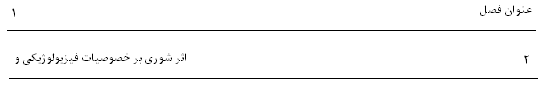
\includegraphics[width=.6\textwidth]{pages.png}
\caption{نمونه‌ای از شیوه‌ی صحیح قرارگیری مشخصات سرصفحه.}
\label{fig:header}
\end{figure}
			\begin{enumerate}[label=\Alph*:]
				\item سرصفحه (\lr{Header}) از صفحه‌ی دوم فصل اول شروع میشود و در صفحه‌ی اول هر فصل، قسمت سرصفحه حذف می‌شود. اول هر فصل باید \lr{break section} در بخش \lr{Page layout} استفاده شود تا سر فصل حذف شود و برای تکرار نشدن سرفصل‌ها در فصل‌های قبلی باید \lr{Link to previous} در بخش \lr{Design} استفاده شود.
				\item متن سرصفحه و شماره‌ی صفحه با قلم  \lr{BNazanin 12 Bold} نوشته شود. 
				\item صفحات سفید، سرصفحه ندارند. 
				\item صفحه‌ی اول فصل، پیوست، نمایه‌ها و واژه‌نامه، سرصفحه ندارند. 
				\item از صفحه‌ی فهرست تا شروع فصل اول، تمامی صفحات با حروف الفبای فارسی و در بالای صفحه، گوشه‌ی خارجی صفحه و به فاصله‌ی 5 سانتی‌متر از بالای كاغذ شماره‌گذاری ‌شود.
				\item از اولین صفحه‌ی فصل اول تا انتهای منابع، تمامی صفحات با اعداد1، 2، 3، و ... در بالای صفحه، گوشه‌ی خارجی صفحه و به فاصله‌ی 5 سانتی‌متر از بالای كاغذ شماره‌گذاری ‌شود.
			\end{enumerate}
			
		\section{نحوه‌ی نگارش}
			نرم‌افزار مورد استفاده برای نگارش پایان‌نامه،  \lr{Microsoft Word 2003} به بالا یا نرم‌افزار مناسب دیگر به تأیید كمیته‌ی تحصیلات تكمیلی دانشکده مربوطه می‌باشد. در صورت استفاده از برنامه \lr{Word}، توجه به نكات زیر ضروری است:  
			\begin{enumerate}%[label=\Alph*:]
				\item متن چکیده‌ی فارسی با قلم \lr{BNazanin 12} و کلمه «چکیده» در اولین خط با قلم \lr{BNazanin 12 Bold} در اول سطر درج شود. 
				\item متن چکیده‌ی انگلیسی با قلم \lr{Times New Roman 11} و کلمه \lr{Abstract} در اولین خط با قلم \lr{Time New Roman 11 Bold} در اول سطر درج شود. 
				\item متن مقدمه با قلم \lr{BNazanin 12} و کلمه «مقدمه» در اولین خط با قلم \lr{Bold  BNazanin 14} در اول سطر درج شود.
				\item متن اصلی پایان‌نامه باید روی دو طرف کاغذ \lr{A4} با قلم \lr{BNazanin 12} و با فاصله خطوط یکسان به صورت (\lr{Single}) نوشته شود. 
				\item در متن اصلی پایان‌نامه، لغات یا حروف انگلیسی (از جمله، منابع انگلیسی) با قلم \lr{Times New Roman 11} نوشته شود.
				\item عناوین فصل‌ها با قلم \lr{14 BNazanin Bold} نوشته شود.
				\item سطر اول تمامی پاراگراف‌های موجود در متن پایان‌نامه، بایستی $0.5$ سانتی‌متر تورفتگی داشته باشند. توجه داشته باشید که عنوان بخش‌ها یا زیر بخش‌ها نبایستی دارای تورفتگی باشند.
				\item قسمت‌های مختلف هر فصل با اعدادی نظیر 6-4- یا 6-4-2- مشخص میشود كه عدد 6 شماره‌ی فصل، عدد4 شماره‌ی بخش و عدد 2 شماره‌ی زیر بخش است. بخش‌های مختلف فصل‌ها با قلم \lr{BNazanin 13 Bold} و زیربخش‌های اول با قلم \lr{BNazanin 12 Bold}  و زیربخش‌های دوم با \lr{BNazanin 11 Bold} تایپ شود.
				\item تمامی شکل‌ها و جدول‌ها باید به ترتیب ظهور در هر فصل شماره‌گذاری شوند. مثلاً برای جدول‌های فصل 2، جدول 2-1، جدول 2-2 و ... برای جدول‌های فصل 3، جدول 3-1، جدول 3-2 و .... عنوان جدول‌ها در بالای آن‌ها و وسط صفحه و عنوان شکل‌ها در زیر آنها، وسط صفحه با قلم \lr{BNazanin 10 Bold}  نوشته شود. اعداد و متن داخل جدول با قلم \lr{BNazanin 10}   نوشته شود. اگر شکلی از مرجعی نقل شده باشد، لازم است مرجع آن در زیر شکل داخل پرانتز آورده شود.
				\item جدول‌هایی که در راستای طولی کاغذ تنظیم میشوند، باید طوری قرار گیرند که متن بالای آنها در سمت لبه‌ی پایان‌نامه واقع شود (درتمامی جدول‌ها خطوط عمودی باید حذف شود). شکل‌ها و جدول‌ها داخل متن و در نزدیکترین فاصله به محل ذکر شده، آورده شوند (حاشیه‌ی شکل‌ها حذف شود). هم‌چنین شکل‌هایی که در راستای طولی کاغذ تنظیم می‌شوند، باید طوری قرار گیرند که متن پایین آنها در سمت لبه‌ی پایان‌نامه قرار گیرد. 
				\item فرمول‌ها (در صورت نیاز به ارجاع) در هر فصل به‌طور جداگانه و به ترتیبی که ظاهر می‌شوند (مانند جدول‌ها و شکل‌ها) شماره‌گذاری می‌گردد (مانند 2-3، 2-4، 3-1 و ...).
				\item معادل انگلیسی لغات یا اصطلاحات فارسی که برای اولین‌بار به کار می‌رود به صورت زیرنویس (فقط برای یک‌بار) با قلم Times New Roman 10 در صفحه‌ی مربوط درج شود. (سعی شود در متن پایان‌نامه‌، از بکار بردن واژه‌های با الفبای انگلیسی خودداری شود). زیرنویس‌ها در هر صفحه با گذاردن شماره‌ی 1، 2 و ... در گوشه‌ی بالای آخرین کلمه در متن مشخص میشوند. زیر نویس باید به شکل زیر در زیر نویس آورده شود. \\
\begin{latin}
\footnotesize	$1$ Water use efficiency
\end{latin}
				\item لازم است در متن به تمامی منابعی كه مورد استفاده قرار می‌گیرند، اشاره شود. چنانچه در داخل متن از یك منبع مطلبی نقل شود، بلافاصله پس از ذكر نام نویسنده و یا در خاتمه‌ی جمله، پرانتزی باز شود و مرجع ذكر گردد. شیوه‌ی نامه‌ی نگارش منابع پیوست شده است (پیوست شماره‌ی \ref{app6}).
				
			\end{enumerate}

		حاشیه‌های صفحات مطابق نمونه‌ی شکل \ref{layout} ($4.5$ سانتیمتر فاصله از بالا و پایین و $4$ سانتیمتر از چپ و $5$ سانتیمتر از راست رعایت گردد (توجه: برای تنظیم این فاصله‌ها از حاشیه از طریق \lr{Page layout} وارد \lr{Page setup} شده و اعداد را با واحد سانتیمتر وارد کنید. در ضمن در همان صفحه در قسمت \lr{Multiple pages} کلمه \lr{mirror margin} را انتخاب کنید تا در صفحات زوج و فرد فاصله متن از حاشیه بیرونی $4$ سانتیمتر و از حاشیه درونی $5$ سانتیمتر شود (در \lr{Page setup} باید سایز (\lr{Size Letter}) انتخاب شود).
		
		\begin{figure}
	\centering
	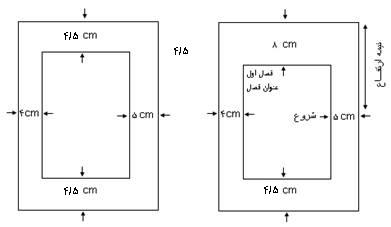
\includegraphics[width=.6\textwidth]{layout.png}
\caption{حاشیه‌ی صفحات.}
\label{layout}
\end{figure}
\section{نحوه‌ی صحافی پایان‌نامه}
	روی جلد مطابق یا پیوست شماره‌ی \ref{app1} تنظیم گردد، عطف آن مانند نمونه‌ی شکل \ref{atf} نوشته می‌شود.
	\begin{figure}
	\centering
	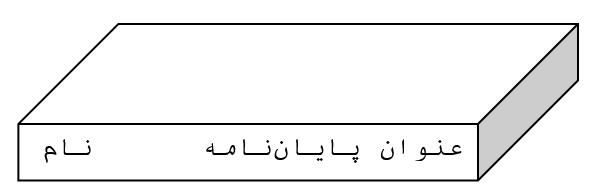
\includegraphics[width=.6\textwidth]{atf.png}
\caption{نمونه‌ای از شیوه‌ی صحیح \gls*{typeset} عطف.}
\label{atf}
\end{figure}
ابعاد پایان نامه بعد از صحافی، $23.5 \times 17$ (قطع وزیری) باید باشد. ابعاد سیاهه متن پایان‌نامه (از بالای متن سرصفحه تا پایین متن اصلی و عرض متن) $18.3 \times 12$ باید باشد. 
فاصله‌ی متن سرصفحه از حاشیه‌ی بالا $2.5$ سانتیمتر و فاصله‌ی متن اصلی از حاشیه‌ی پایین $2.7$ سانتیمتر، فاصله‌ی متن از حاشیه‌ی بیرونی $2$ سانتیمتر و از حاشیه‌ی درونی $3$ سانتیمتر باید باشد.  

رنگ جلد پایان‌نامه‌های کارشناسی‌ارشد کلیه رشته‌ها سورمه‌ای و رساله دکتری سبز یشمی می‌باشد. همچنین، اصل پایان‌نامه قبل از صحافی و پس از تایپ و آماده‌سازی به رؤیت مدیر تحصیلات تكمیلی دانشگاه یا معاون آموزشی دانشكده رسانیده شود و پس از مطابقت با ضوابط مصوب، تأییدیه صادر گردد.


	\chapter{نتیجه‌گیری}
در این فصل، نتیجه‌گیری پایان‌نامه‌ی خود را درج کنید.
			
	\appendix
	\chapter{یک پیوست}
مطالب این پیوست بر اساس راهنمای نگارش پایان‌نامه‌های تحصیلات تکمیلی در \cite{vru_grad_rules} تهیه شده‌اند. 

	\begin{figure}
		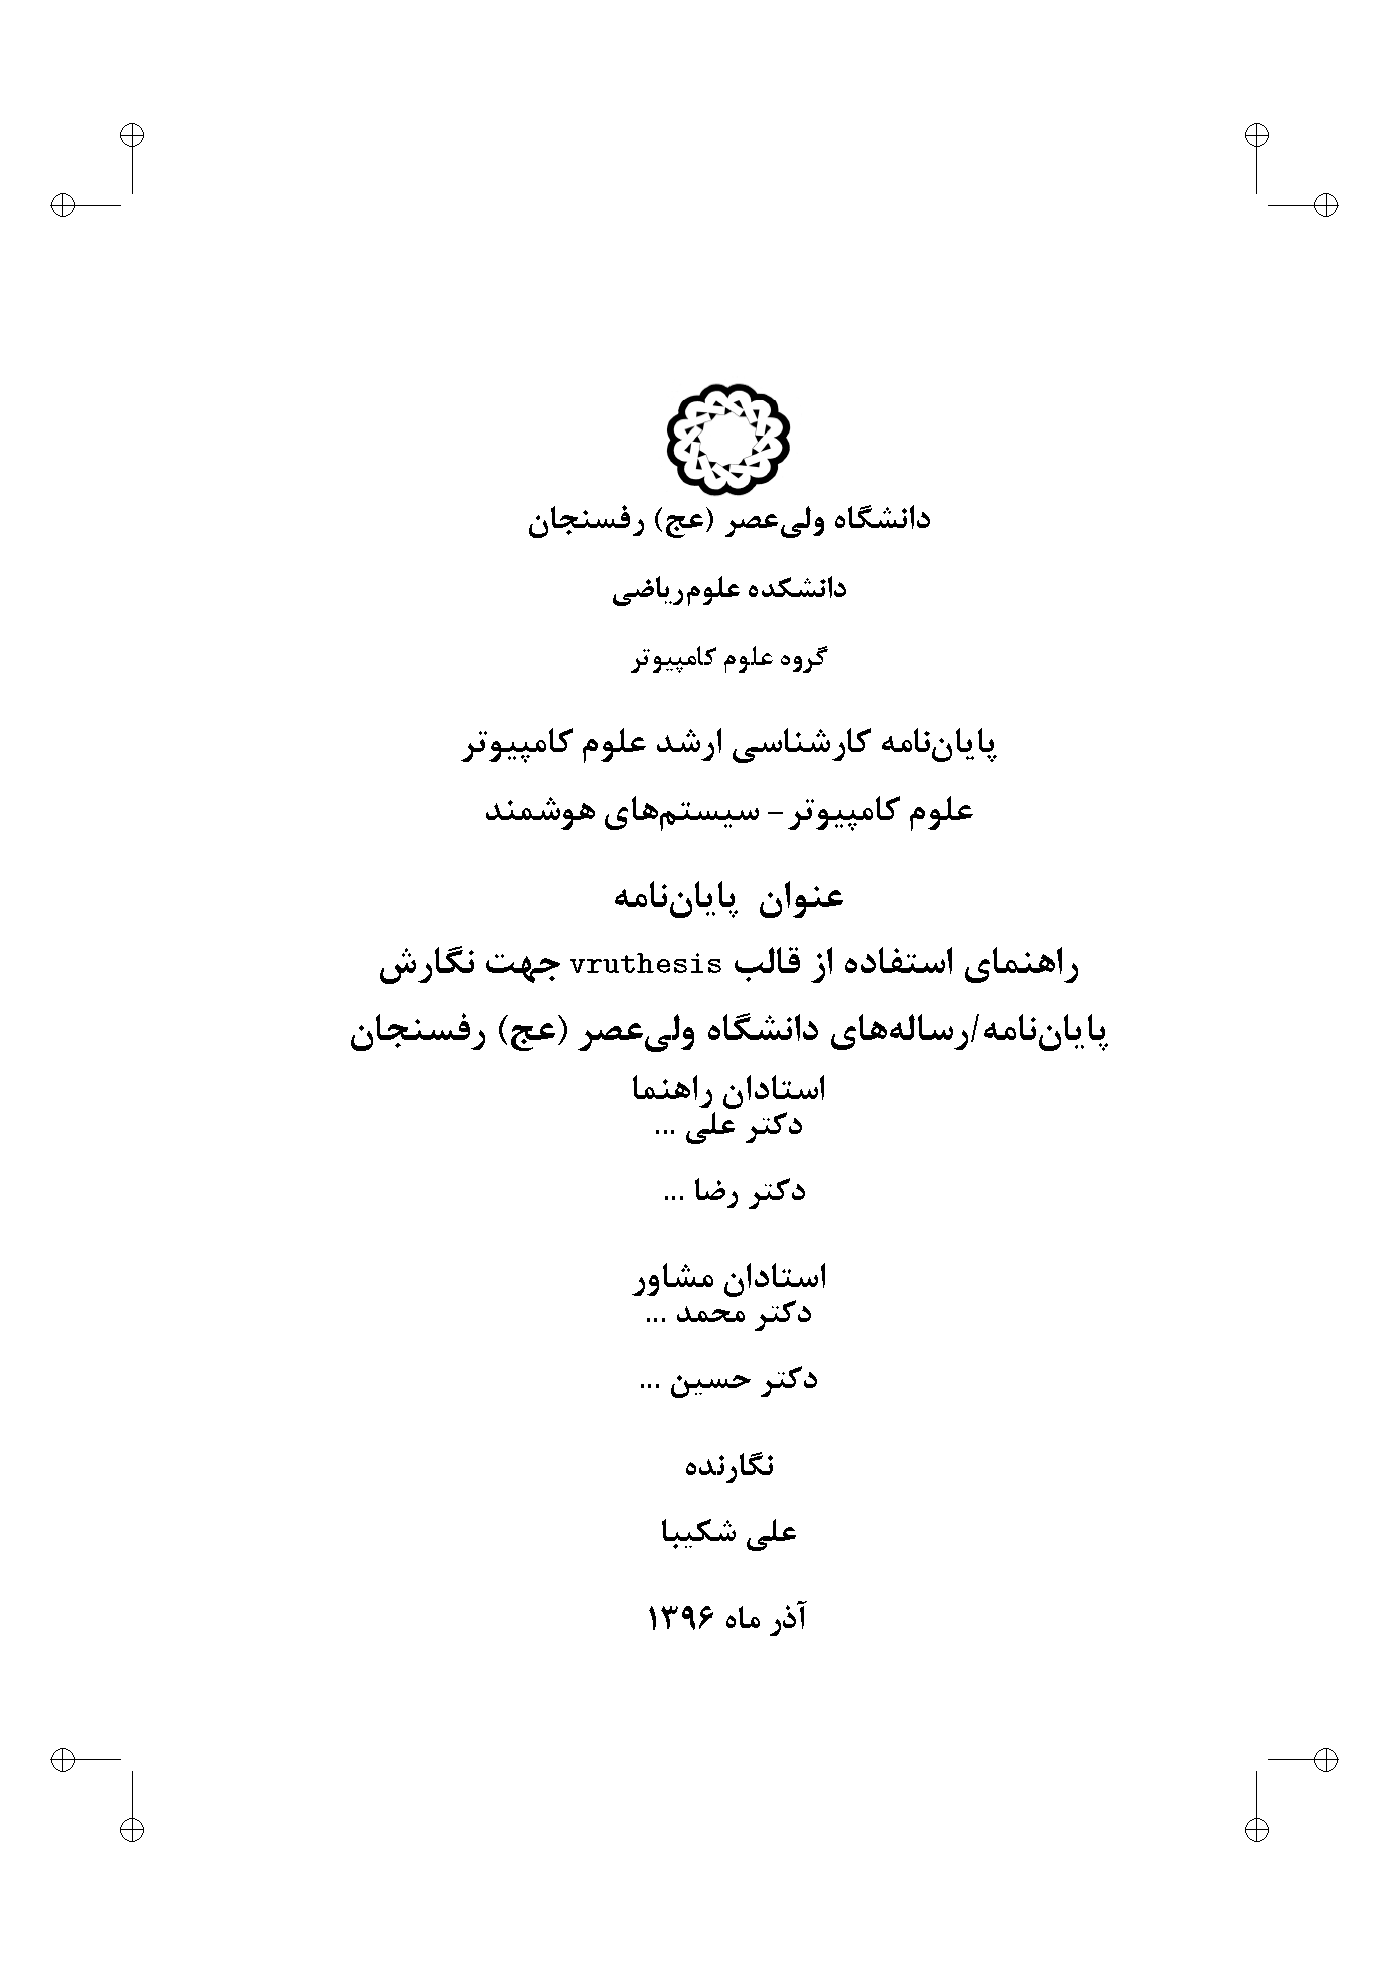
\includegraphics[width=\textwidth]{a.png}
		\caption{نمونه‌ی صفحه‌ی اول پایان‌نامه‌ی کارشناسی ارشد.}
		\label{app1}
	\end{figure}

	\begin{figure}
		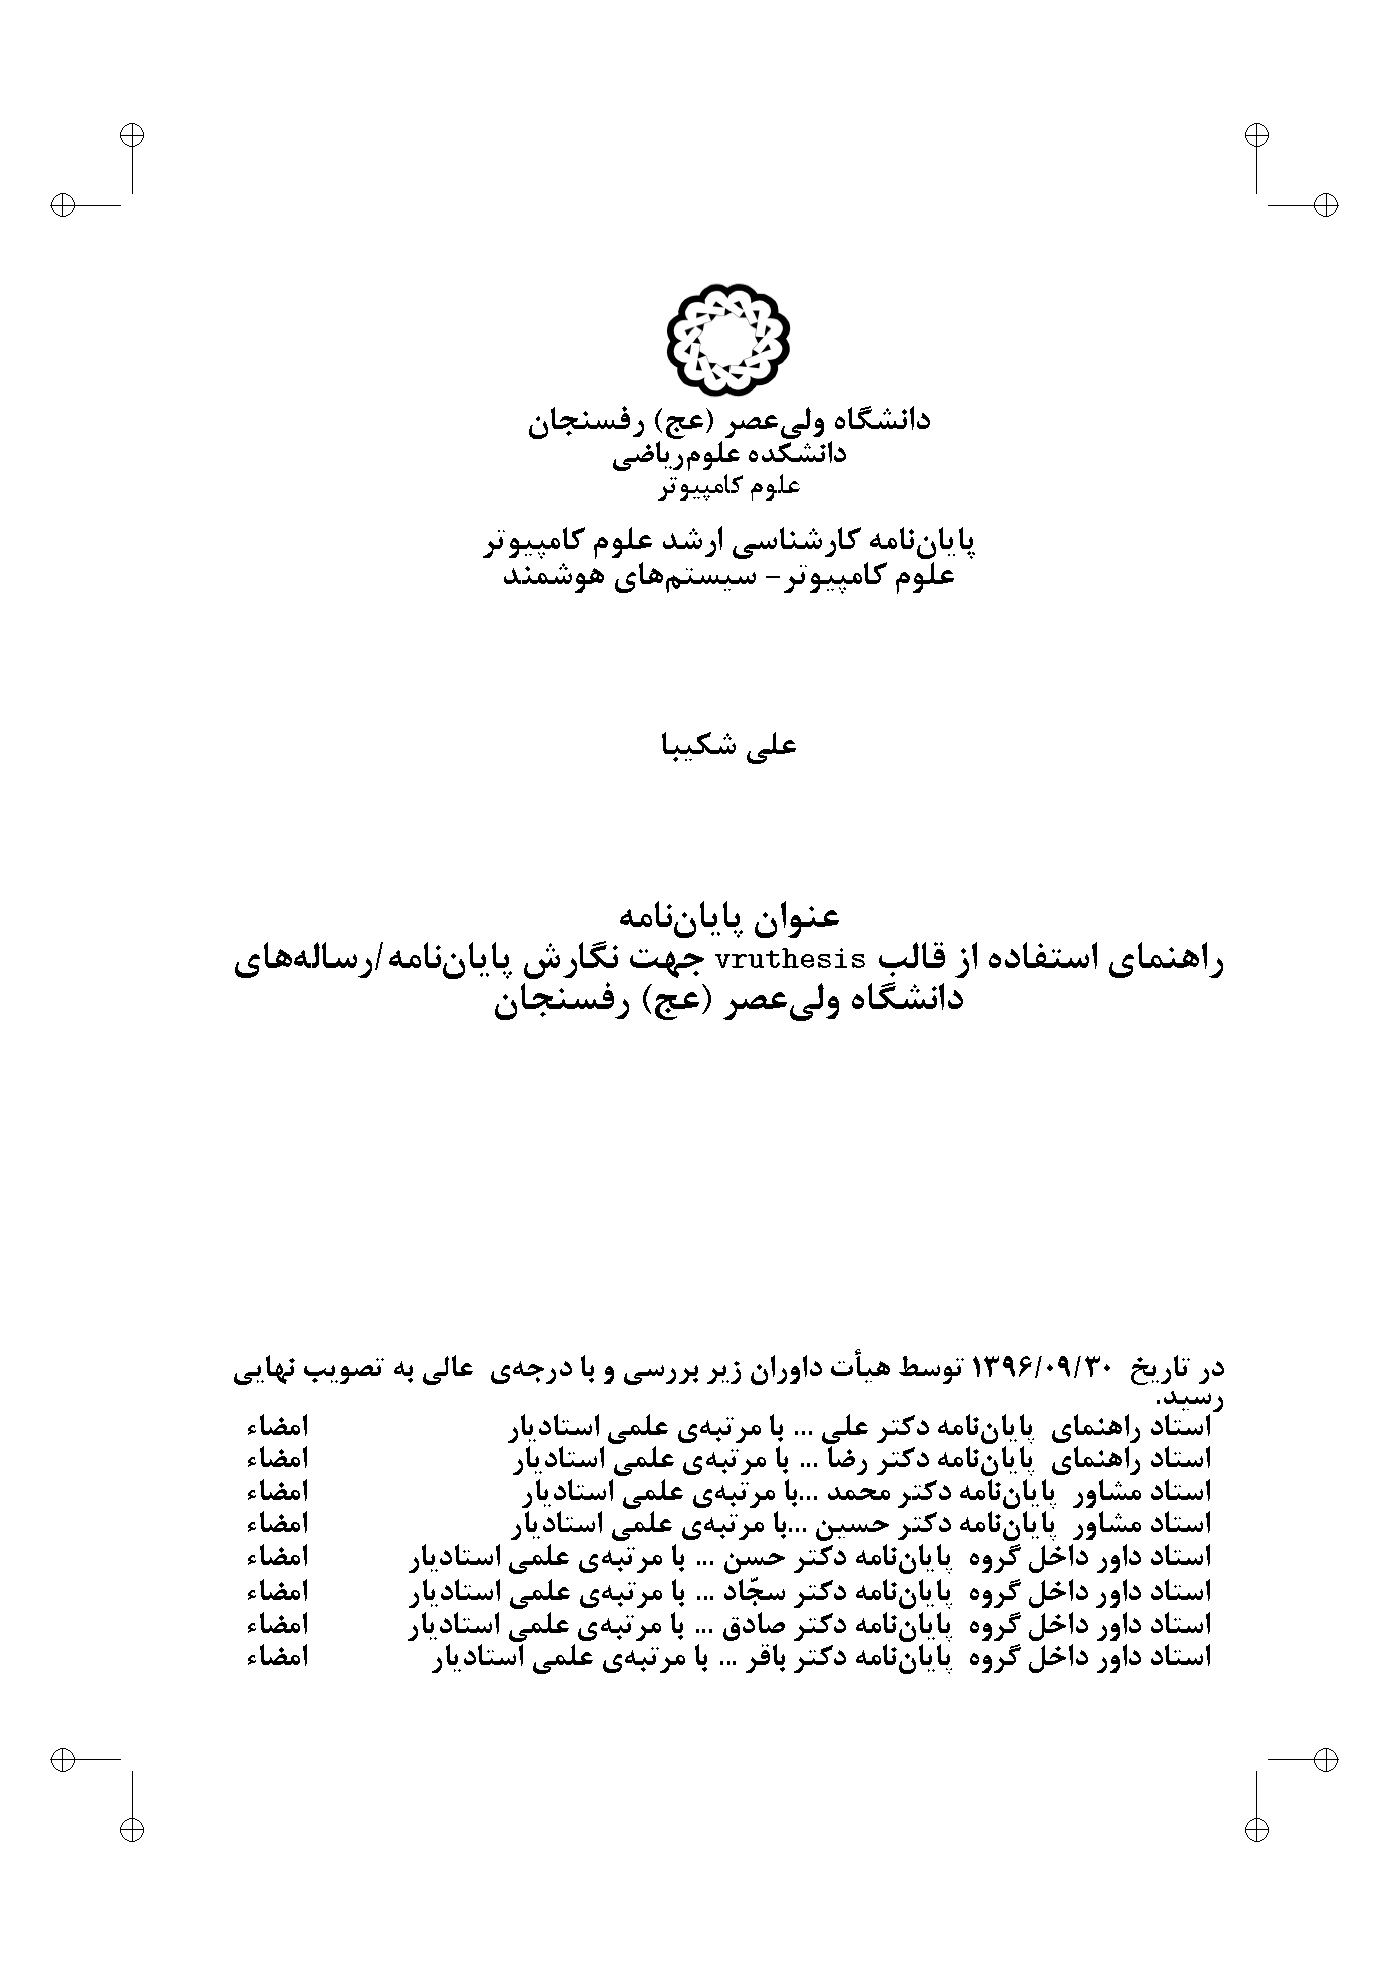
\includegraphics[width=\textwidth]{b.png}
		\caption{نمونه‌ی تصویب‌نامه‌ی پایان‌نامه‌ی کارشناسی ارشد.}
		\label{app2}
	\end{figure}

	\begin{figure}
		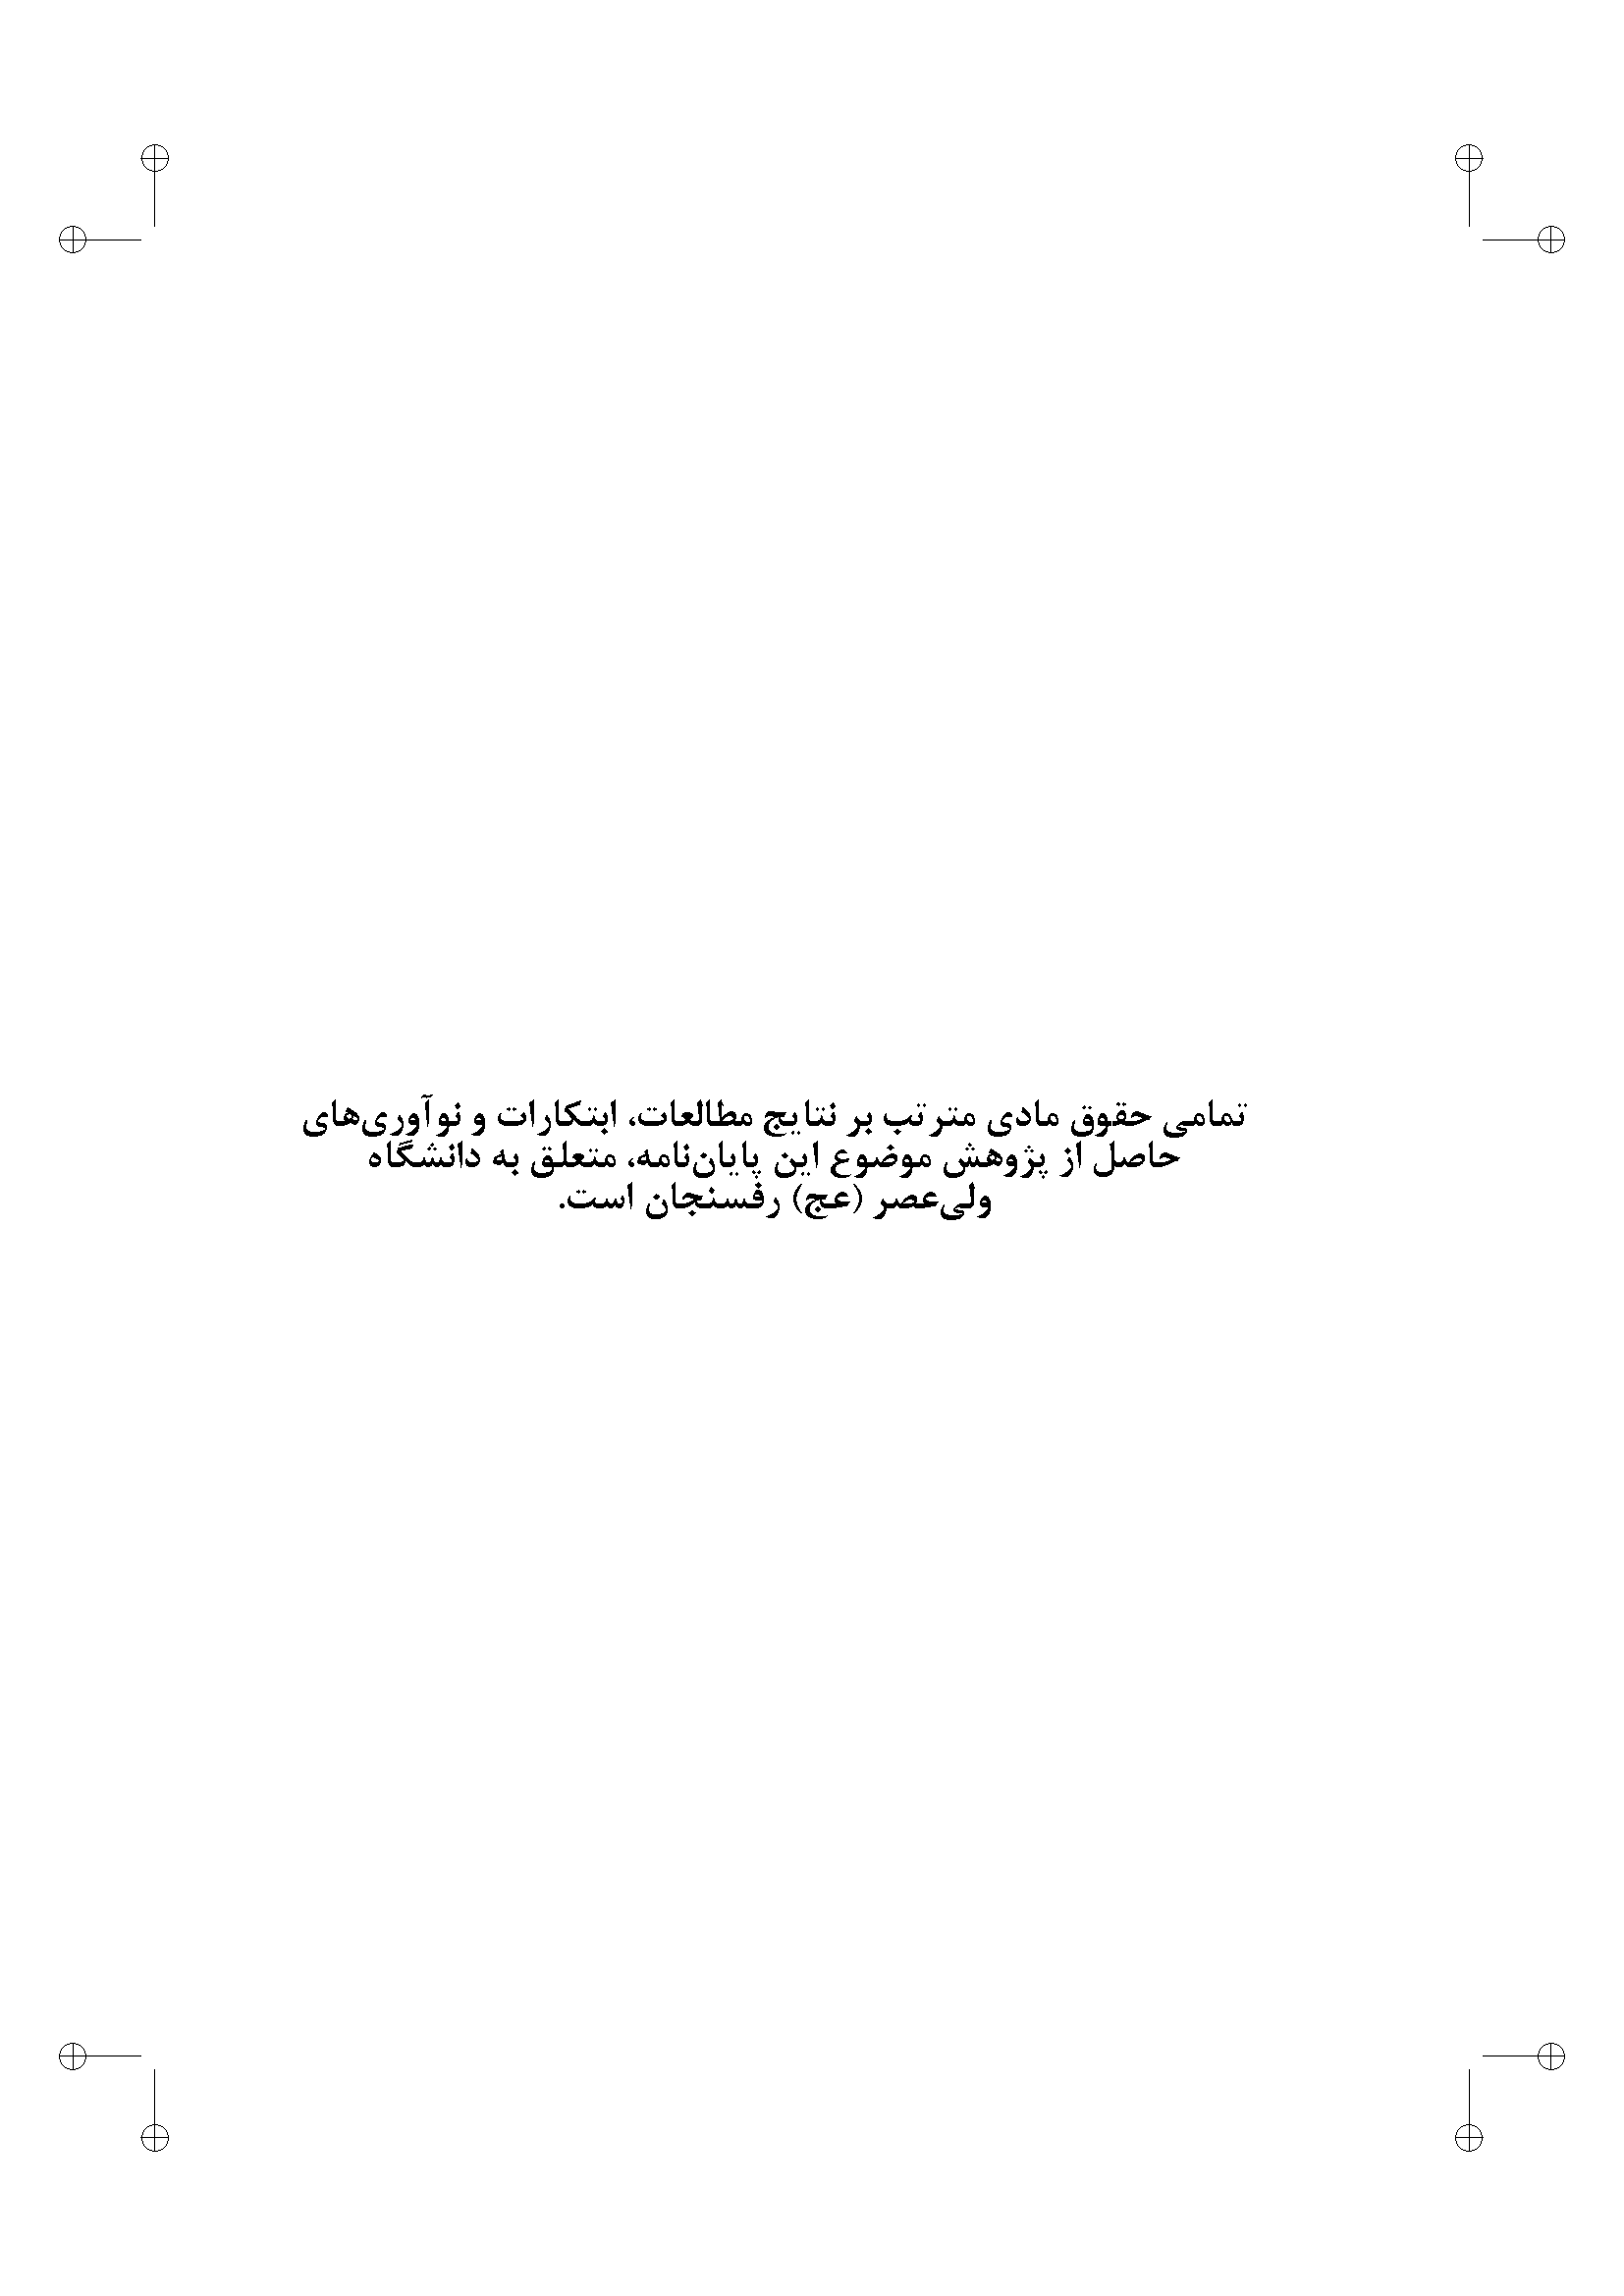
\includegraphics[width=\textwidth]{d.png}
		\caption{تعهدات حقوقی.}
		\label{app4}
	\end{figure}

	\begin{figure}
		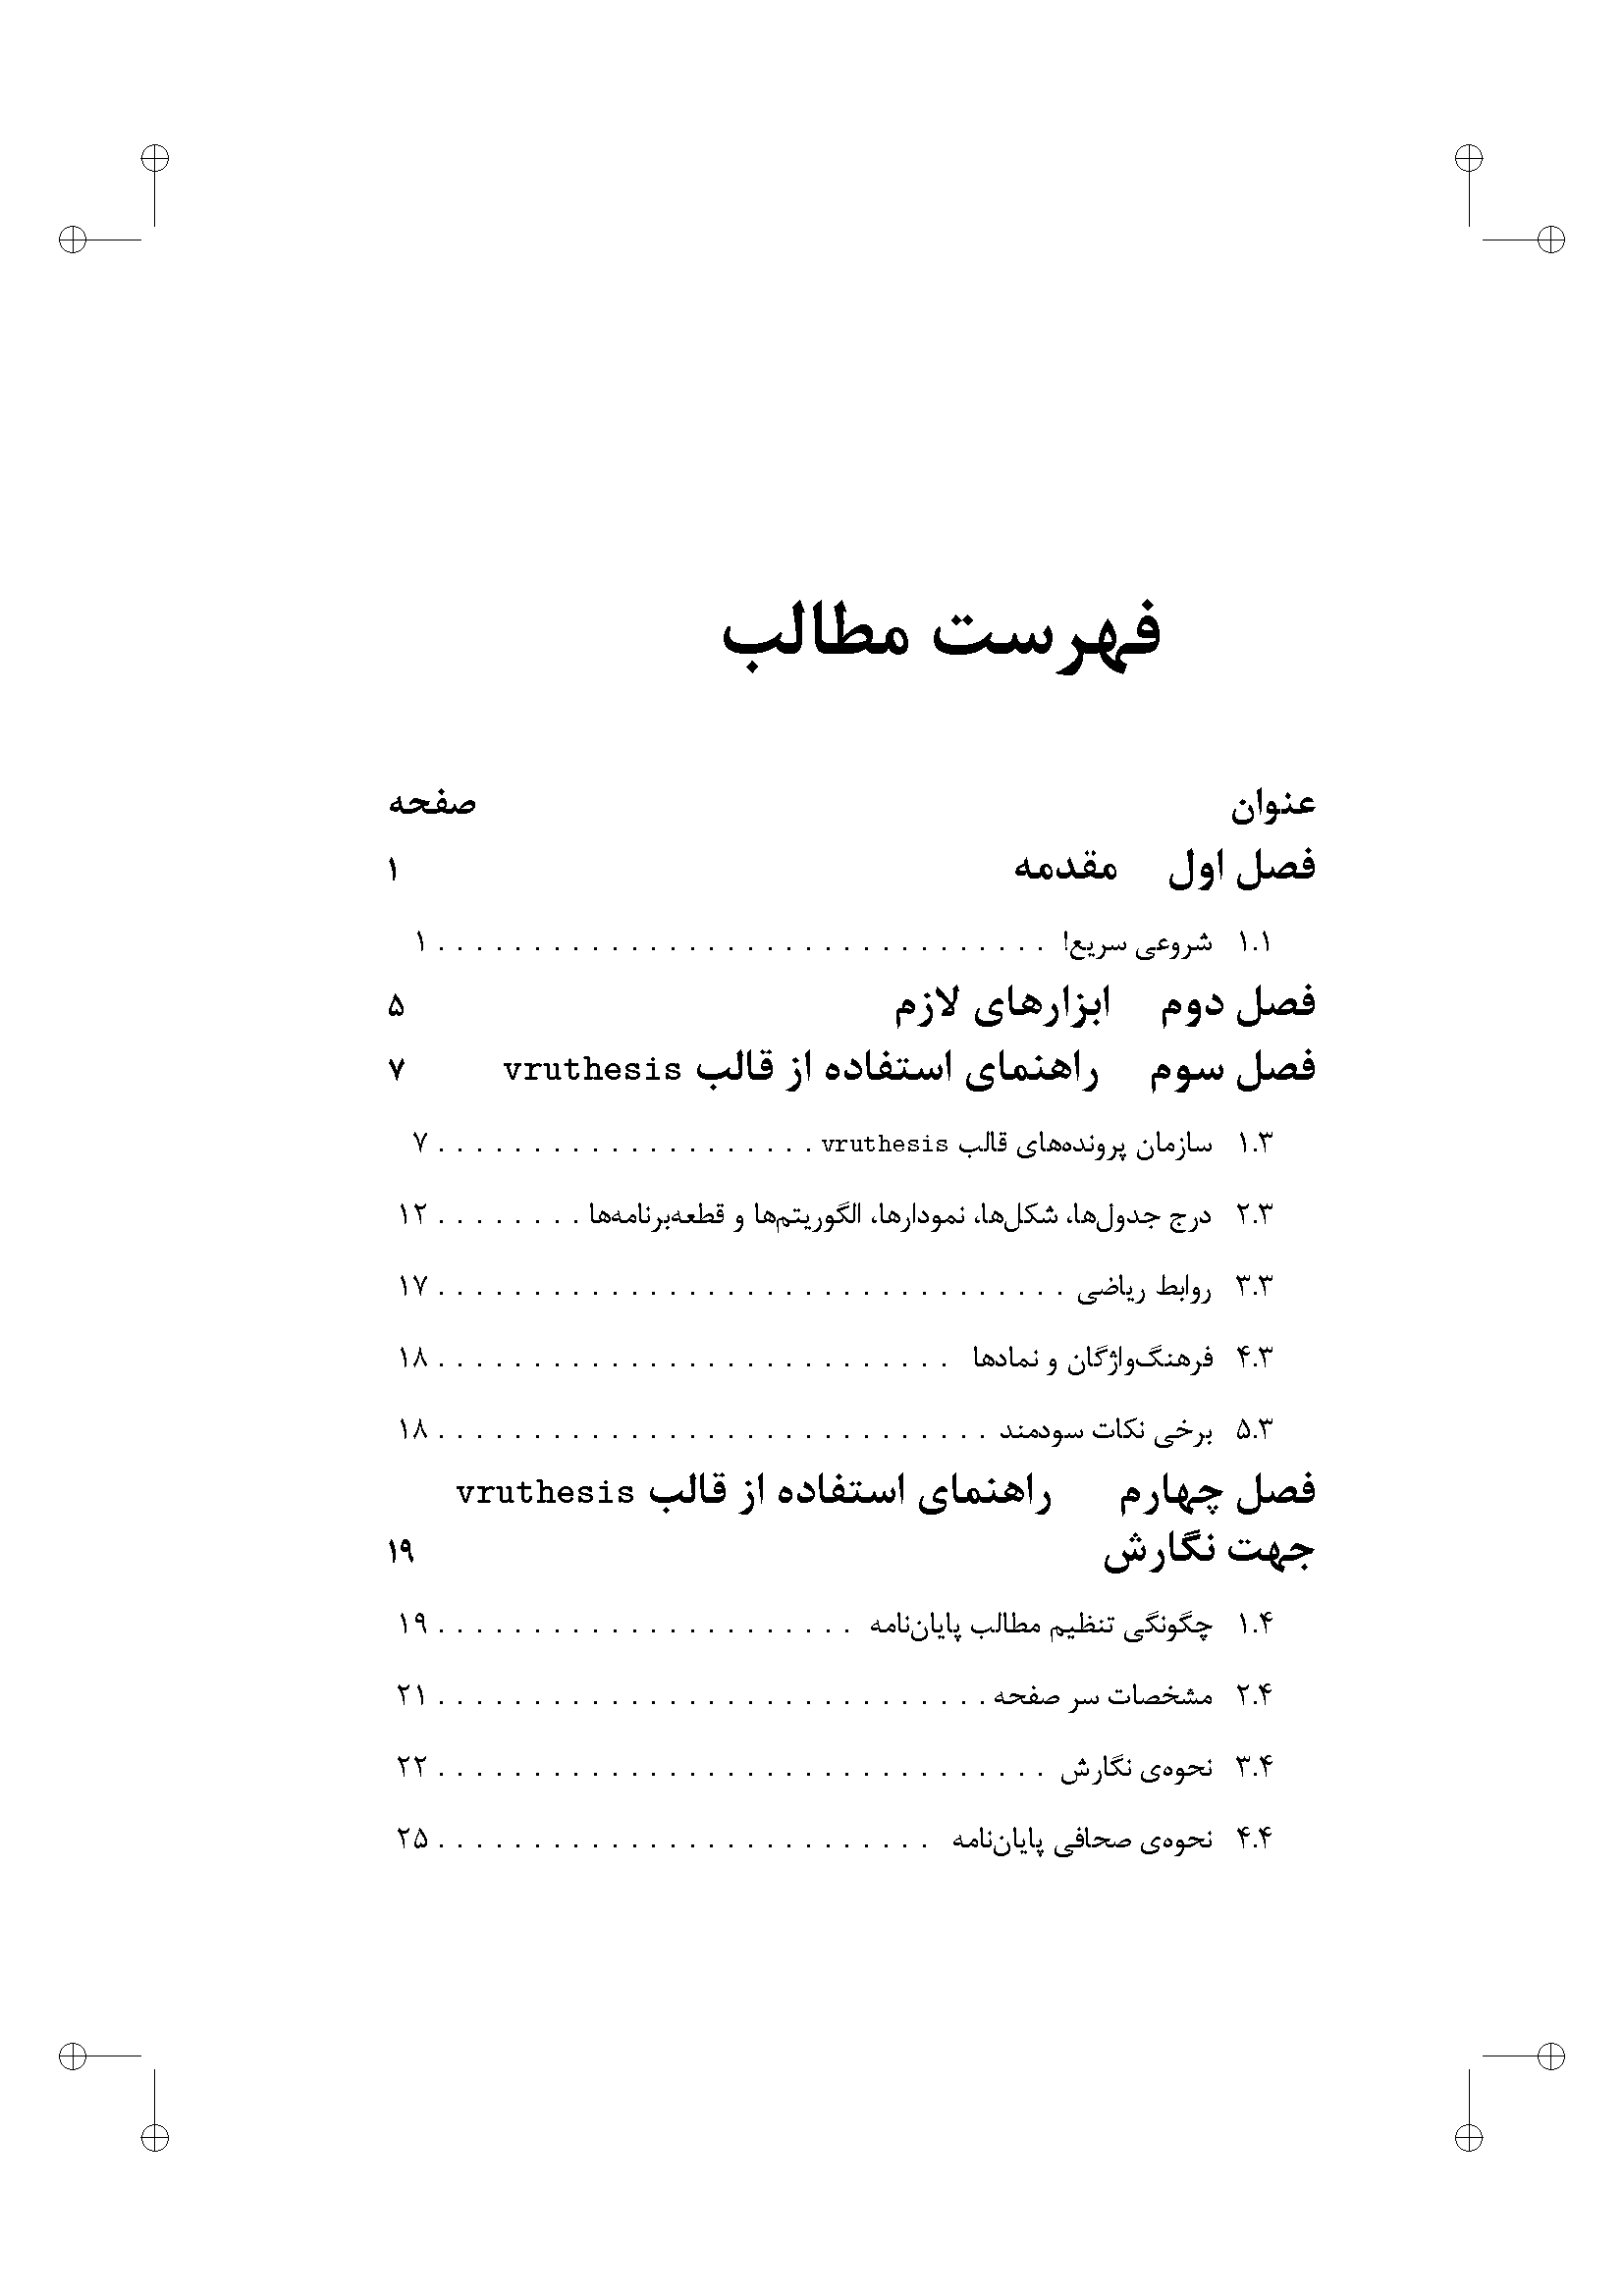
\includegraphics[width=\textwidth]{e.png}
		\caption{نمونه‌ای از فهرست مطالب.}
		\label{app5}
	\end{figure}

	\begin{figure}
		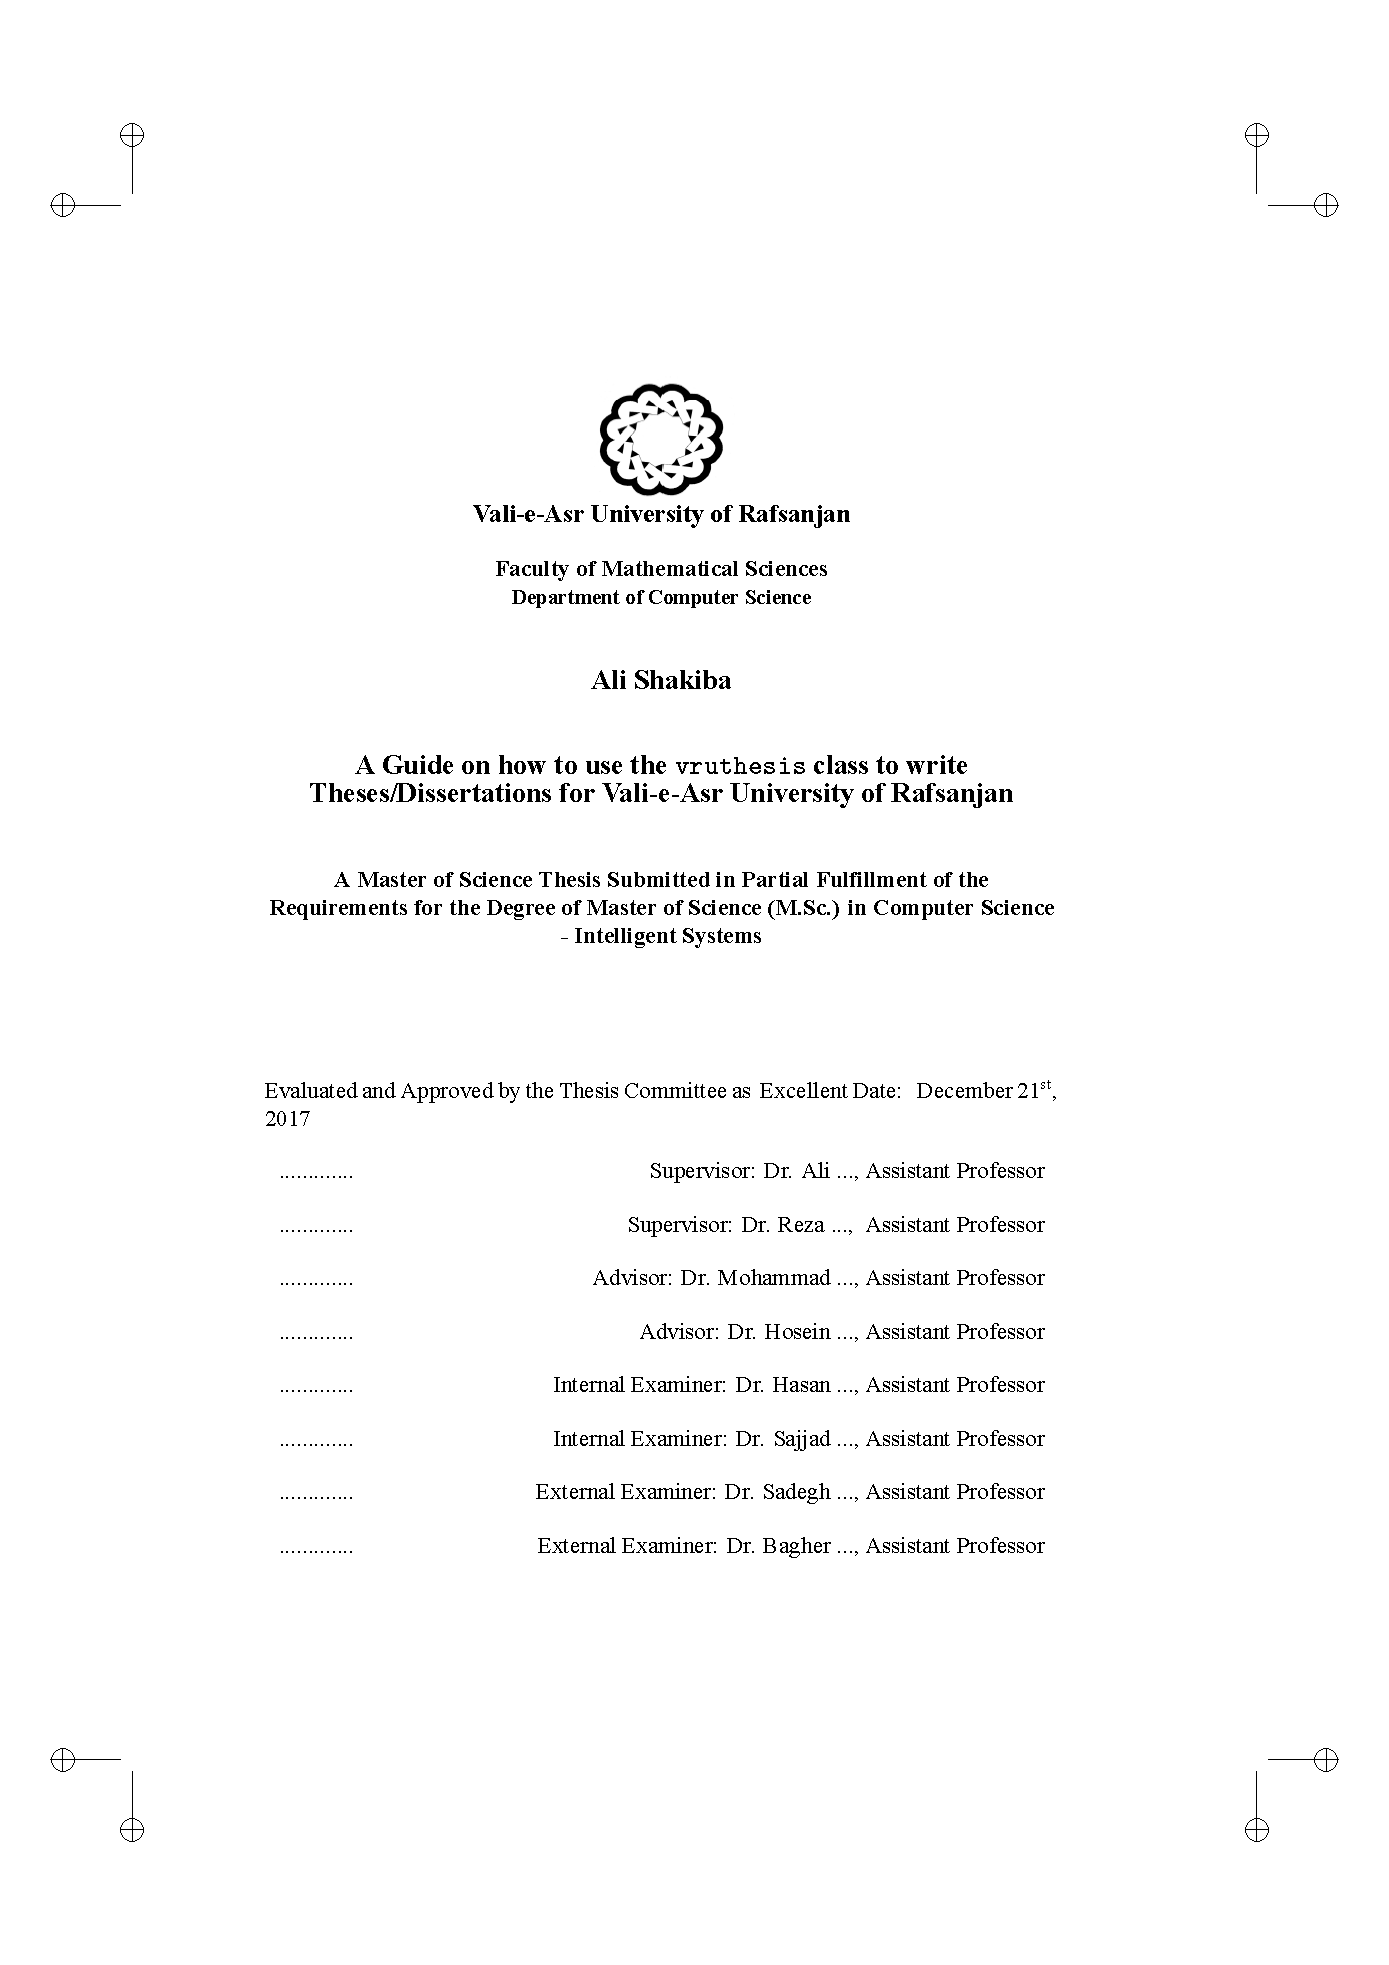
\includegraphics[width=\textwidth]{c.png}
		\caption{نمونه‌ی تصویب‌نامه‌ی پایان‌نامه‌ی کارشناسی ارشد به زبان انگلیسی.}
		\label{app3}
	\end{figure}

	\begin{figure}
		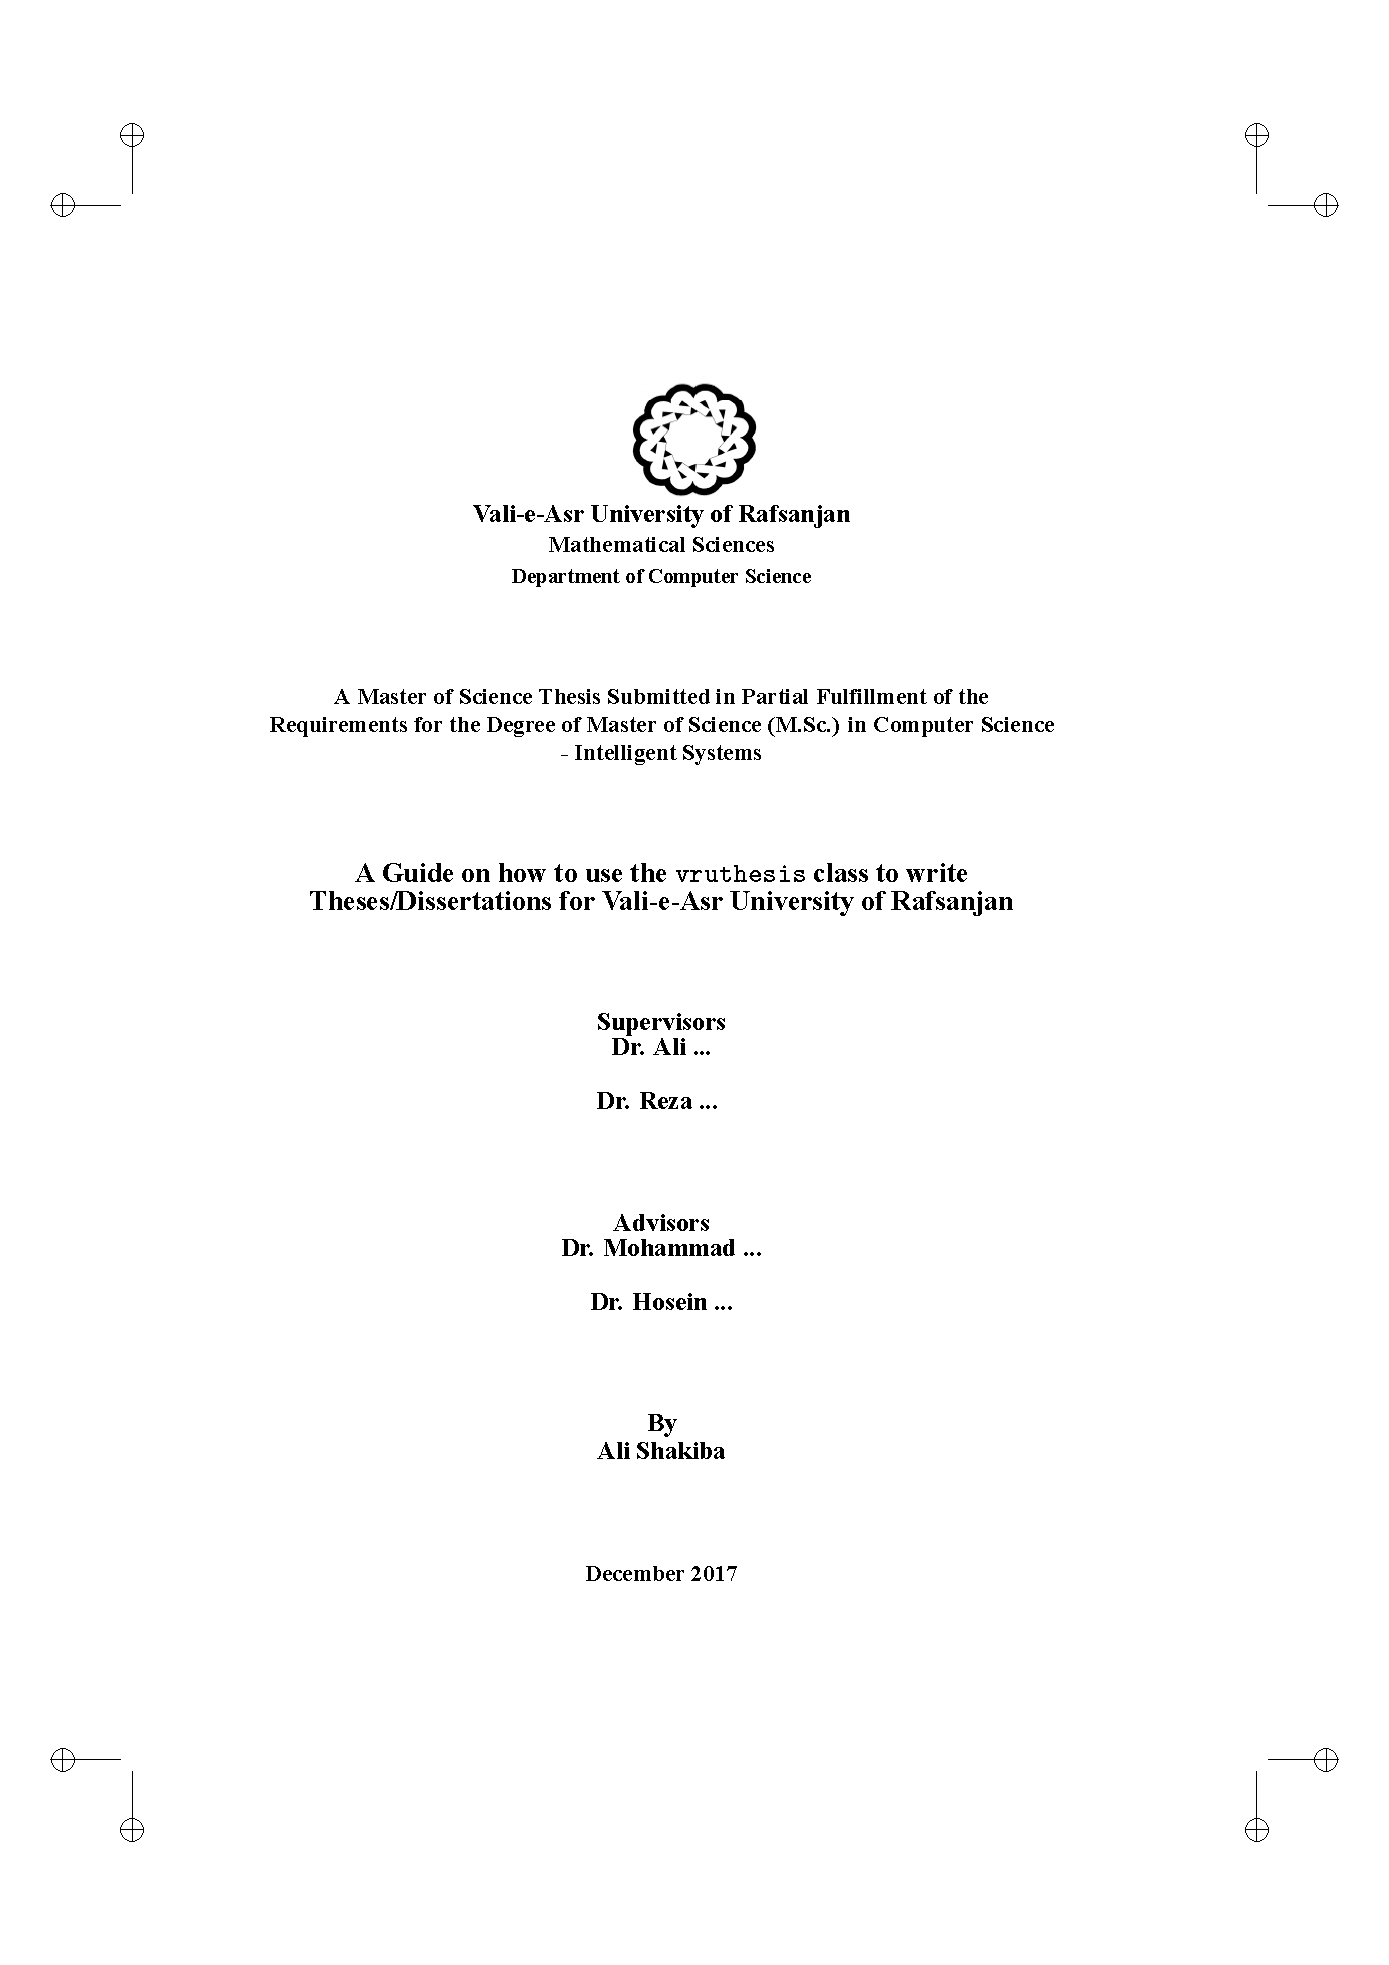
\includegraphics[width=\textwidth]{f.png}
		\caption{نمونه‌ی صفحه‌ی آخر پایان‌نامه‌ی کارشناسی ارشد.}
		\label{app6}
	\end{figure}

% +rl|از این قسمت به بعد را به هیچ وجه تغییر ندهید.$
	% لطفا هیچ تغییری در این فایل صورت ندهید.
	\cleardoublepage
	\printglossary
	\cleardoublepage
	\cleardoublepage
	\addcontentsline{toc}{chapter}{فهرست مراجع}
	\bibliography{references}
	\vrutitleen
\end{document}
		\end{mynewverbatim}
		\caption{محتویات \gls*{file} \lr{\texttt{thesis.tex}} نمونه.}
		\label{fig:ch1:thesis}
	\end{figure}
	این \gls{file} برای \gls{typeset} پایان‌نامه‌های کارشناسی ارشد دانشکده‌ی ریاضی در قطع وزیری، با چاپ دورو آماده شده است. همچنین، به منظور سهولت در فرایند صحافی، خطوط راهنما جهت برش کاغذ، در هر صفحه نمایش داده شده اند. 
	
		قواعد زیر؛ تنها قواعدی هستند که برای \gls{typeset} پایان‌نامه‌ی خود، نیاز است تا بدانید:
	\begin{itemize}
		\item اطلاعات مورد نیاز برای تولید صفحات ابتدایی و انتهایی پایان‌نامه، مانند چکیده‌، تقدیم‌به و مانند آن، در \gls{file} \lr{\texttt{data.tex}} قرار دارند. 
		\item مطالب هر یک از فصل‌ها را در یکی از \glspl{file}ی \lr{\texttt{chapterX.tex}} قرار دهید.
		\item پیوست‌ها در  \glspl{file}ی \lr{\texttt{appendixX.tex}} قرار می‌گیرند.
		\item قالب تولید فهرست مراجع در خط $10$ تعیین می‌گردد. برای تولید موفقیت آمیز فهرست مراجع، وجود \gls{file} \lr{\texttt{BibStyle.bst}} که \lr{\texttt{BibStyle}} بیانگر قالب مورد استفاده است؛ الزامی است.
		\item اطلاعات مربوط به مراجع در \gls{file} \lr{\texttt{references.bib}} به صورت \lr{bibtex} قرار می‌گیرند.
		\item واژگان در \gls{file} \lr{\texttt{gloss.tex}} و اختصارات و نمادها در \gls{file} \lr{\texttt{acronym.tex}} تعریف می‌شوند.
		\item دستورات لازم برای تولید خروجی در شکل \ref{fig:ch1:output_cmd} آمده‌اند. 
		\item وجود \glspl{file}ی \lr{\texttt{vruthesis.cls}}، \lr{\texttt{settings.tex}}، \lr{\texttt{data.tex}}، و \lr{\texttt{finalpart.tex}} جهت تولید خروجی موفق، الزامی است.
		\item در صورت نیاز برای \gls{typeset} رساله‌ی دکتری، در خط اول \gls{file} \lr{\texttt{chapterX.tex}}، کلمه‌ی \lr{phd} را به ویژگی‌ها اضافه نمایید.
		\item در صورتی که پایان‌نامه‌ی شما فاقد الگوریتم است؛ فهرست الگوریتم‌ها را با برداشتن کلمه‌ی \lr{alg} از ویژگی‌های خط اول \gls{file} \lr{\texttt{chapterX.tex}}، غیر فعال نمایید.
	\end{itemize}
				\begin{figure}
		\begin{latin}
\centering
	\begin{verbatim}
	xelatex -synctex=-1 thesis.tex
bibtex8 -W -c cp1256fa thesis
xindy -L persian-variant1 -C utf8 -I xindy -M thesis.xdy 
        -t thesis.glg -o thesis.gls thesis.glo
xindy -L persian-variant1 -C utf8 -I xindy -M thesis.xdy 
        -t thesis.blg -o thesis.bls thesis.blo
xindy -L english -C utf8 -I xindy -M thesis.xdy -t thesis.alg 
        -o thesis.acr thesis.acn
xelatex -synctex=-1 thesis.tex
xelatex -synctex=-1 thesis.tex
	\end{verbatim}
	\end{latin}
\caption{دستورات لازم برای تولید خروجی نهایی به قالب \gls*{pdf}.}
\label{fig:ch1:output_cmd}
\end{figure}
\section{یک بخش آزمایشی}
در این قسمت، نمونه‌ای از بخش‌بندی‌های ممکن نمایش داده می‌شوند.
	\subsection{یک زیربخش}
	زیربخش‌ها می‌توانند در صورت لزوم دارای زیرزیربخش باشند.
		\subsubsection{یک زیرزیربخش}
		لطفا توجه داشته باشید که بخش‌بندی بیش از چهار سطح، مجاز نیست.
\newpage
این متن جهت آزمودن تعداد خطوط در هر صفحه از ویکی‌پدیای فارسی درباره‌ی خوارزمی برداشته شده است. 
محمد بن موسی خوارزمی (زاده حدود سال ۷۸۰ میلادی و درگذشته ۸۵۰ میلادی) ریاضیدان، ستاره‌شناس، فیلسوف، جغرافیدان و مورخ شهیر ایرانی[۲] در دوره عباسیان است. وی در حدود سال ۷۸۰ میلادی (قبل از ۱۸۵ قمری)[۱] در خوارزم زاده شد. ابن ندیم و قفطی اصالت او را از خوارزم می‌دانند. لقب وی معمولاً اشاره به شهر خوارزم دارد که همان خیوه کنونی واقع در جنوب دریاچه آرال مرکزی و بخشی از جمهوری ازبکستان کنونی است.[۱] شهرت علمی وی مربوط به کارهایی است که در ریاضیات، به‌ویژه در رشته جبر، انجام داده به‌طوری‌که هیچ‌یک از ریاضیدانان سده‌های میانه مانند وی در فکر ریاضی تأثیر نداشته‌اند و وی را «پدر جبر» نامیده‌اند.[۳] جرج سارتن، مورخ مشهور علم، در طبقه‌بندی سده‌ای کتاب خود مقدمه‌ای بر تاریخ علم سده نهم میلادی را «عصر خوارزمی» می‌نامد.[۴][۵]

خوارزمی ریاضی‌دان بنام قرون وسطی است که حاصل تحقیقات و تألیفات او هنوز مورد استفاده می‌باشد و کتاب جبر و مقابله او را بسیاری از مترجمان مشهور قرون وسطی ترجمه کرده‌اند. بیشترین چیره‌دستی وی در حل معادله‌های خطی و درجه دوم بوده‌است. کتاب Algoritmi de numero Indorum که ترجمه کتاب جمع و تفریق با عددهای هندی او به لاتین است باعث شد تا دستگاه عددی در اروپا از عددنویسی رومی به عددنویسی هندی-عربی تغییر یابد؛ چیزی که هنوز نیز در اروپا و دیگر نقاط جهان فراگیر است.[۶] واژه جبر را اروپائیان بطور کلی از کتاب خوارزمی و اصطلاح امروزی الگوریتم (Algorithmus) از نام خوارزمی گرفته شده‌است. به هنگام خلافت مأمون، وی عضو دارالحکمه که مجمعی از دانشمندان در بغداد به سرپرستی مأمون بود، گردید. خوارزمی کارهای دیوفانت را در رشته جبر دنبال کرد و به بسط آن پرداخت.
گویند قبل از اینکه محمد بن موسی خوارزمی در دارالحکمه مستقر شود او را به سرزمین هند فرستادند تا حساب هندی را بیاموزد خوارزمی پس از بازگشت از هند دو اثر «حساب الهند» و دیگری «الجبر و المقابله» را نگاشت. وی نتایجی را که یونانیان و هندیان بدست آورده بودند را تلفیق کرد و بدین ترتیب سبب انتقال مجموعه‌ای از معلومات جبری حسابی شد که در ریاضیات قرون وسطی تأثیر عمیقی گذاشت.[۱۱]
محمد بن موسی خوارزمی در قرن سوم هجری، علمی را برای نخستین بار صورتبندی و تدوین کرد که خود آن را «الجبر و المقابله» نامید، علمی که تمام شرایط یک دانش واقعی را داشت، یعنی همان که اروپاییان از آن به «ساینس» تعبیر می‌کنند. این ریاضی‌دان توانست با این دانش تمام معادلات درجه دوم زمان خود راحل و راه را برای حل معادلات درجه بالاتر هموار کند.
ر اساس الواح بابلی و آثار برجای‌مانده از محاسبه‌گران هندی در عهد باستان، مردمان بابل و هند به حل حالات خاصی از معادلات درجه دوم موفق شده بودند، اما آن‌ها راه حل‌های خود را فقط به صورت دستور ارائه کردند؛ یعنی این راه حل‌ها، که برای رفع نیازهای زندگی روزمره آنان ارائه شده بودند و نه به منظور گسترش دانش ریاضی، فاقد براهین علمی بودند. ابتکار خوارزمی در آن است که وی نخست همه معادلات درجه دوم شناخته‌شده زمانش را بررسی می‌کند؛ در مرحله دوم روش حل هریک از آن‌ها را ارائه می‌دهد؛ سرانجام در مرحله سوم، این روش‌ها را با کمک علم هندسه اثبات می‌کند؛ مؤلفه‌هایی که درمجموع علم جدیدی به نام «جبر» را تشکیل می‌دهند. این علم، که از طریق ترجمه‌های لاتینی کتاب خوارزمی در قرون وسطی به اروپا راه یافت، هم در قرون وسطی و هم در عصر رنسانس تحول بزرگی در علم ریاضیات را موجب شد، چنان‌که در قرن شانزدهم میلادی نیکولو تارتالیا[واژه‌نامه ۳] و کاردان،[واژه‌نامه ۴] ریاضی‌دانان ایتالیایی که با ترجمه لاتینی جبر و مقابله، آشنا بودند روش این ریاضی‌دان ایرانی را برای حل معادله درجه سوم تعمیم دادند و بدین‌ترتیب گام دیگری در گسترش ریاضیات برداشتند.[۱۳]
خوارزمی کارهای دیوفانتوس[واژه‌نامه ۵] را در رشته جبر را دنبال کرد و به بسط آن پرداخت با توجه به این ابداع بزرگ ثابت کردند که علم نژاد و فرهنگ نمی‌شناسد و محصول ذهن انسان‌های متفکری است که در این عرصه تلاش می‌کنند.[۱۳] این علم از طریق کتاب وی «المختصر فی حساب الجبر و المقابله» در جهان اسلام شهرت یافت و ریاضیدانان بعد از خود را بشدت تحت تأثیر قرار داد که در سده ۱۲ میلادی به لاتین ترجمه شد.[۱۴]